\chapter{Design}
\section{Design Strategies}
It is important that the system design is as user-friendly as possible. The system was designed in a way that makes it easy for users to understand and use.All pages include a pop-up bar that allows easier maneuvering around the system. All pages also include error message, in case an error occurs within the system. This is to inform the user what has happened and gives them instructions on what to do. It also prevents the system from crashing when an error occurs. Some features of the system also use icons for buttons to convey the function of those buttons. Icons reduce the amount of word clutter in the design, while remaining understandable to the user. Features also contain a search bar to make finding items easier for the user, instead of manually searching for the item.

The system also includes aesthetic designs to make it feel friendly and familiar to the user. For example, each module has a distinct color scheme so users could easily identify which module they are currently using. This is a common technique used by major developers in their popular application, such as Microsoft Office and Google Drive. As well as including the PNU logo in the design to let the system design feel more unique and familiar to the PNU users. The modules also have tabs when needed, this is to allow the user to move between views easily \cite{ref:Tabs}. Using tabs also follows a less-cluttered design. The navigation bar on the top of the screen also contains the logo of the account being used. This allows the user to easily identify which account they are currently using, and to select what action the user wants to do to the account.

\section{System Architecture}

\subsection{Client-Side Rendering}
With client-side rendering, the server sends the basic HTML. The client-side then uses JavaScript to render the remaining components of the website. This is preferred for web application because it provides faster loading for webpages and better interactivity. \cite{ref:ClientSide}

\subsection{GraphQL API Endpoint}
GraphQL is a query language for API endpoints that allows the client to specify the fields it requires from the server. As opposed to the server specifying the data the client receives. In turn, the effect of this arrangement is that the client gets only the data they request. And because of GraphQL's nested schema, all the data the client requires can be retrieved in one request. Resulting to improved efficiency and speed.\cite{ref:GraphQL}

\subsection{Fat Client}
A fat client is a computer in a network with several installed programs that are not heavily reliant on network connections. The advantage of fat clients is it has a faster loading time due to complex tasks running locally. As opposed to heavy reliance on fetching from the server.\cite{ref:FatClient}


\section{Data Specifications}

\subsection{Entity-Relationship Diagram}
Due to the system using MongoDB, there are no tables. Rather, they are separated by documents and subdocuments. The documents are the User, Faculty, TermSchedule, ProfileChangeRequest, and Subject. The data stored in these documents and subdocuments are needed to store the data of each faculty profile. These data may also be used by the users. For example, the clerk may use the data stored in the Faculty document, such as their degree, to determine which class to give them in the faculty loading module.

The first document is the User. This document holds the data for each user profile to access the system. This is mainly used for the authorization of different user accounts to access pages and perform tasks linked to their account. For example, a faculty member can see his own faculty profile, check his notifications, and request for changes. However, it is the clerk who has the authority to see all faculty profiles and make changes to them. The User document also holds the password and Email, which is used in the sign-in page for the user to access their account. There are two subdocuments, name and password. The Name subdocument so the database can store both the first and last name of the account user. Then a Password subdocument to store user passwords while ensuring that the password is hidden and secured. It is a major security risk if passwords are kept in the database as plain text, similar to other items in the database.

The next document is the Faculty, which stores the profile data of each faculty member. The data from these documents are used to create the faculty profile, which is used for generating reports upon request and for monitoring the faculty. This document is split into six subdocuments, Degree, Presentation, Recognition, MonthYearDate, ExtensionWork, InstructionalMaterial. These are all items in a faculty profile, but these items must also contain their own set of data. Hence, why they are broken into subdocuments. For example, the details for Degrees, such as its title, level, completion year, and unique ID for each degree is stored in this subdocument. These details are then shown in the faculty profile module under its respective degree.

The TermSchedule document contains the schedule of each faculty member for the term. This is used for the faculty loading module, as it allows the clerk to assign subjects to faculty. Then the assigned subjects will be stored in this document. The subdocuments are Class, FacultyResponse, DayAvailability, and Feedback. The Class subdocument stores all the data of the class itself, such as the meeting days, meeting hours, subject, student capacity, etc. The Class subdocument also has duplicate meetingHours. This is because there are two day sets in the schedule, Monday and Thursday, and Tuesday and Friday. Each of these meetingHours store the time schedule of each of these day sets. The FacultyResponse subdocument contains the feedback of the faculty to the schedule that is assigned to them. This is because faculty loading must consider the availability of the faculty. There have been instances of faculty declining schedules for various reasons, such as living far away, taking classes, and other conflicts. This subdocument tackles this issue by allowing faculty members to decline and give feedback for their given schedule. The DayAvailability subdocument stores the times the faculty member is available, and the Feedback subdocument contains the feedback of the faculty member on their received schedule.

The ProfileChangeRequest document contains all the requests by the faculty for changes in their profile, as well as the responses to these requests. For the security and integrity of the system, normal faculty are not allowed to make changes to their profile. It is the clerk who has the authority to make changes to the profile. However, there is a risk of inaccurate inputs in the profile. To mitigate these risks, the faculty members can make requests to change items in their profile then see the status of these requests. Then the clerk can choose to perform these changes or decline them with stated reason. These inputs are stored in the ProfileChangeRequest document.

The Subject document stores all the subjects that are part of the curriculum. They will contain the details such as a unique ID, name, code, description, category, and faculties eligible to teach the subject. This allows classes to be assigned to be assigned to a specific subject. It also shows which professors are best suited for teaching that subject, making faculty loading more accurate.


\subsection{Table/Files Layout}

\subsubsection{Faculty Document Table}
\makefigure{!h}{
   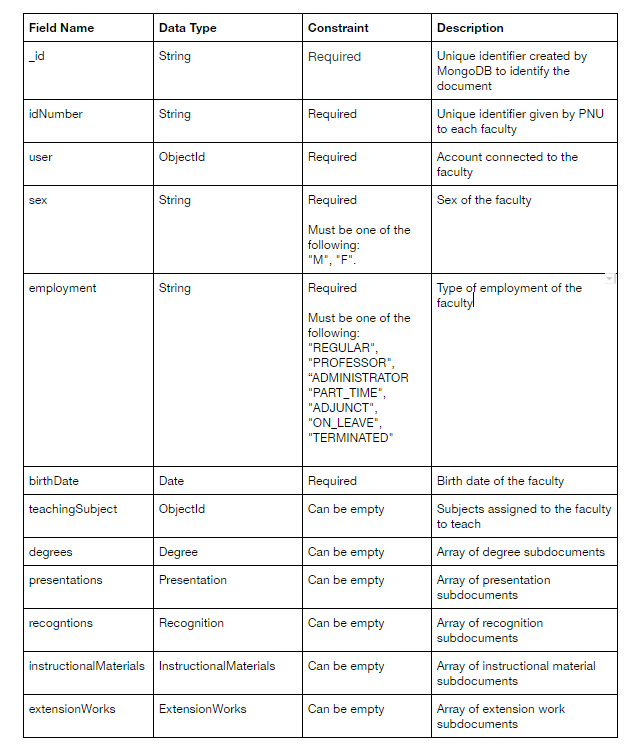
\includegraphics[width=\linewidth]{figures/tables/faculty_table.png}
}

\pagebreak

\subsubsection{Faculty Subdocuments Tables}

Track changes is off
Everyone
skeithtan
Guests
Current file
Overview
1
\makefigure{!ht}{
   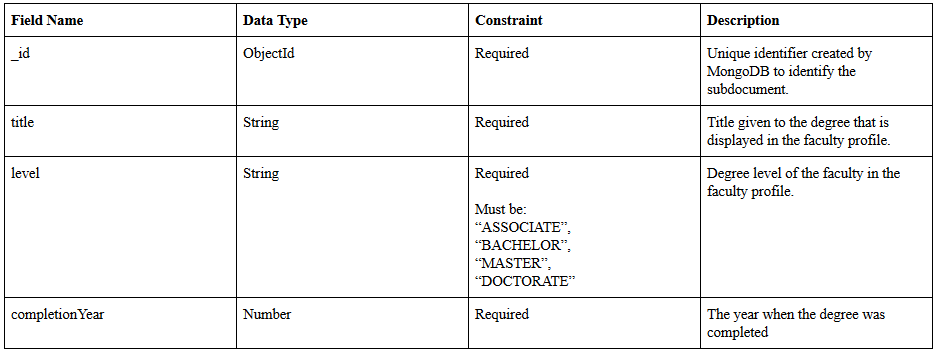
\includegraphics[width=\linewidth]{figures/tables/degree_table.png}
}

\pagebreak

\makefigure{!h}{
   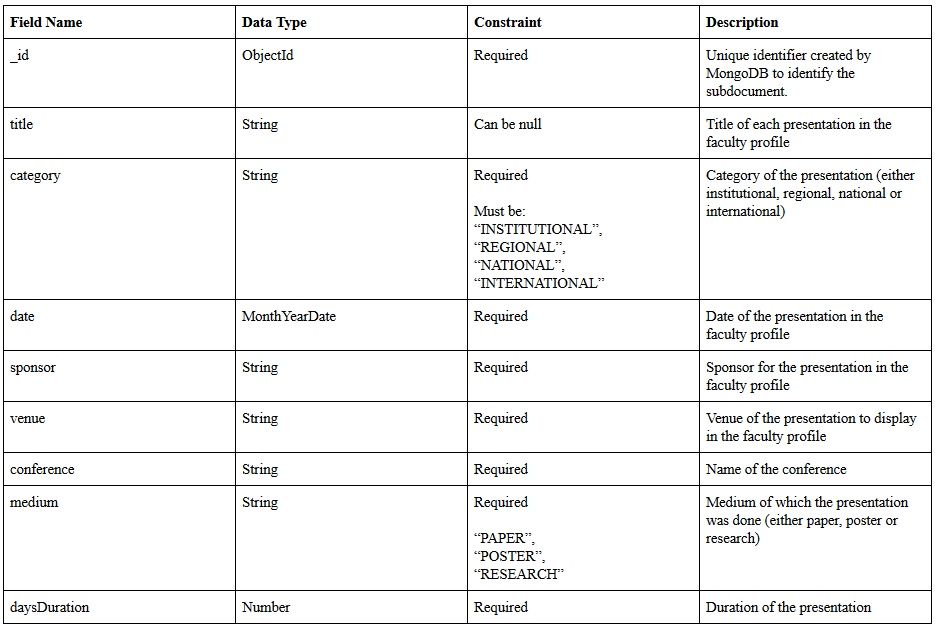
\includegraphics[width=\linewidth]{figures/tables/presentation_table.png}
}

\pagebreak

\makefigure{!h}{
   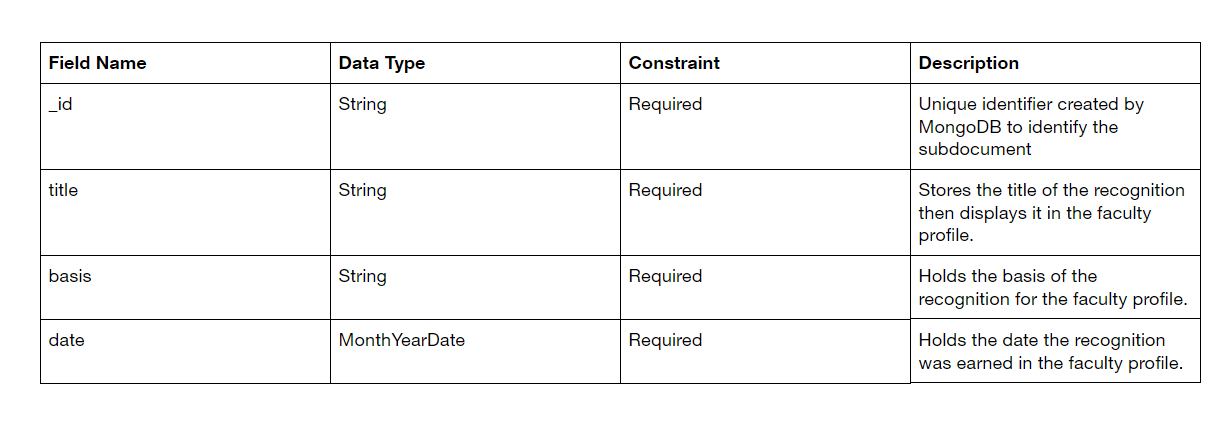
\includegraphics[width=\linewidth]{figures/tables/recognition_table.png}
}

\pagebreak

\makefigure{!h}{
   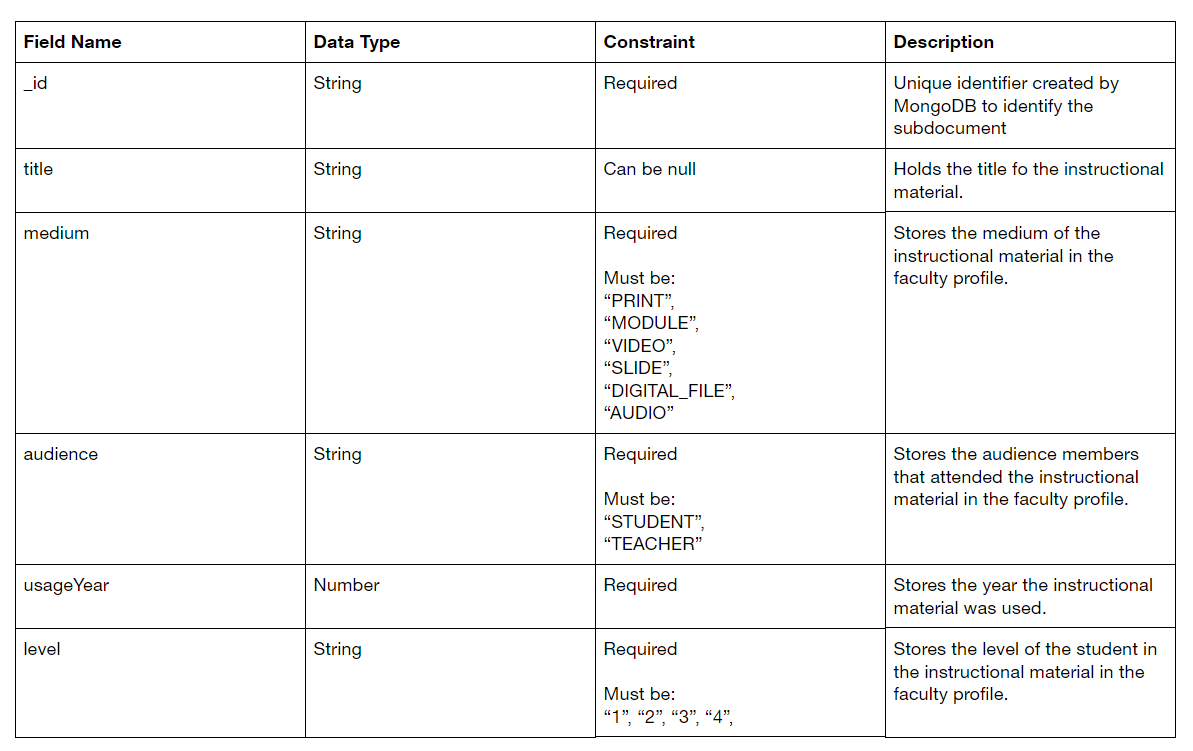
\includegraphics[width=\linewidth]{figures/tables/instructional_table.png}
}

\pagebreak

\makefigure{!h}{
   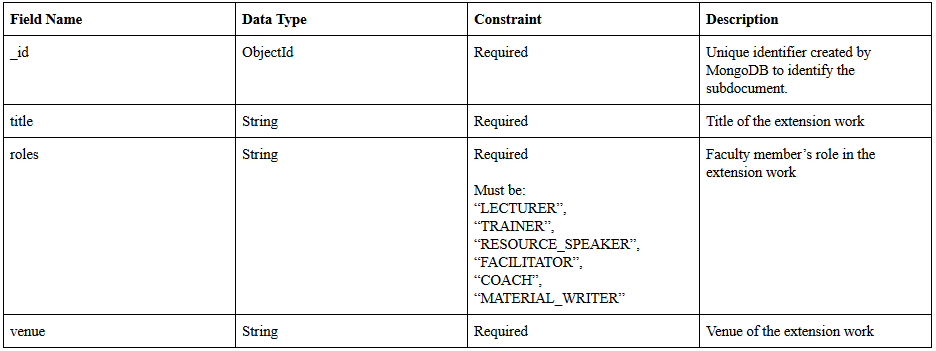
\includegraphics[width=\linewidth]{figures/tables/extension_table.png}
}

\pagebreak


\subsection{Data Coding Standards}

\subsubsection{JavaScript}
\paragraph{Terminating statements}
Semicolons are mandatory whenever terminating a statement in JavaScript. 

\paragraph{Trailing Commas}
In object literals, array literals, function parameters, function call arguments, class extensions, module imports, and the like, trailing commas are mandatory, but only when the literal is written in multiple lines. Single line literals must not have trailing commas.

\paragraph{Module Exports}
Modules must never be exported as default. Even if a file contains only one import, it must still be exported without the default modifier. This ensures name consistency across imports, and allows IDEs to assist in module imports.

\paragraph{Variable Declarations}
Variable declarations must never be declared using the JavaScript keyword \texttt{var}. The default variable declaration should use \texttt{const}, and only changed to \texttt{let} when the variable is expected to change.

\paragraph{Utilities}
Functions and reusable code that do not belong in a particular module, but should be abstracted are classified as a utility. These utilities are given their own folder in both the server and the client and must be stored in these folders.

\paragraph{File and Folder Naming}
Files and Folders must be in snake case. 

\paragraph{Classes Naming}
Classes must be in pascal case.

\paragraph{Functions and Variable Naming}
Functions and variables must be in camel case.

\paragraph{Spaces}
Indentations must be done with 4 spaces and not tabs.

\paragraph{Arrow Functions}
Arrow functions are used to make the code shorter and more readable.

\subsubsection{Client}

\paragraph{Exporting React Components}
React components must be enclosed in their own folder. The snake case convention is overridden in this scenario; the folder and the file that contain the React component must use the same name as the React component itself. The folder must include an \texttt{index.js} file which exposes the React Component. Any other file importing this component must import the component through the \texttt{index.js} file. This is because the \texttt{index.js} file may include styling, connection to redux, or a connection to React router.

\paragraph{React Components}
React components must be written as a pure component if possible. If the component uses lifecycle functions such as \texttt{componentWillMount()}, the component may use ES6 class syntax, inheriting from \texttt{PureComponent}. If the component is stateless and only has a render function, the component should be written in function pure component form.

\paragraph{React Component Classes Instance Functions and Properties}
Instance functions in React component classes, with the exception of lifecycle methods such as \texttt{componentWillMount()} must be written in the shorthand function syntax. Instance properties such as the default state must be written as a direct assignment.

\paragraph{URL Paths}
URL paths must be written in kebab case. 

\subsubsection{Server}
\paragraph{GraphQL Type Definitions}
GraphQL type definitions must be defined in its own separate \texttt{.graphql} files and not as JavaScript string literals. This allows text editors to perform syntax highlighting on the GraphQL code.


\section{Screen Specifications}
    \subsection{Sign In}
    \field{Screen Name} {Sign In}
    
    \field{File Name}{/pages/SignIn/index.js}
    
    \field{Description}{Where users must enter their Email address and password to access the system.}
    
    \field{Layout}{}
    
    
\makefigure{!h}{
   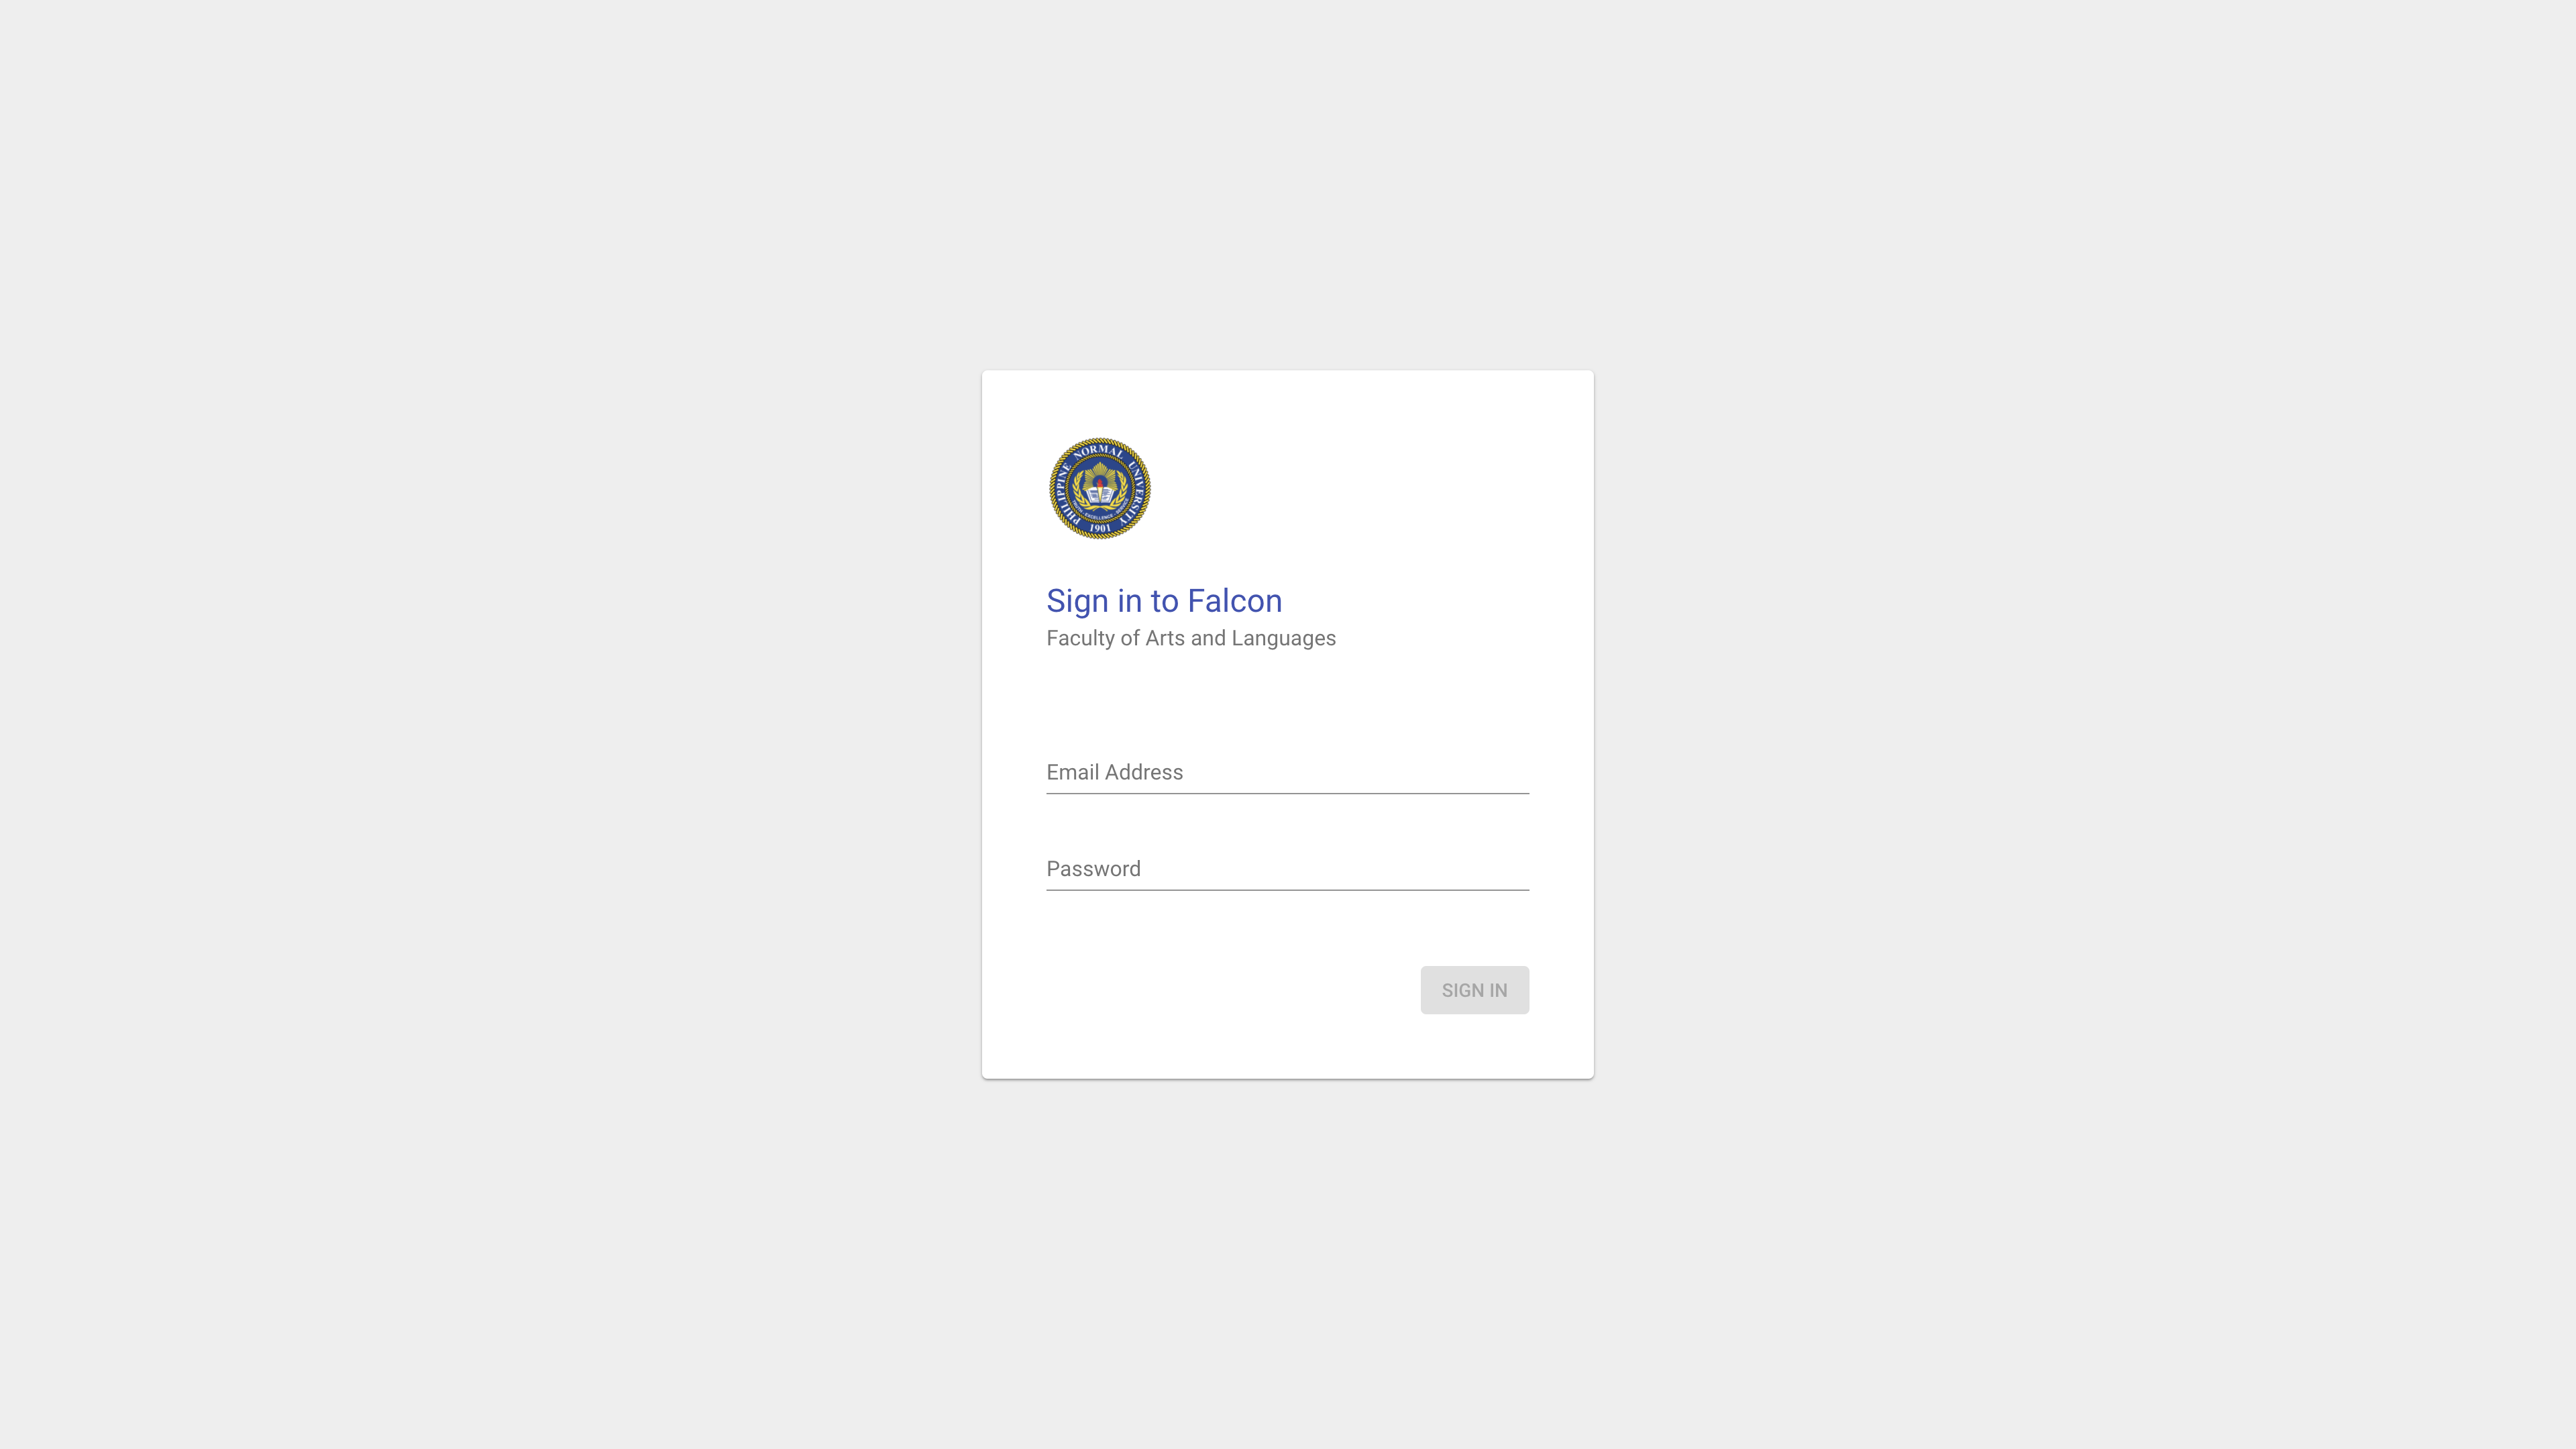
\includegraphics[width=\linewidth]{figures/screen_specifications/sign_in.png}
   \caption{Sign In Screen}
}
    \pagebreak

    \subsection{Faculty Profile}
    
    \subsubsection{Faculty Overview}
    \field{Screen Name} {Faculty Overview}
    
    \field{File Name}{/pages/FacultyProfiles/index.js}
    
    \field{Description}{Displays the details of the faculty member. First card contains the basic information, second card contains the subject assignments, third card contains the degrees, and fourth card contains the recognitions.}
    
    \field{Layout}{}
    
    
\makefigure{!h}{
   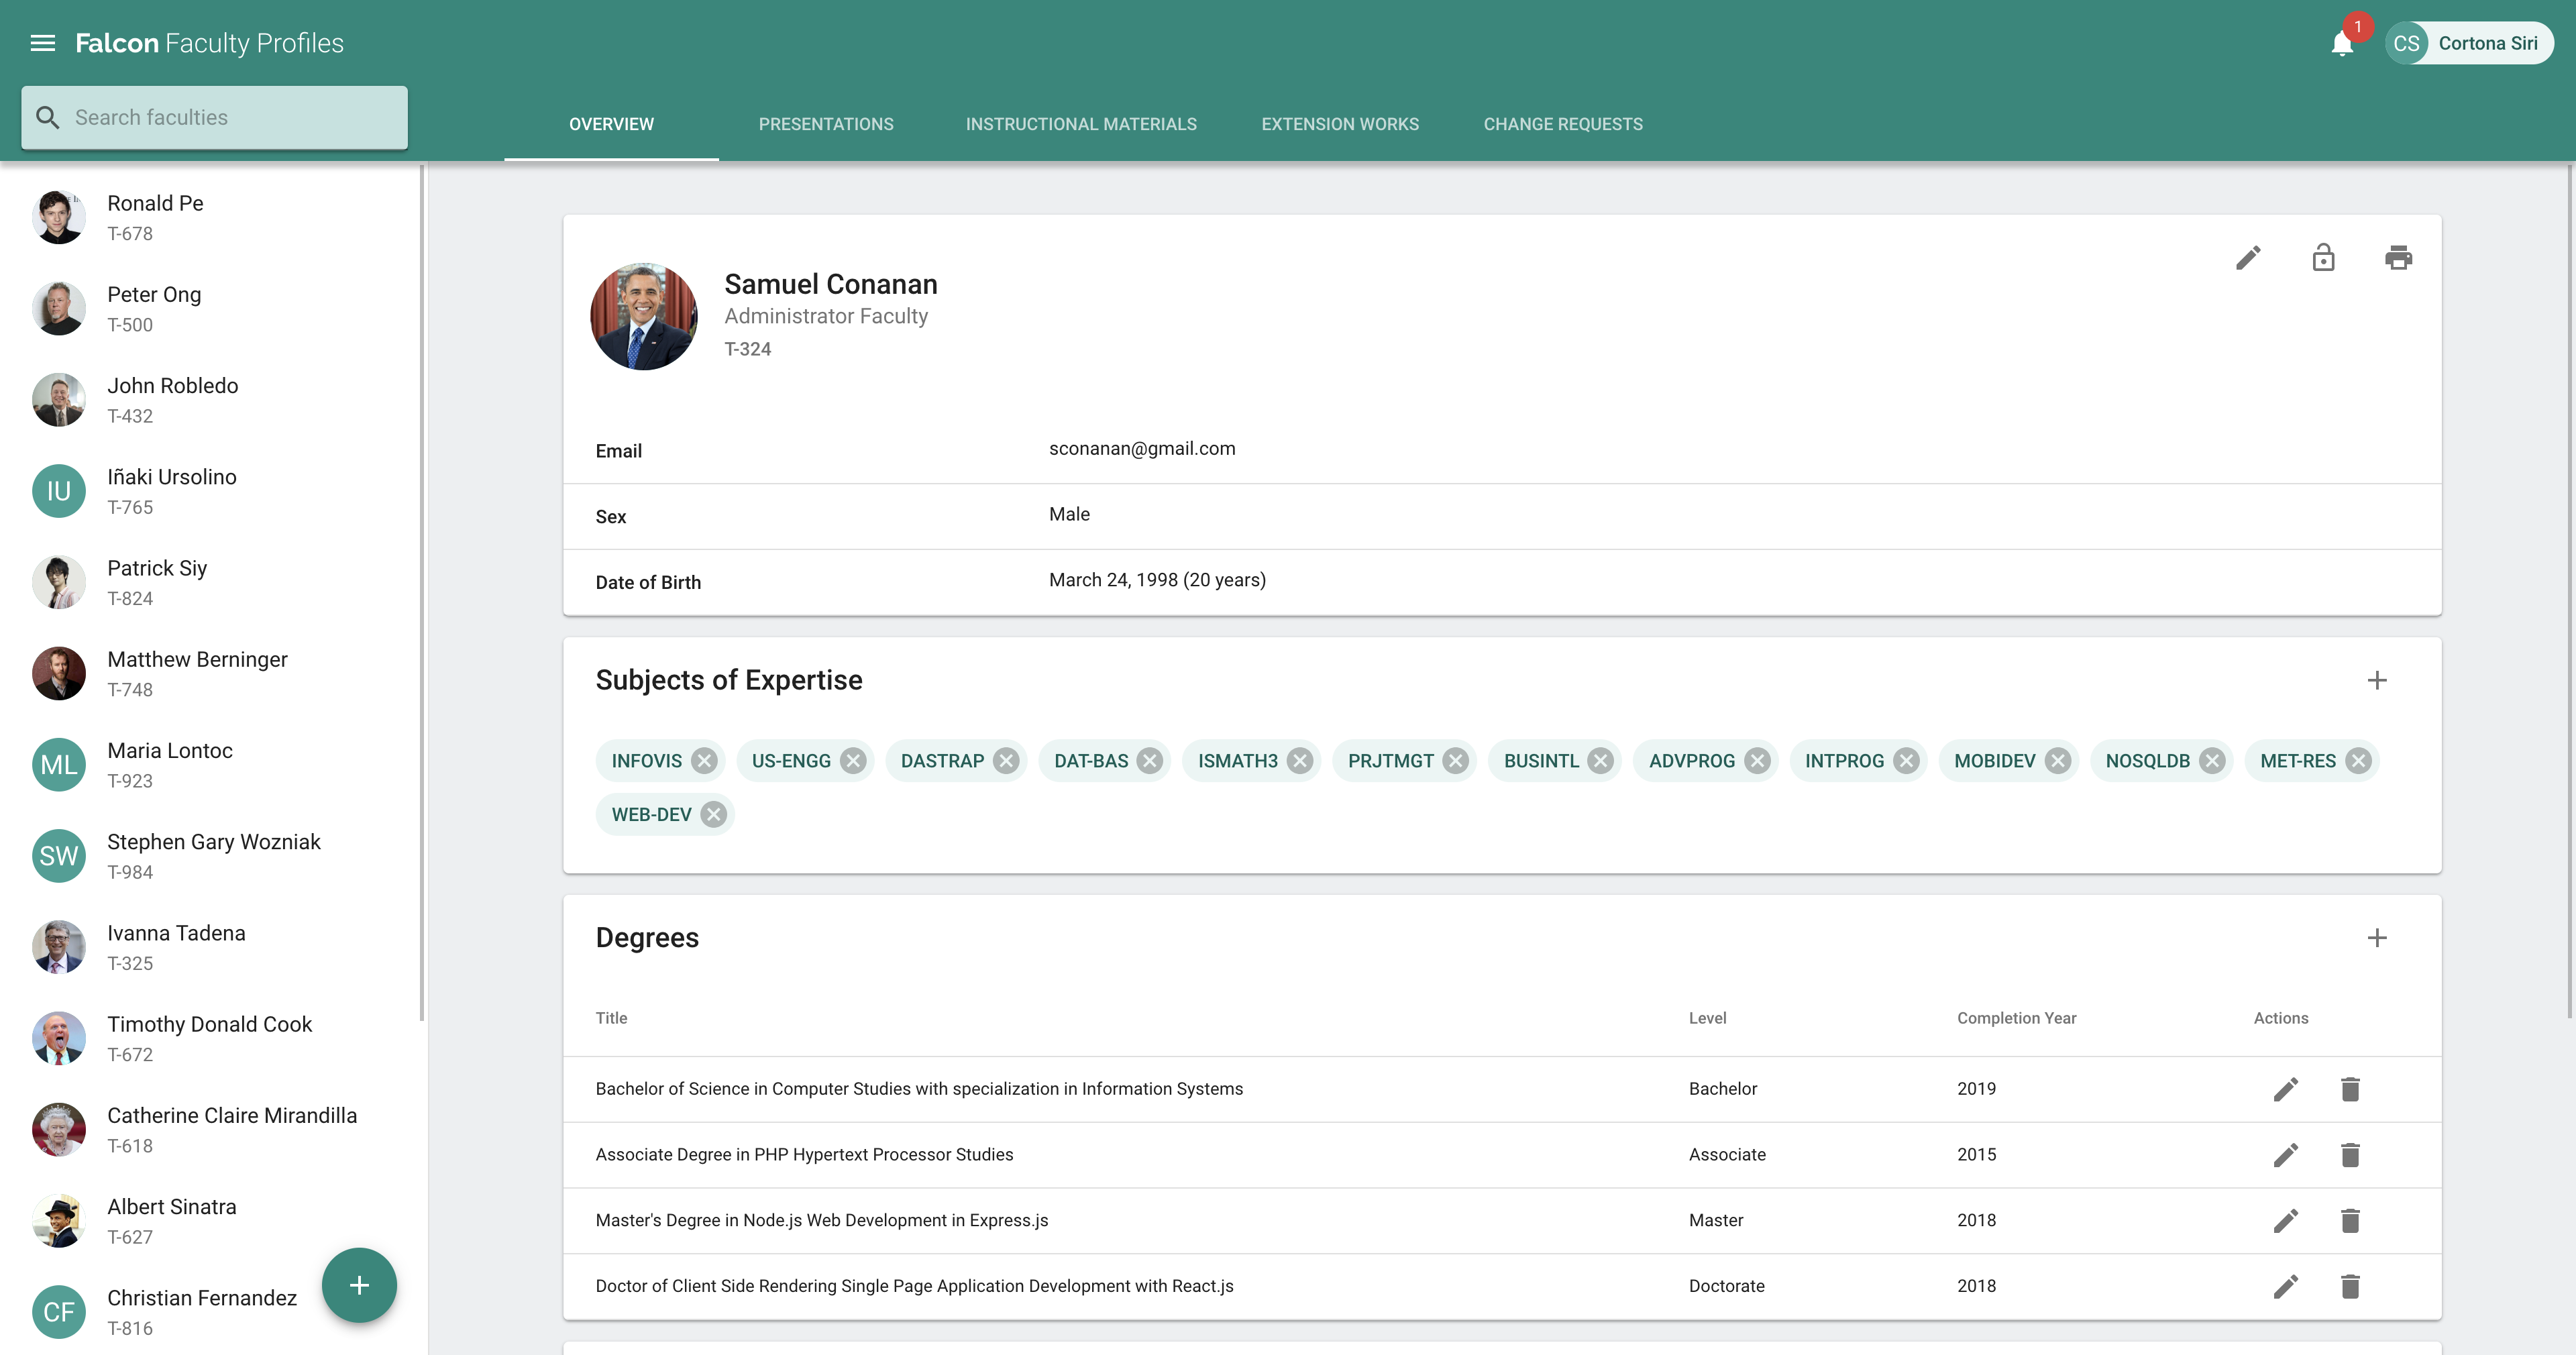
\includegraphics[width=\linewidth]{figures/screen_specifications/faculty_profile1.png}
   \caption{Faculty Profile Screen A}
}

\pagebreak

\makefigure{!h}{
   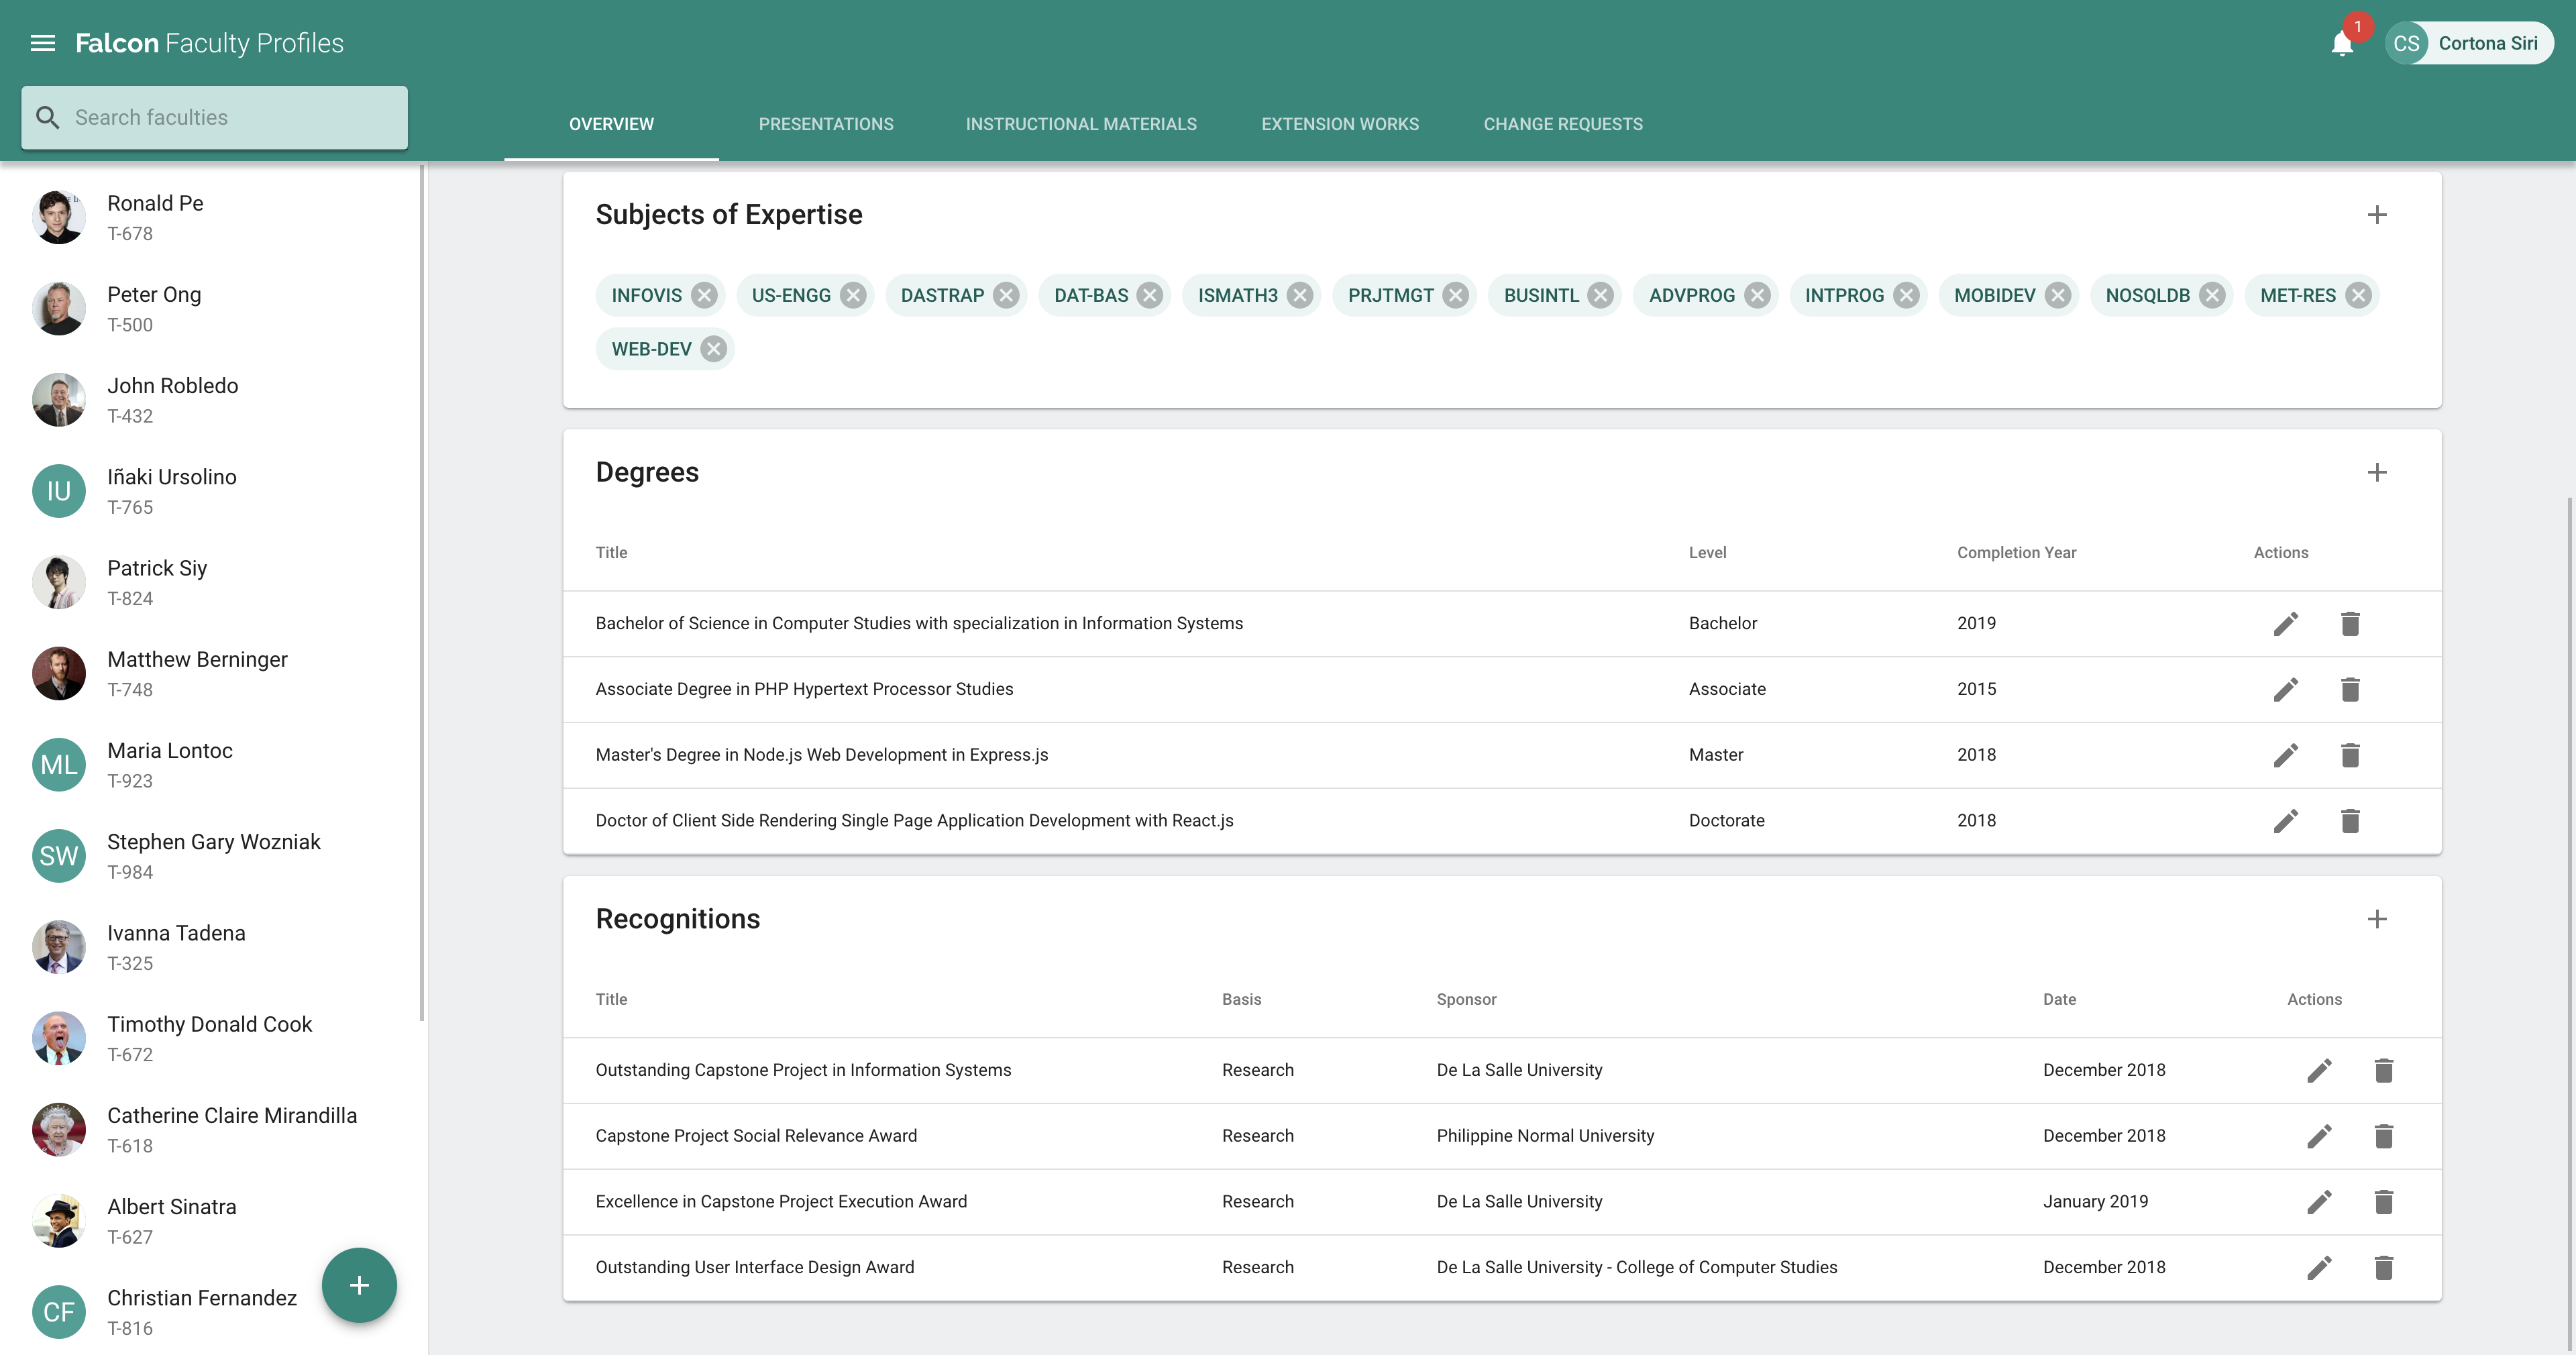
\includegraphics[width=\linewidth]{figures/screen_specifications/faculty_profile2.png}
   \caption{Faculty Profile Screen B}
}

\pagebreak

\subsubsection{Remove Degree}
    
    \field{Screen Name}{Remove Degree}
    
    \field{File Name}{/pages/FacultyProfiles/components/modals/RemoveDegreeModal/index.js}
    
    \field{Description} {Warns the clerk or dean to confirm if they want to remove the degree from the faculty profile.}
    
    \field{Layout}{}
    
\makefigure{!h}{
   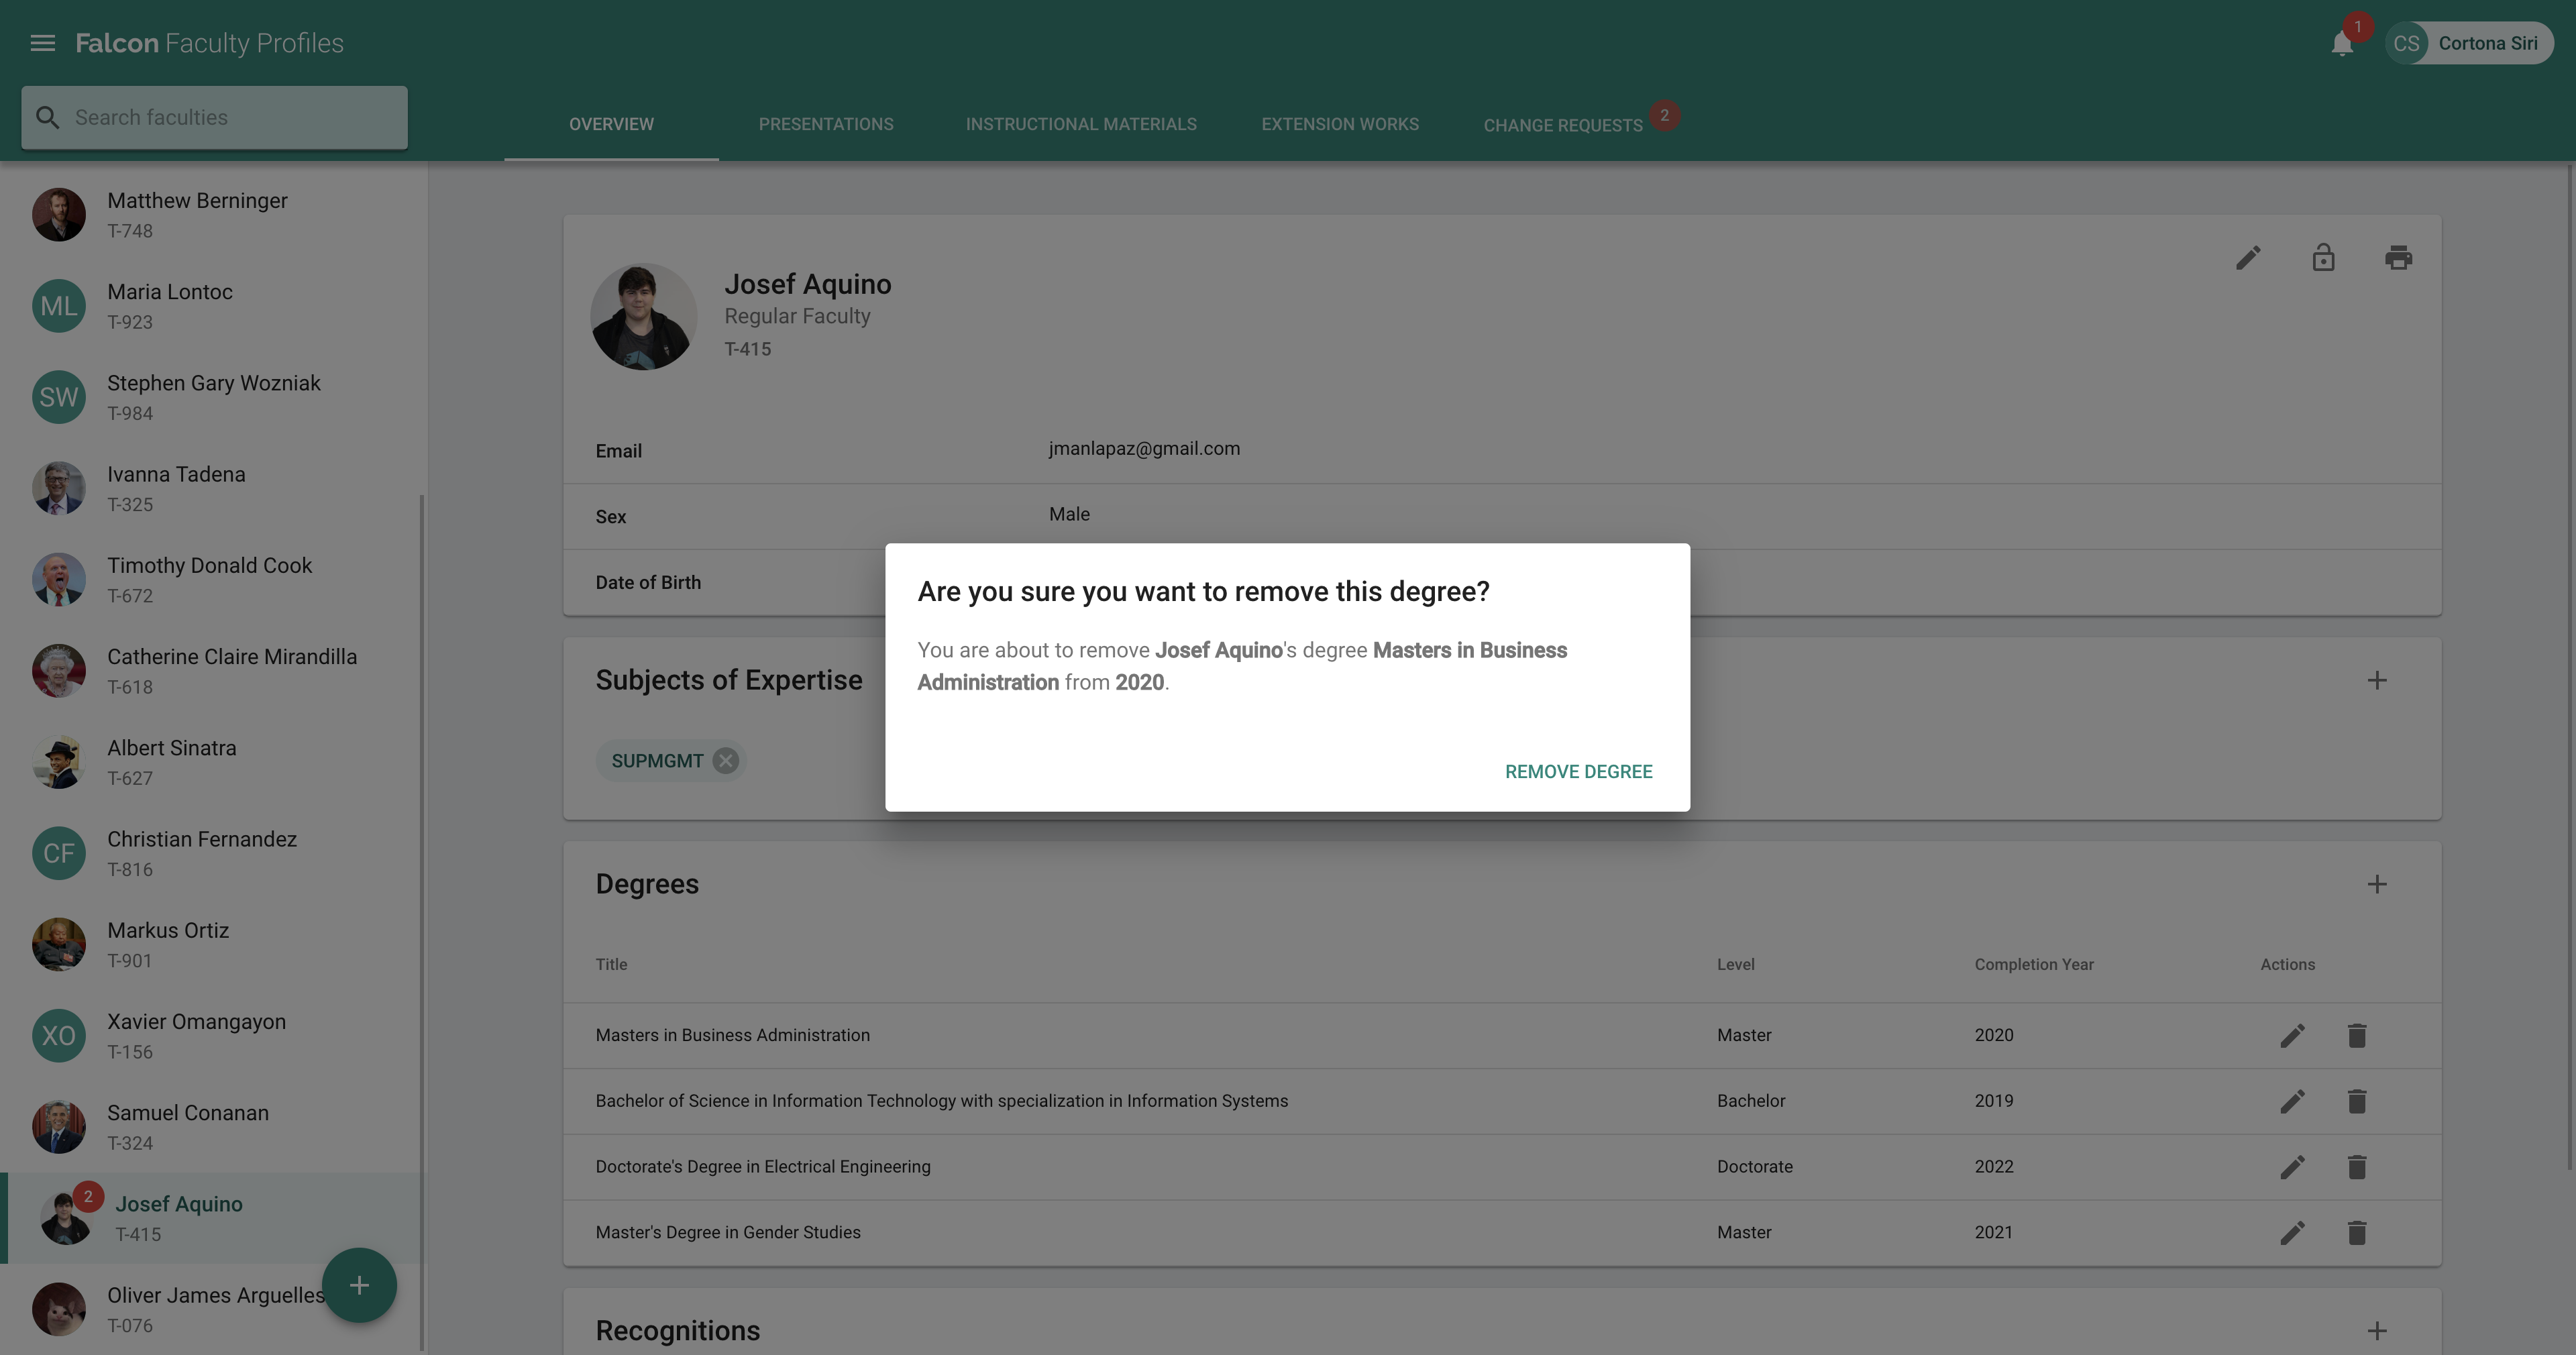
\includegraphics[width=\linewidth]{figures/screen_specifications/remove_degree.png}
   \caption{Remove Degree Screen}
   }
   
   \pagebreak
   
    \subsubsection{Remove Recognitions}
    
    \field{Screen Name}{Remove Recognitions}
    
    \field{File Name}{/pages/FacultyProfiles/components/modals/RemoveRecognitionModal/index.js}
    
    \field{Description} {Confirm if the clerk or dean wants to remove the recognition from the faculty profile.}
    
    \field{Layout}{}
    
\makefigure{!h}{
   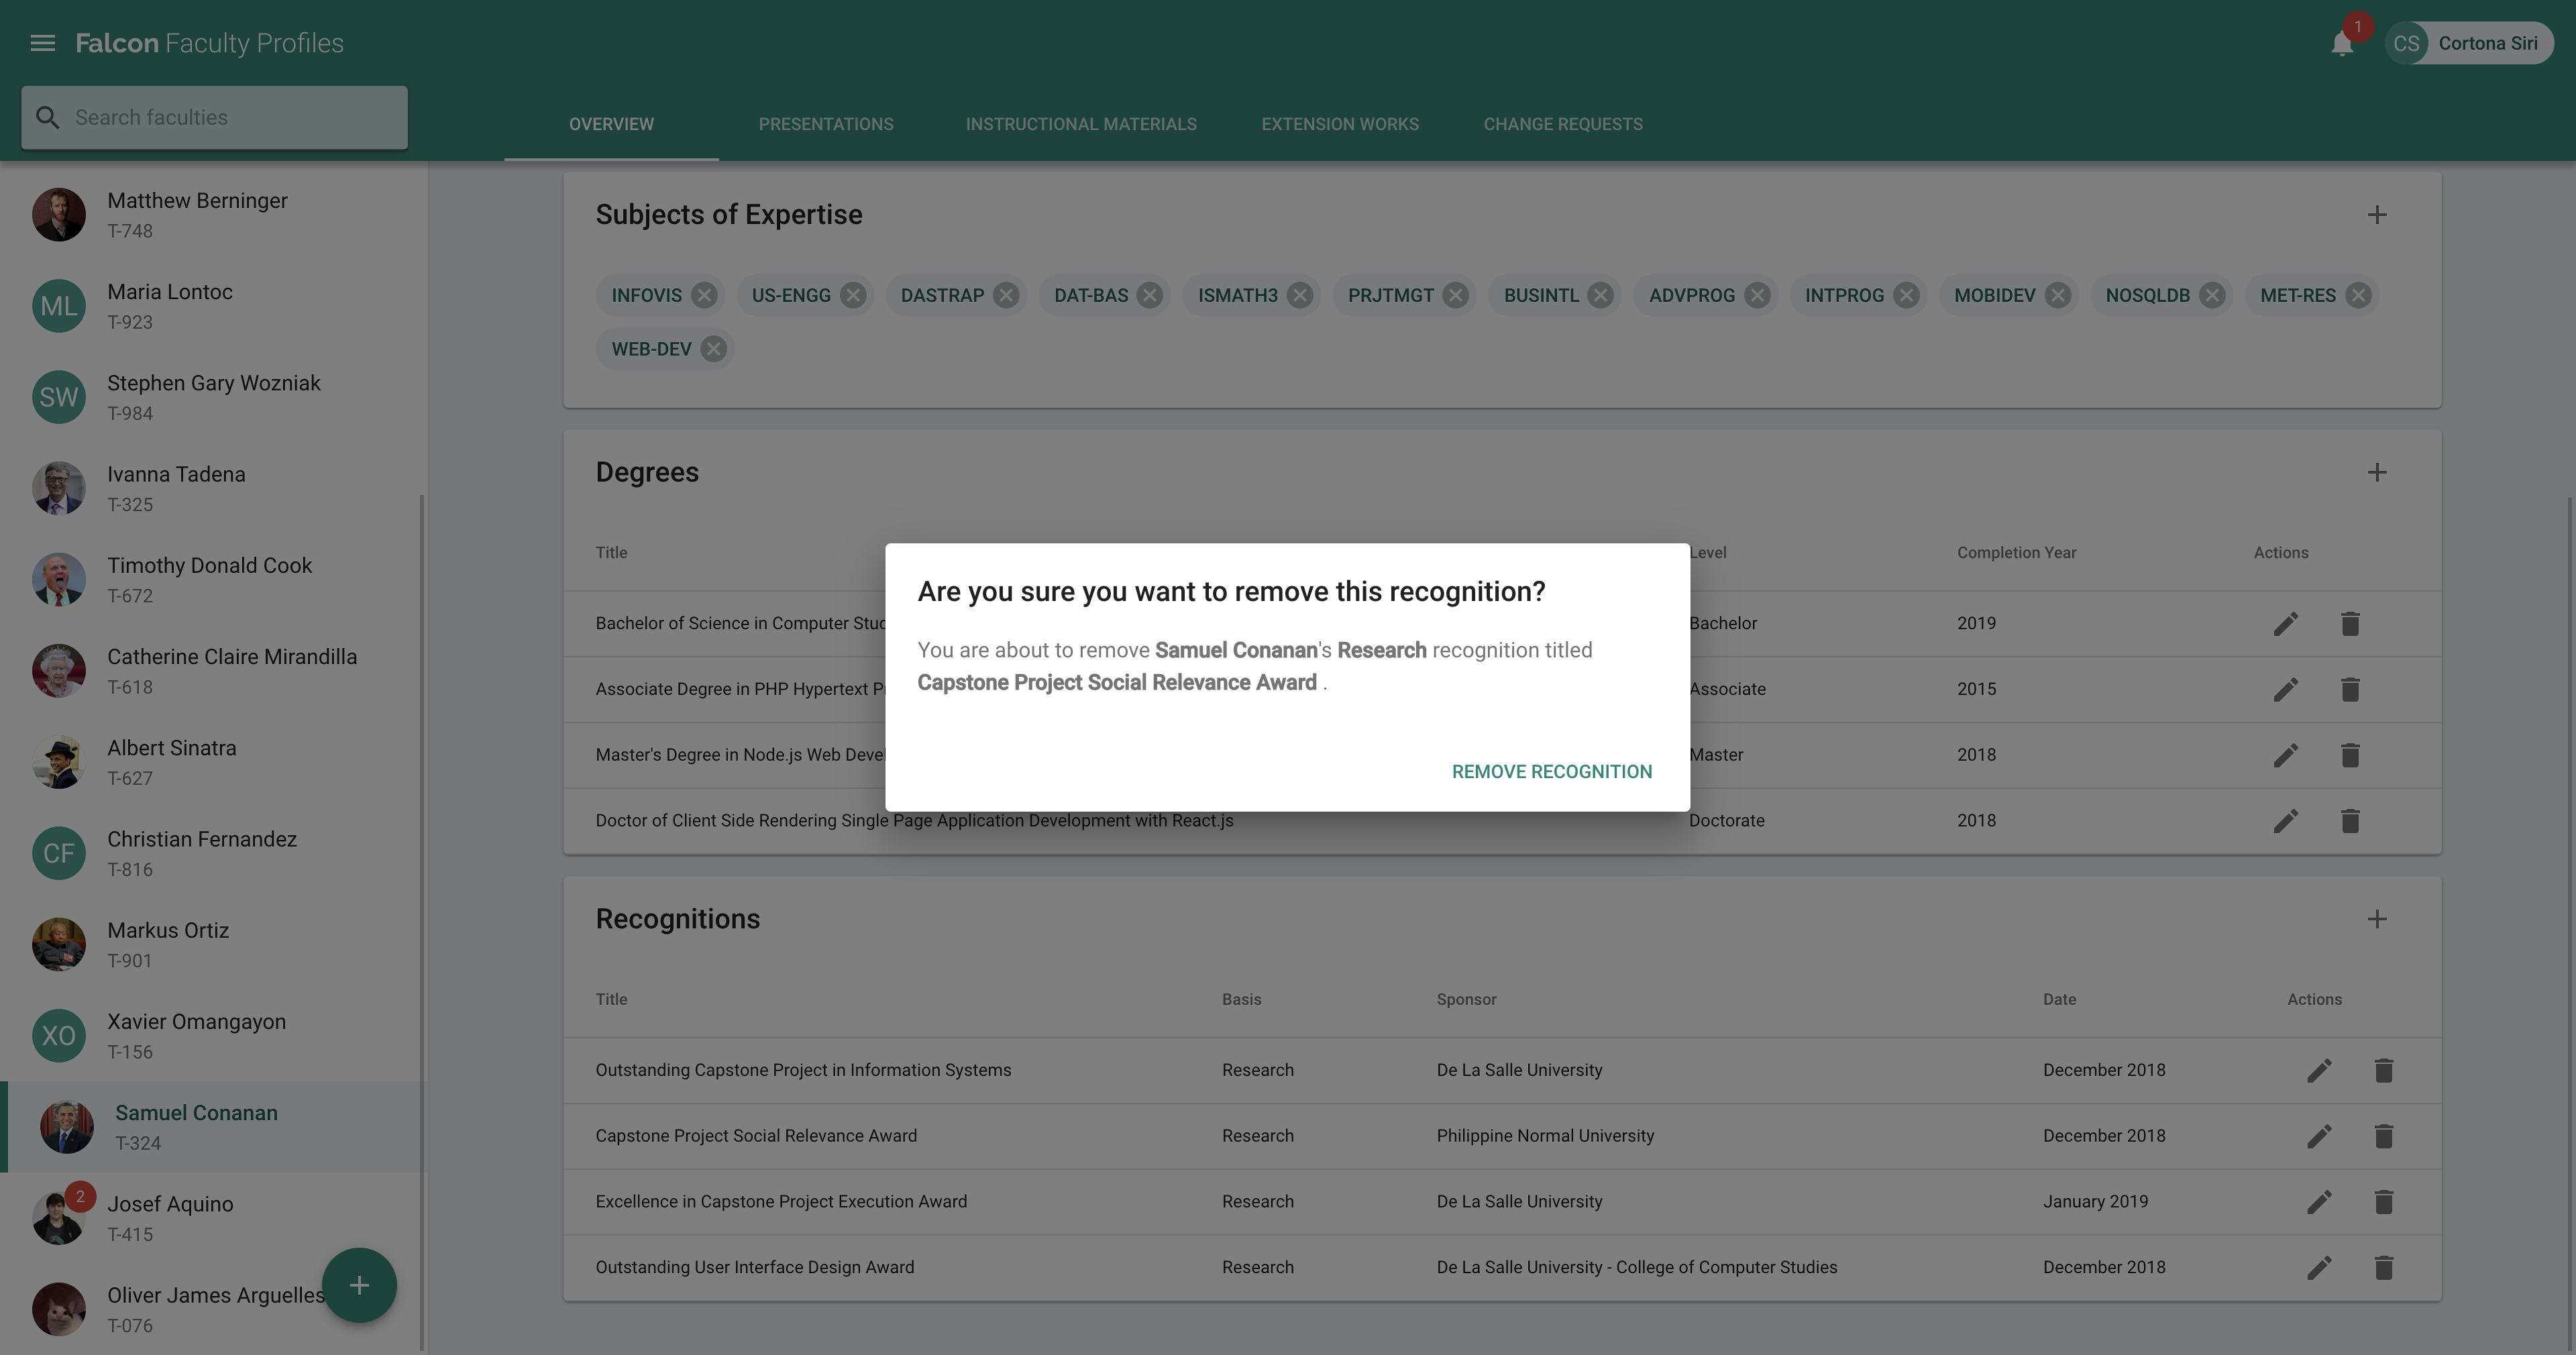
\includegraphics[width=\linewidth]{figures/screen_specifications/components/modals/remove_recognition.png}
   \caption{Remove Recognition Screen}
   }
   
   \pagebreak
   
    \subsubsection{Print Preview}
    
    \field{Screen Name}{Print Preview}
    
    \field{File Name}{/pages/FacultyProfiles/ProfilePrintPreview/index.js}
    
    \field{Description} {Shows the clerk or dean a preview of the report. Also allows the user to select which kind of information to include in the report.}
    
    \field{Layout}{}
    
\makefigure{!h}{
   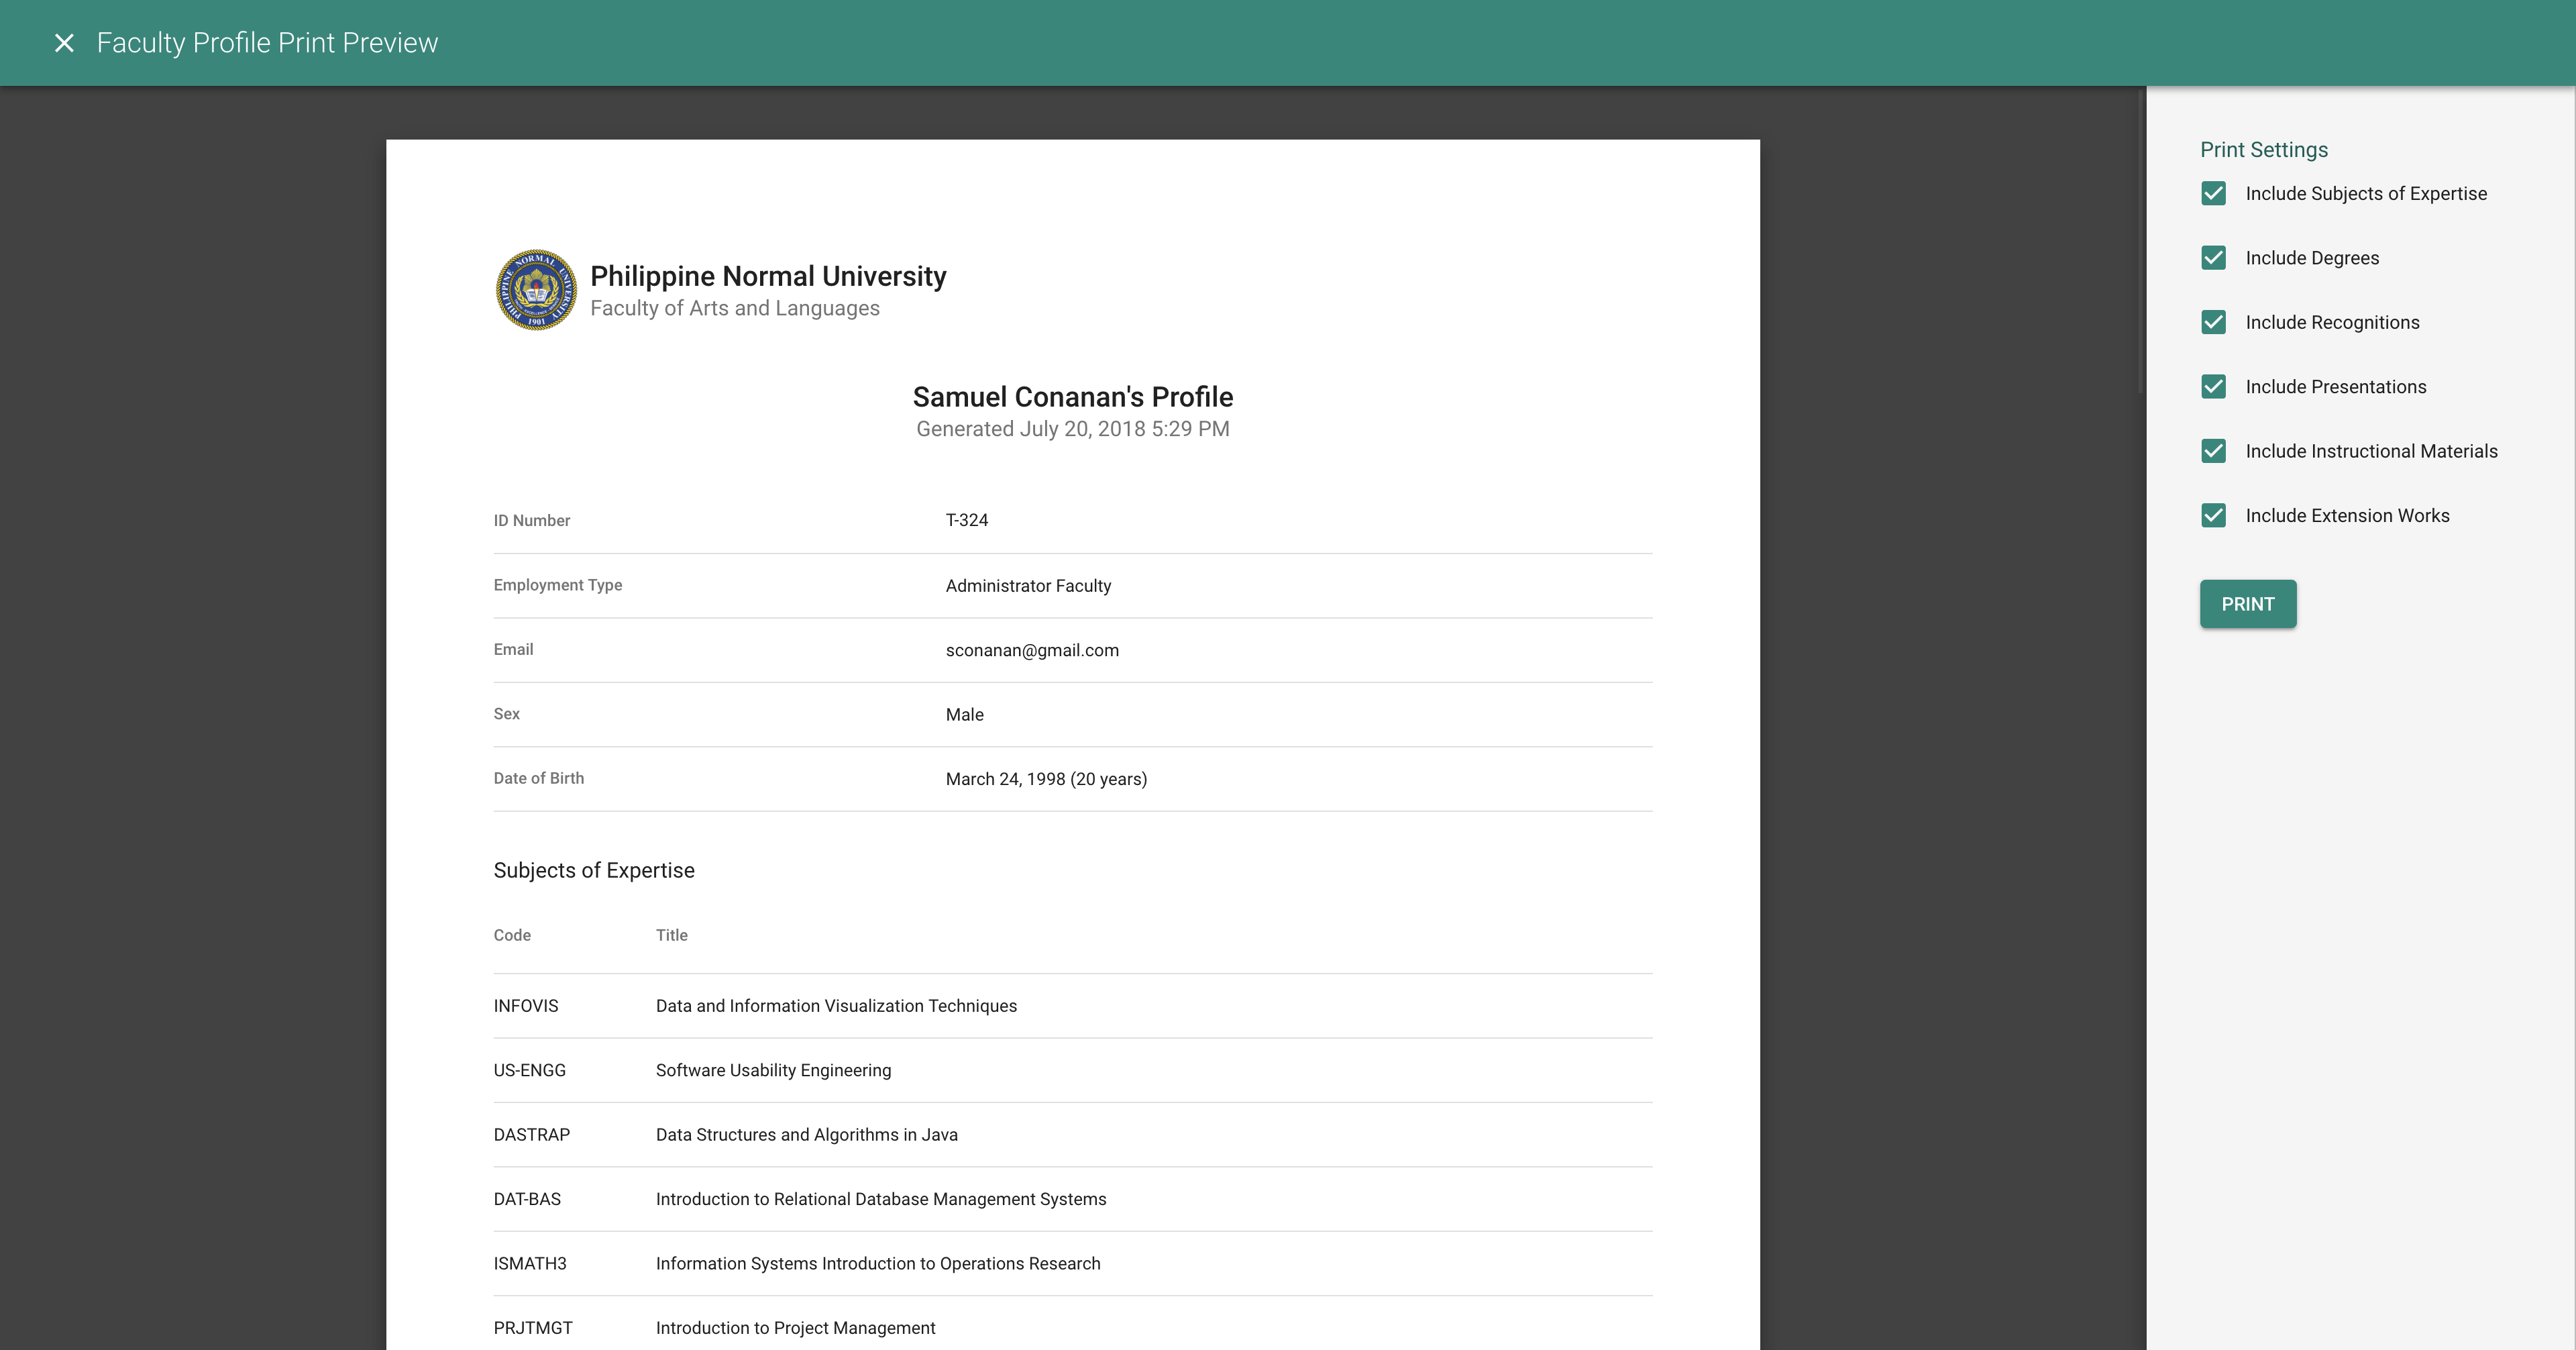
\includegraphics[width=\linewidth]{figures/screen_specifications/print_preview.png}
   \caption{Print Preview Screen}
   }
   
   \pagebreak
   
   \subsubsection{Reset Password}
    
    \field{Screen Name}{Reset Password}
    
    \field{File Name}{/pages/FacultyProfiles/components/modals/ResetPasswordModal/index.js}
    
    \field{Description} {Allows the clerk or dean to reset the password of a faculty member through the faculty profile.}
    
    \field{Layout}{}
    
\makefigure{!h}{
   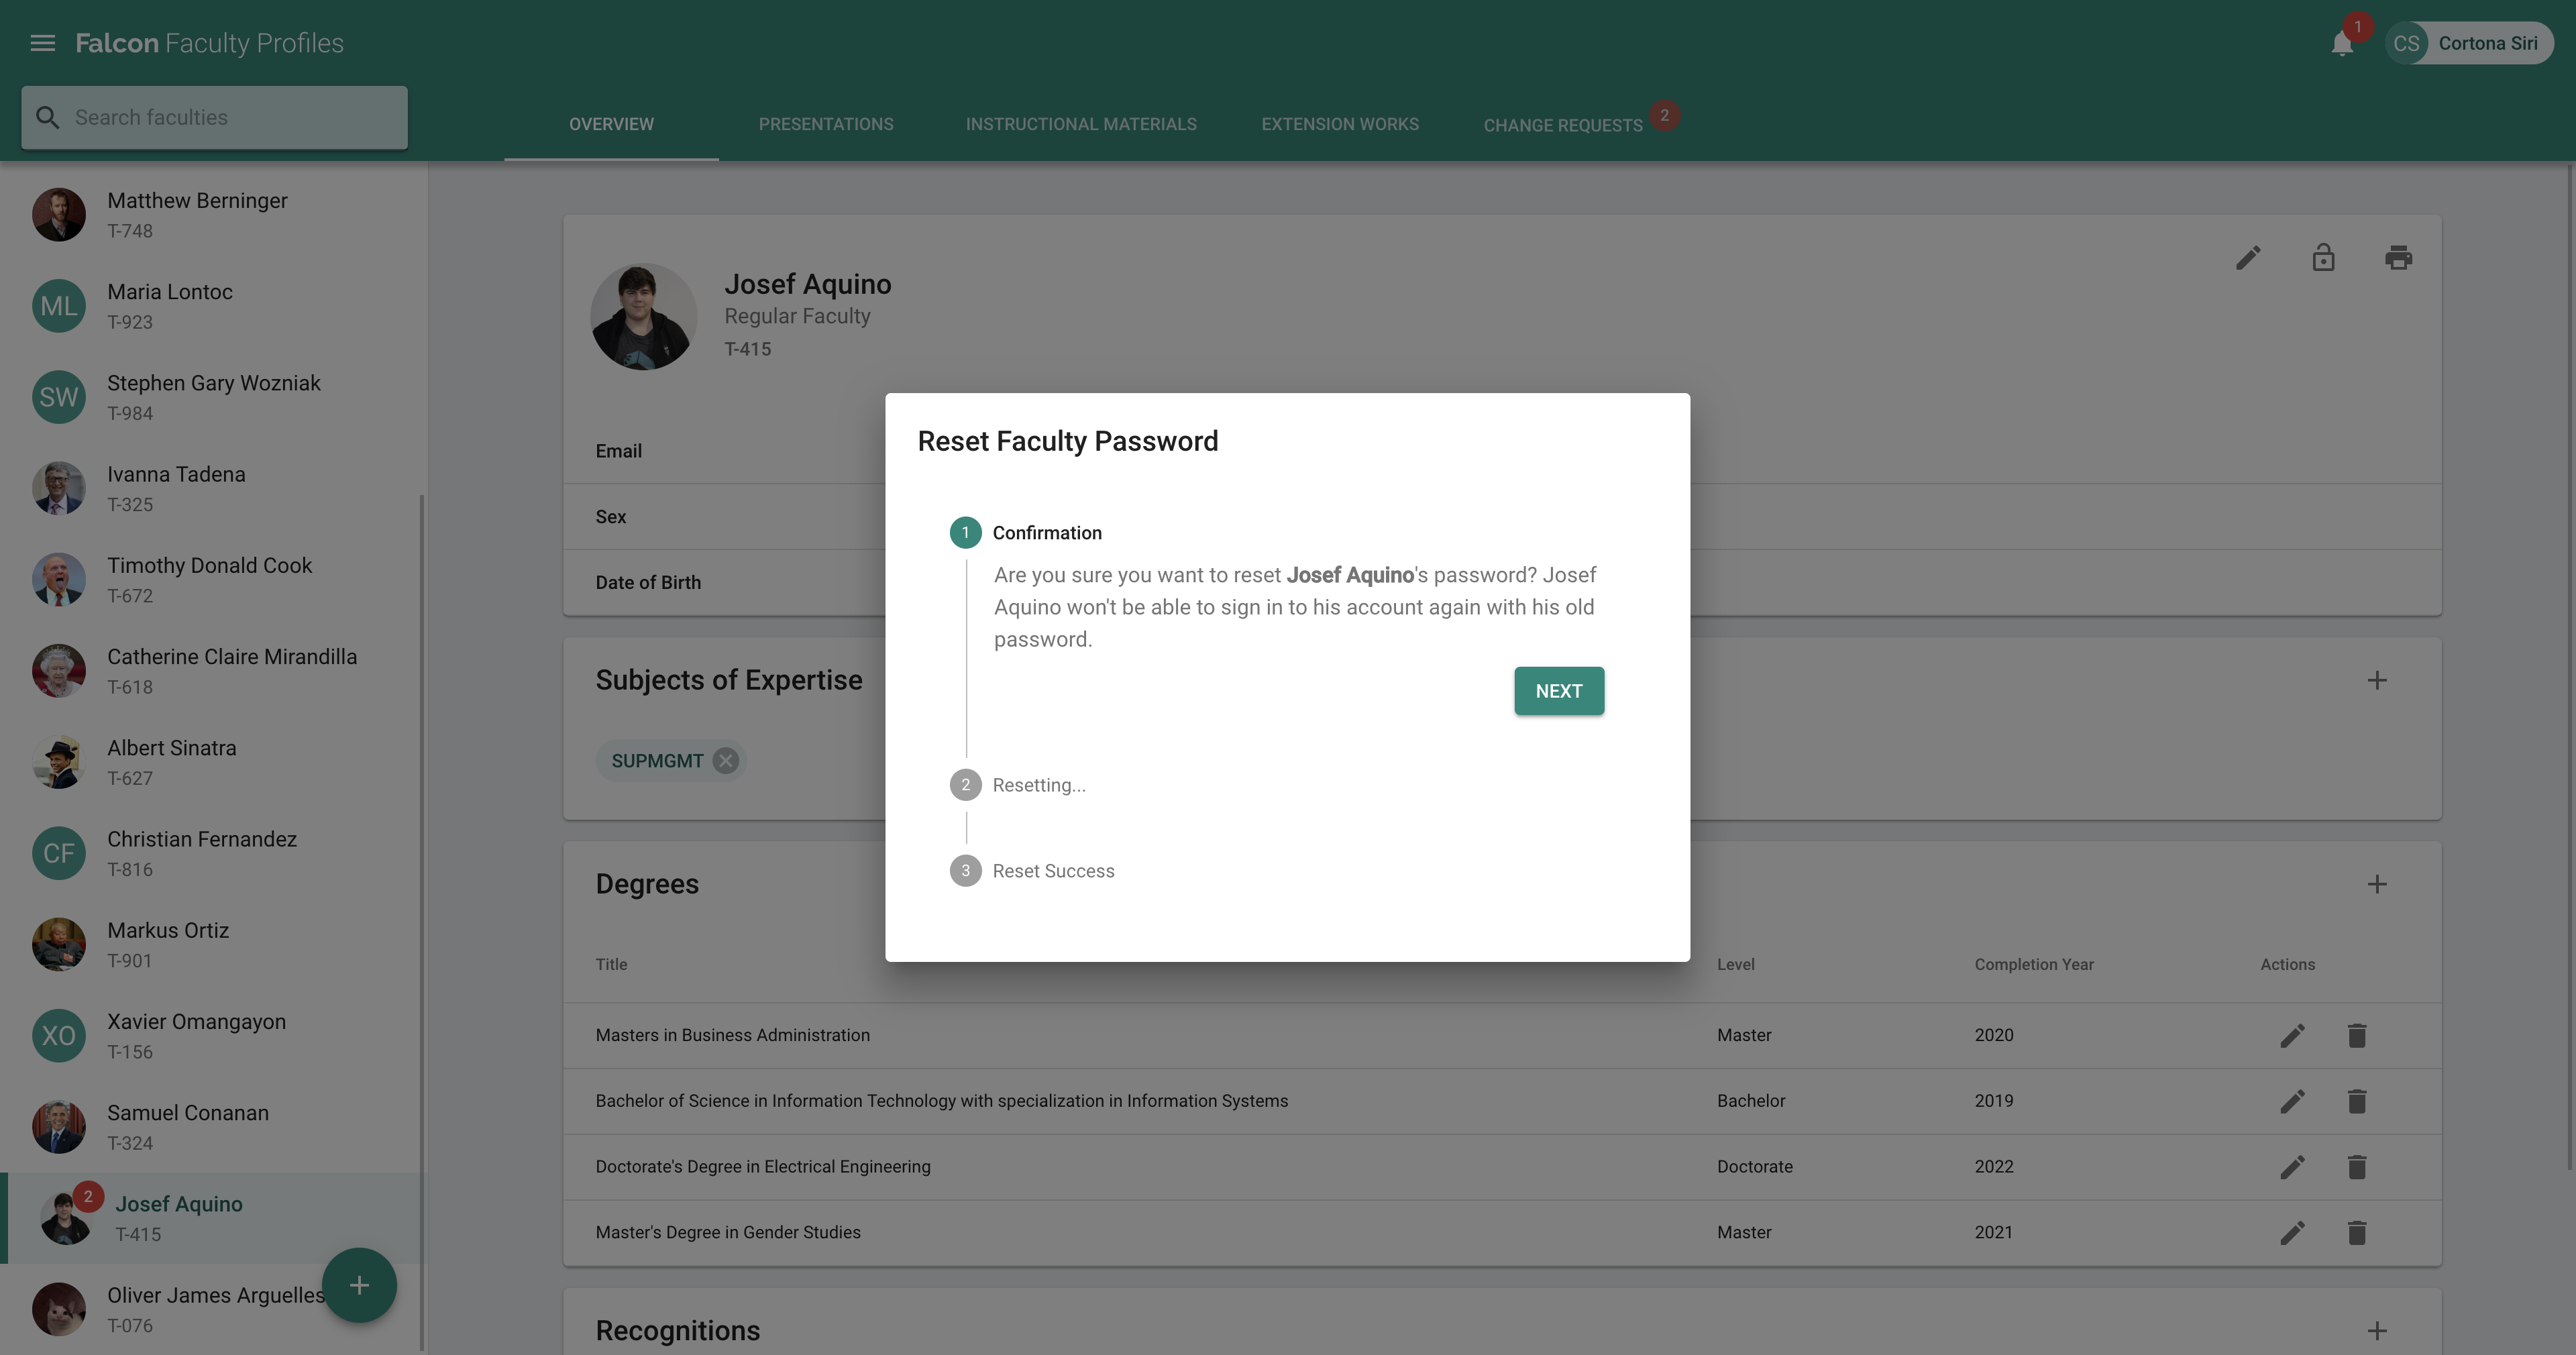
\includegraphics[width=\linewidth]{figures/screen_specifications/reset_password1.png}
   \caption{Reset Password Screen A}
   }
   \pagebreak
   
   \makefigure{!h}{
   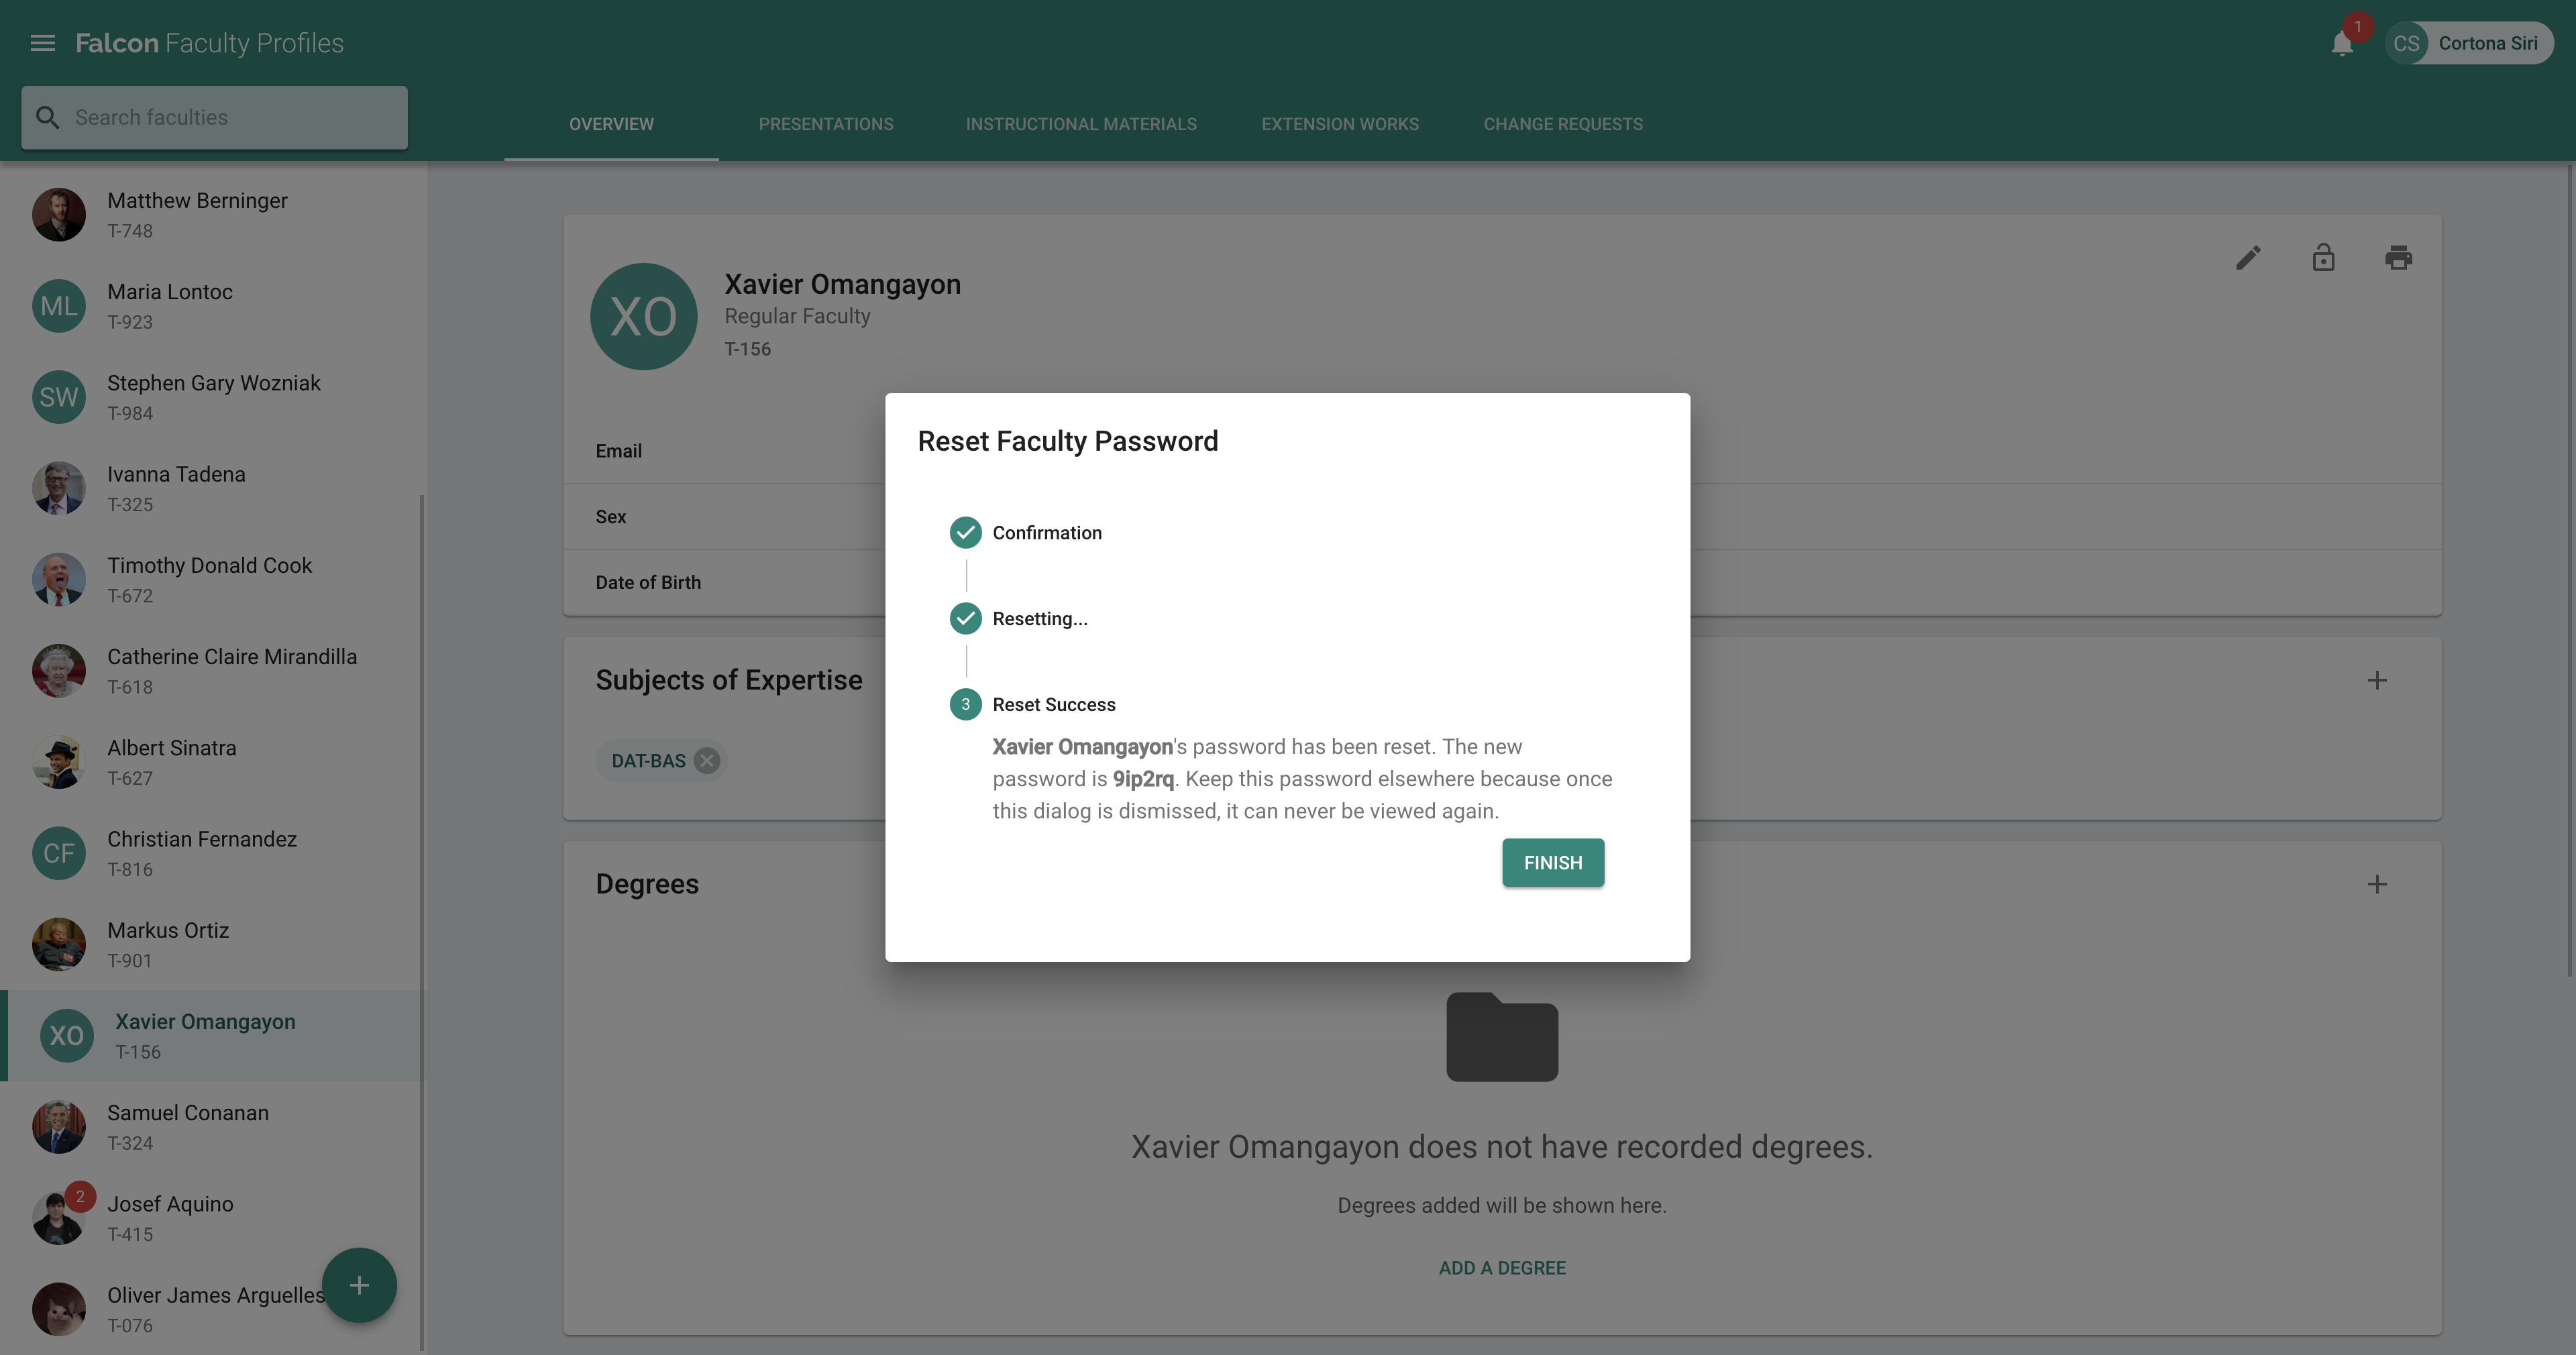
\includegraphics[width=\linewidth]{figures/screen_specifications/reset_password2.png}
   \caption{Reset Password Screen B}
   }
   
   \pagebreak
    
    \subsubsection{Presentations}
    
    \field{Screen Name}{Presentations}
    
    \field{File Name}{/pages/FacultyProfiles/components/faculty_detail_tabs/PresentationsTab/index.js}
    
    \field{Description} {Displays the list of presentations of the faculty profile with the details of each presentation, such as the category, date, sponsor, venue, conference, medium, and duration.}
    
    \field{Layout}{}
    
\makefigure{!h}{
   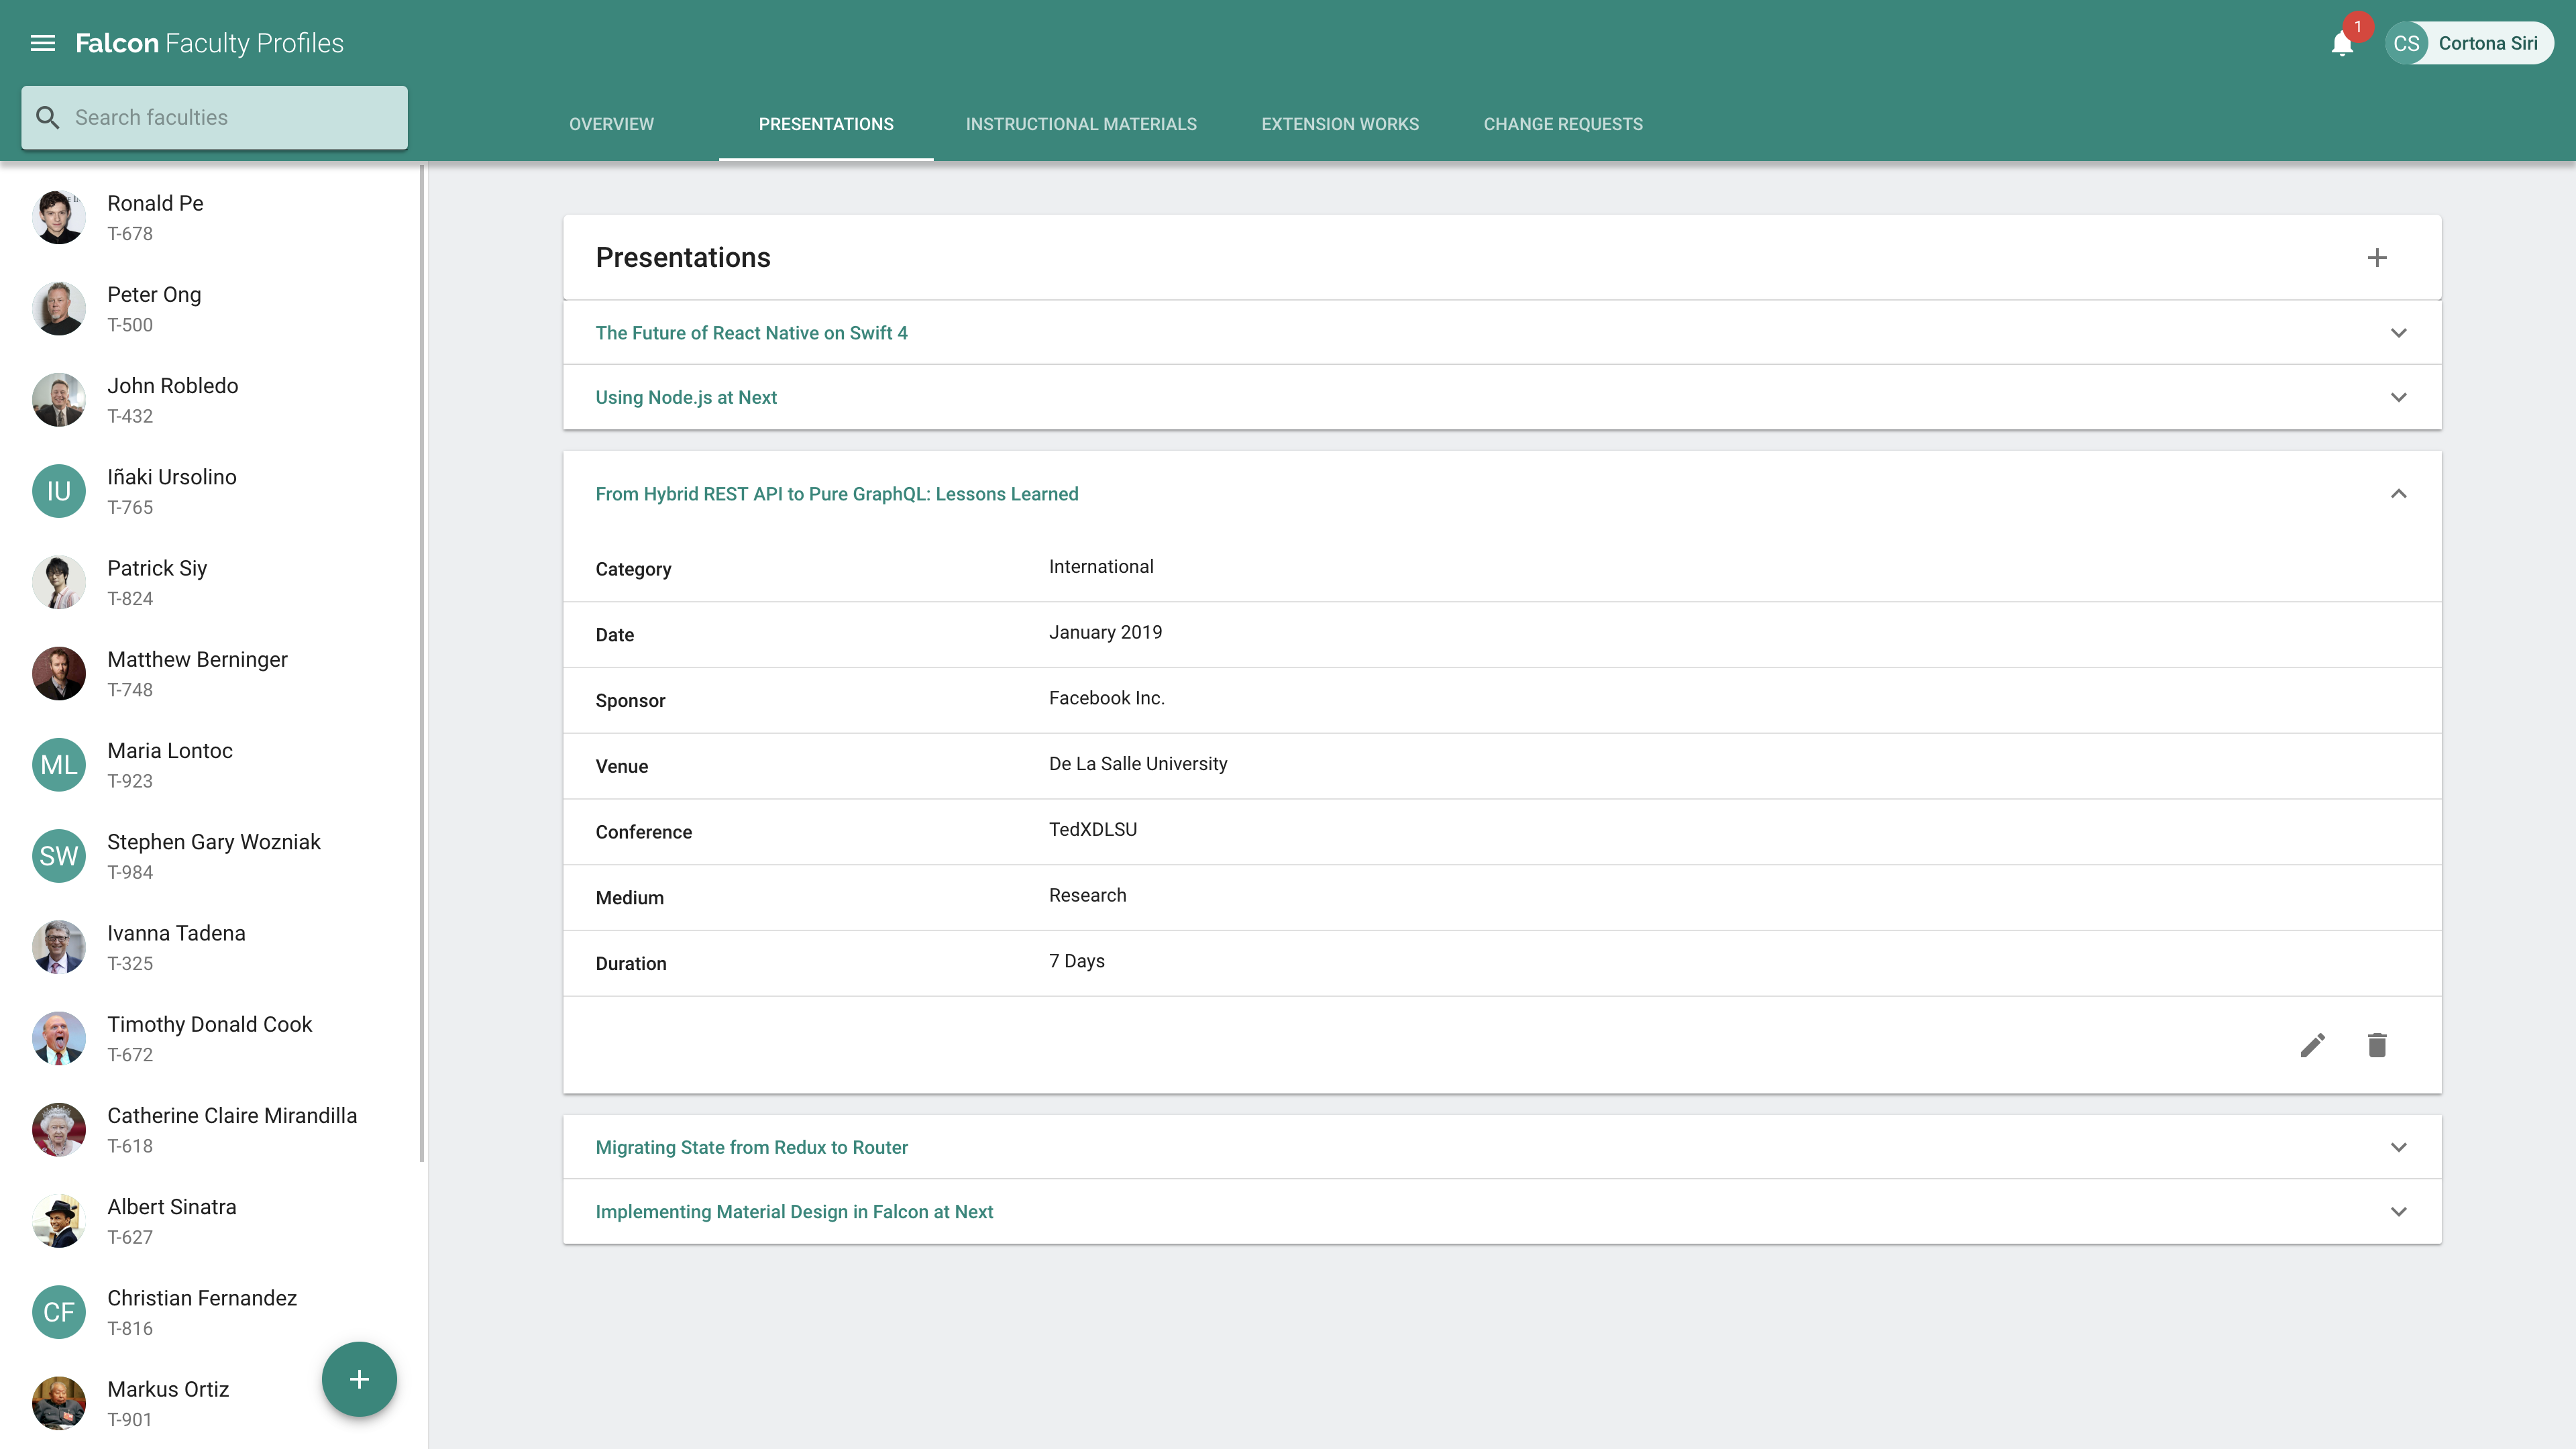
\includegraphics[width=\linewidth]{figures/screen_specifications/presentations.png}
   \caption{Presentations Screen}
   }
   
   \pagebreak
   
   \subsubsection{Remove Presentations}
    
    \field{Screen Name}{Remove Presentations}
    
    \field{File Name}{/pages/FacultyProfiles/components/modals/RemovePresentationModal/index.js}
    
    \field{Description} {To confirm the removal of the presentations on the faculty profile by the clerk or dean.}
    
    \field{Layout}{}
    
\makefigure{!h}{
   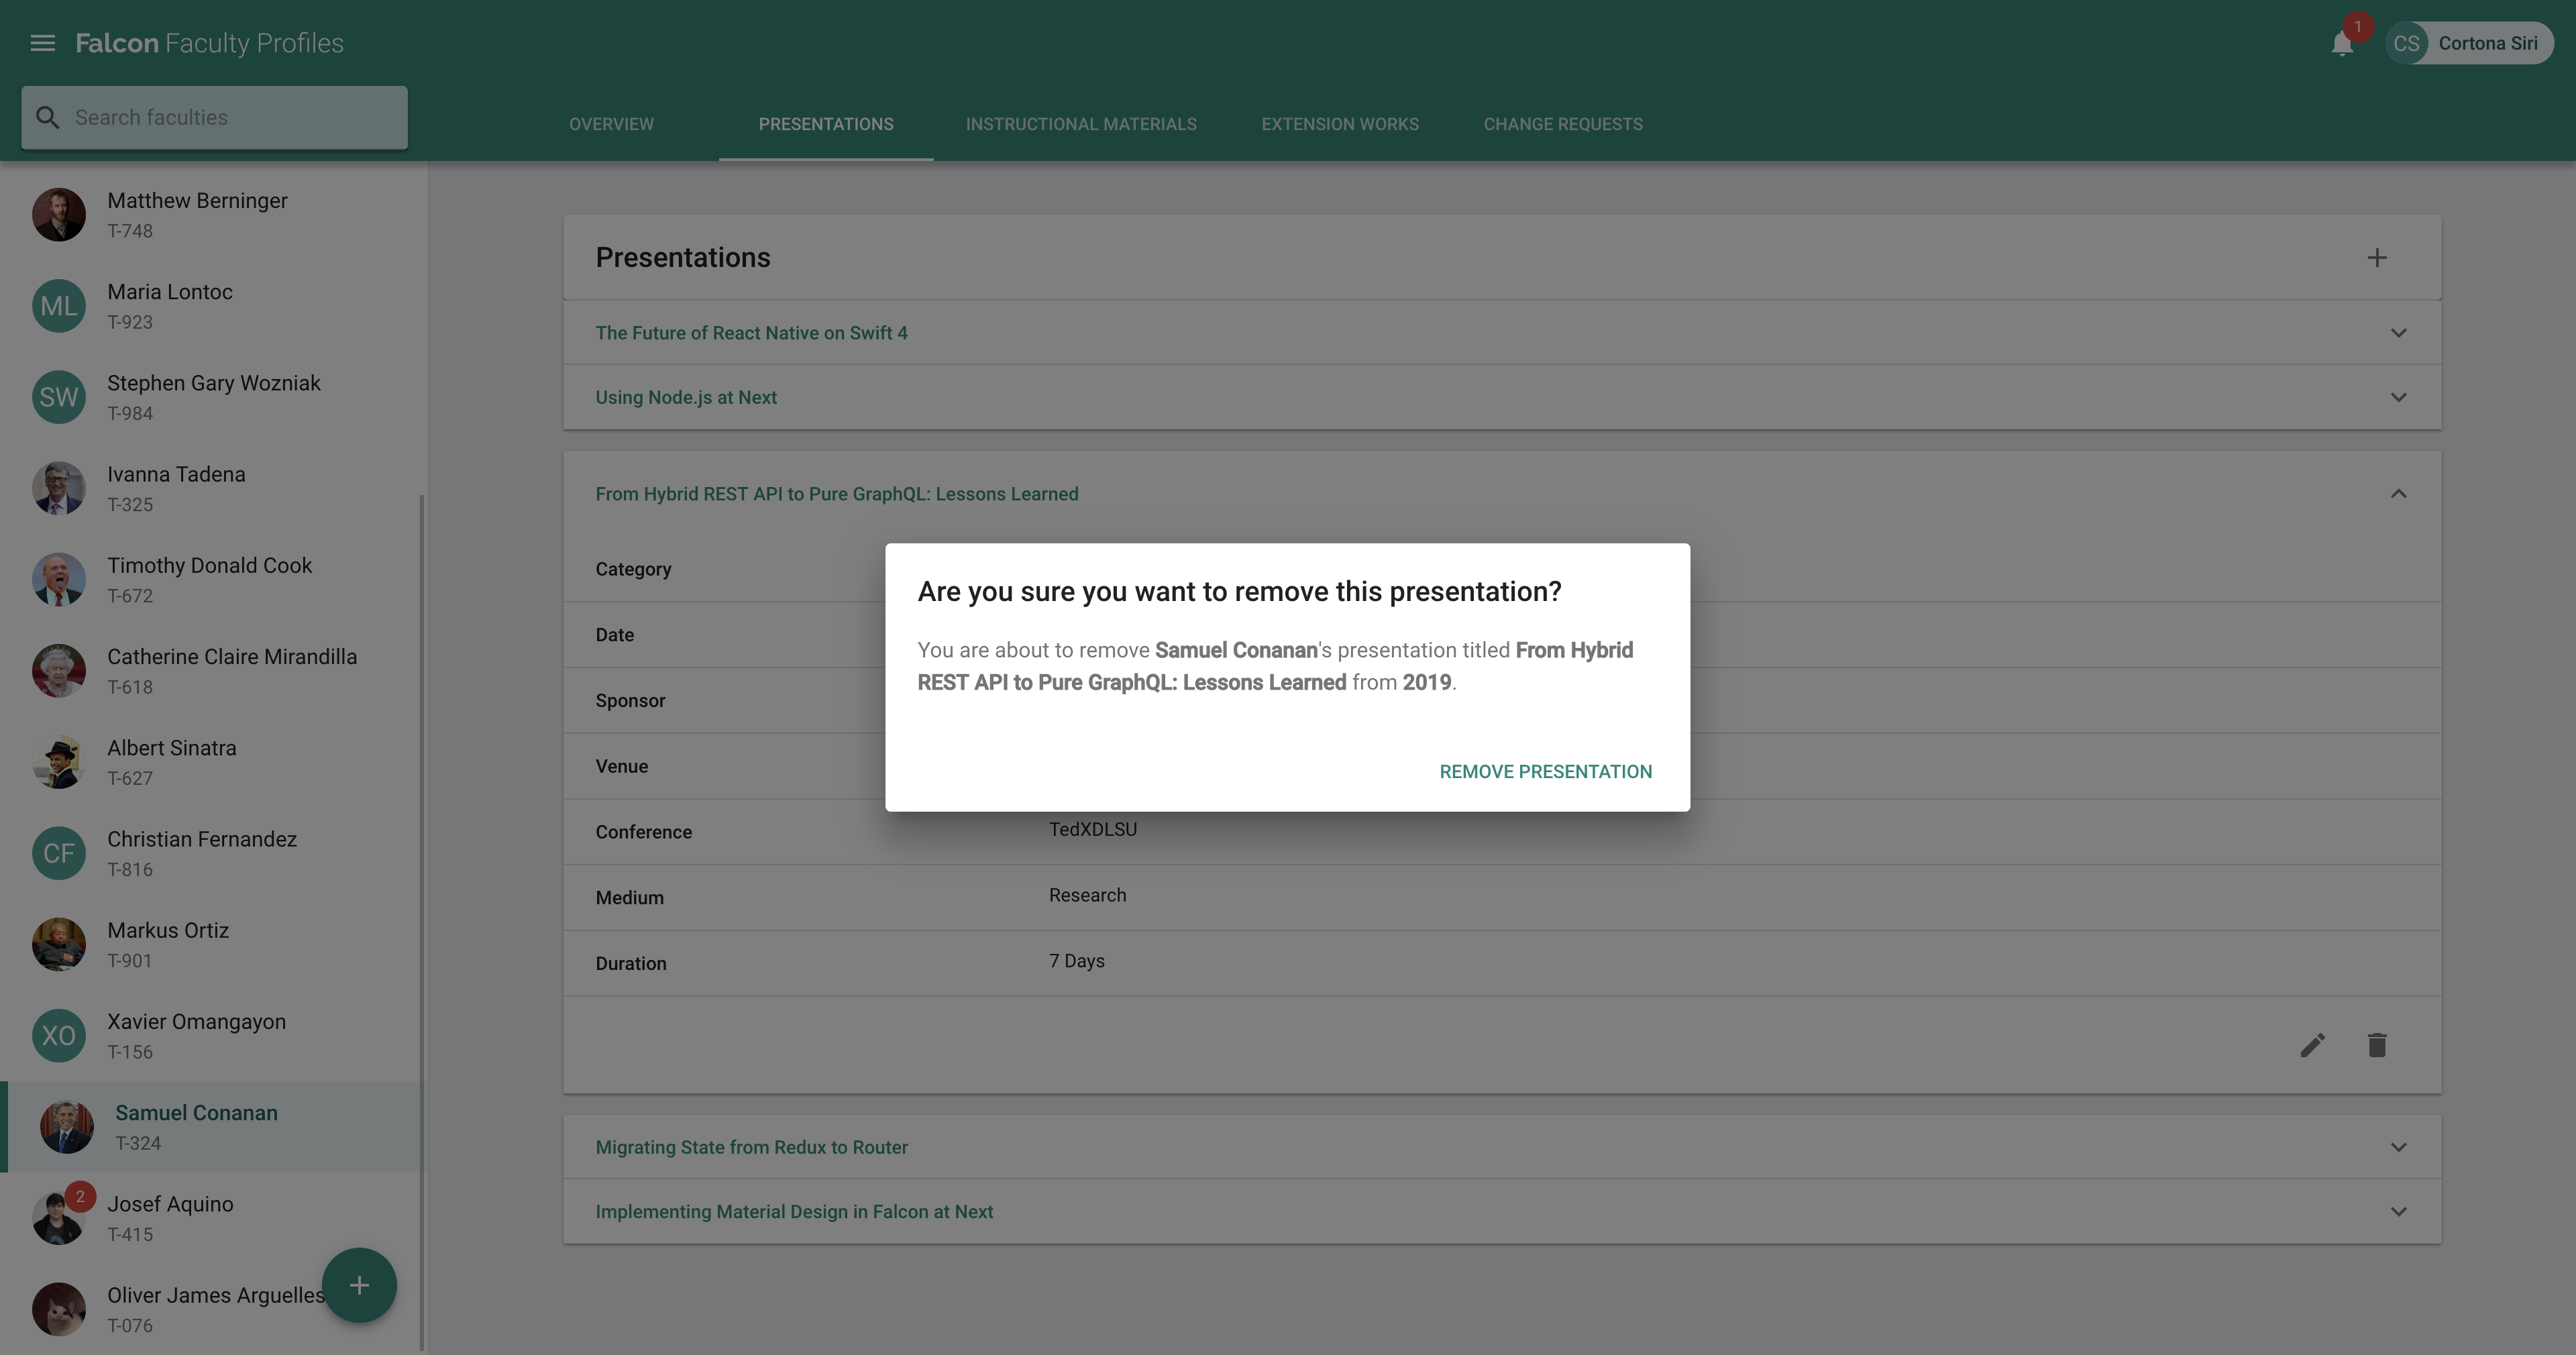
\includegraphics[width=\linewidth]{figures/screen_specifications/remove_presentation.png}
   \caption{Remove Presentations Screen}
   }
   
   \pagebreak
   
    
    \subsubsection{Instructional Materials}
    \field{Screen Name}{Instructional Materials}
    
    \field{File Name}{/pages/FacultyProfiles/components/faculty_detail_tabs/InstructionalMaterialsTab/index.js}

    \field{Description}{Displays the list of instructional materials of the faculty member and details of each instructional material. Details include the medium, audience, usage year, and student level.}
    
    \field{Layout}{}
    
\makefigure{!h}{
   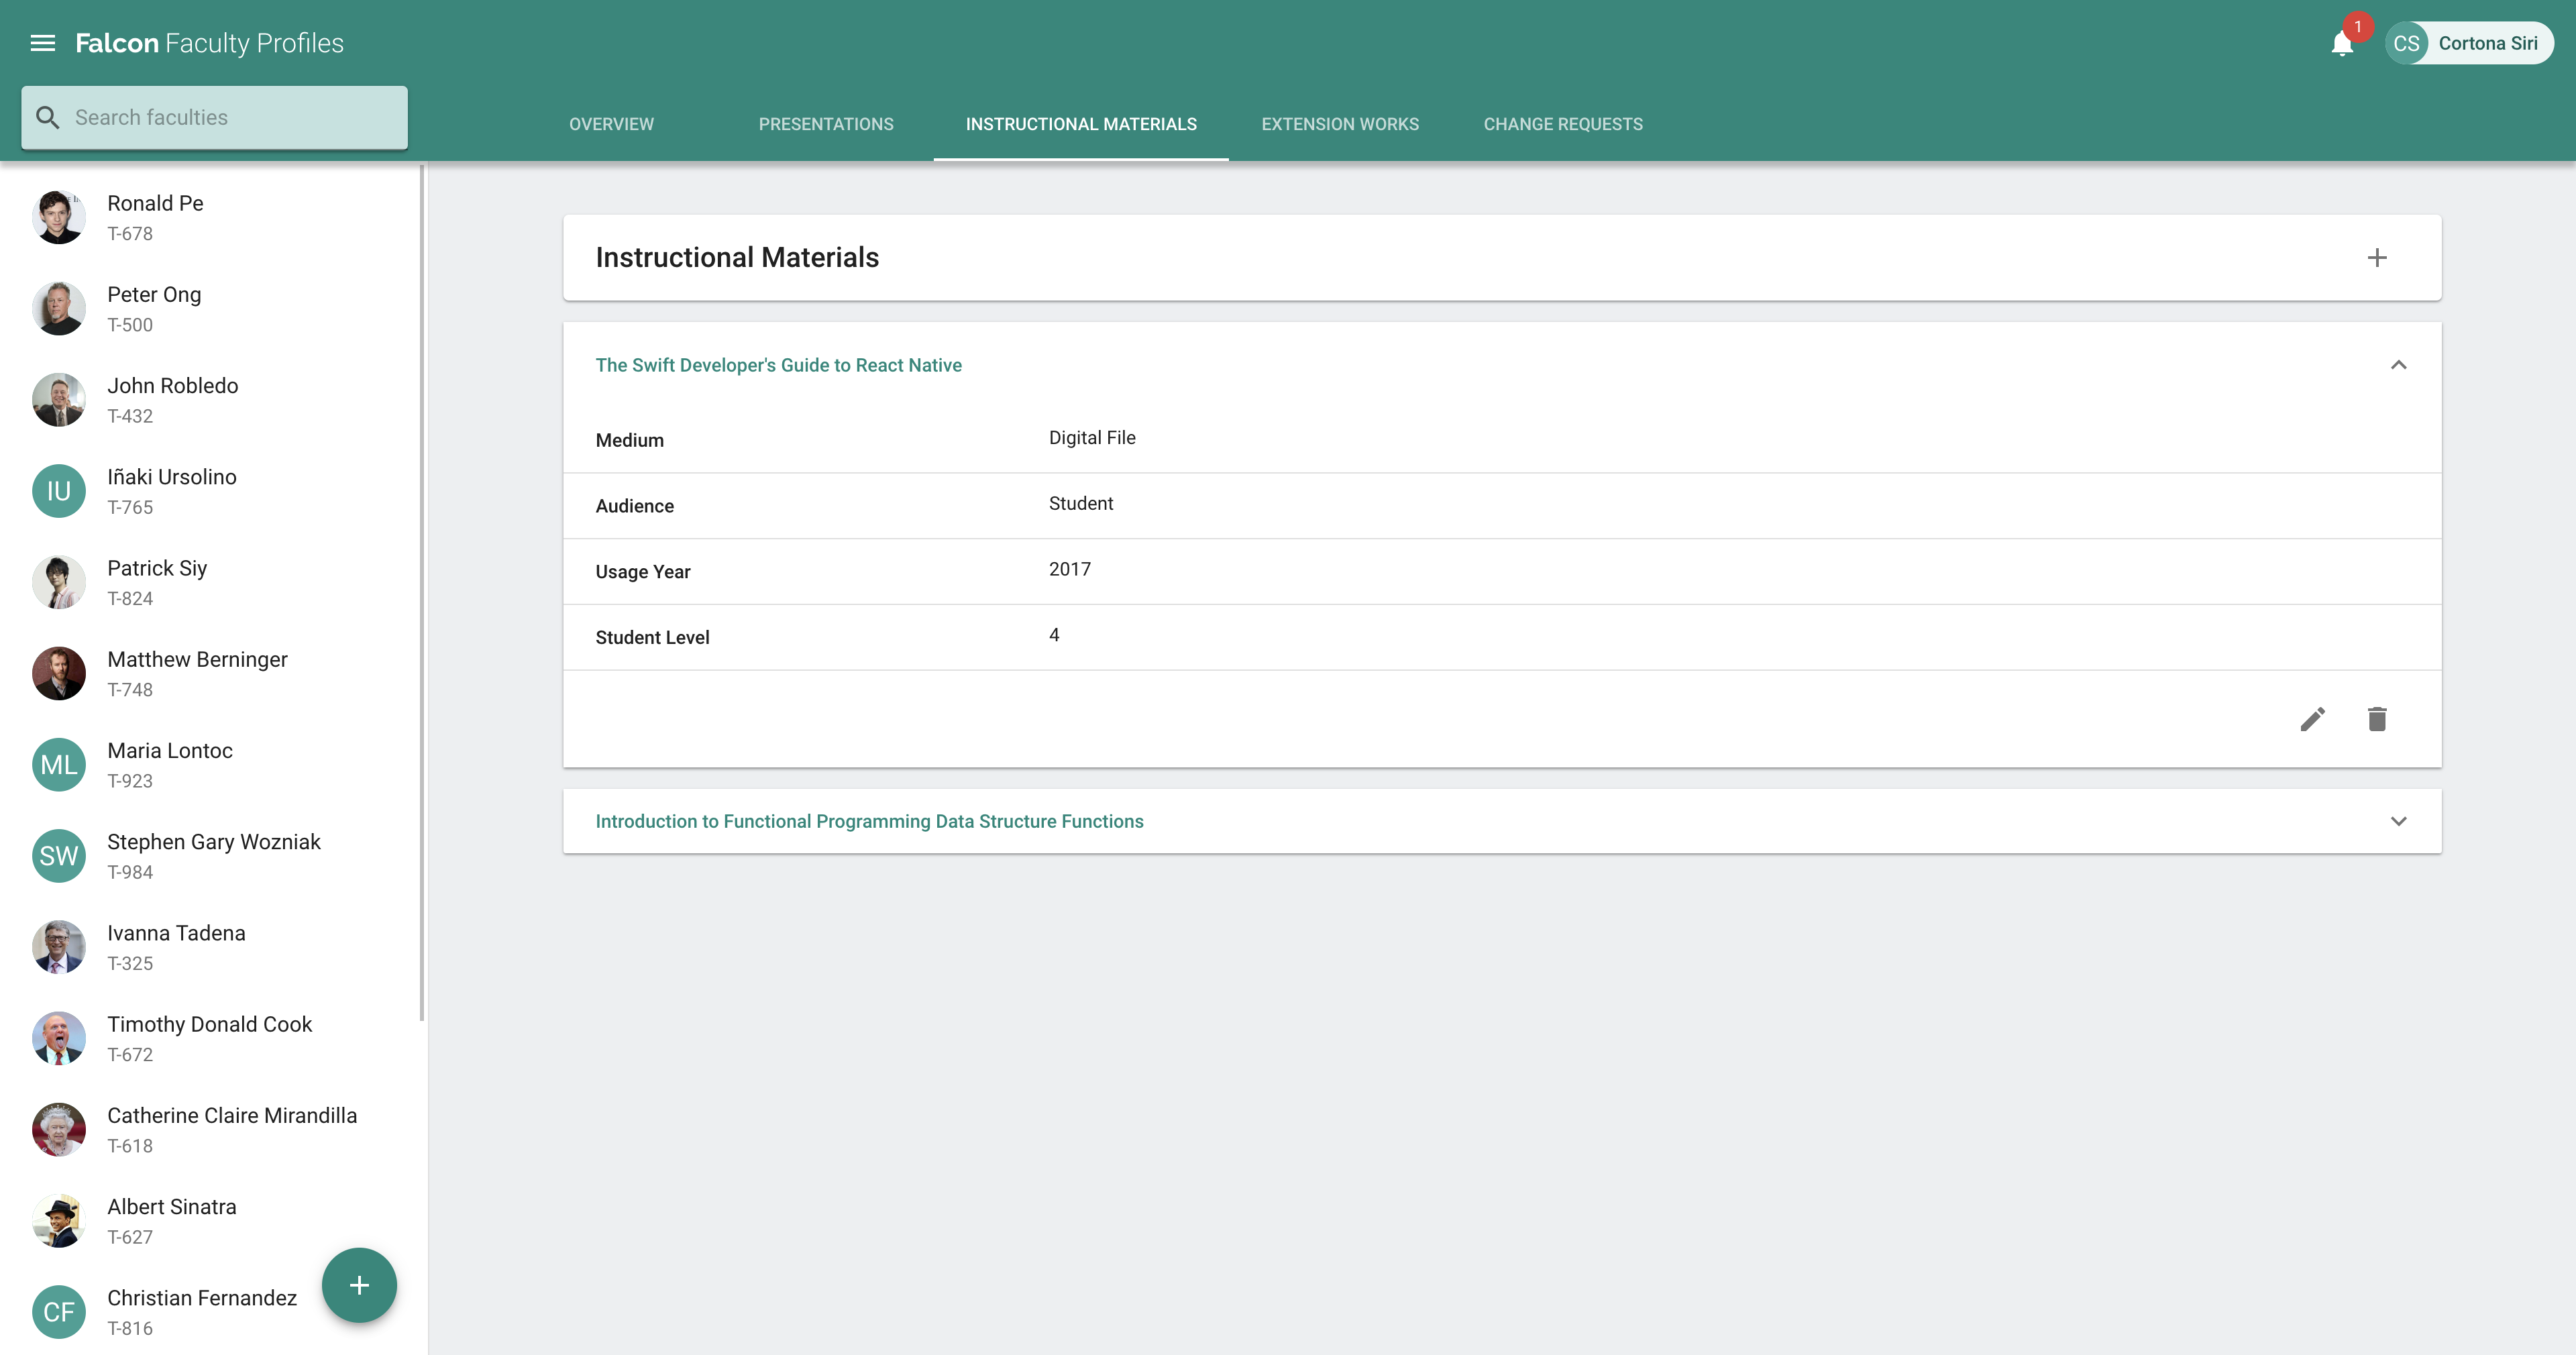
\includegraphics[width=\linewidth]{figures/screen_specifications/instructional_materials.png}
   \caption{Instructional Materials Screen}
   }
    \pagebreak

\subsubsection{Remove Instructional Materials}
    \field{Screen Name}{Remove Instructional Materials}
    
    \field{File Name}{/pages/FacultyProfiles/components/modals/RemoveInstructionalMaterialModal/index.js}

    \field{Description}{Confirm the clerk or dean if they want to remove the instructional material from the faculty profile.}
    
    \field{Layout}{}
    
\makefigure{!h}{
   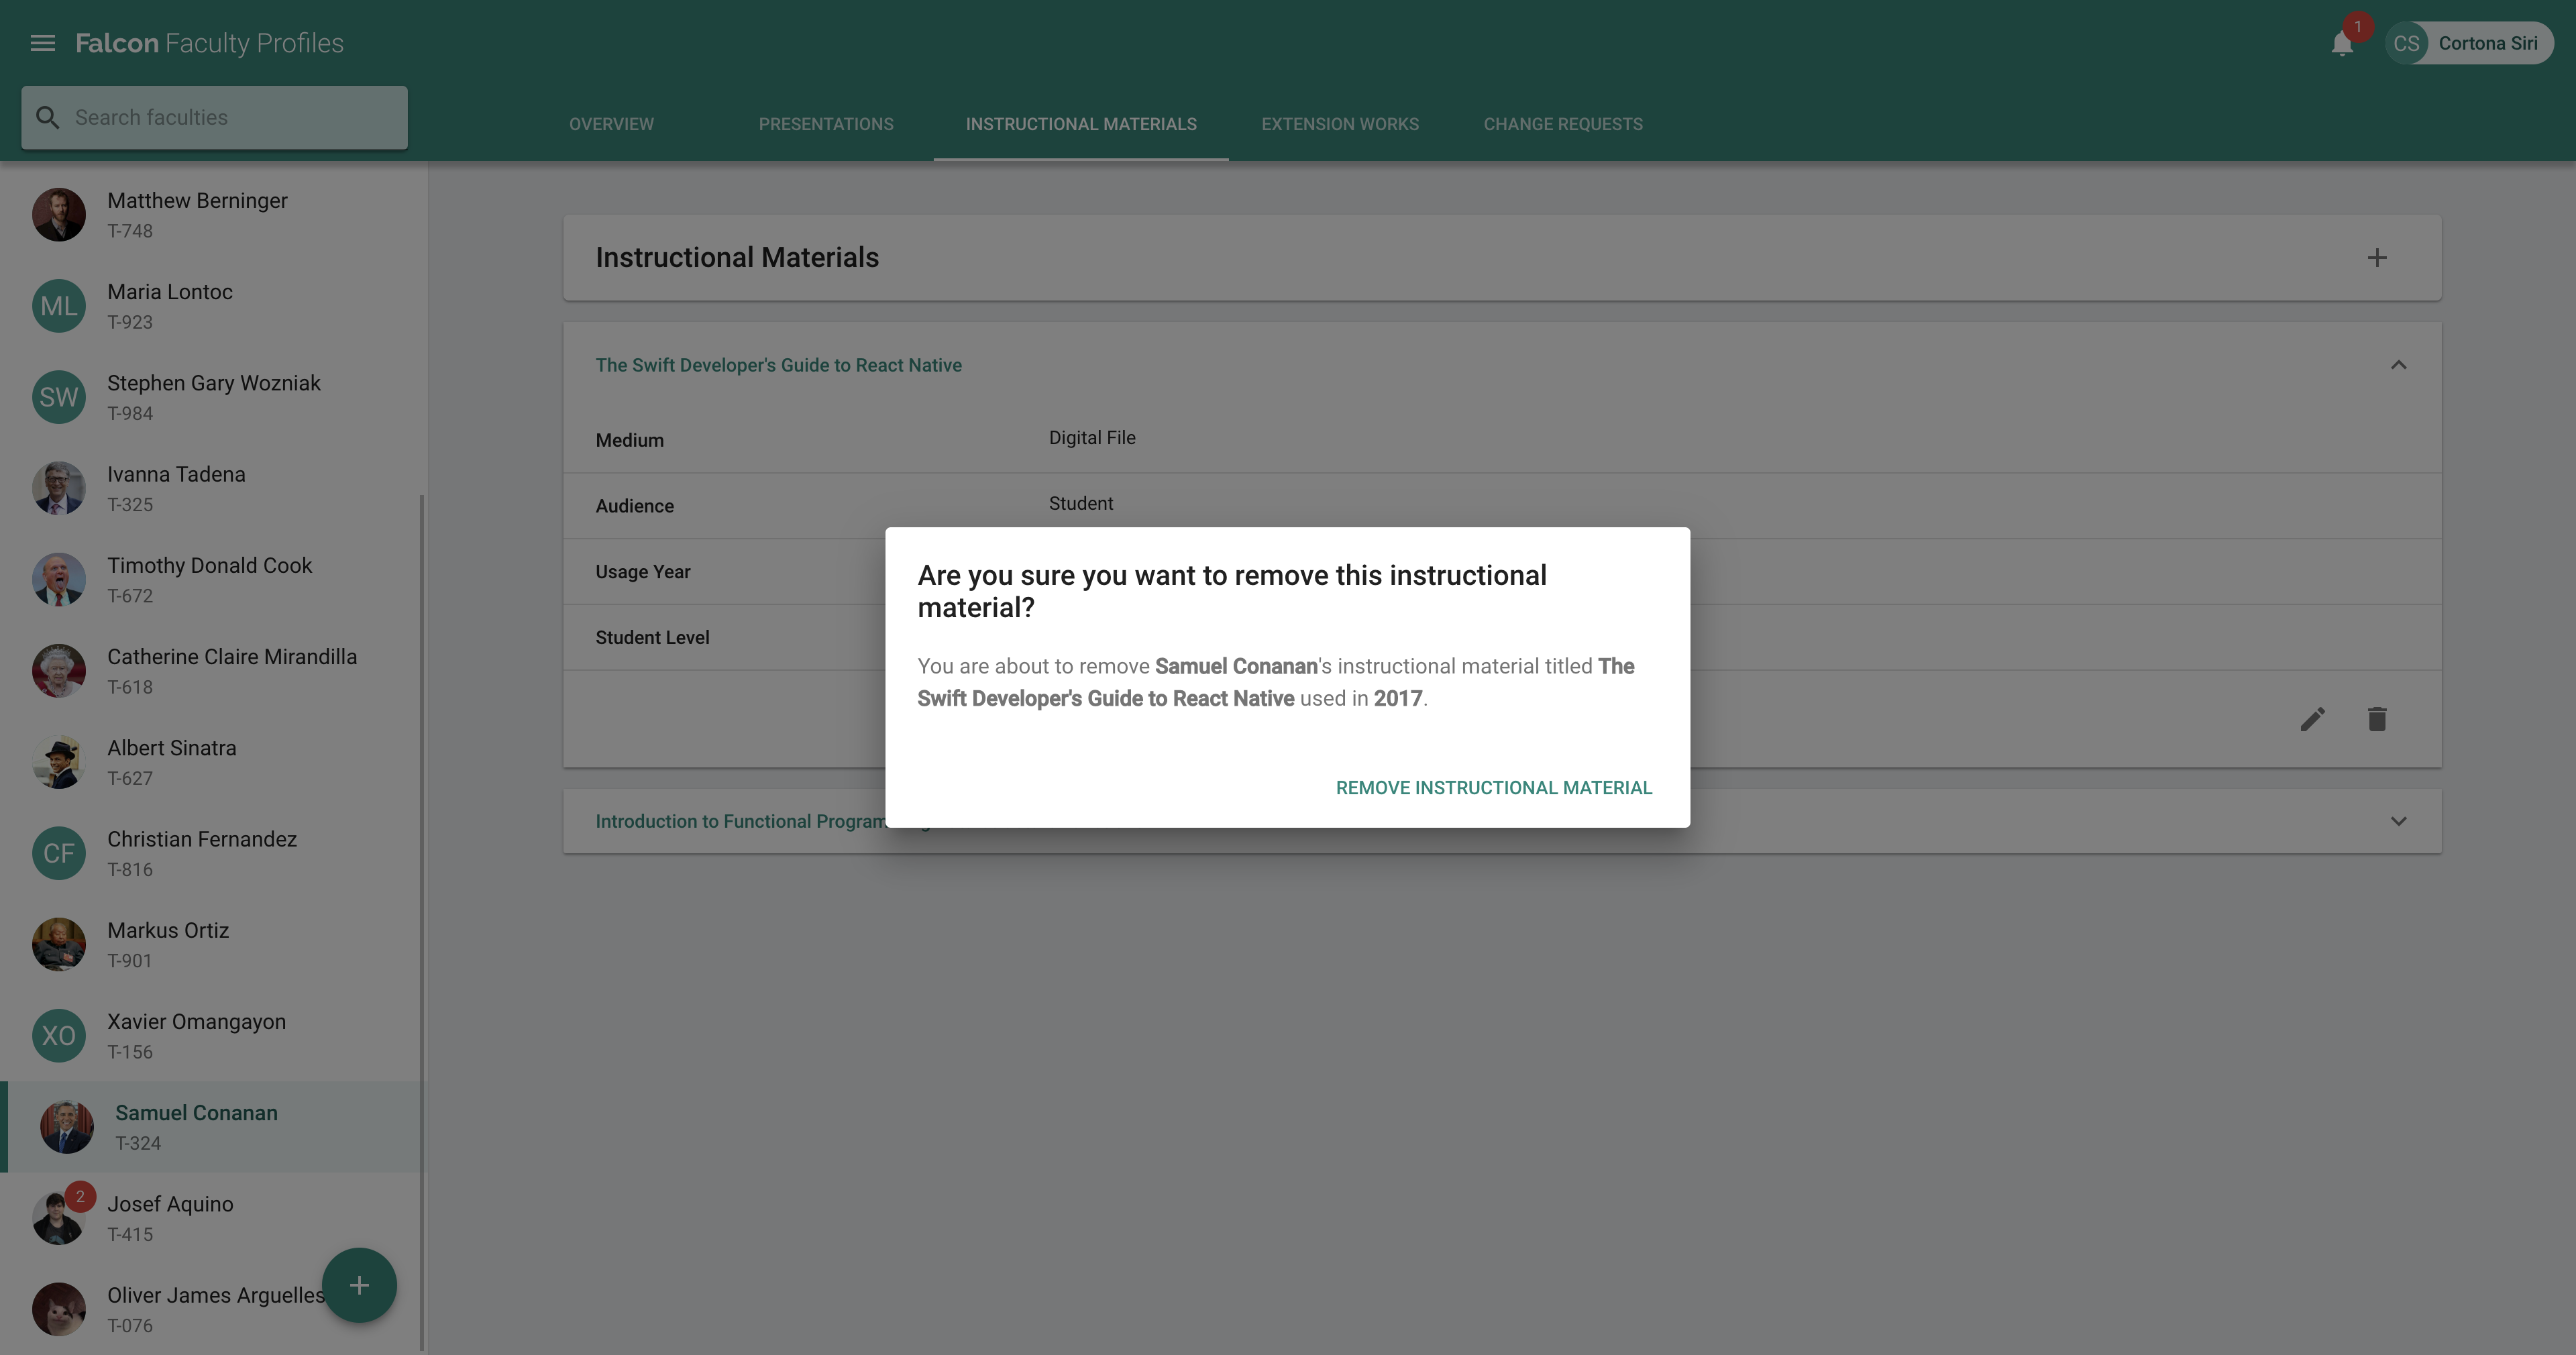
\includegraphics[width=\linewidth]{figures/screen_specifications/remove_instructional.png}
   \caption{Remove Instructional Materials Screen}
   }
    \pagebreak

    \subsubsection{Extension Works}
    \field{Screen Name}{Extension Works}
    
    \field{File Name}{/pages/FacultyProfiles/components/faculty_detail_tabs/ExtensionWorksTab/index.js}
    
    \field{Description}{Displays the list of extension works for the faculty profile with the details of each extension work. The details include the venue and roles.}
    
    \field{Layout}{} 
    
\makefigure{!h}{
   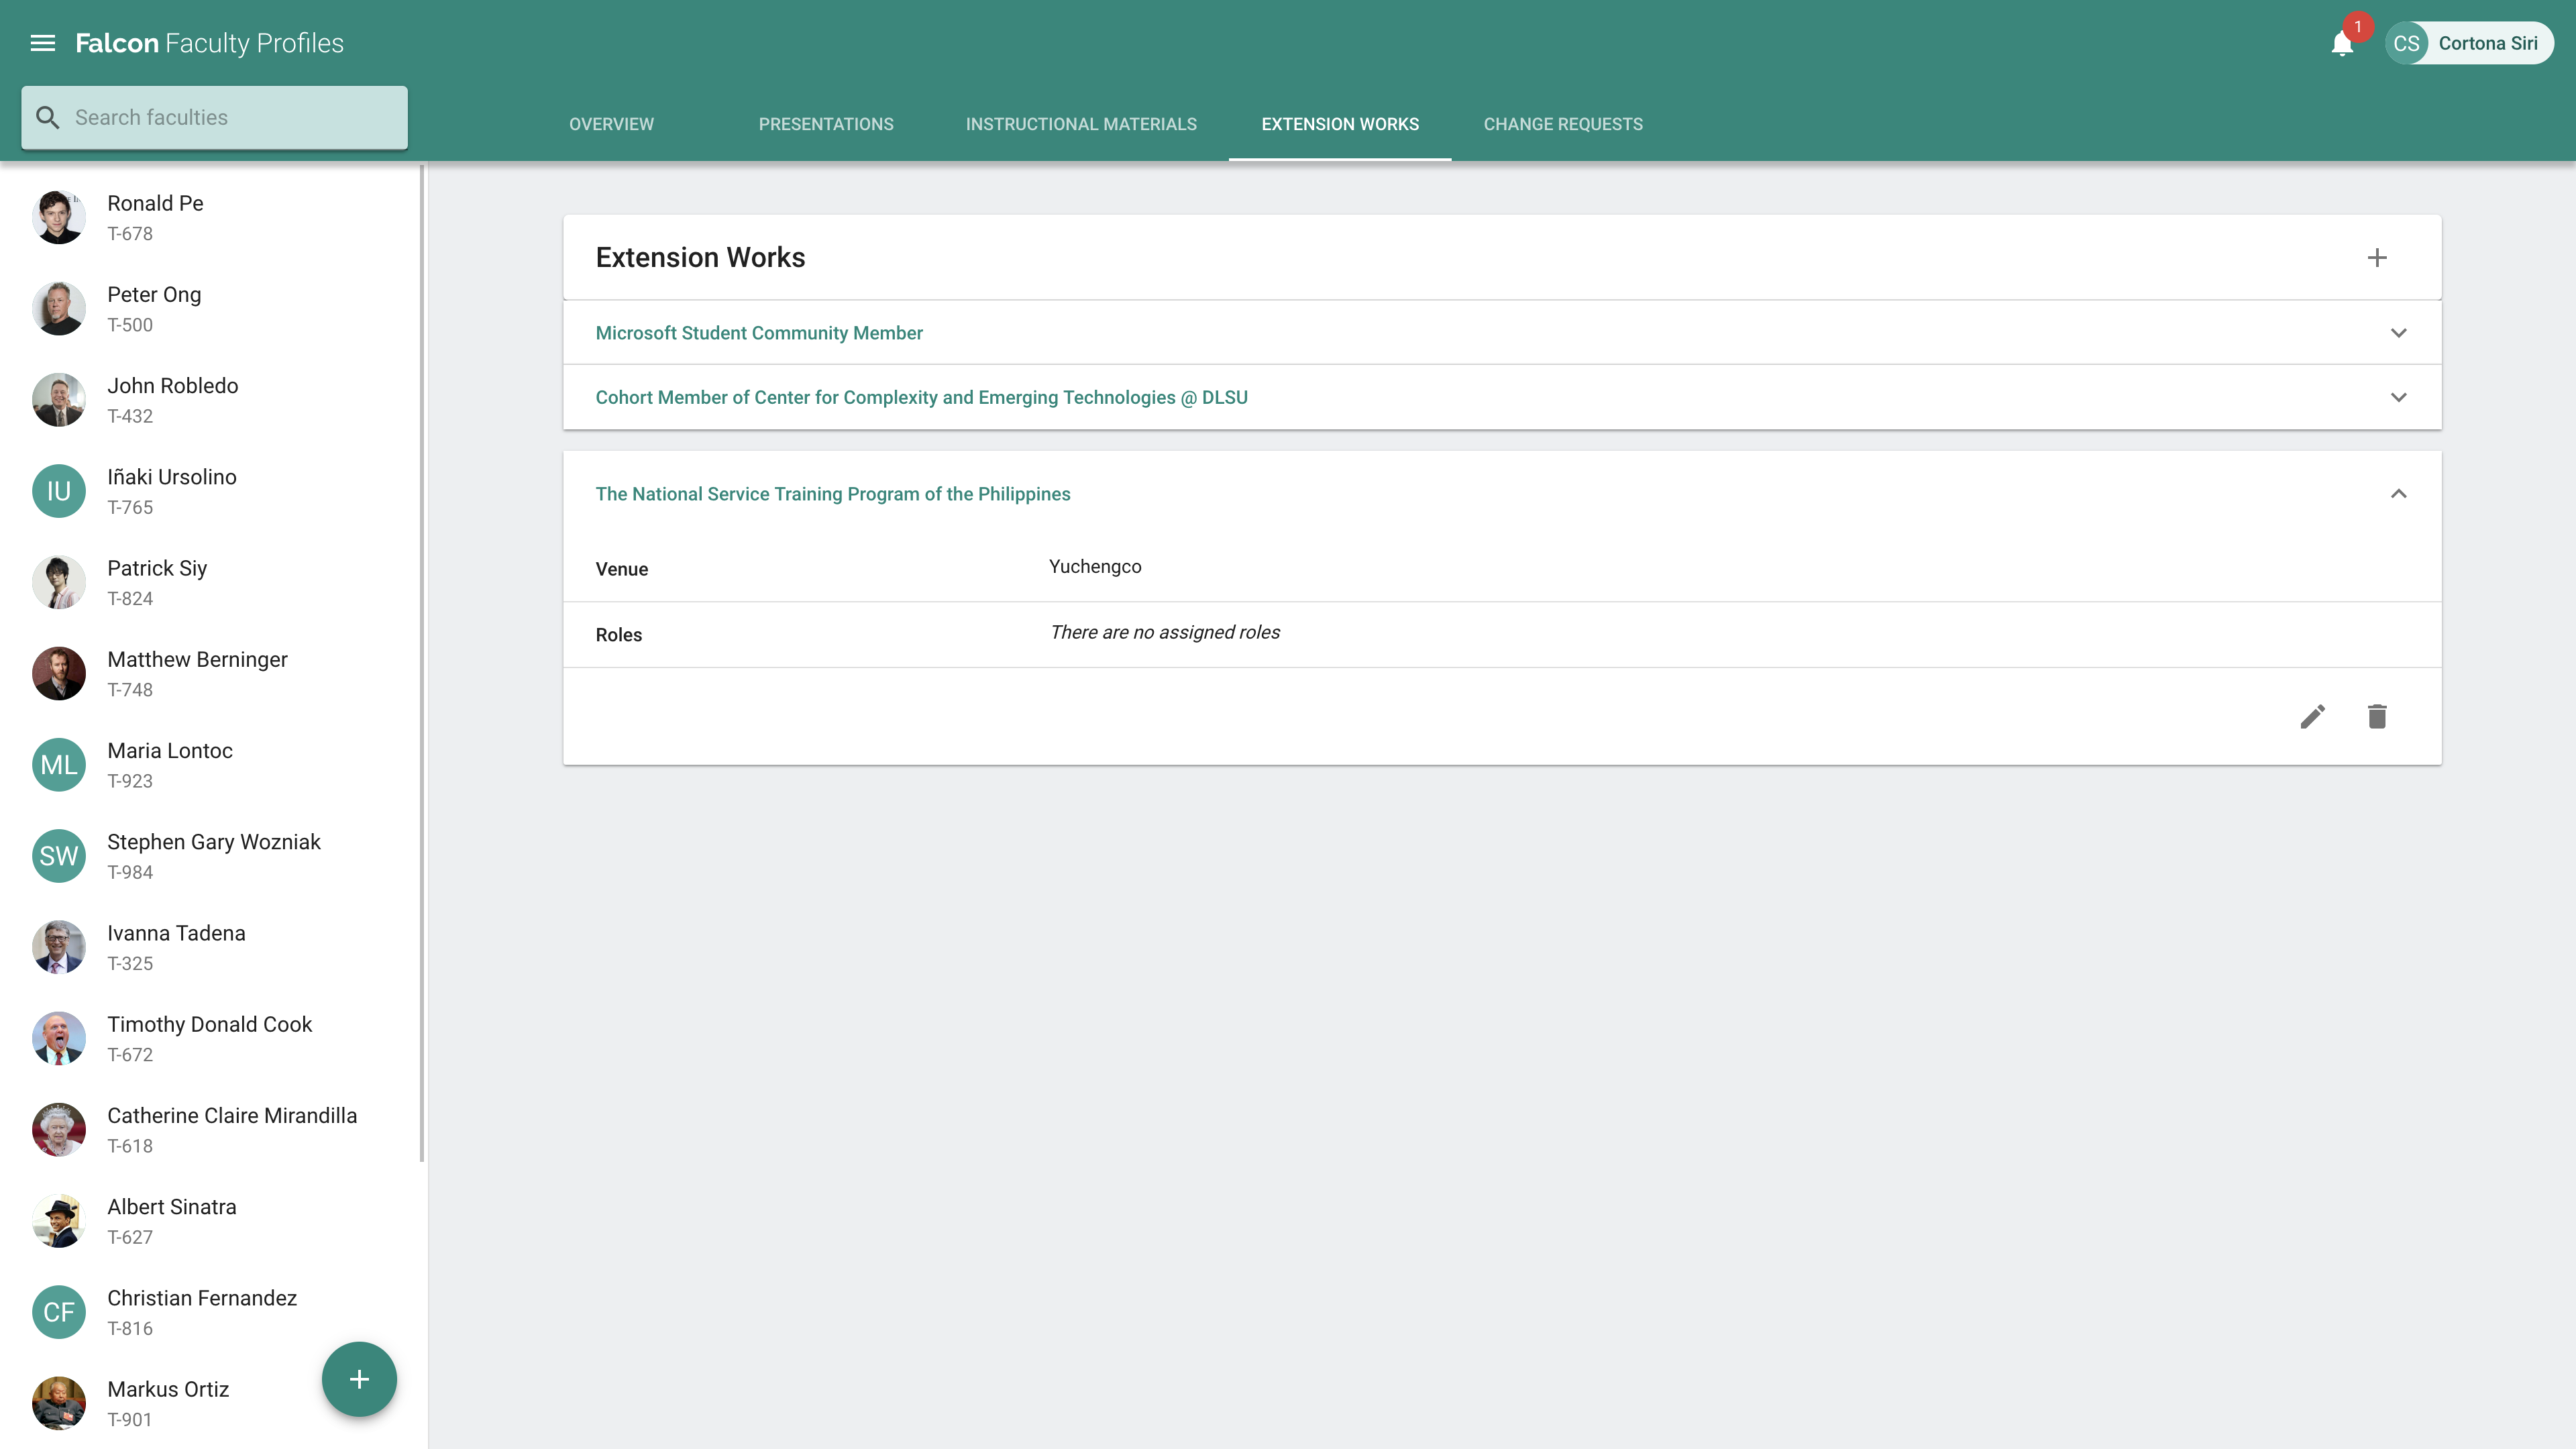
\includegraphics[width=\linewidth]{figures/screen_specifications/extension_works.png}
   \caption{Extension Works Screen}
   }
   \pagebreak
   
   \subsubsection{Remove Extension Works}
    \field{Screen Name}{Remove Extension Works}
    
    \field{File Name}{/pages/FacultyProfiles/components/modals/RemoveExtensionWorkModal/index.js}
    
    \field{Description}{To confirm the removal of an extension work from the faculty profile by the clerk or dean.}
    
    \field{Layout}{} 
    
\makefigure{!h}{
   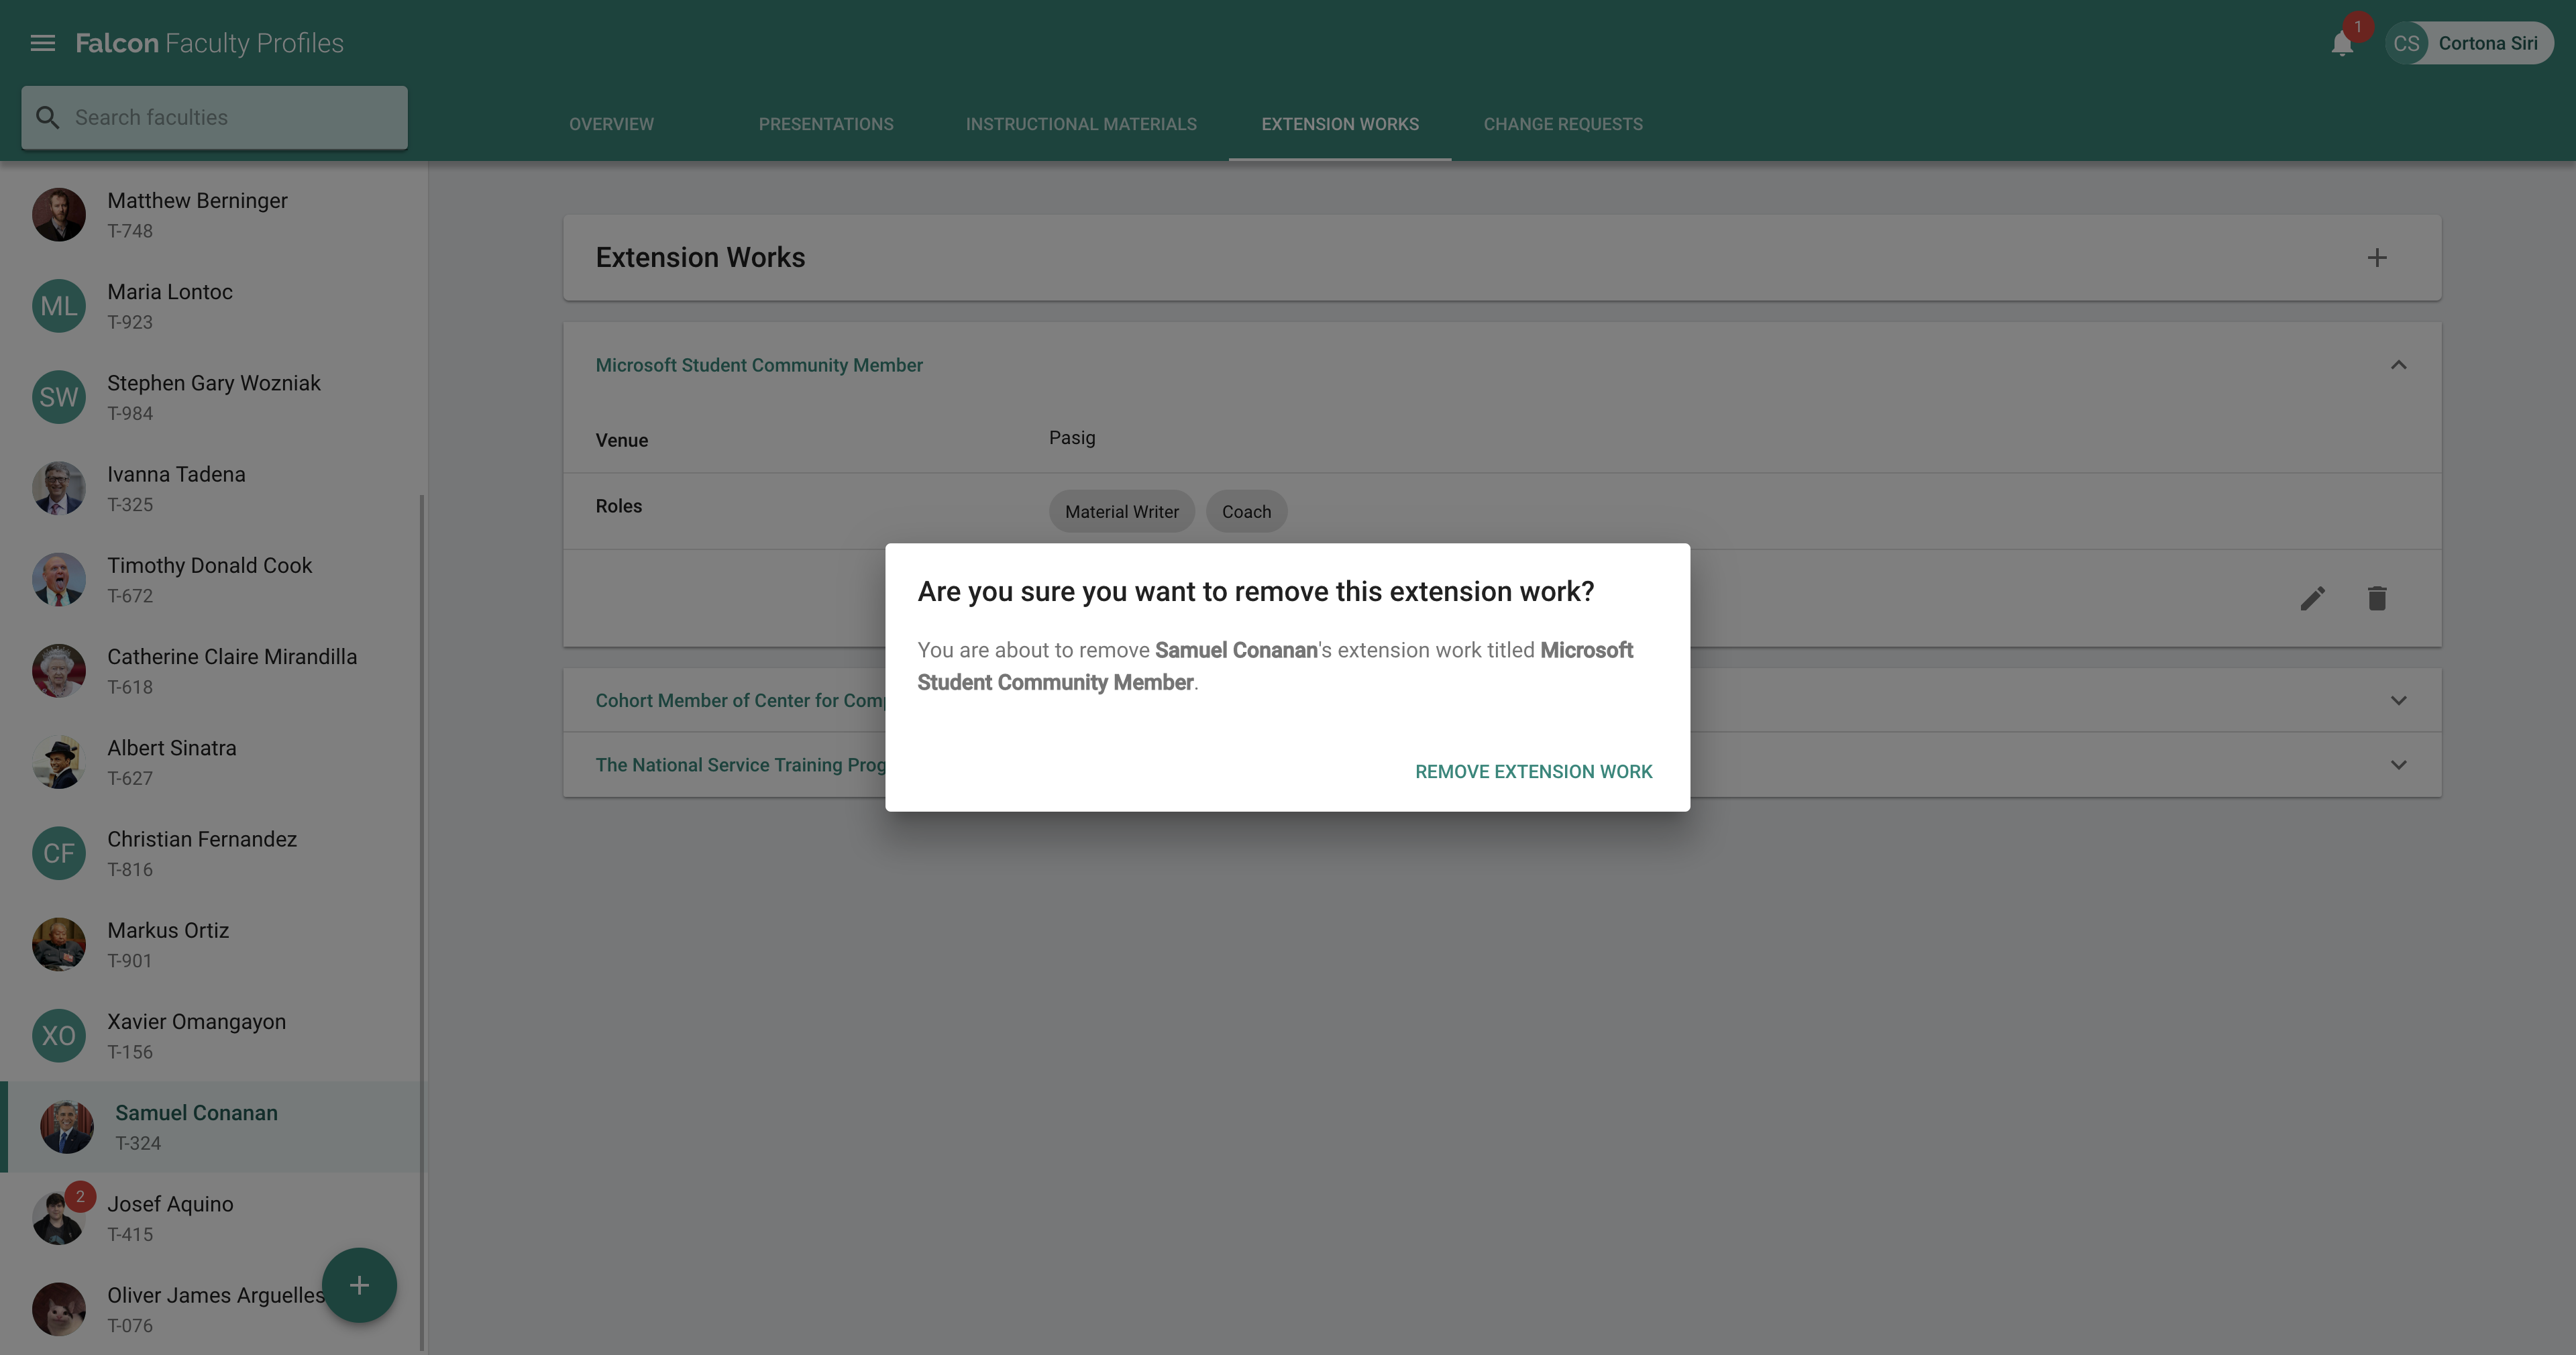
\includegraphics[width=\linewidth]{figures/screen_specifications/remove_extension.png}
   \caption{Remove Extension Works Screen}
   }
   \pagebreak
   
    \subsubsection{Notifications}
    
    \field{Screen Name}{Notifications}
    
    \field{File Name}{/pages/App/components/notifications/NotificationsButton/index.js}
    
    \field{Description} {Notifies the user of any updates and shows the list of notifications.}
    
    \field{Layout}{}
    
\makefigure{!h}{
   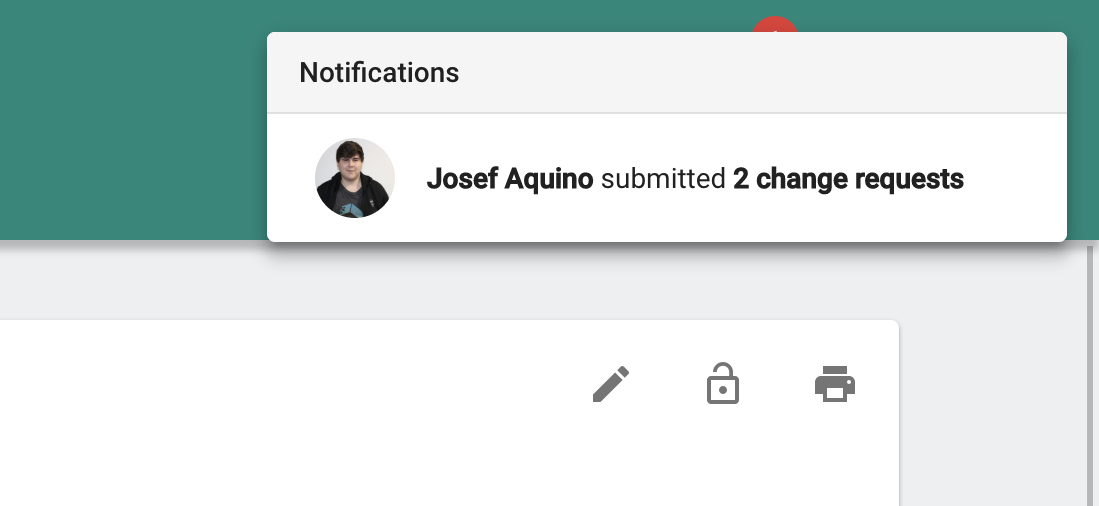
\includegraphics[width=\linewidth]{figures/screen_specifications/notifications.png}
   \caption{Notifications Screen}
   }
   
\pagebreak
   
   \subsubsection{Change Requests}
    
    \field{Screen Name}{Change Requests}
    
    \field{File Name}{/pages/FacultyProfiles/components/faculty_detail_tabs/ChangeRequestsTab/index.js}
    
    \field{Description} {Displays the list of change requests of the faculty members with details.}
    
    \field{Layout}{}
    
\makefigure{!h}{
   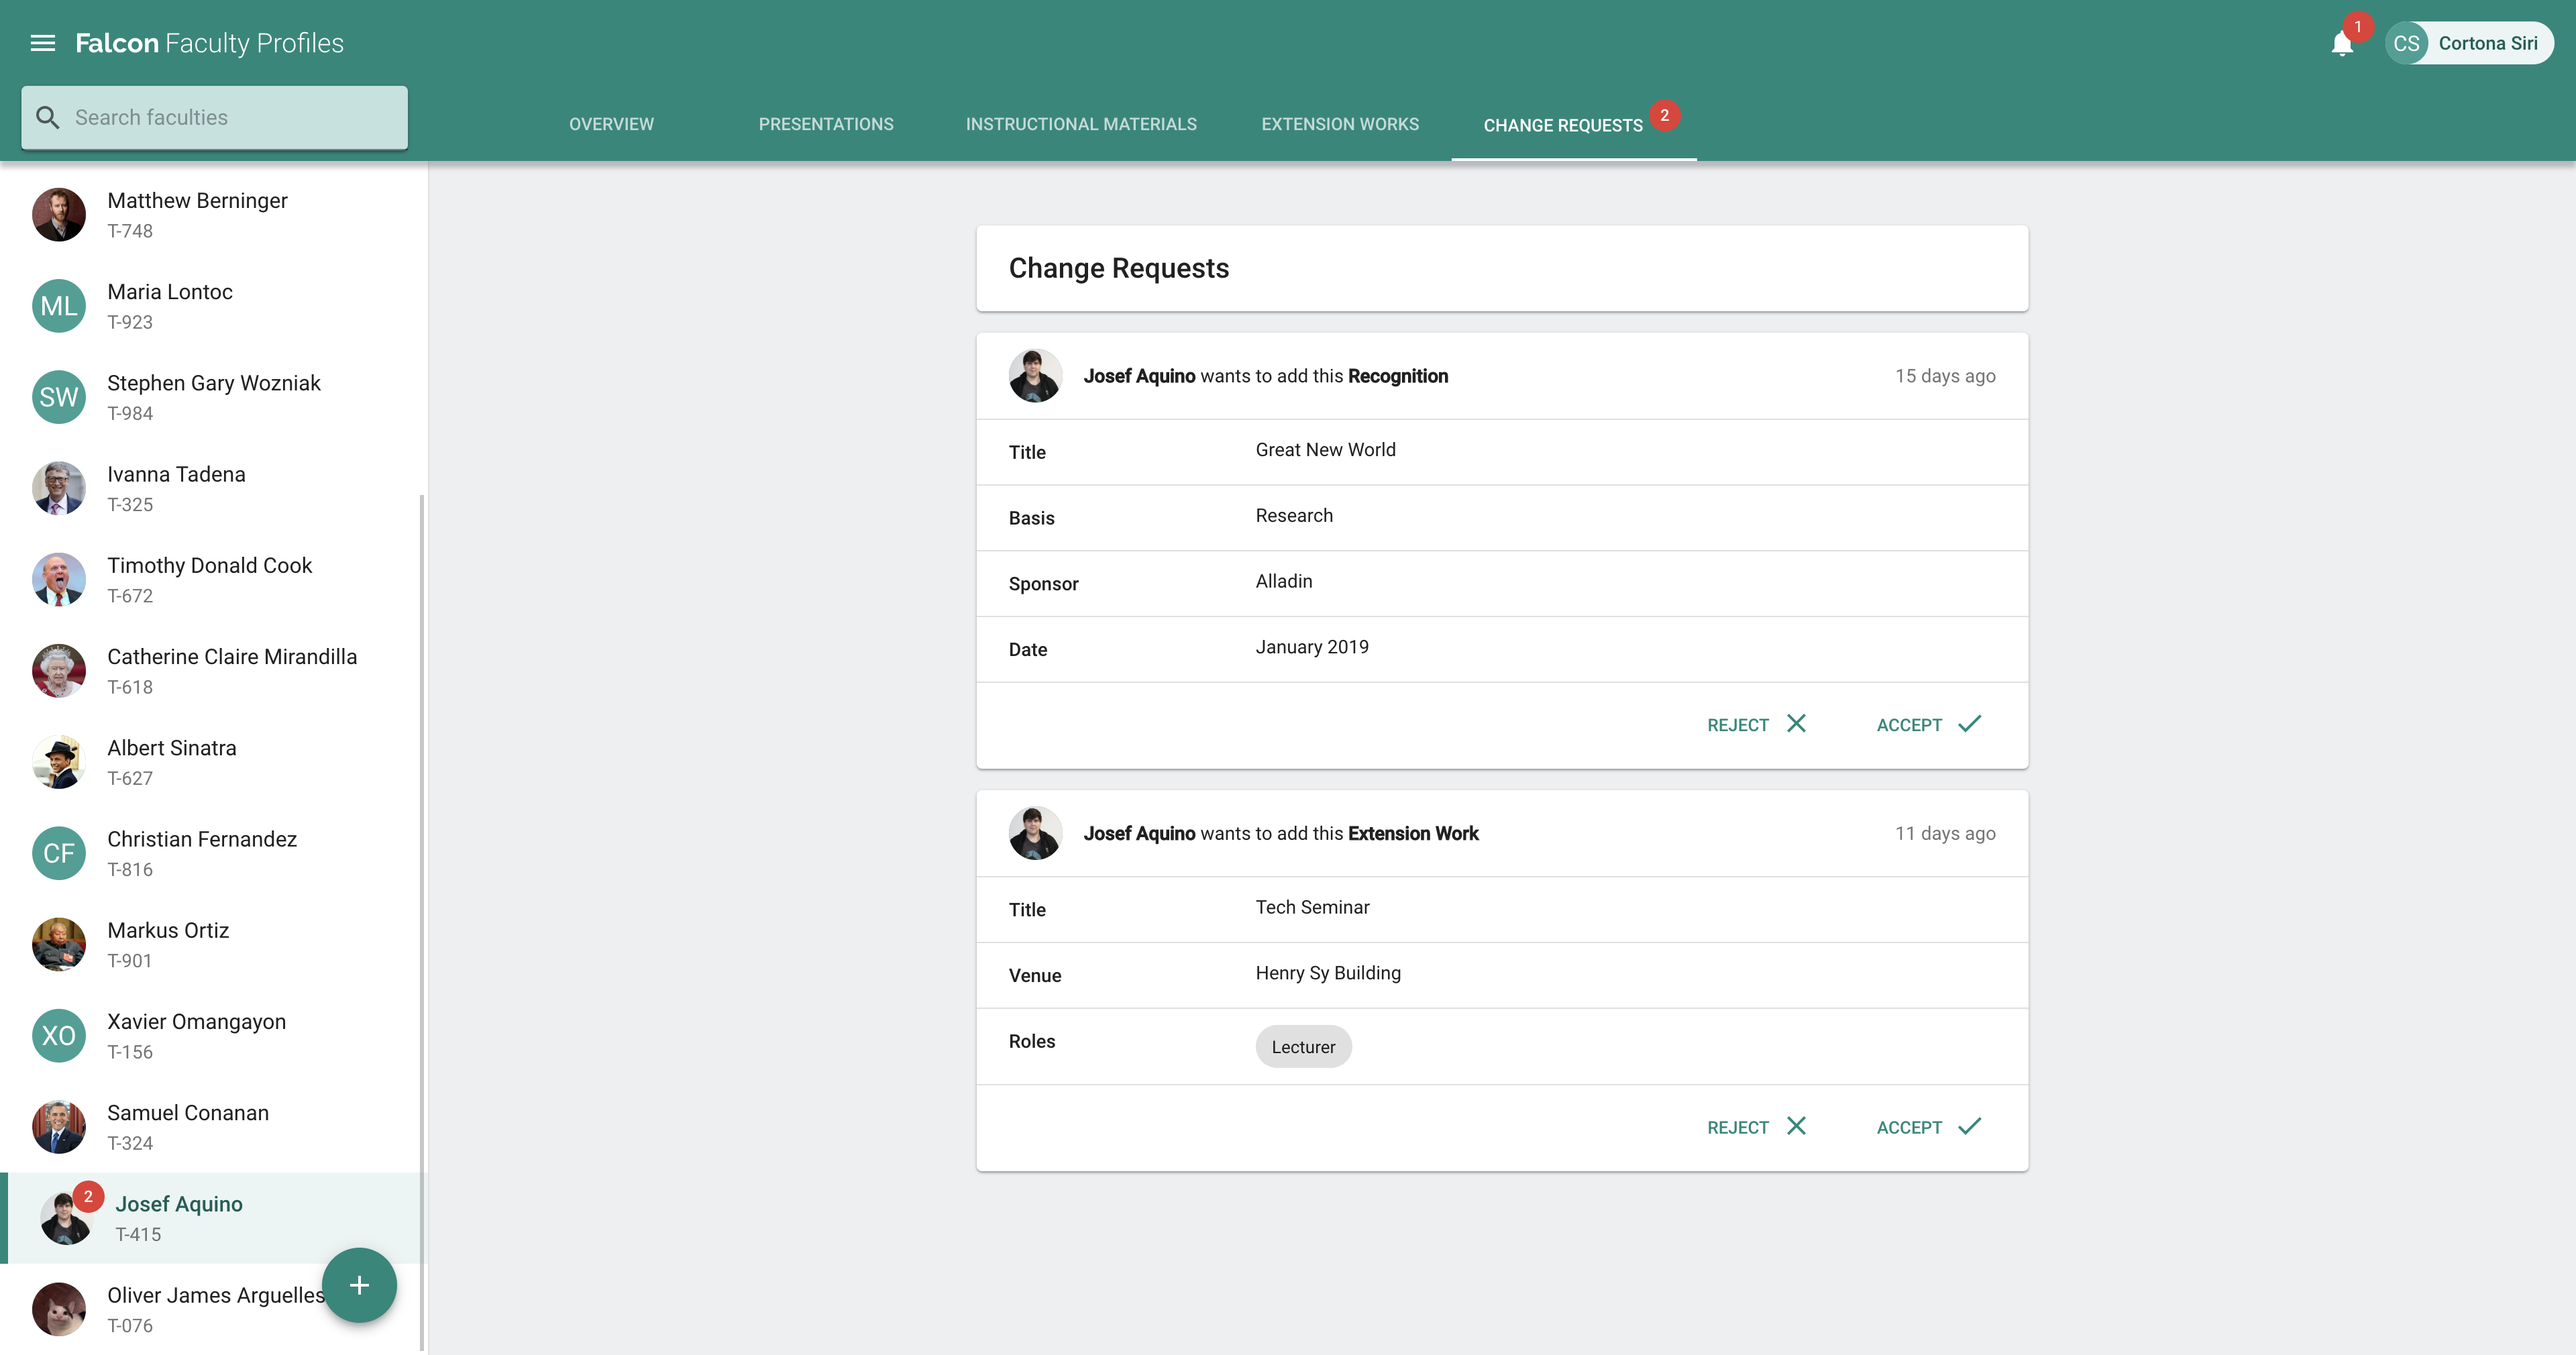
\includegraphics[width=\linewidth]{figures/screen_specifications/change_requests.png}
   \caption{Change Requests Screen}
   }
   
   \pagebreak
   
   \subsection{My Profile}
   
   \subsubsection{My Profile Overview}
    
    \field{Screen Name}{My Profile Overview}
    
    \field{File Name}{/pages/MyProfile/index.js}
    
    \field{Description} {Displays the details of the faculty profile. The first card displays the basic information, second displays the expertise of the faculty member, third card displays the degrees, and the fourth displays the recognitions.}
    
    \field{Layout}{}
    
\makefigure{!h}{
   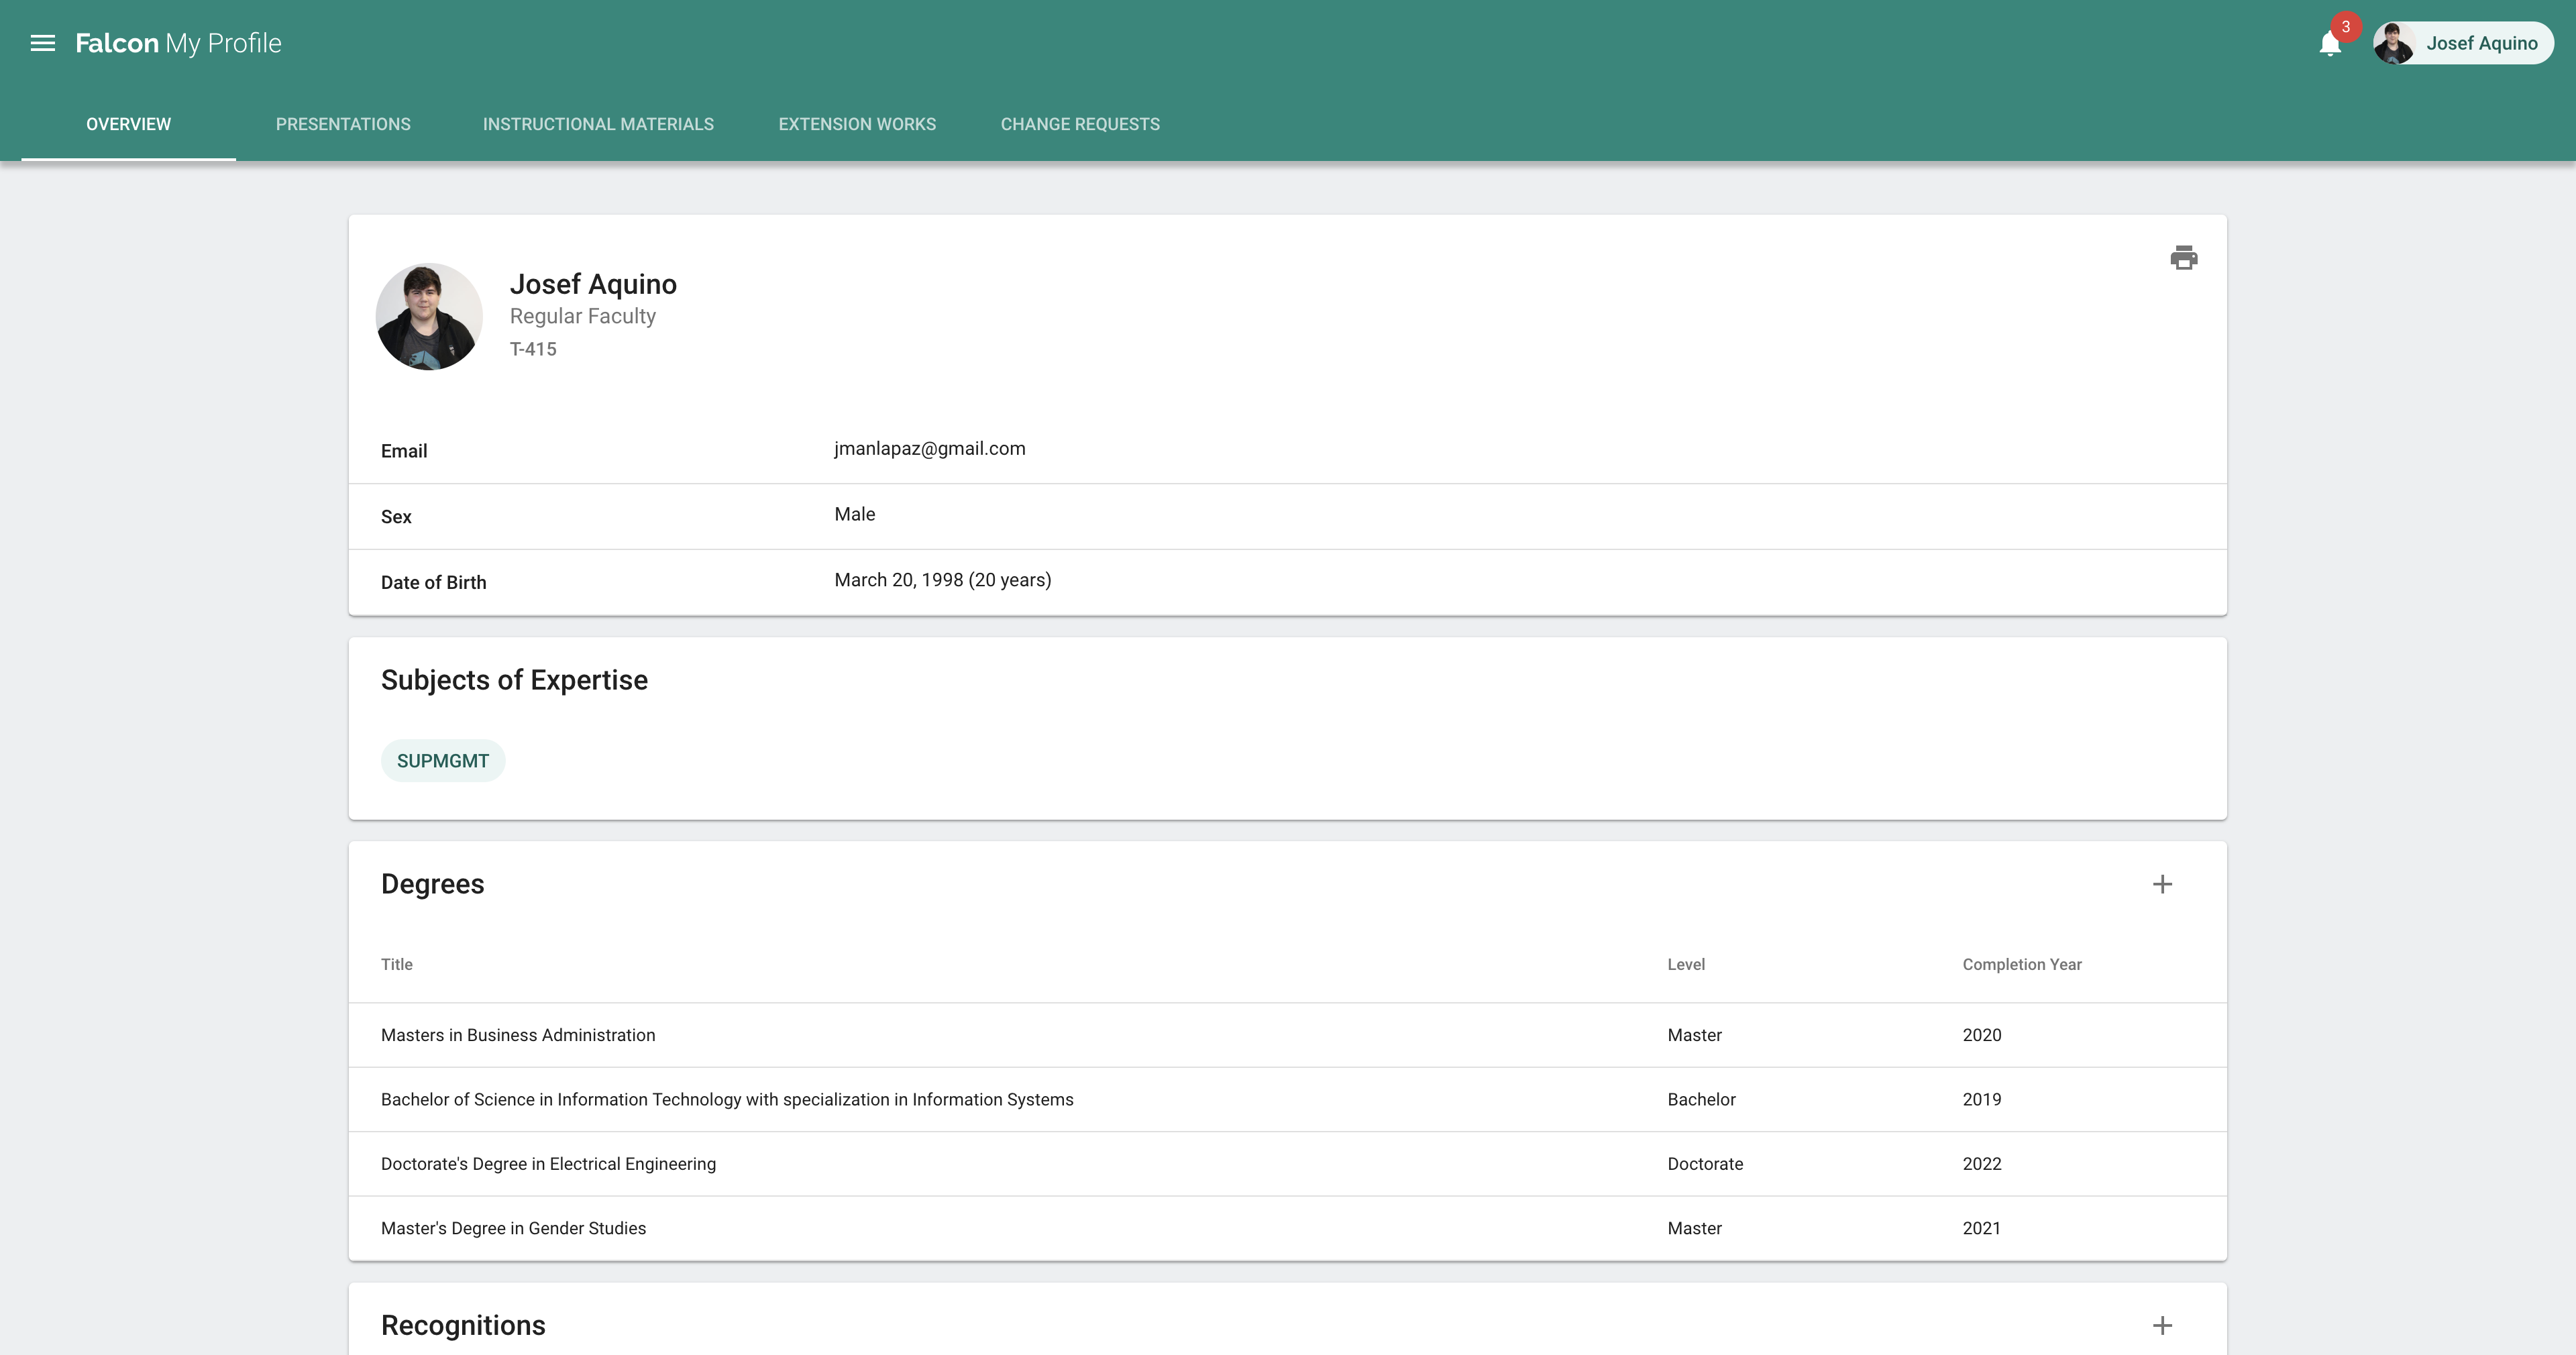
\includegraphics[width=\linewidth]{figures/screen_specifications/myprofile_screens/my_profileA.png}
   \caption{My Profile Overview Screen A}
   }
   
   \pagebreak
   
\makefigure{!h}{
   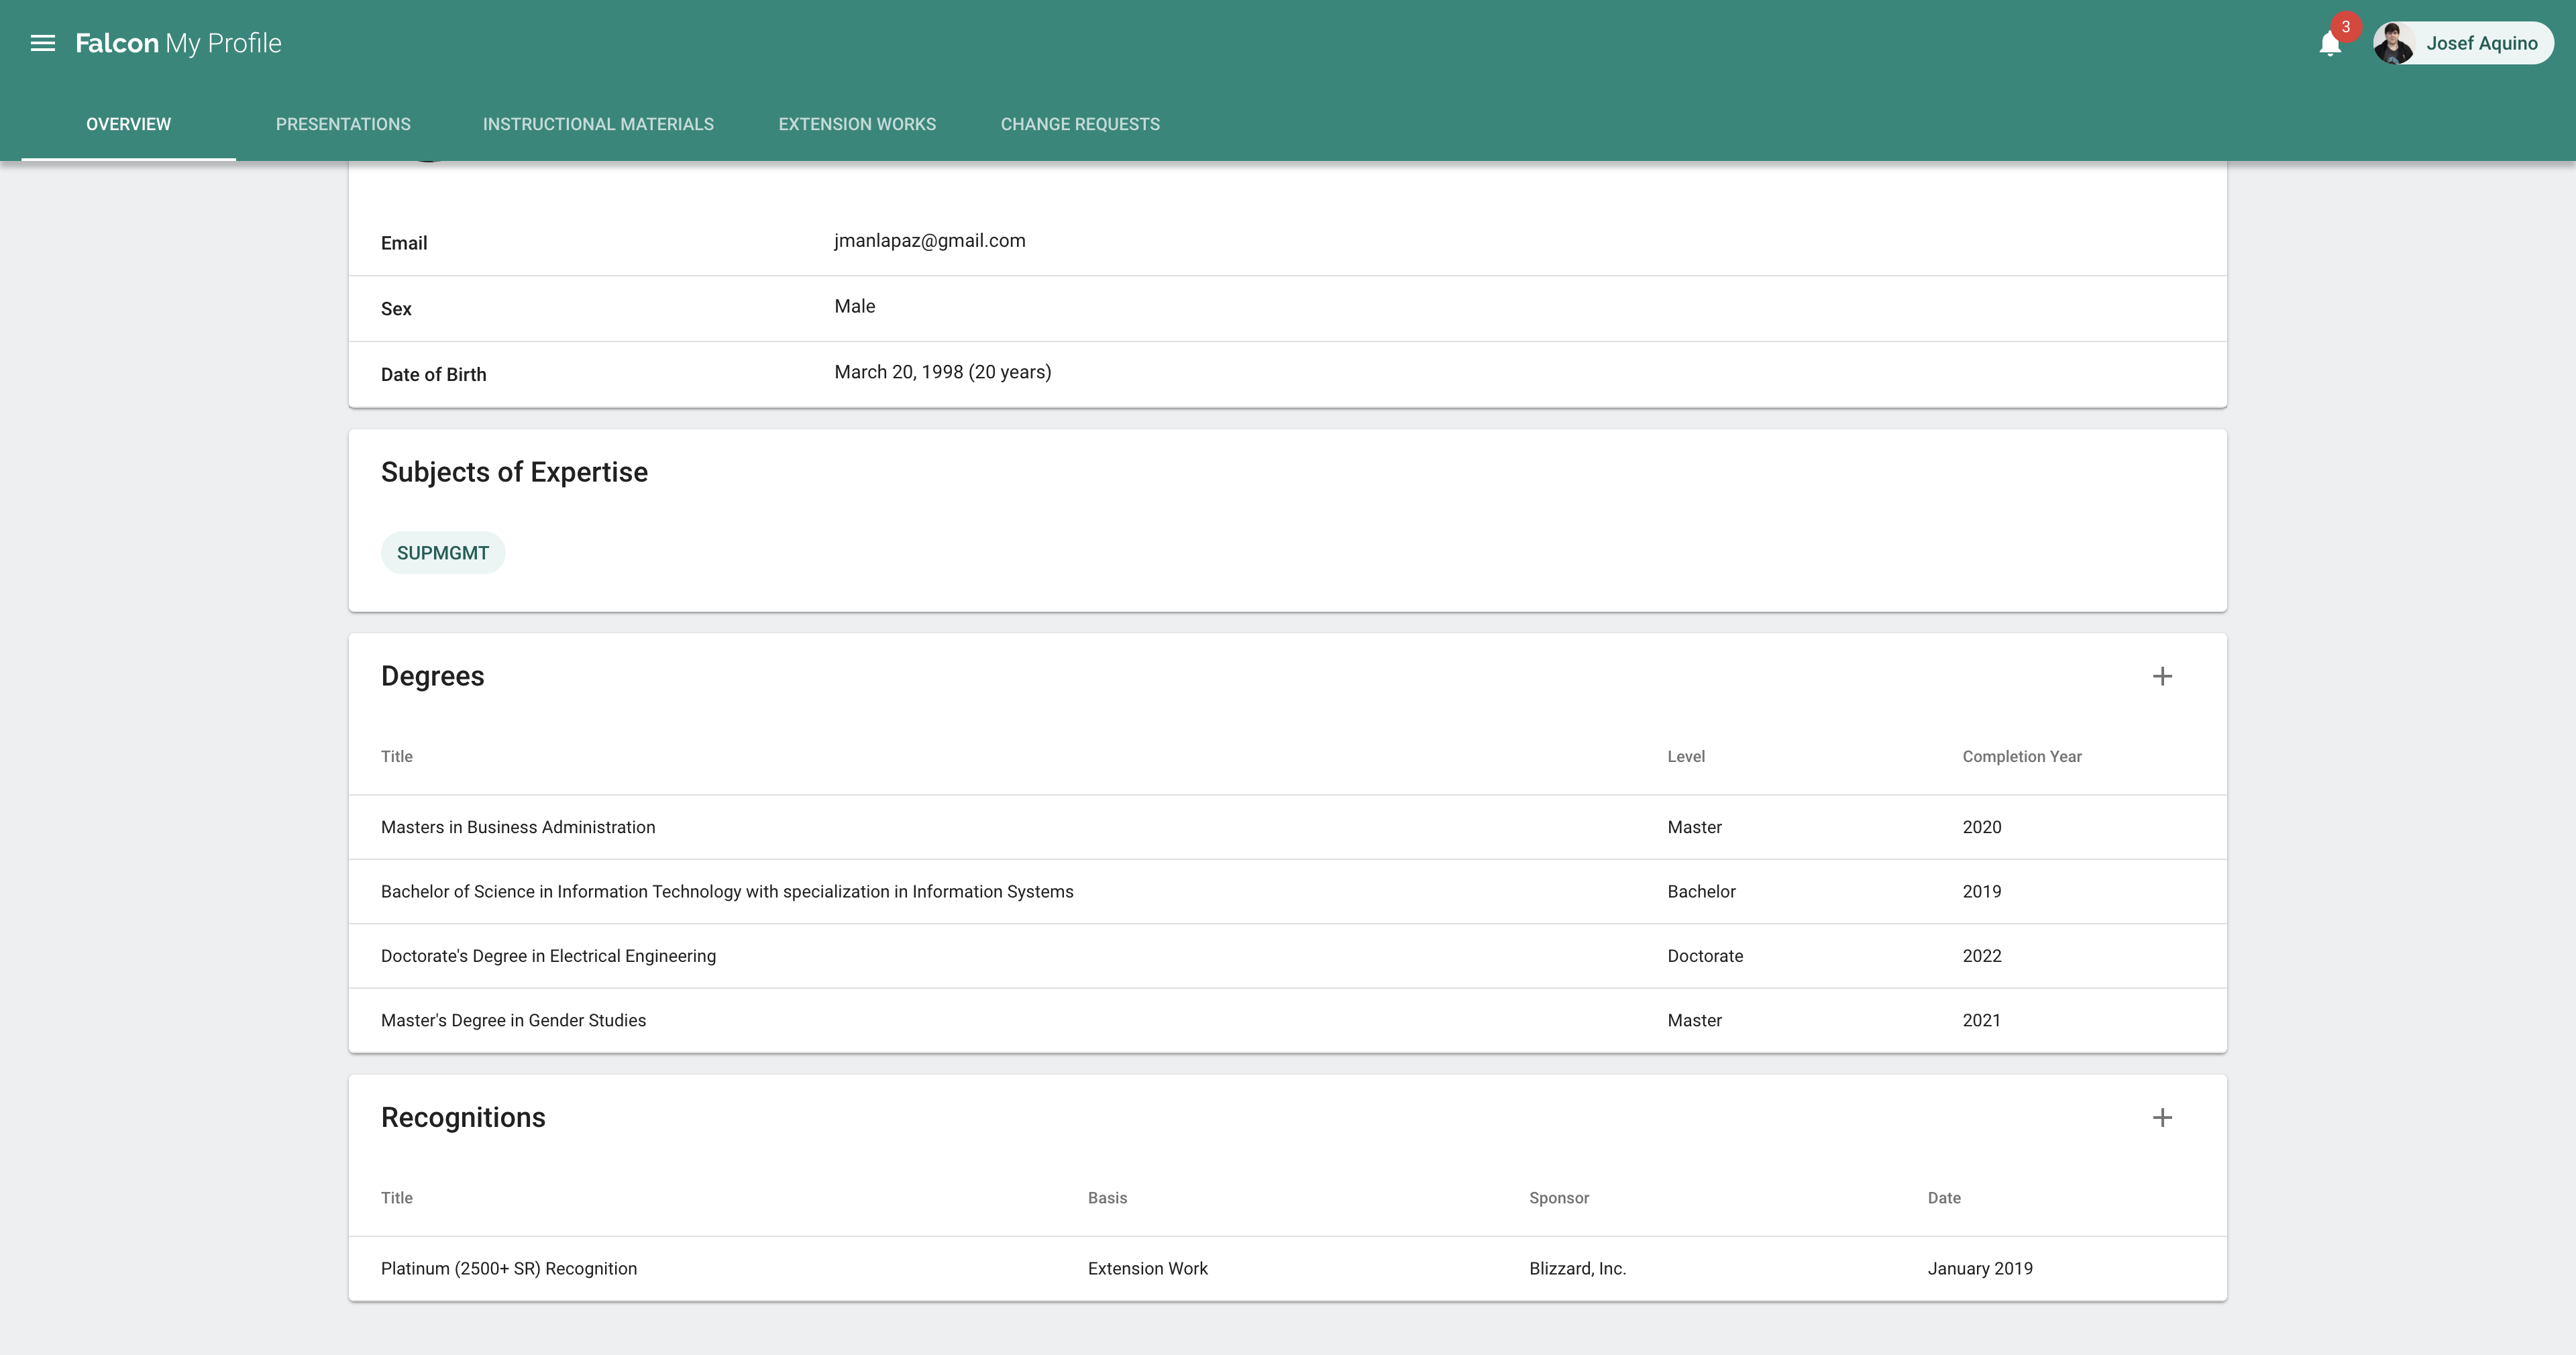
\includegraphics[width=\linewidth]{figures/screen_specifications/myprofile_screens/my_profileB.png}
   \caption{My Profile Overview Screen B}
   }
   
   \pagebreak
   
   \subsubsection{My Profile Presentation}
    
    \field{Screen Name}{My Profile Presentation}
    
    \field{File Name}{/pages/FacultyProfiles/components/faculty_detail_tabs/PresentationsTab/index.js}
    
    \field{Description} {Displays the list of presentations}
    
  of the profile. It also shows the details of each presentation, such as the category, date, sponsor, venue, conference, medium, and duration. faculty   \field{Layout}{}
    
\makefigure{!h}{
   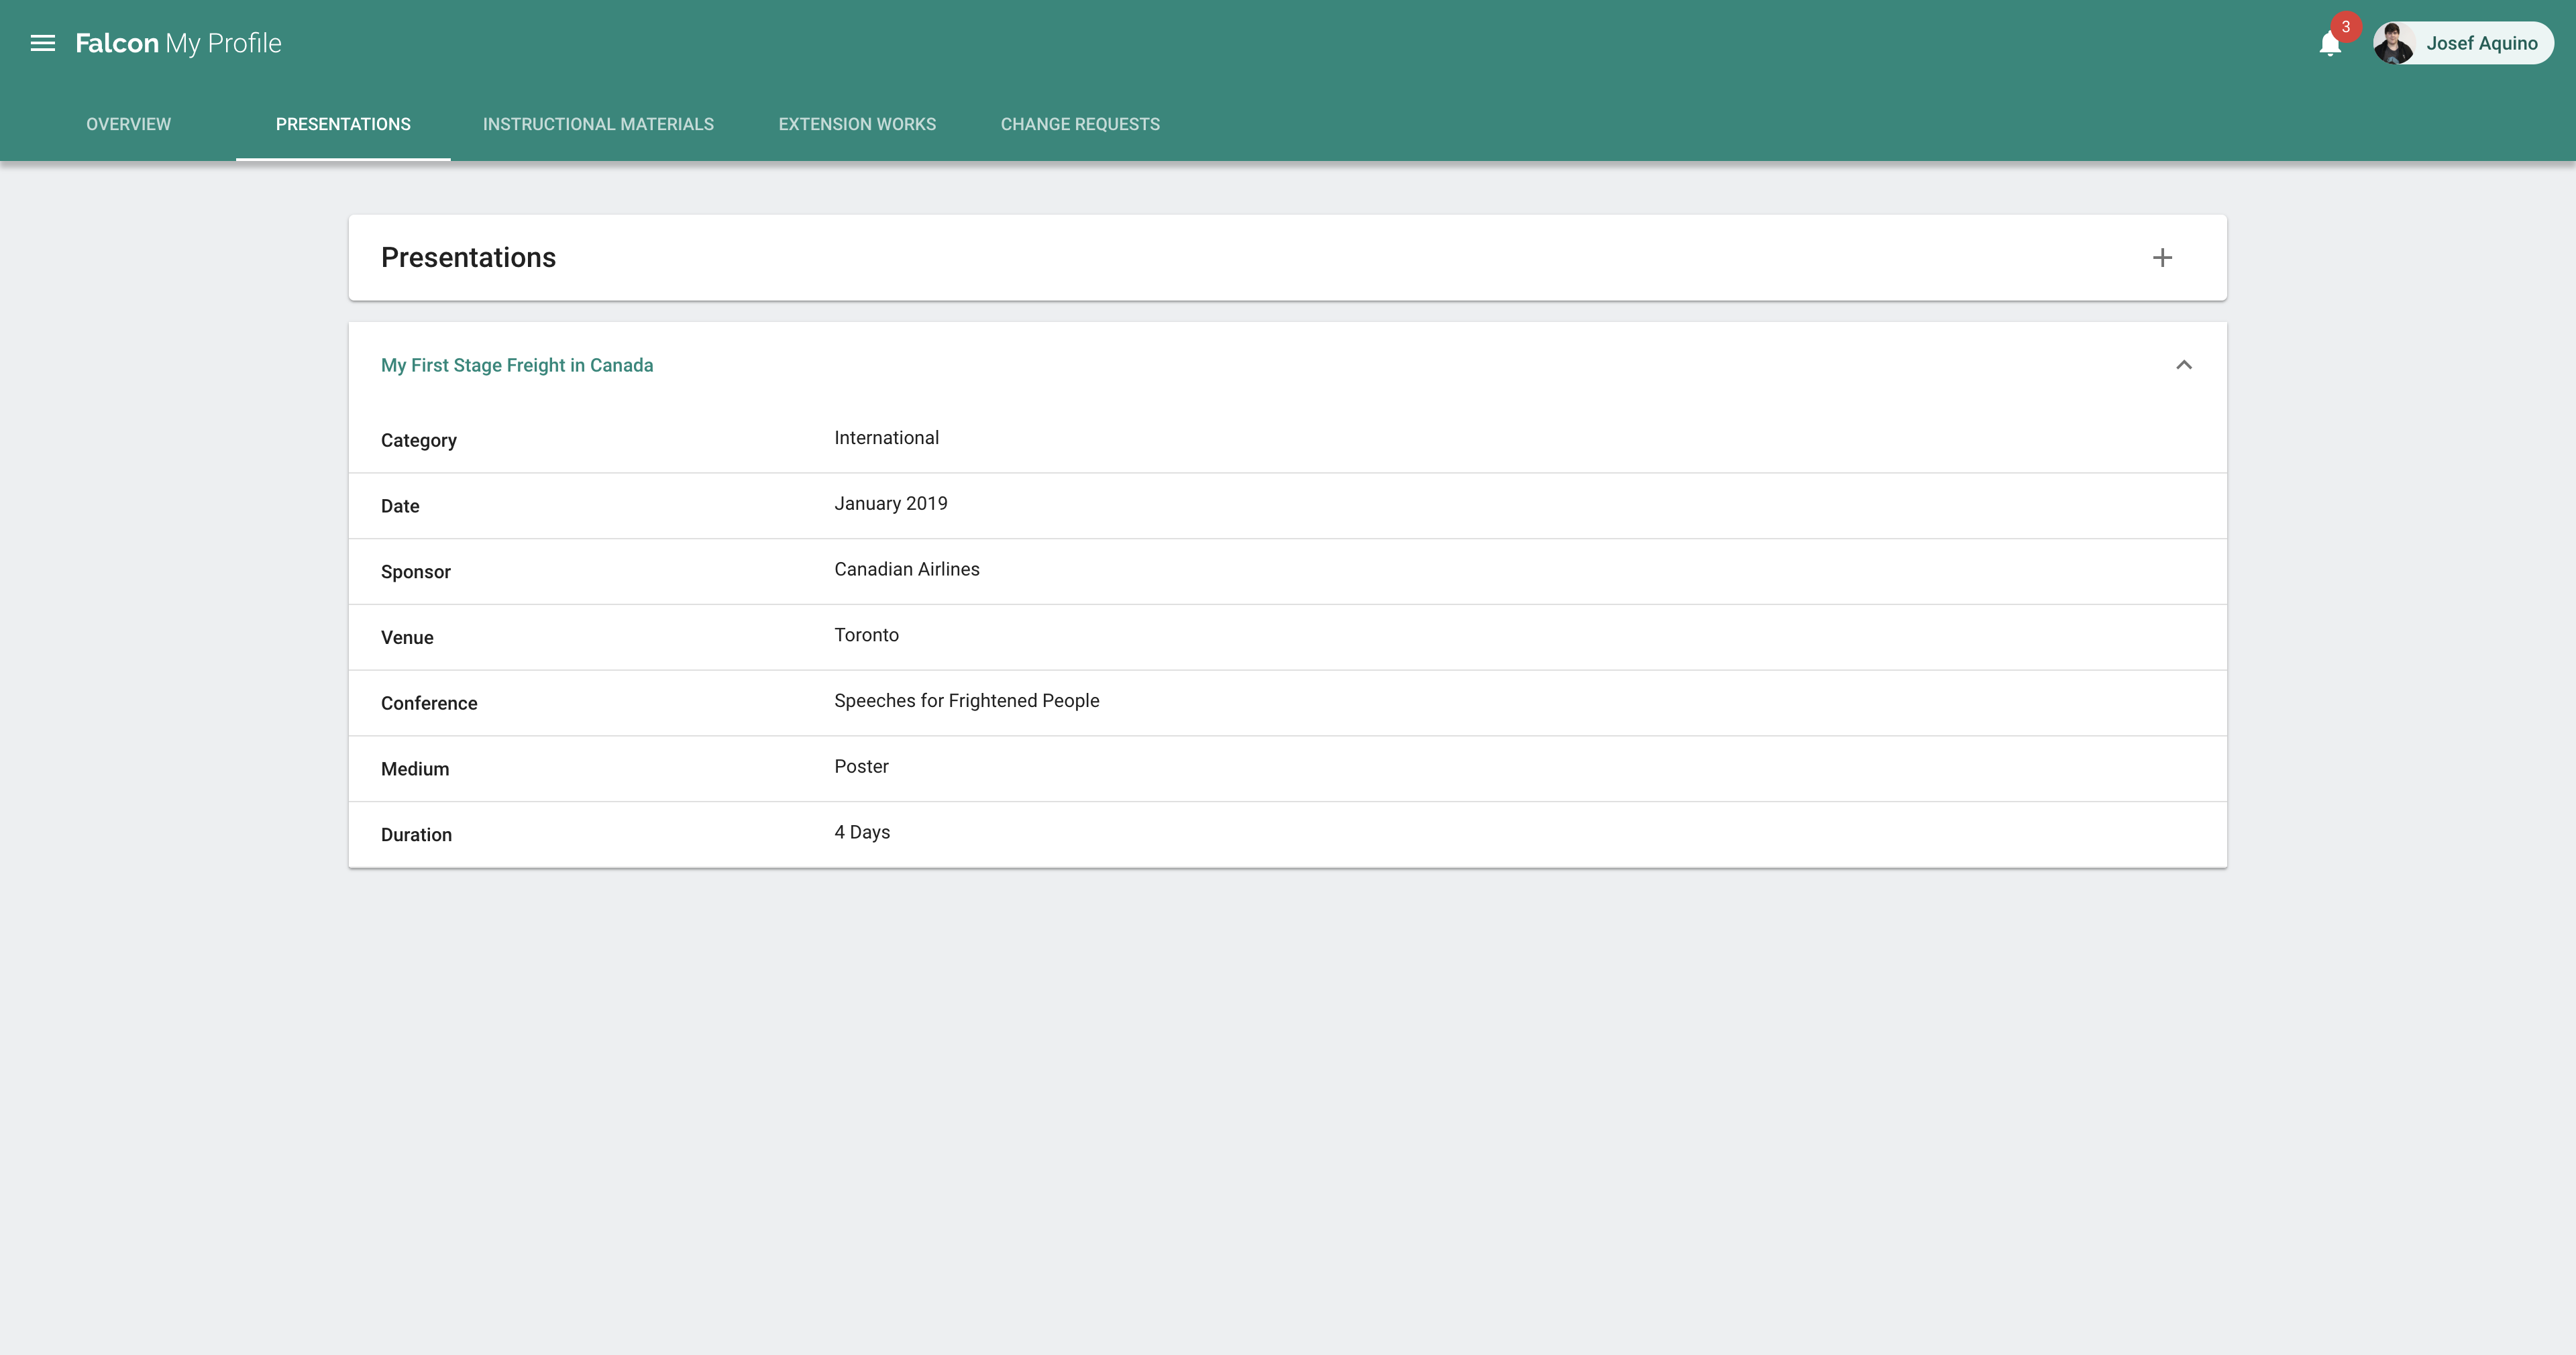
\includegraphics[width=\linewidth]{figures/screen_specifications/myprofile_screens/myprofile_presentation.png}
   \caption{My Profile Presentation Screen A}
   }

    \pagebreak
    
    \subsubsection{My Profile Instructional Materials}
    
    \field{Screen Name}{My Profile Instructional Materials}
    
    \field{File Name}{/pages/FacultyProfiles/components/faculty_detail_tabs/InstructionalMaterialsTab/index.js}
    
    \field{Description} {Displays the list of instructional materials of the faculty profile. It also shows the details of each instructional material, such as the category, date, sponsor, venue, conference, medium, and duration.}
    
    \field{Layout}{}
    
\makefigure{!h}{
   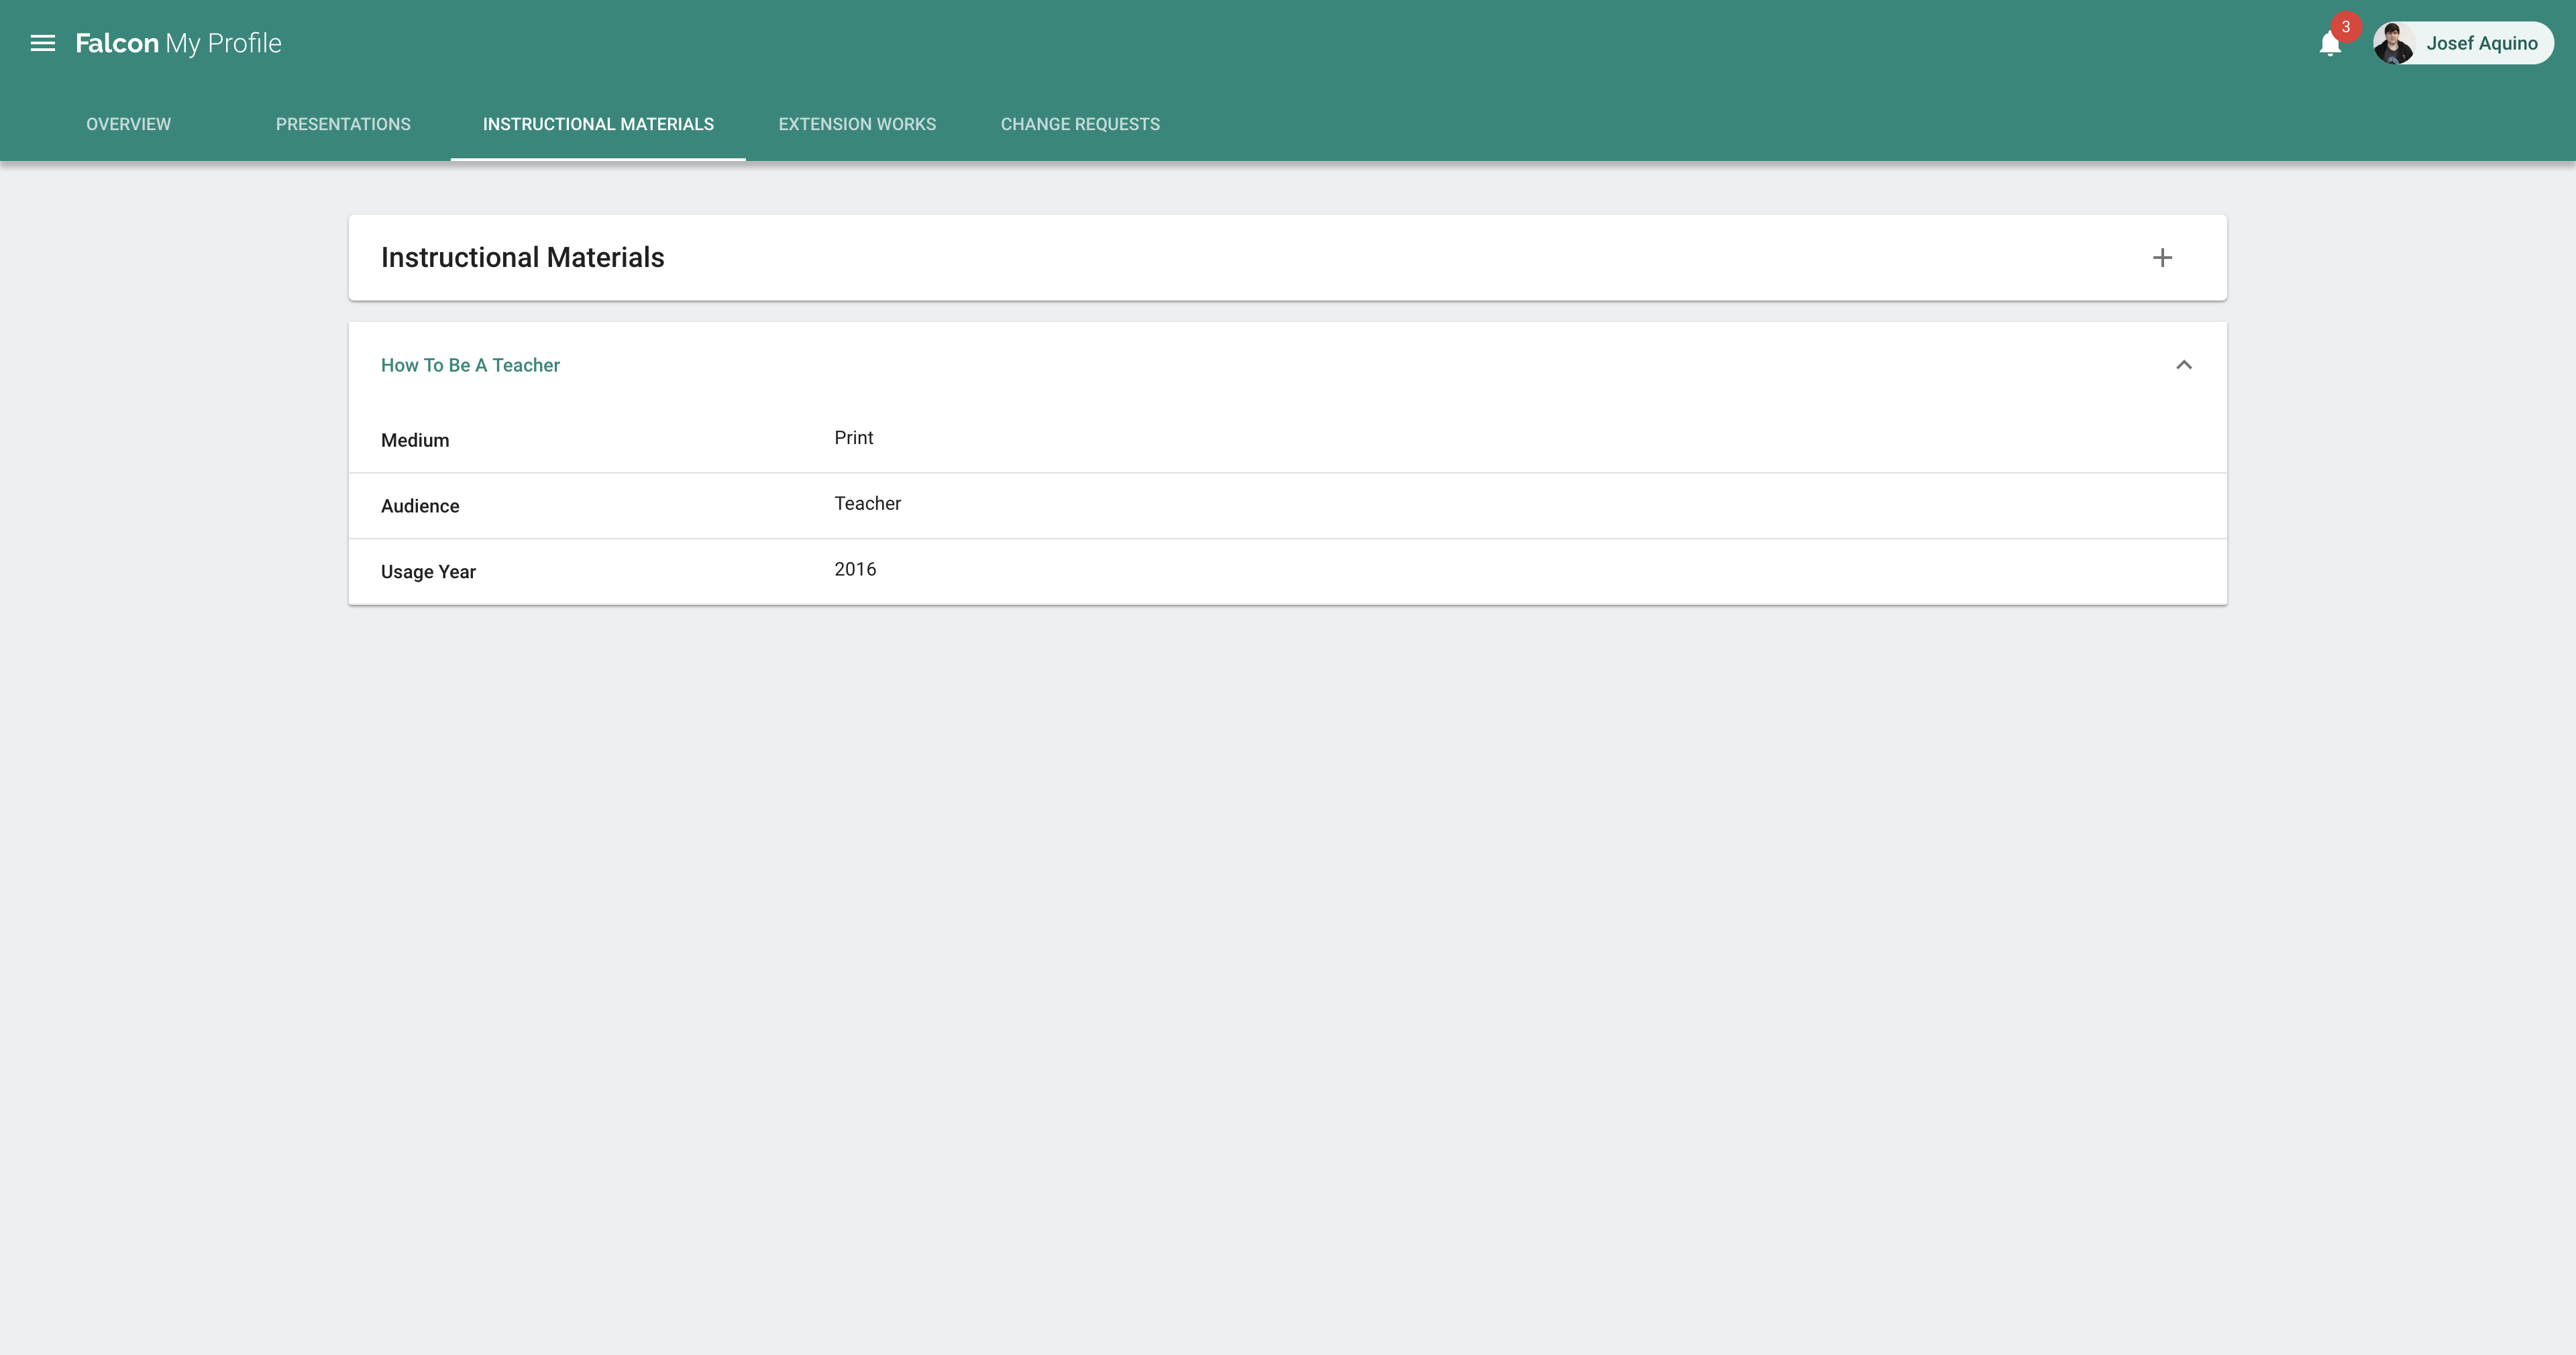
\includegraphics[width=\linewidth]{figures/screen_specifications/myprofile_screens/myprofile_instructional.png}
   \caption{My Profile Presentation Screen}
   }

    \pagebreak
    
    \subsubsection{My Profile Extension Works}
    
    \field{Screen Name}{My Profile Extension Works}
    
    \field{File Name}{/pages/FacultyProfiles/components/faculty_detail_tabs/ExtensionWorksTab/index.js}
    
    \field{Description} {Displays the list of extension works of the faculty profile. It also shows the details of each extension work, such as the venue and role.}
    
    \field{Layout}{}
    
\makefigure{!h}{
   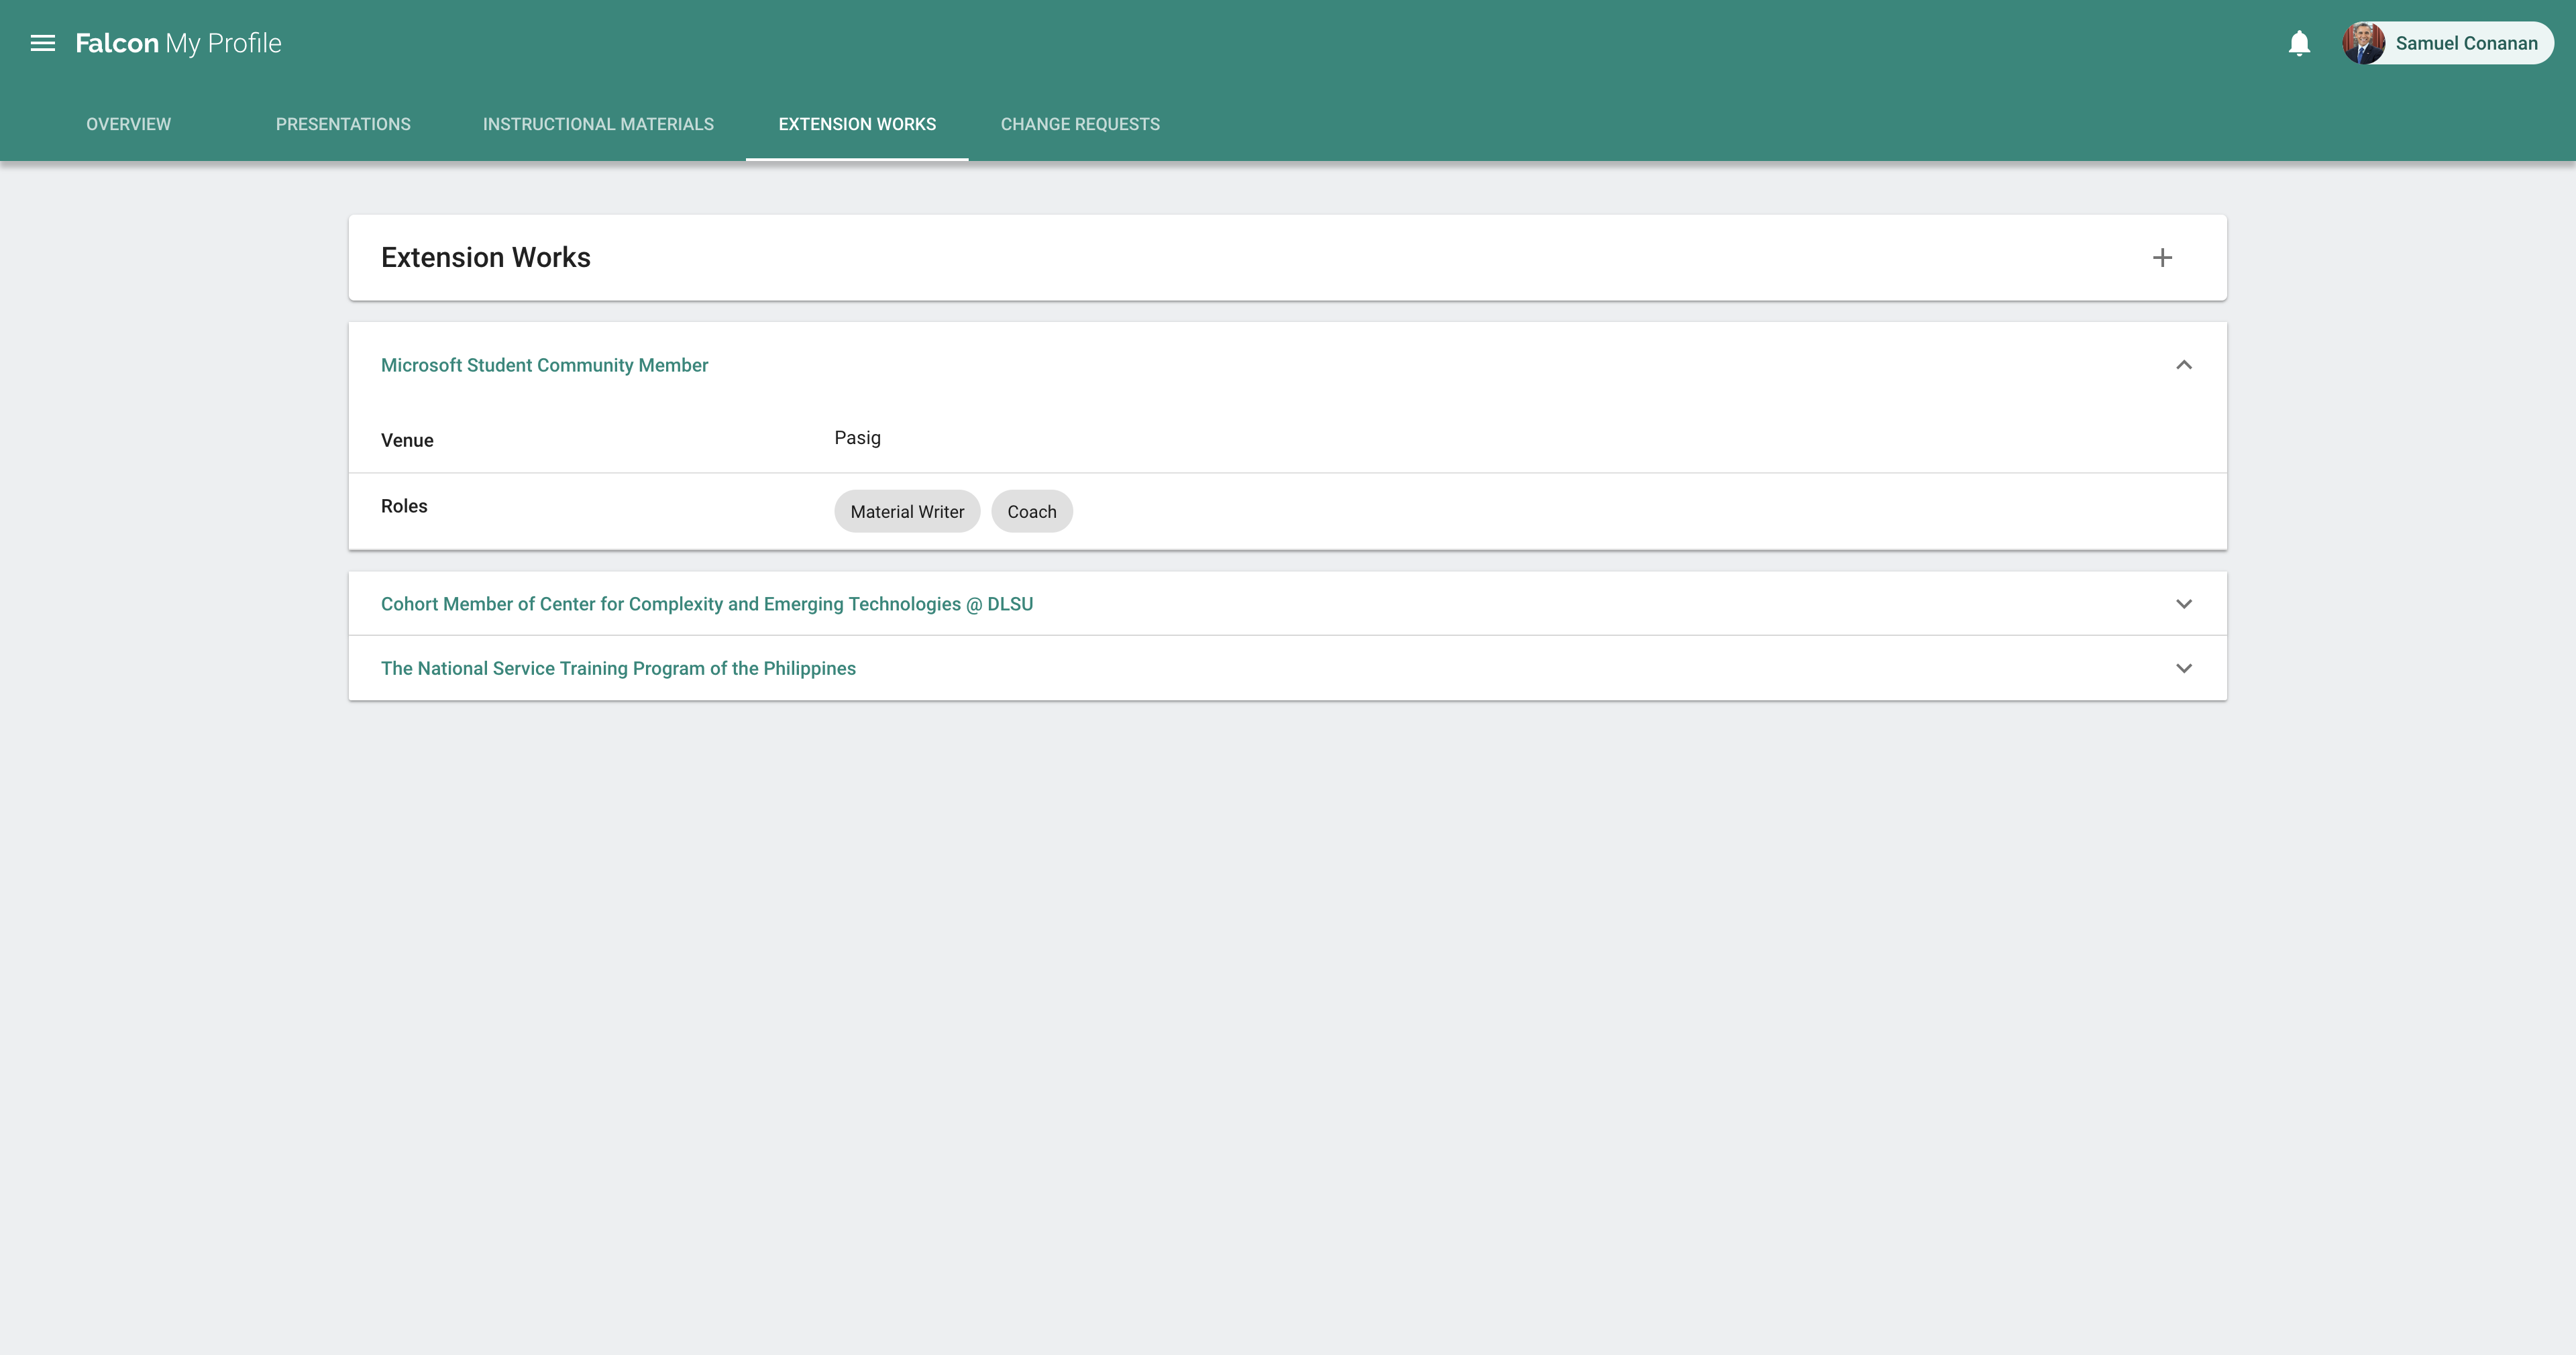
\includegraphics[width=\linewidth]{figures/screen_specifications/myprofile_screens/myprofile_extension.png}
   \caption{My Profile Extension Works Screen}
   }

    \pagebreak
    
    \subsubsection{My Profile Change Requests}
    
    \field{Screen Name}{My Profile Change Requests}
    
    \field{File Name}{/pages/FacultyProfiles/components/faculty_detail_tabs/ChangeRequestsTab/index.js}
    
    \field{Description} {Displays the list of change requests of the faculty profile. It also shows the details of each change request and status.}
    
    \field{Layout}{}
    
\makefigure{!h}{
   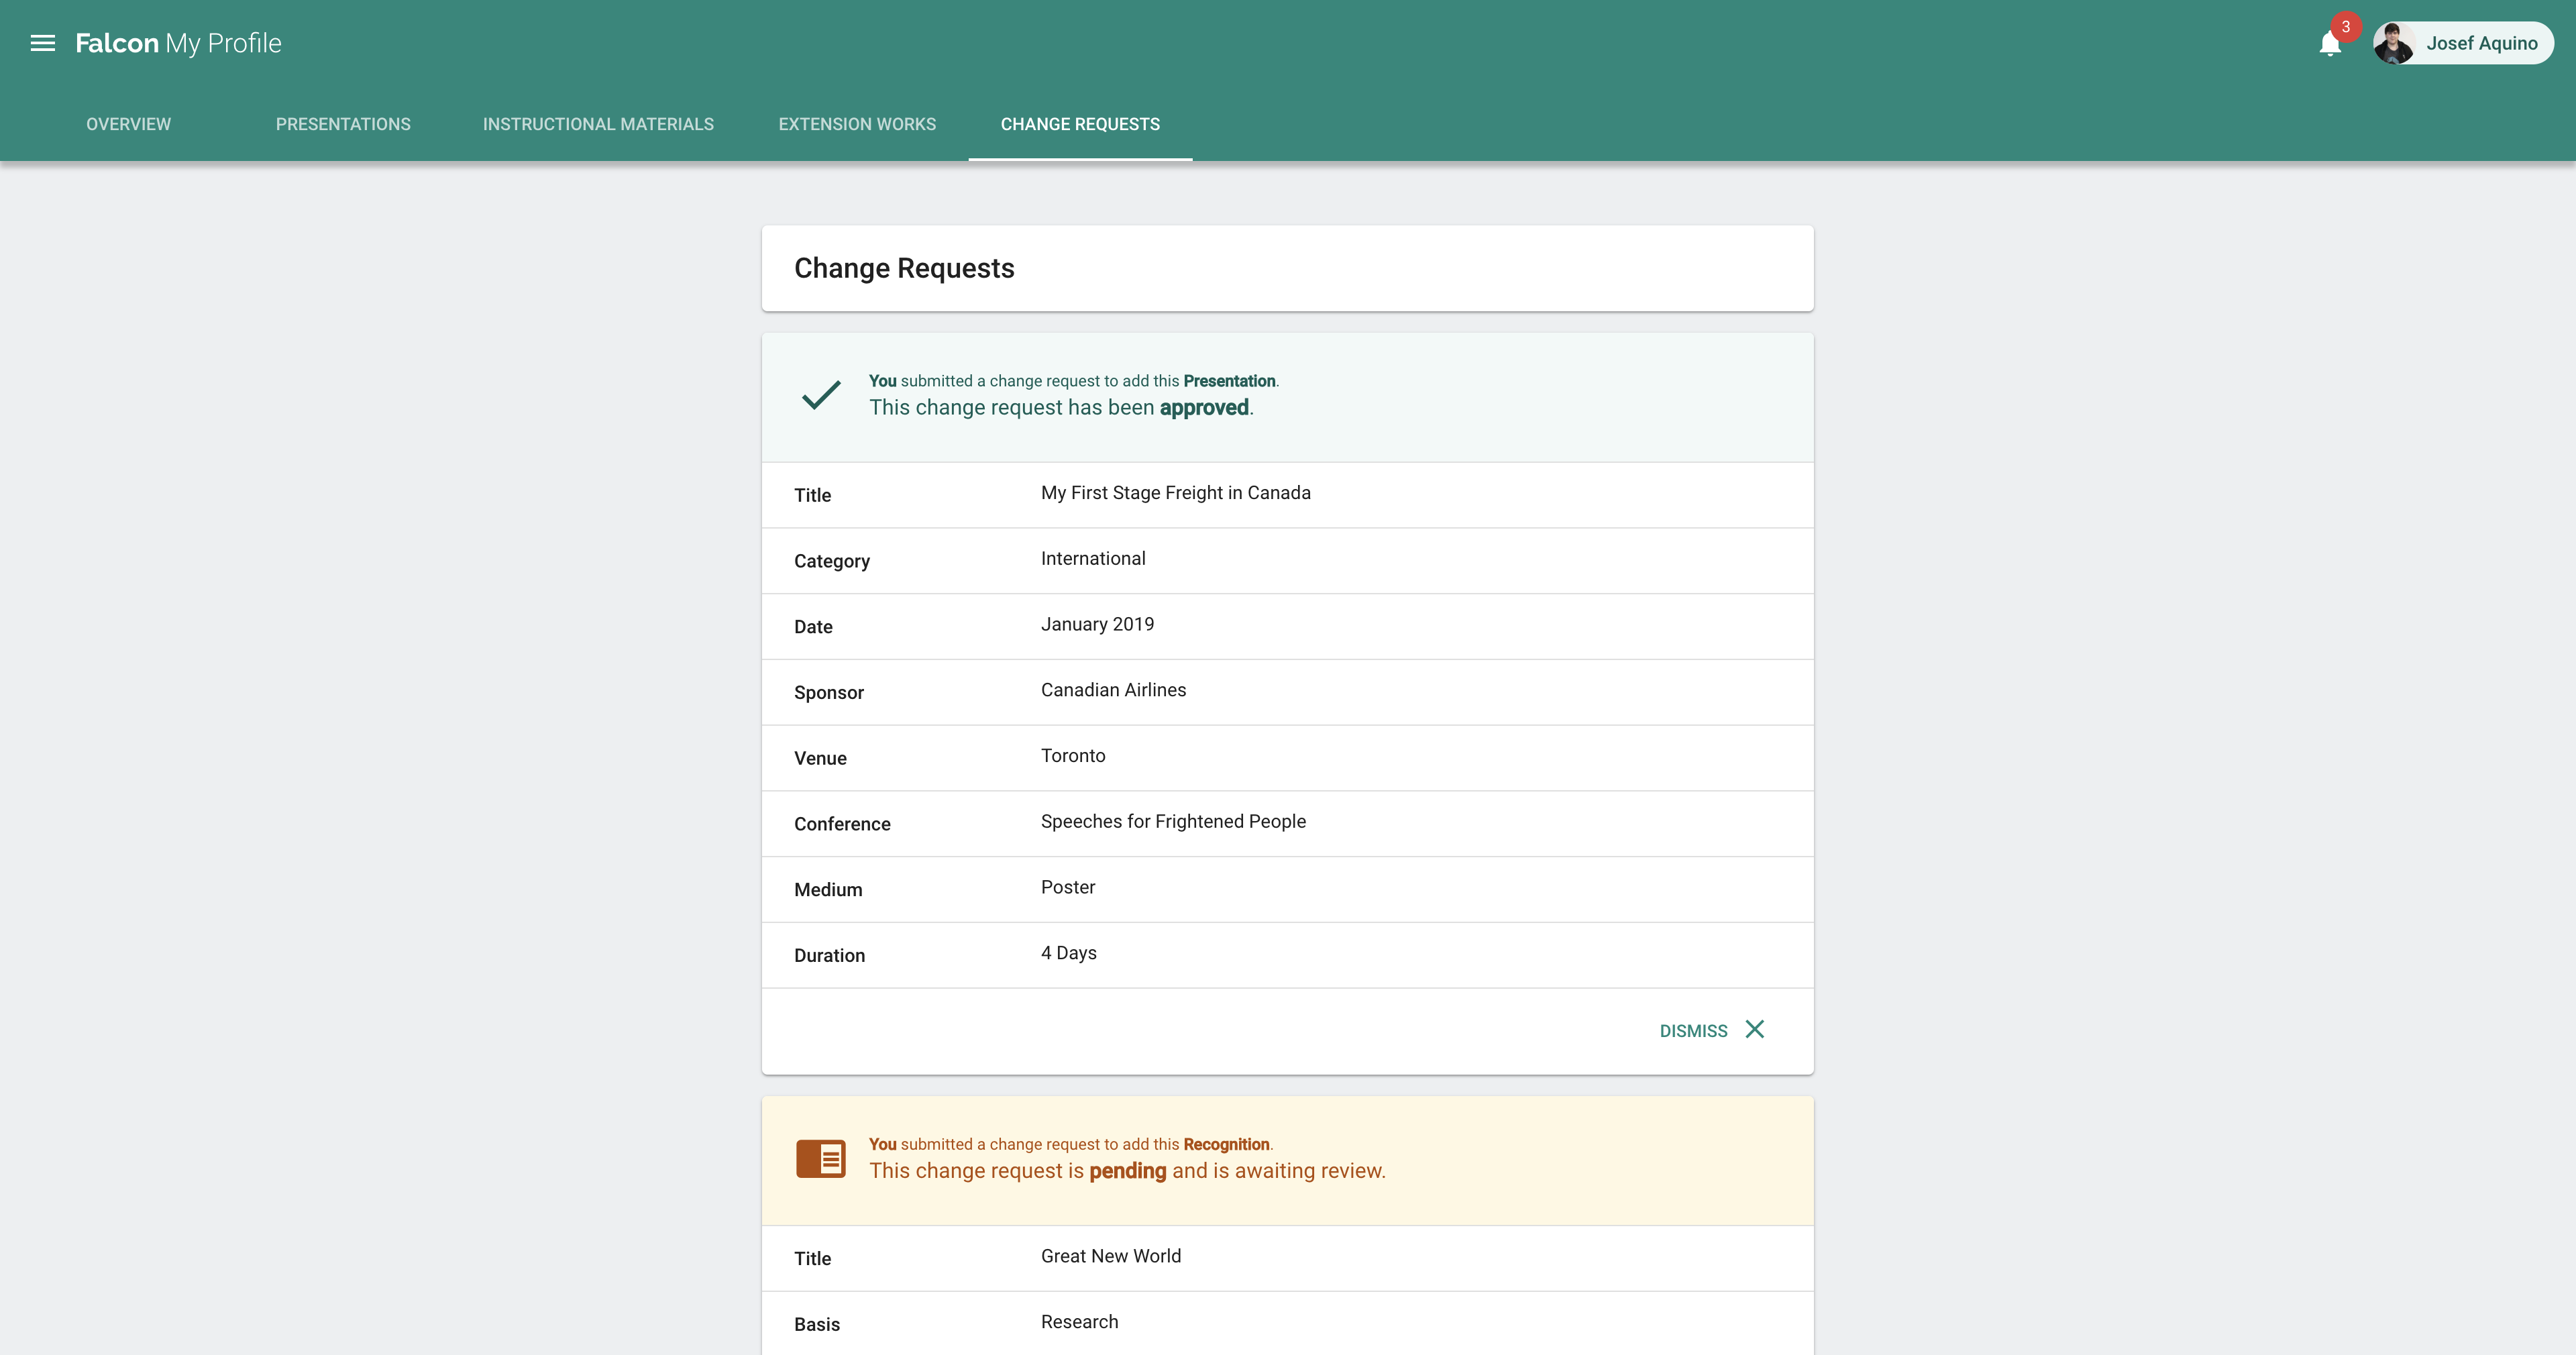
\includegraphics[width=\linewidth]{figures/screen_specifications/myprofile_screens/myprofile_changeA.png}
   \caption{My Profile Change Request A}
   }
   
\makefigure{!h}{
   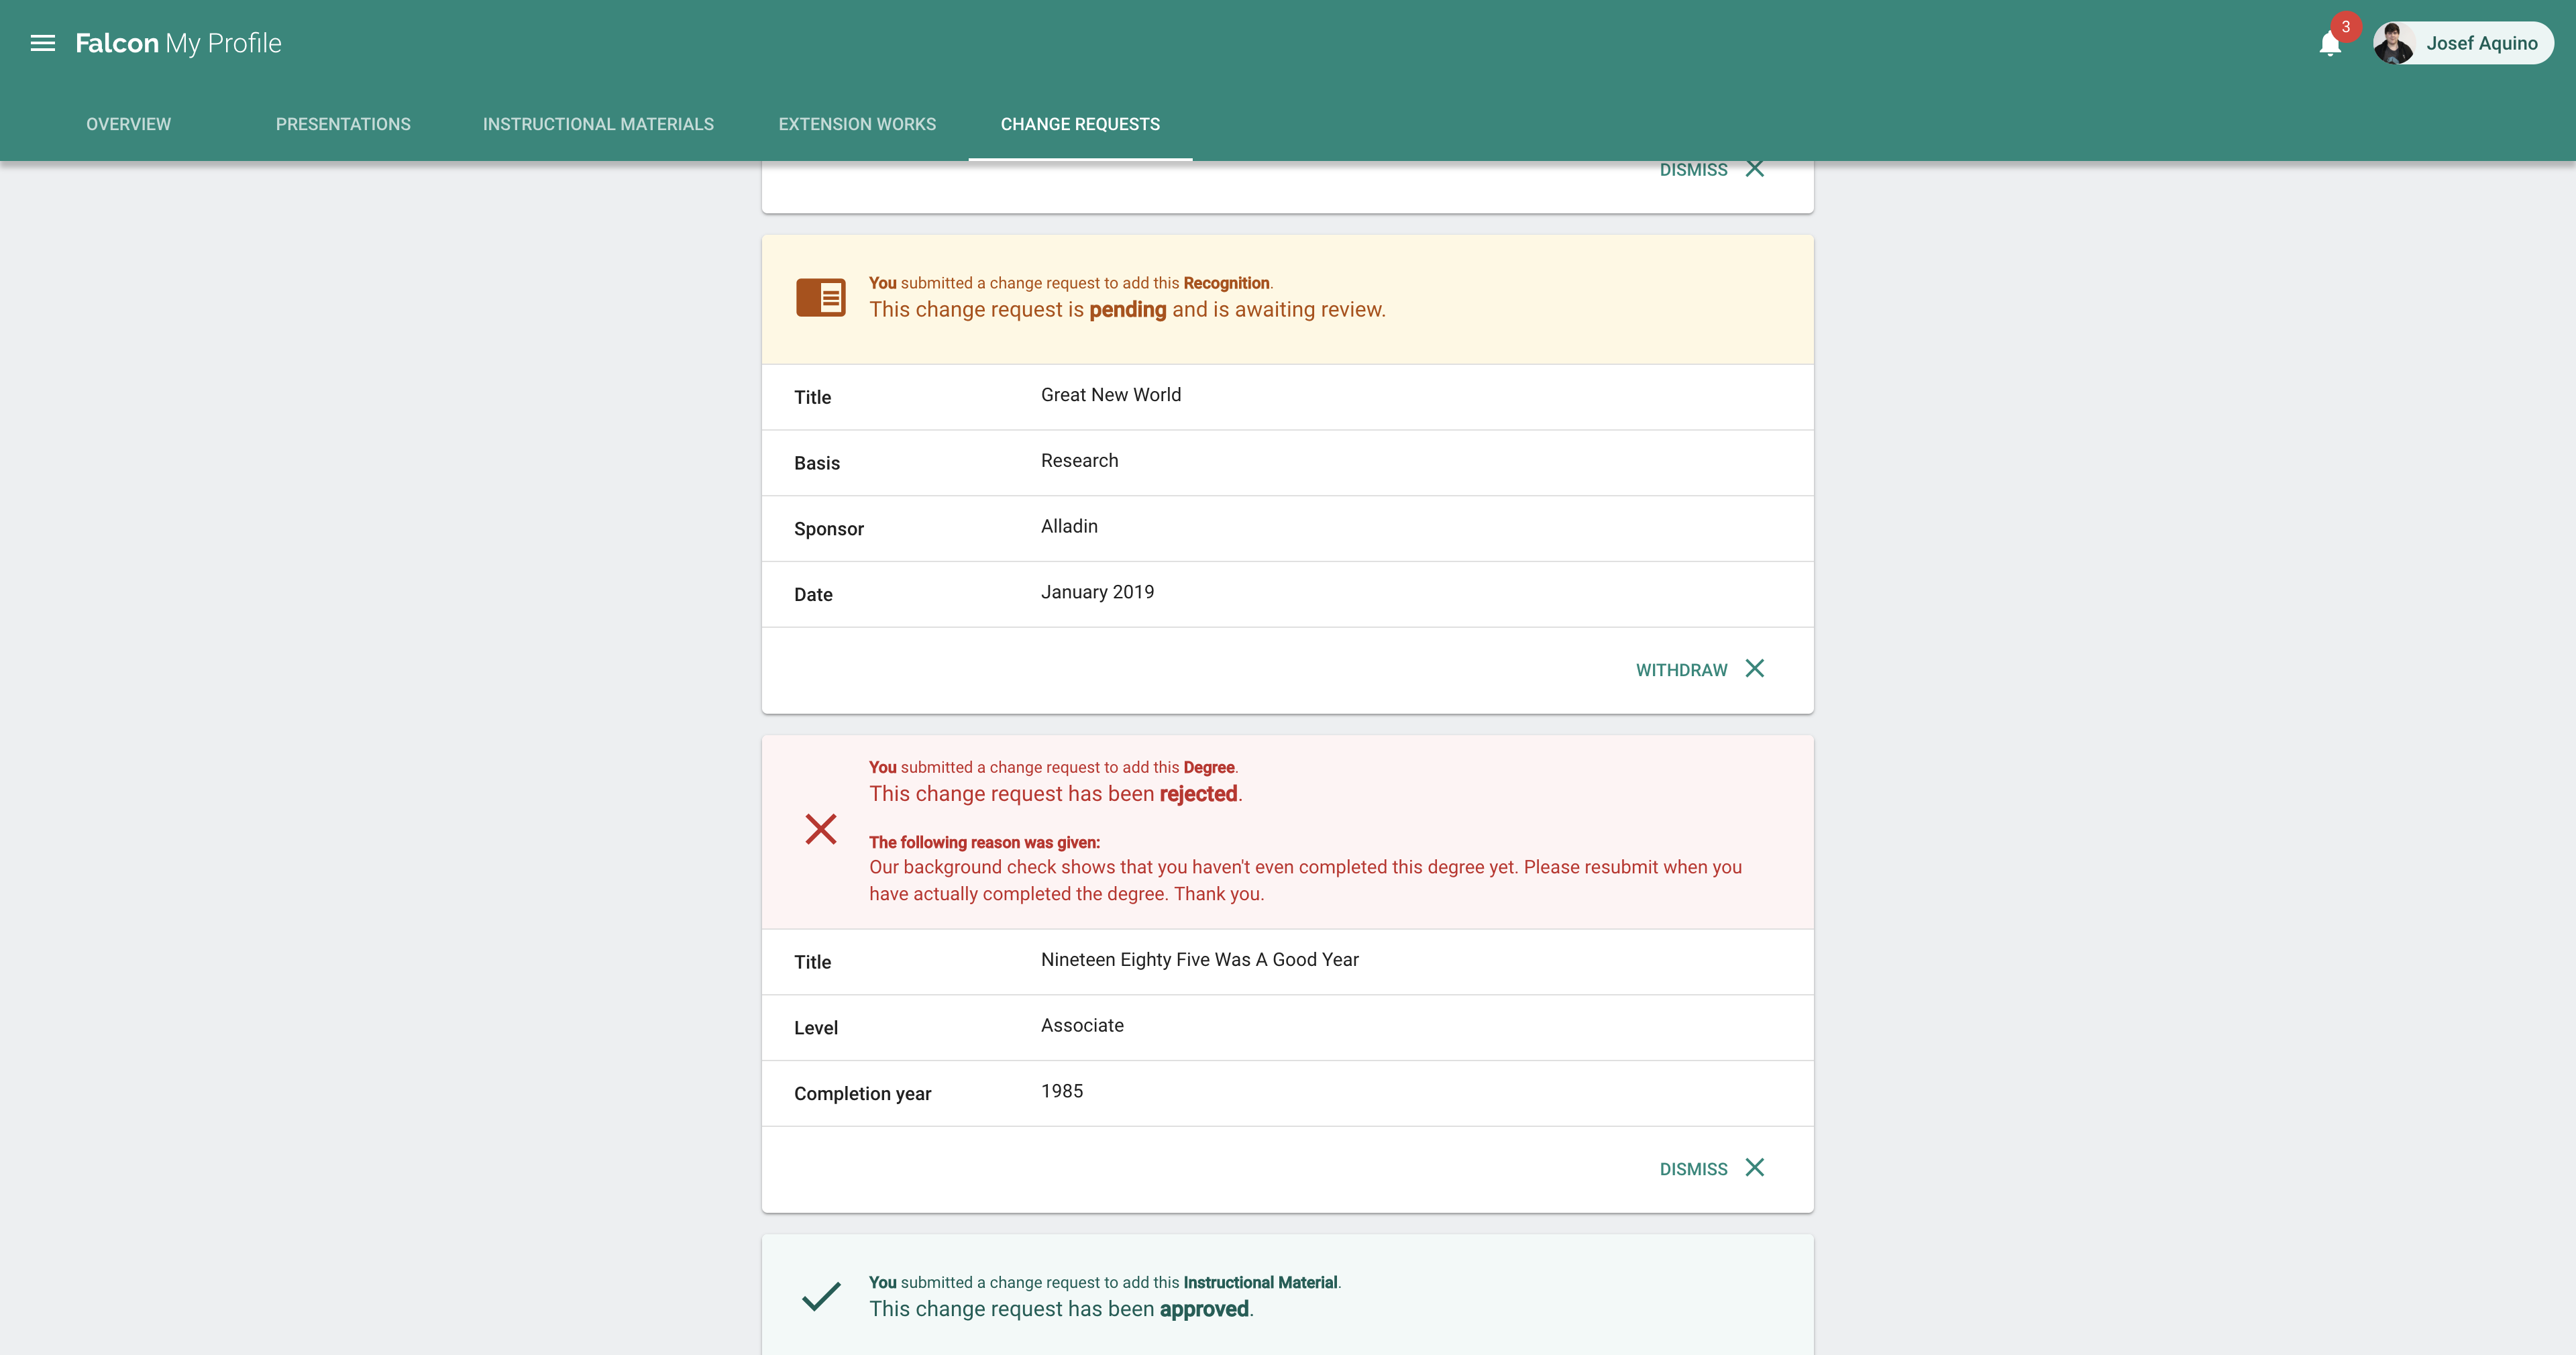
\includegraphics[width=\linewidth]{figures/screen_specifications/myprofile_screens/myprofile_changeB.png}
   \caption{My Profile Change Request B}
   }

    \pagebreak
    
    \subsubsection{My Profile Password Notification}
    
    \field{Screen Name}{My Profile Password Notification}
    
    \field{File Name}{/pages/SignIn/components/PasswordSetupCard/index.js}
    
    \field{Description} {Notifies the faculty member that the password for their faculty profile has been reset and they are currently using a temporary password. This also reminds faculty members that they must manually change their password.}
    
    \field{Layout}{}
    
\makefigure{!h}{
   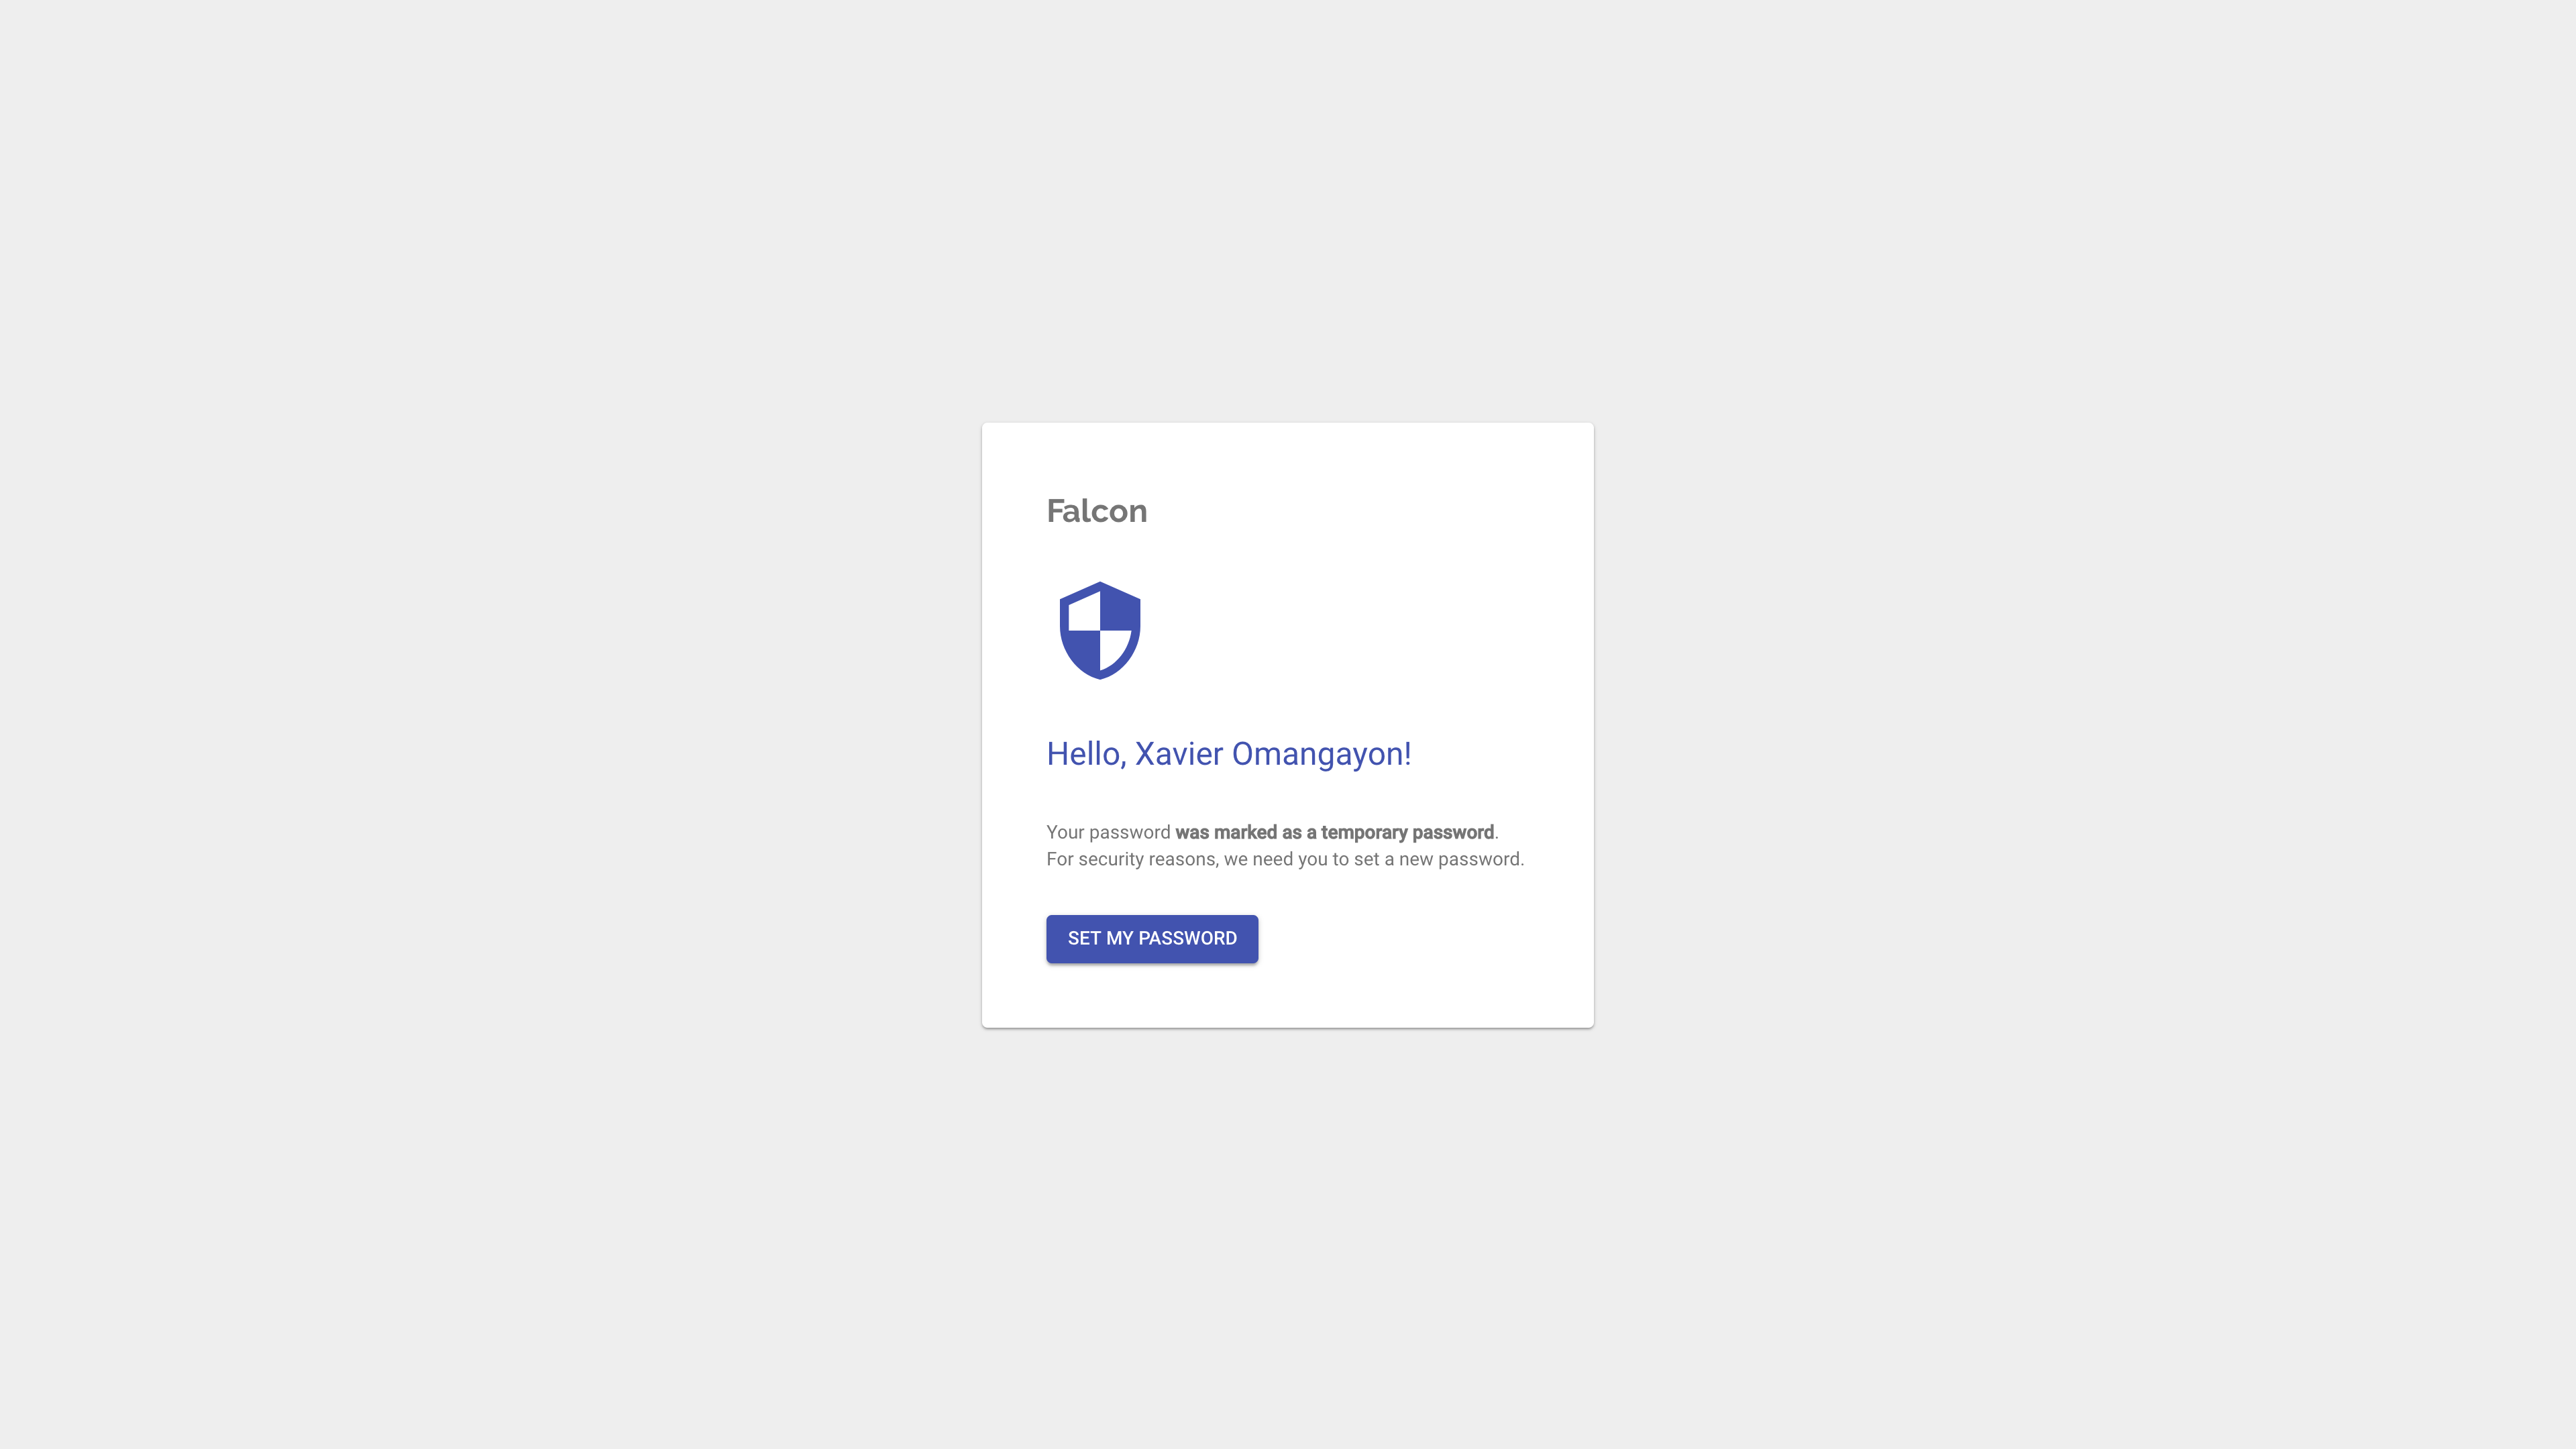
\includegraphics[width=\linewidth]{figures/screen_specifications/myprofile_screens/password_notification.png}
   \caption{My Profile Password Notification Screen}
   }

    \pagebreak
    
    
    \subsection{Faculty Loading}
    
    \subsubsection{Faculty Loading Screen}
    
    \field{Screen Name}{Faculty Loading}
    
    \field{File Name}{/pages/FacultyLoading/index.js}
    
    \field{Description} {Displays the schedule with list of classes. The clerk may switch between terms and days to set the schedule. The left of the screen also displays the list of faculty members, which the clerk may drag-and-drop to their respective classes.}
    
    \field{Layout}{}
    
\makefigure{!h}{
   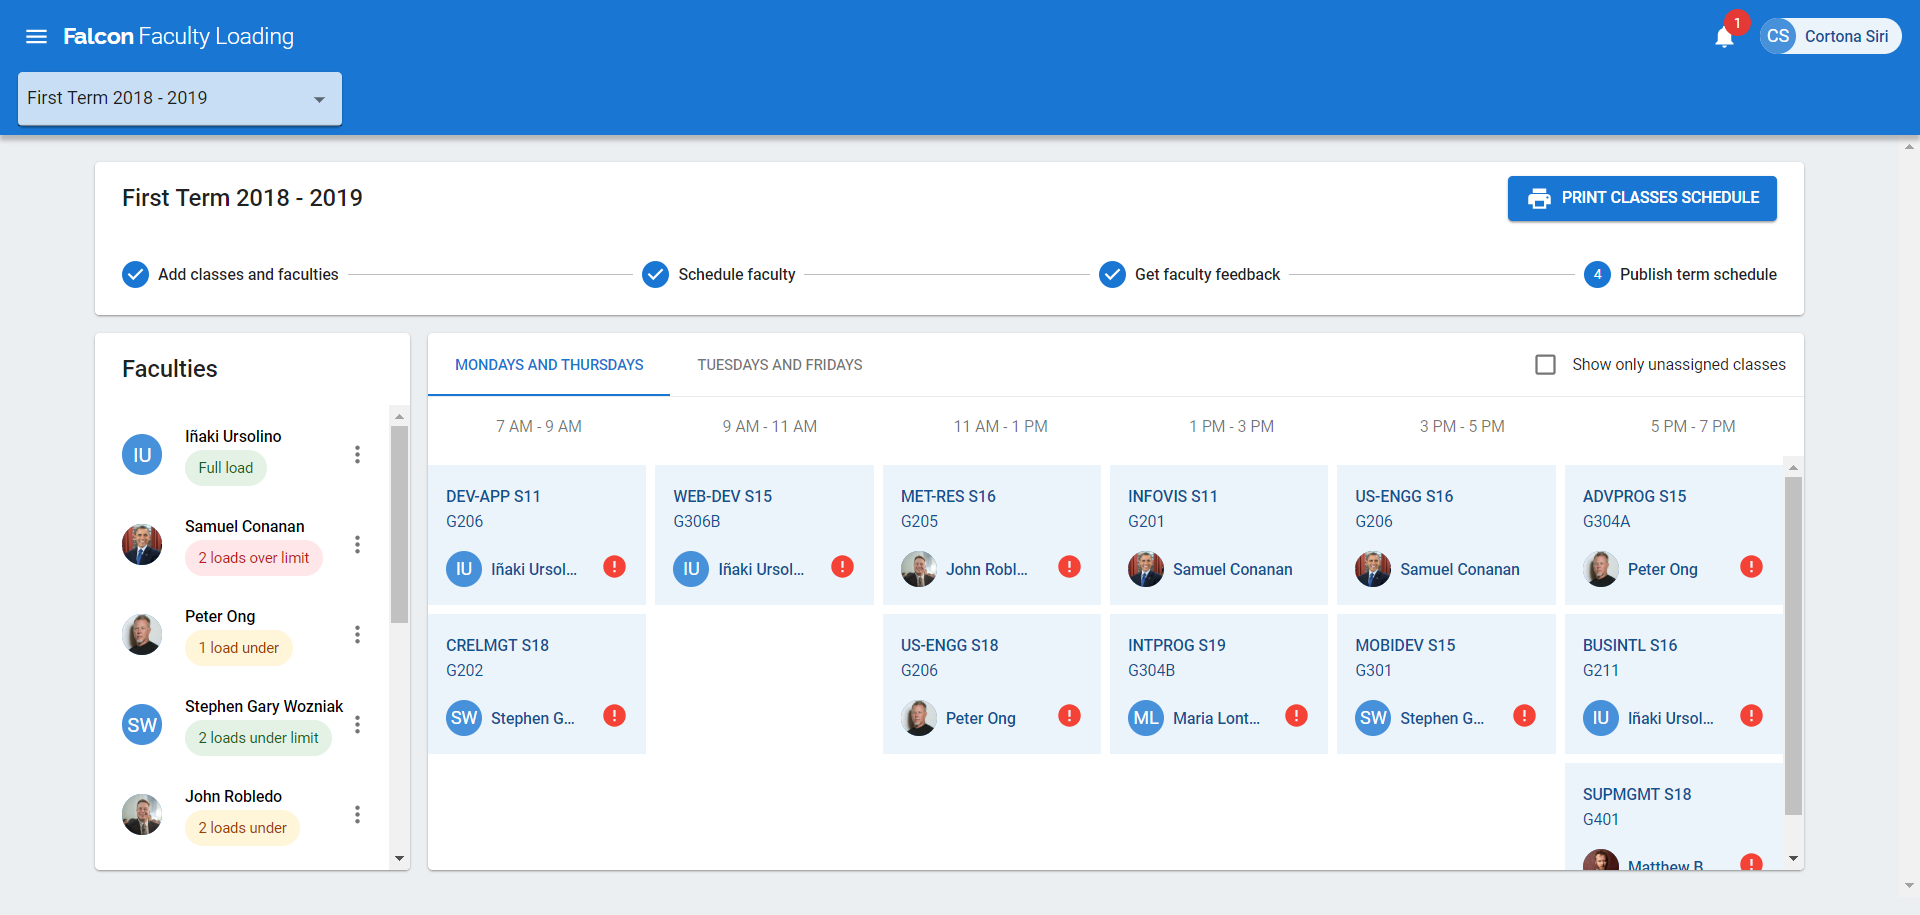
\includegraphics[width=\linewidth]{figures/screen_specifications/faculty_loading_screens/faculty_loading.png}
   \caption{Faculty Loading Screen}
   }
   
   \pagebreak
   
   \subsubsection{Time Availability}
    
    \field{Screen Name}{Time Availability}
    
    \field{File Name}{/pages/FacultyLoading/components/modals/FacultyAvailabilityModal/index.js}
    
    \field{Description} {Displays the days and times of the faculty members.}
    
    \field{Layout}{}
    
\makefigure{!h}{
   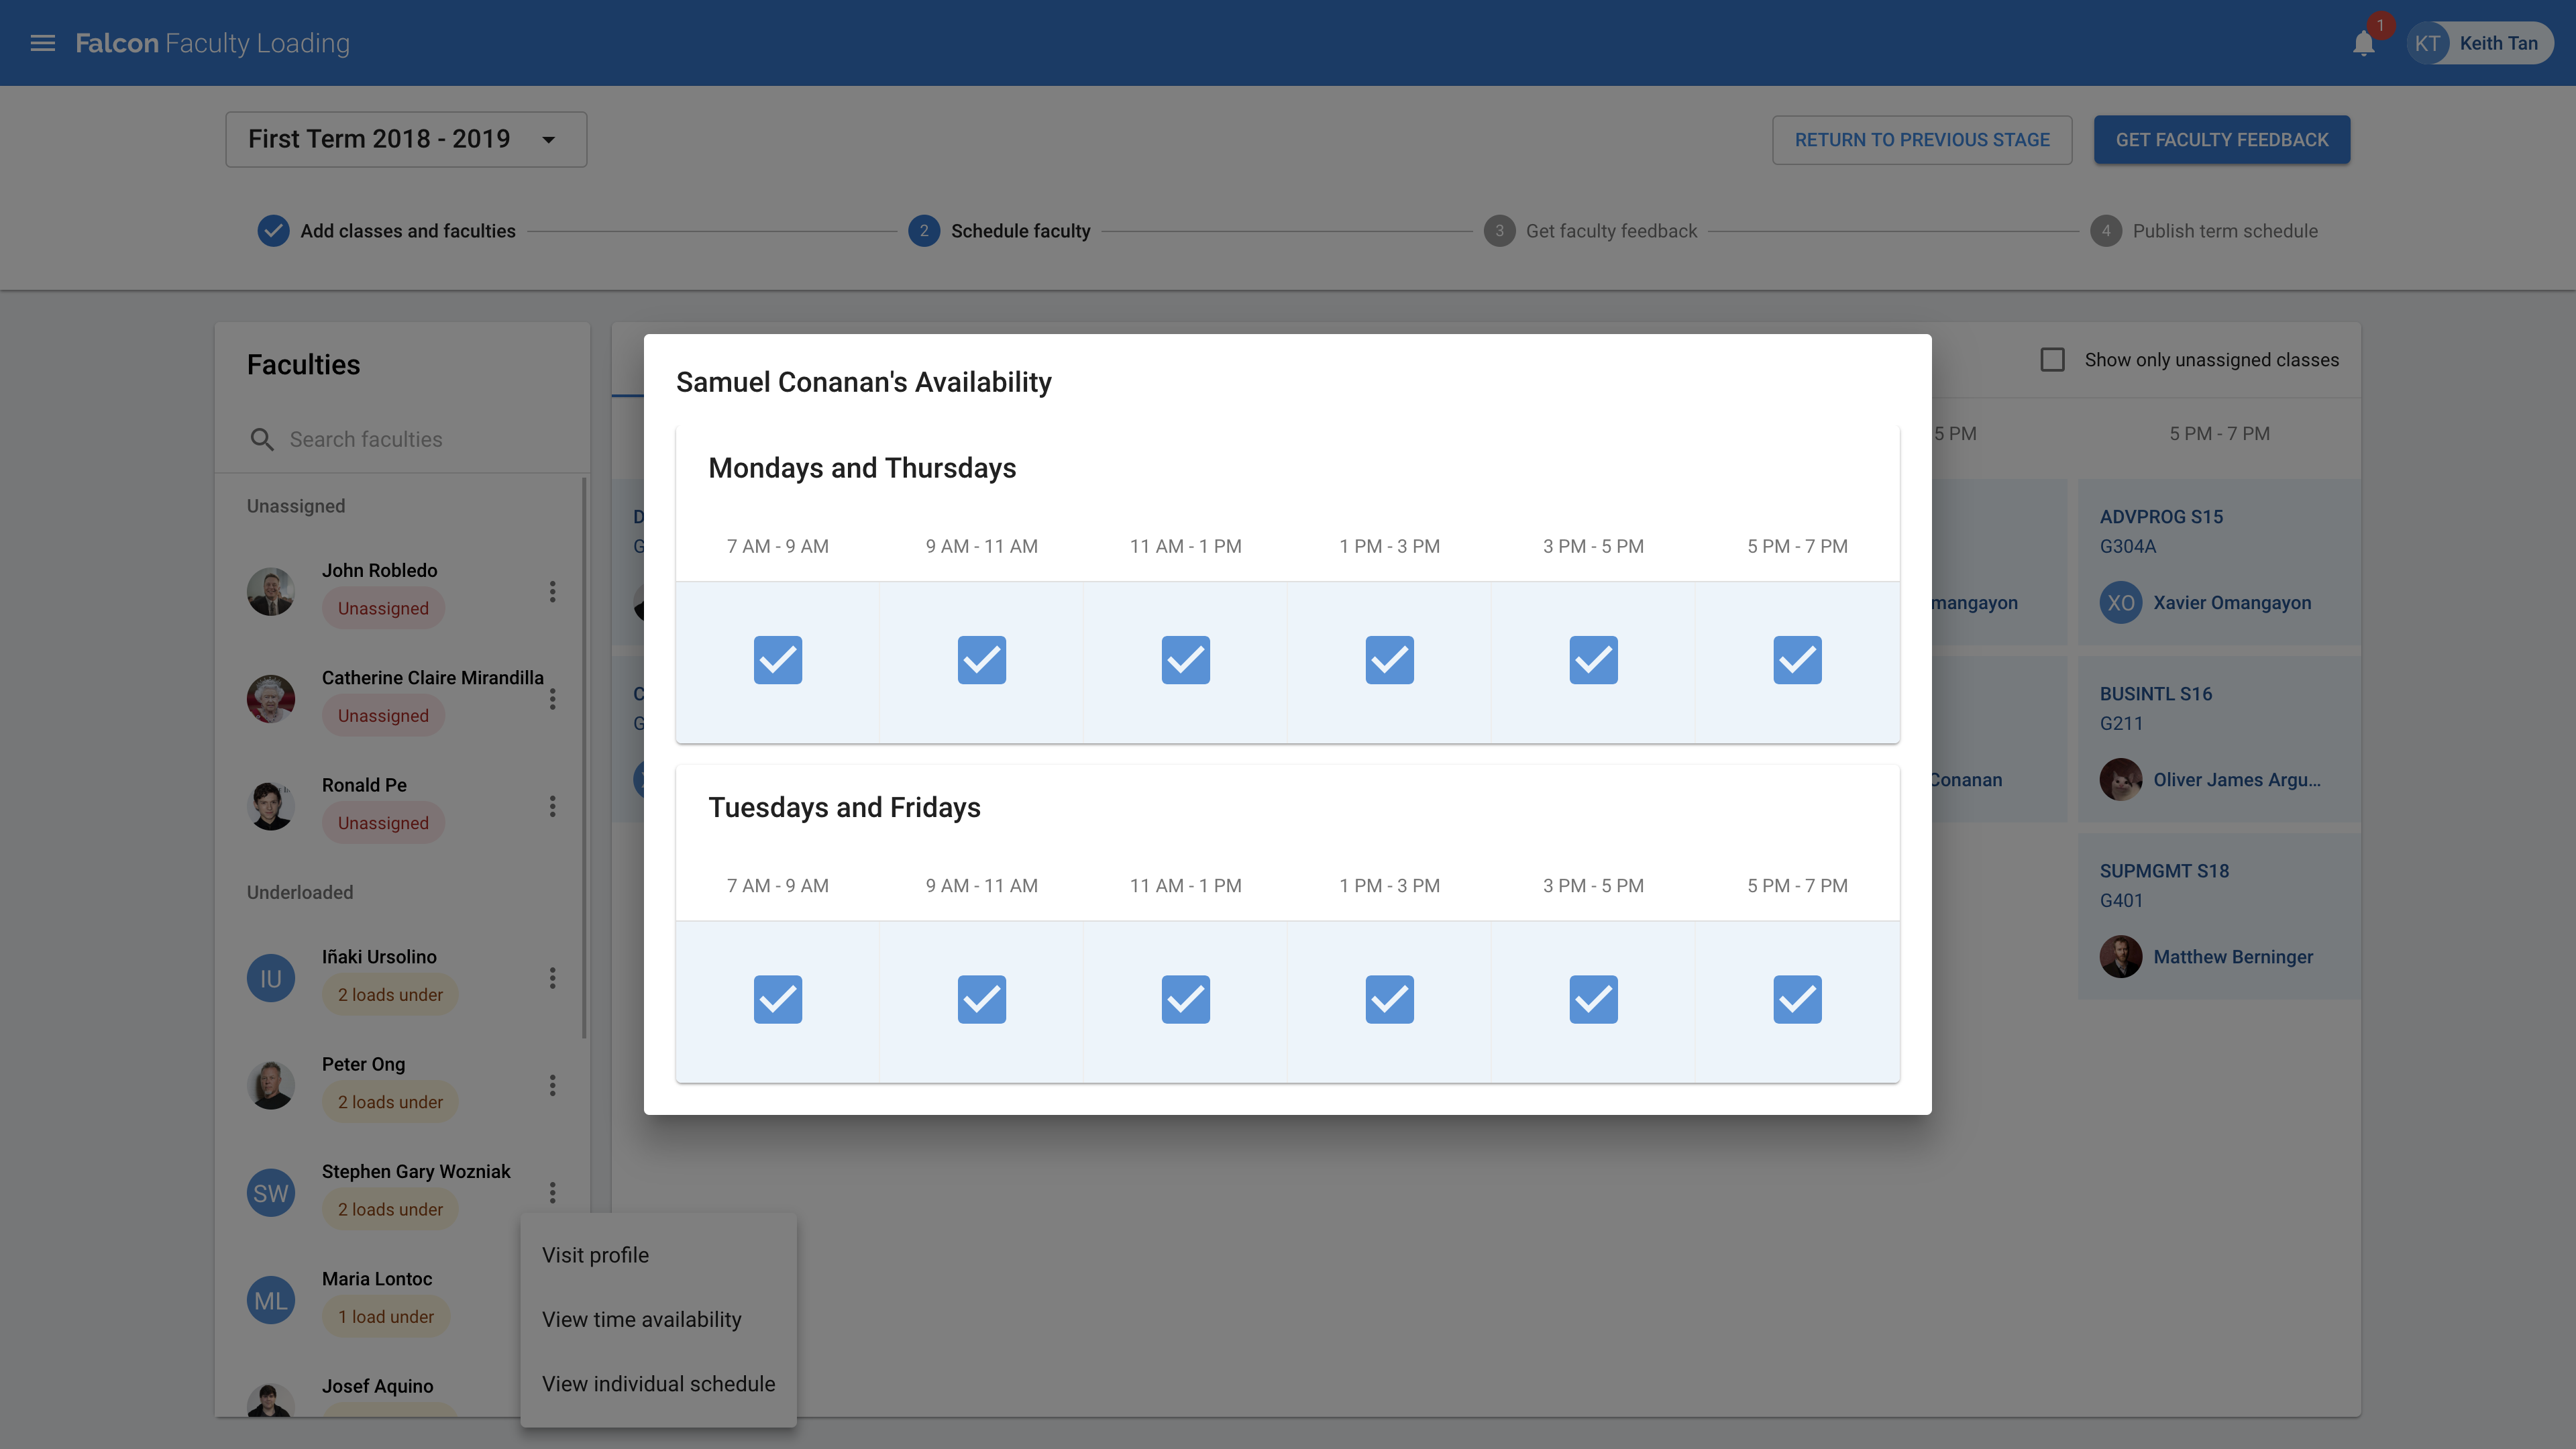
\includegraphics[width=\linewidth]{figures/screen_specifications/faculty_loading_screens/time_availability.png}
   \caption{Time Availability Screen}
   }
   
   \pagebreak
   
   
    \subsubsection{Individual Schedule}
    
    \field{Screen Name}{Individual Schedule}
    
    \field{File Name}{/pages/FacultyLoading/components/modals/FacultyScheduleModal/index.js}
    
    \field{Description} {Displays the schedule of each individual faculty member.}
    
    \field{Layout}{}
    
\makefigure{!h}{
   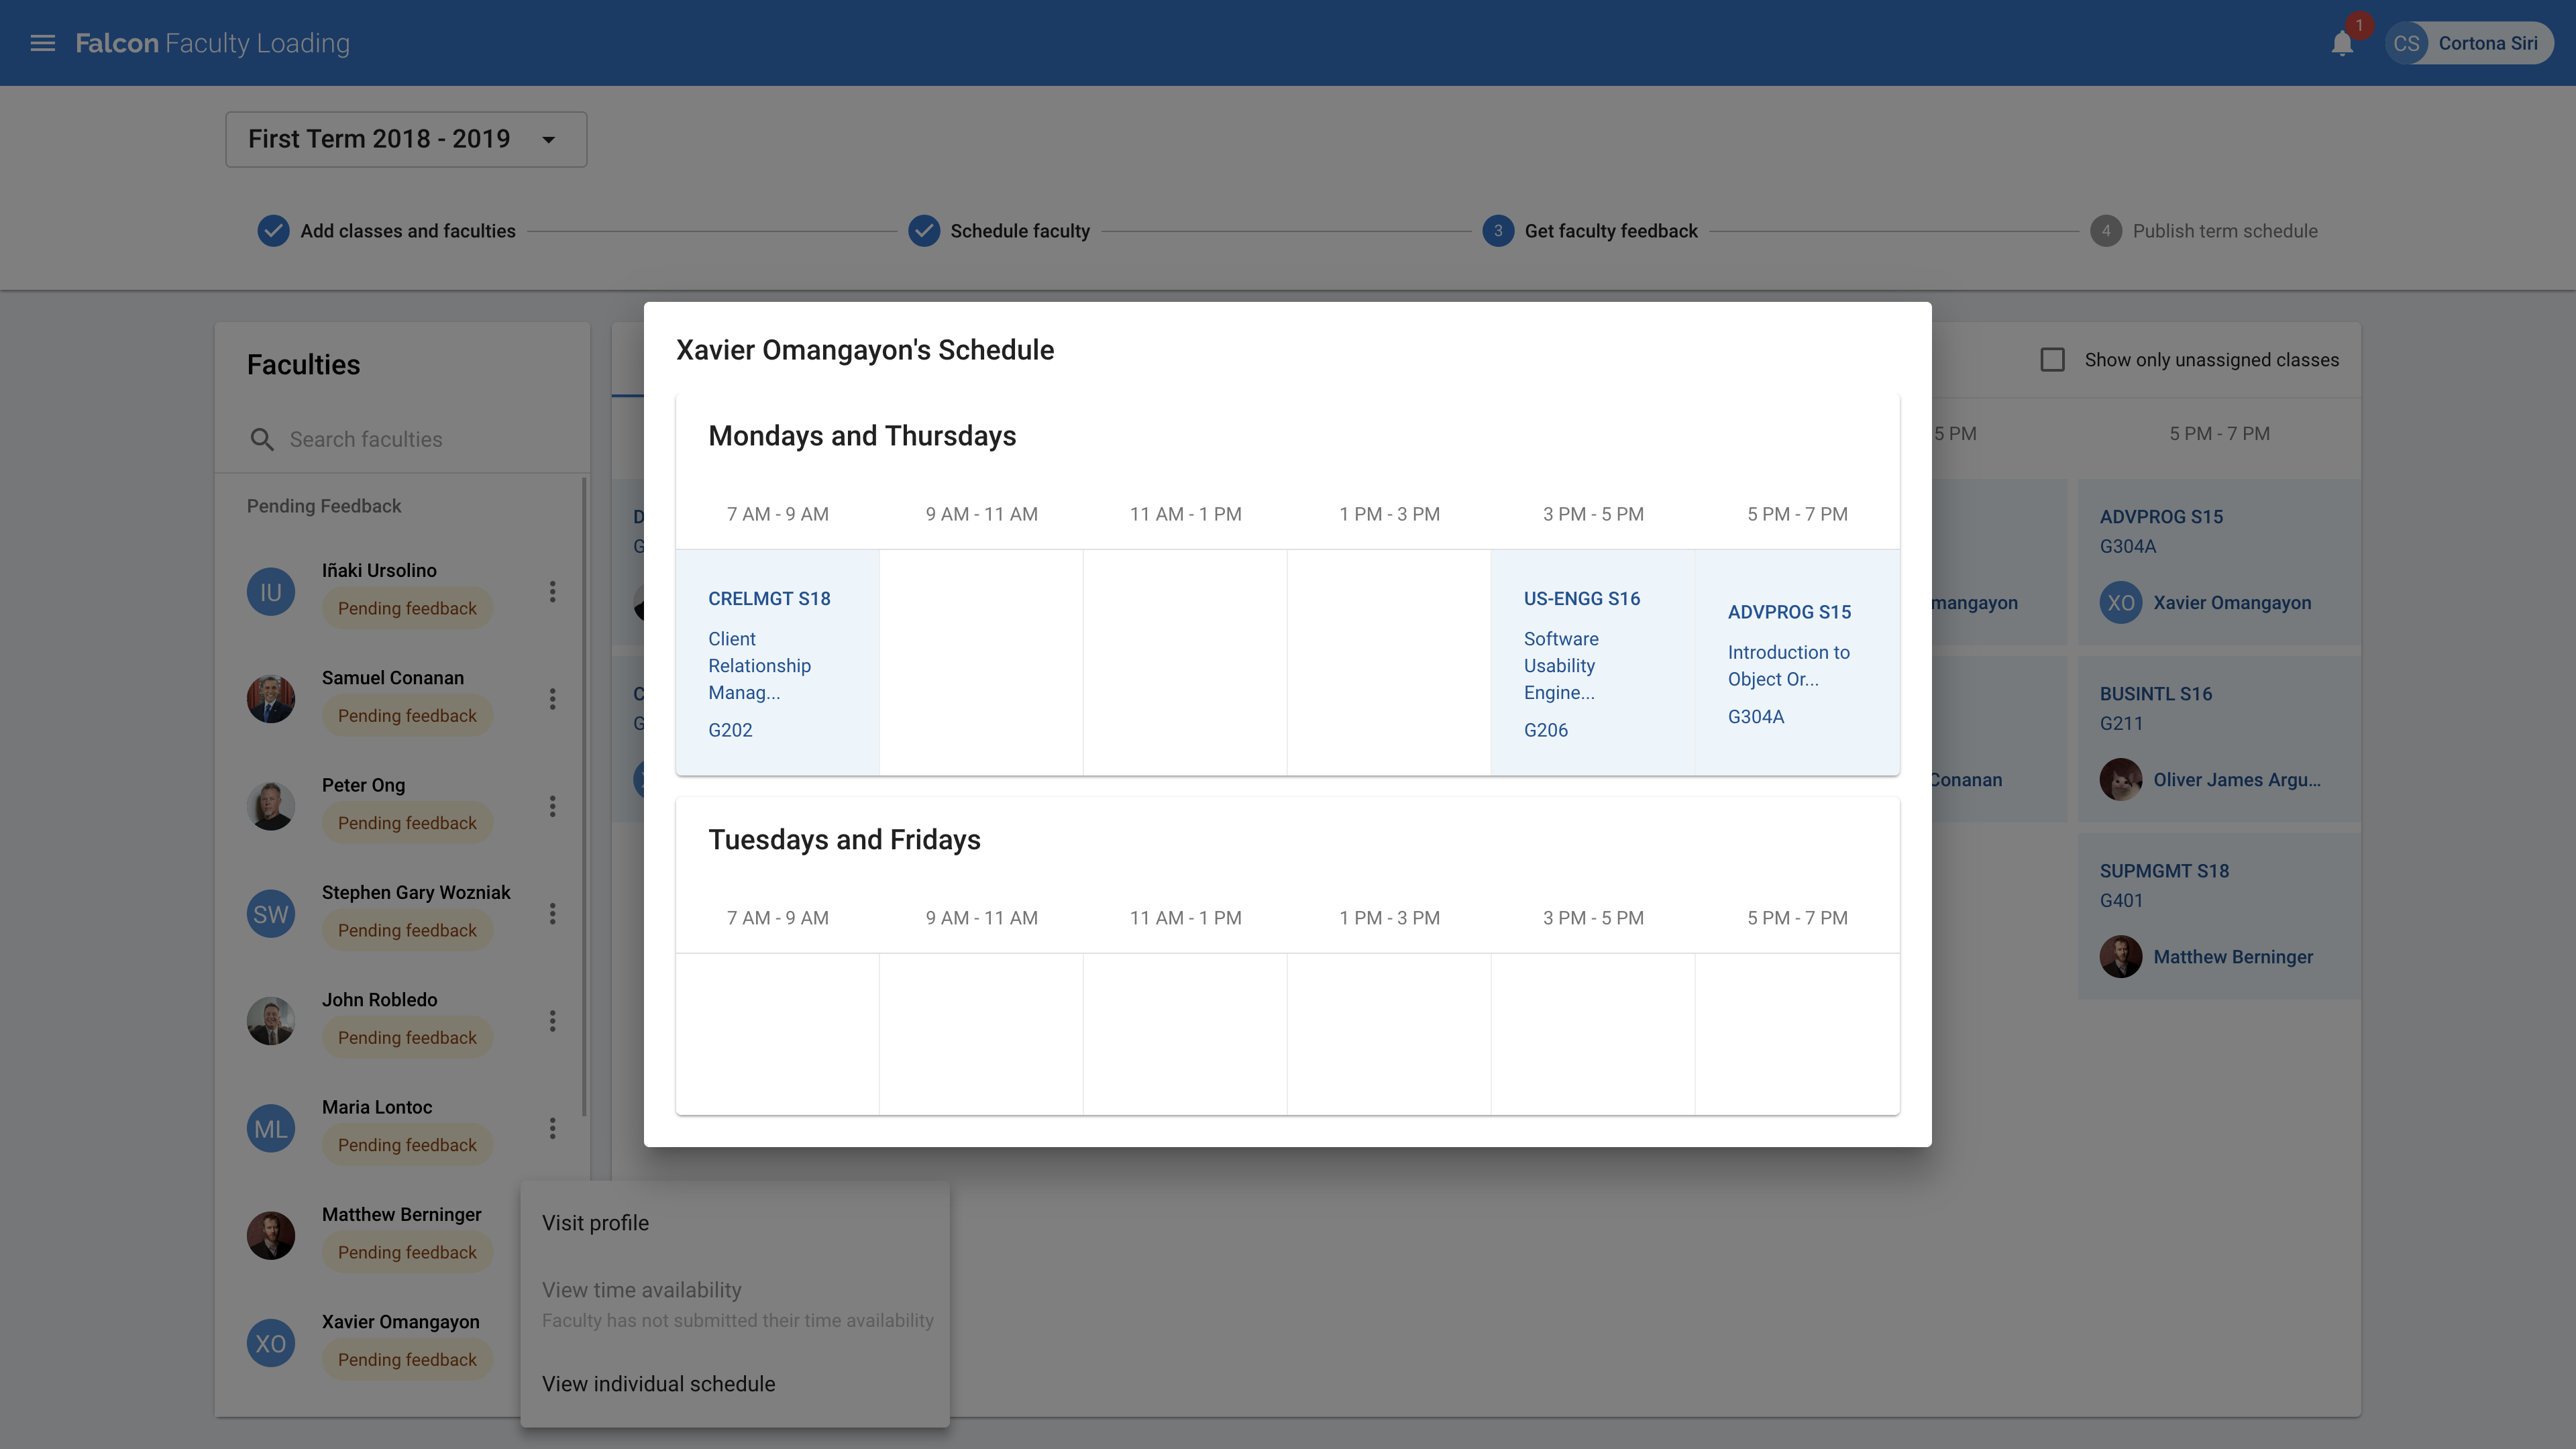
\includegraphics[width=\linewidth]{figures/screen_specifications/faculty_loading_screens/individual_schedule.png}
   \caption{Individual Schedule Screen}
   }
   
   \pagebreak
   
   
    \subsubsection{Schedule Print Preview}
    
    \field{Screen Name}{Schedule Print Preview}
    
    \field{File Name}{/pages/FacultyLoading/components/SchedulePrintPreview}
    
    \field{Description} {Displays the print preview for the schedules before printing.}
    
    \field{Layout}{}
    
\makefigure{!h}{
   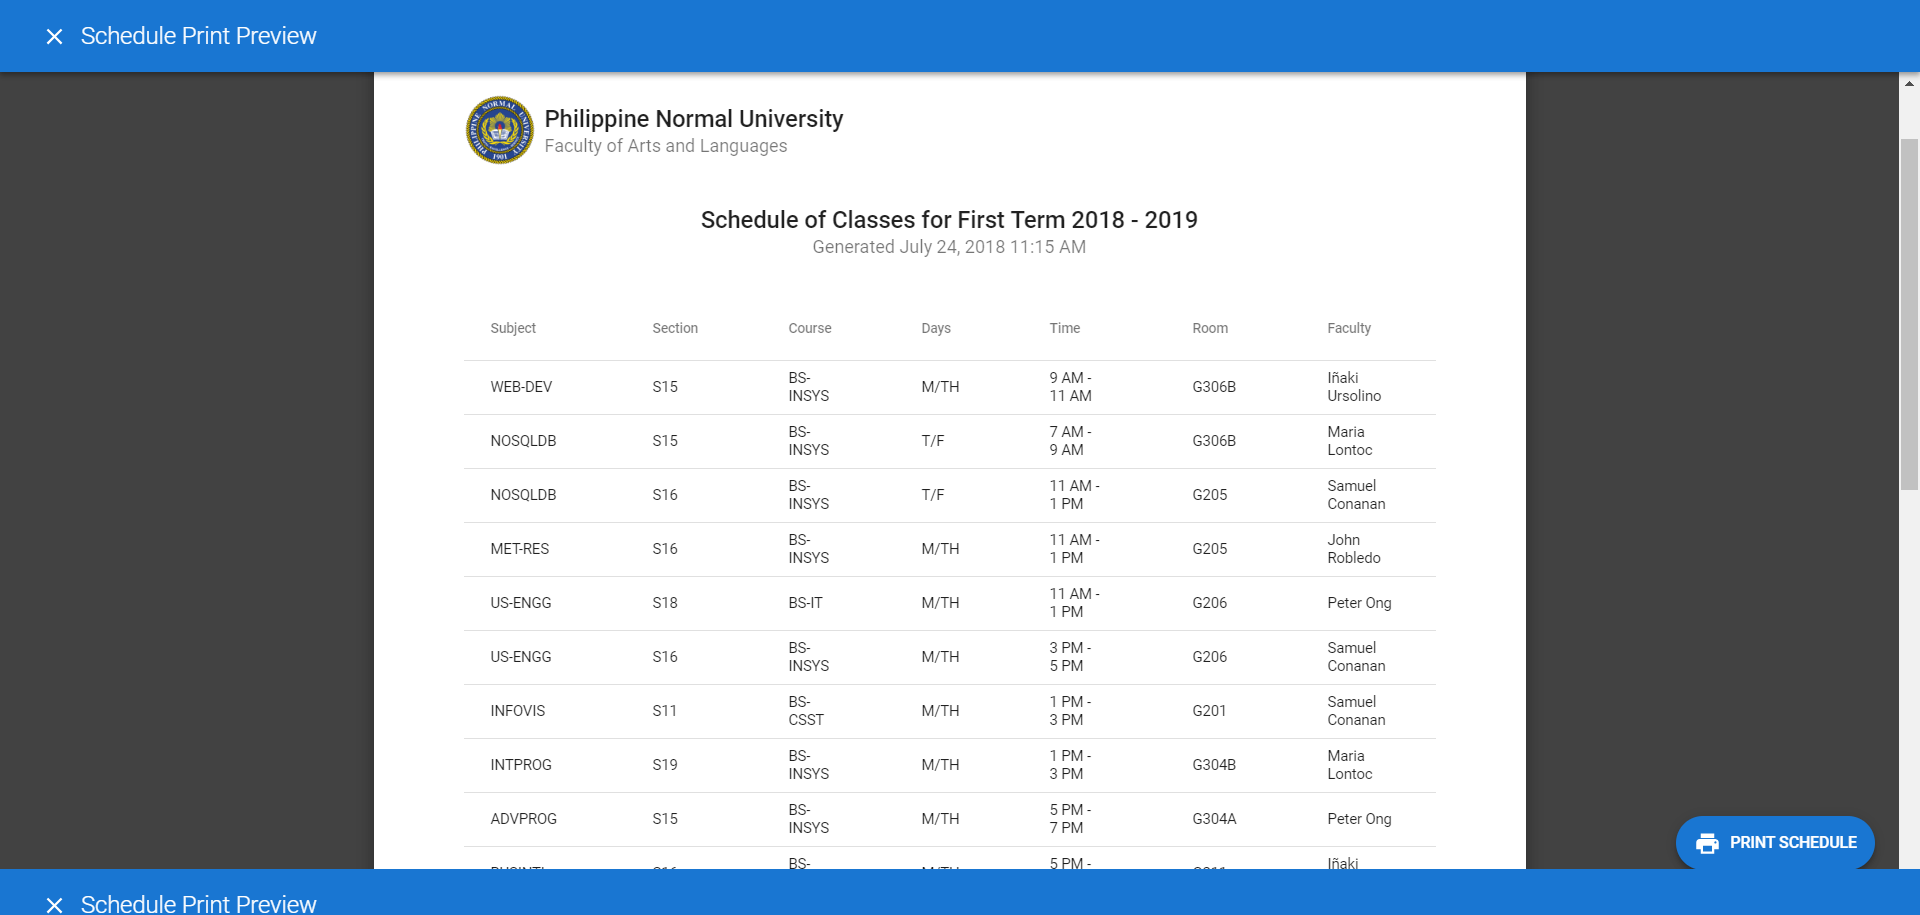
\includegraphics[width=\linewidth]{figures/screen_specifications/faculty_loading_screens/schedule_print.png}
   \caption{Schedule Print Preview Screen}
   }
   
   \pagebreak
    
\section{Form Specifications}

    \subsection{Faculty Profile}
    
    \subsubsection{Create User}
    
    \field{Form Name}{Create User}
    
    \field{Description}{For users to enter the basic information of their profile.}
    
    \field{Prepared by}{Clerk}
    
    \field{Volume and Frequency}{Created when a new faculty joins FAL.}
    
    \field{Layout}{}
    
    \pagebreak
    
\makefigure{!h}{
   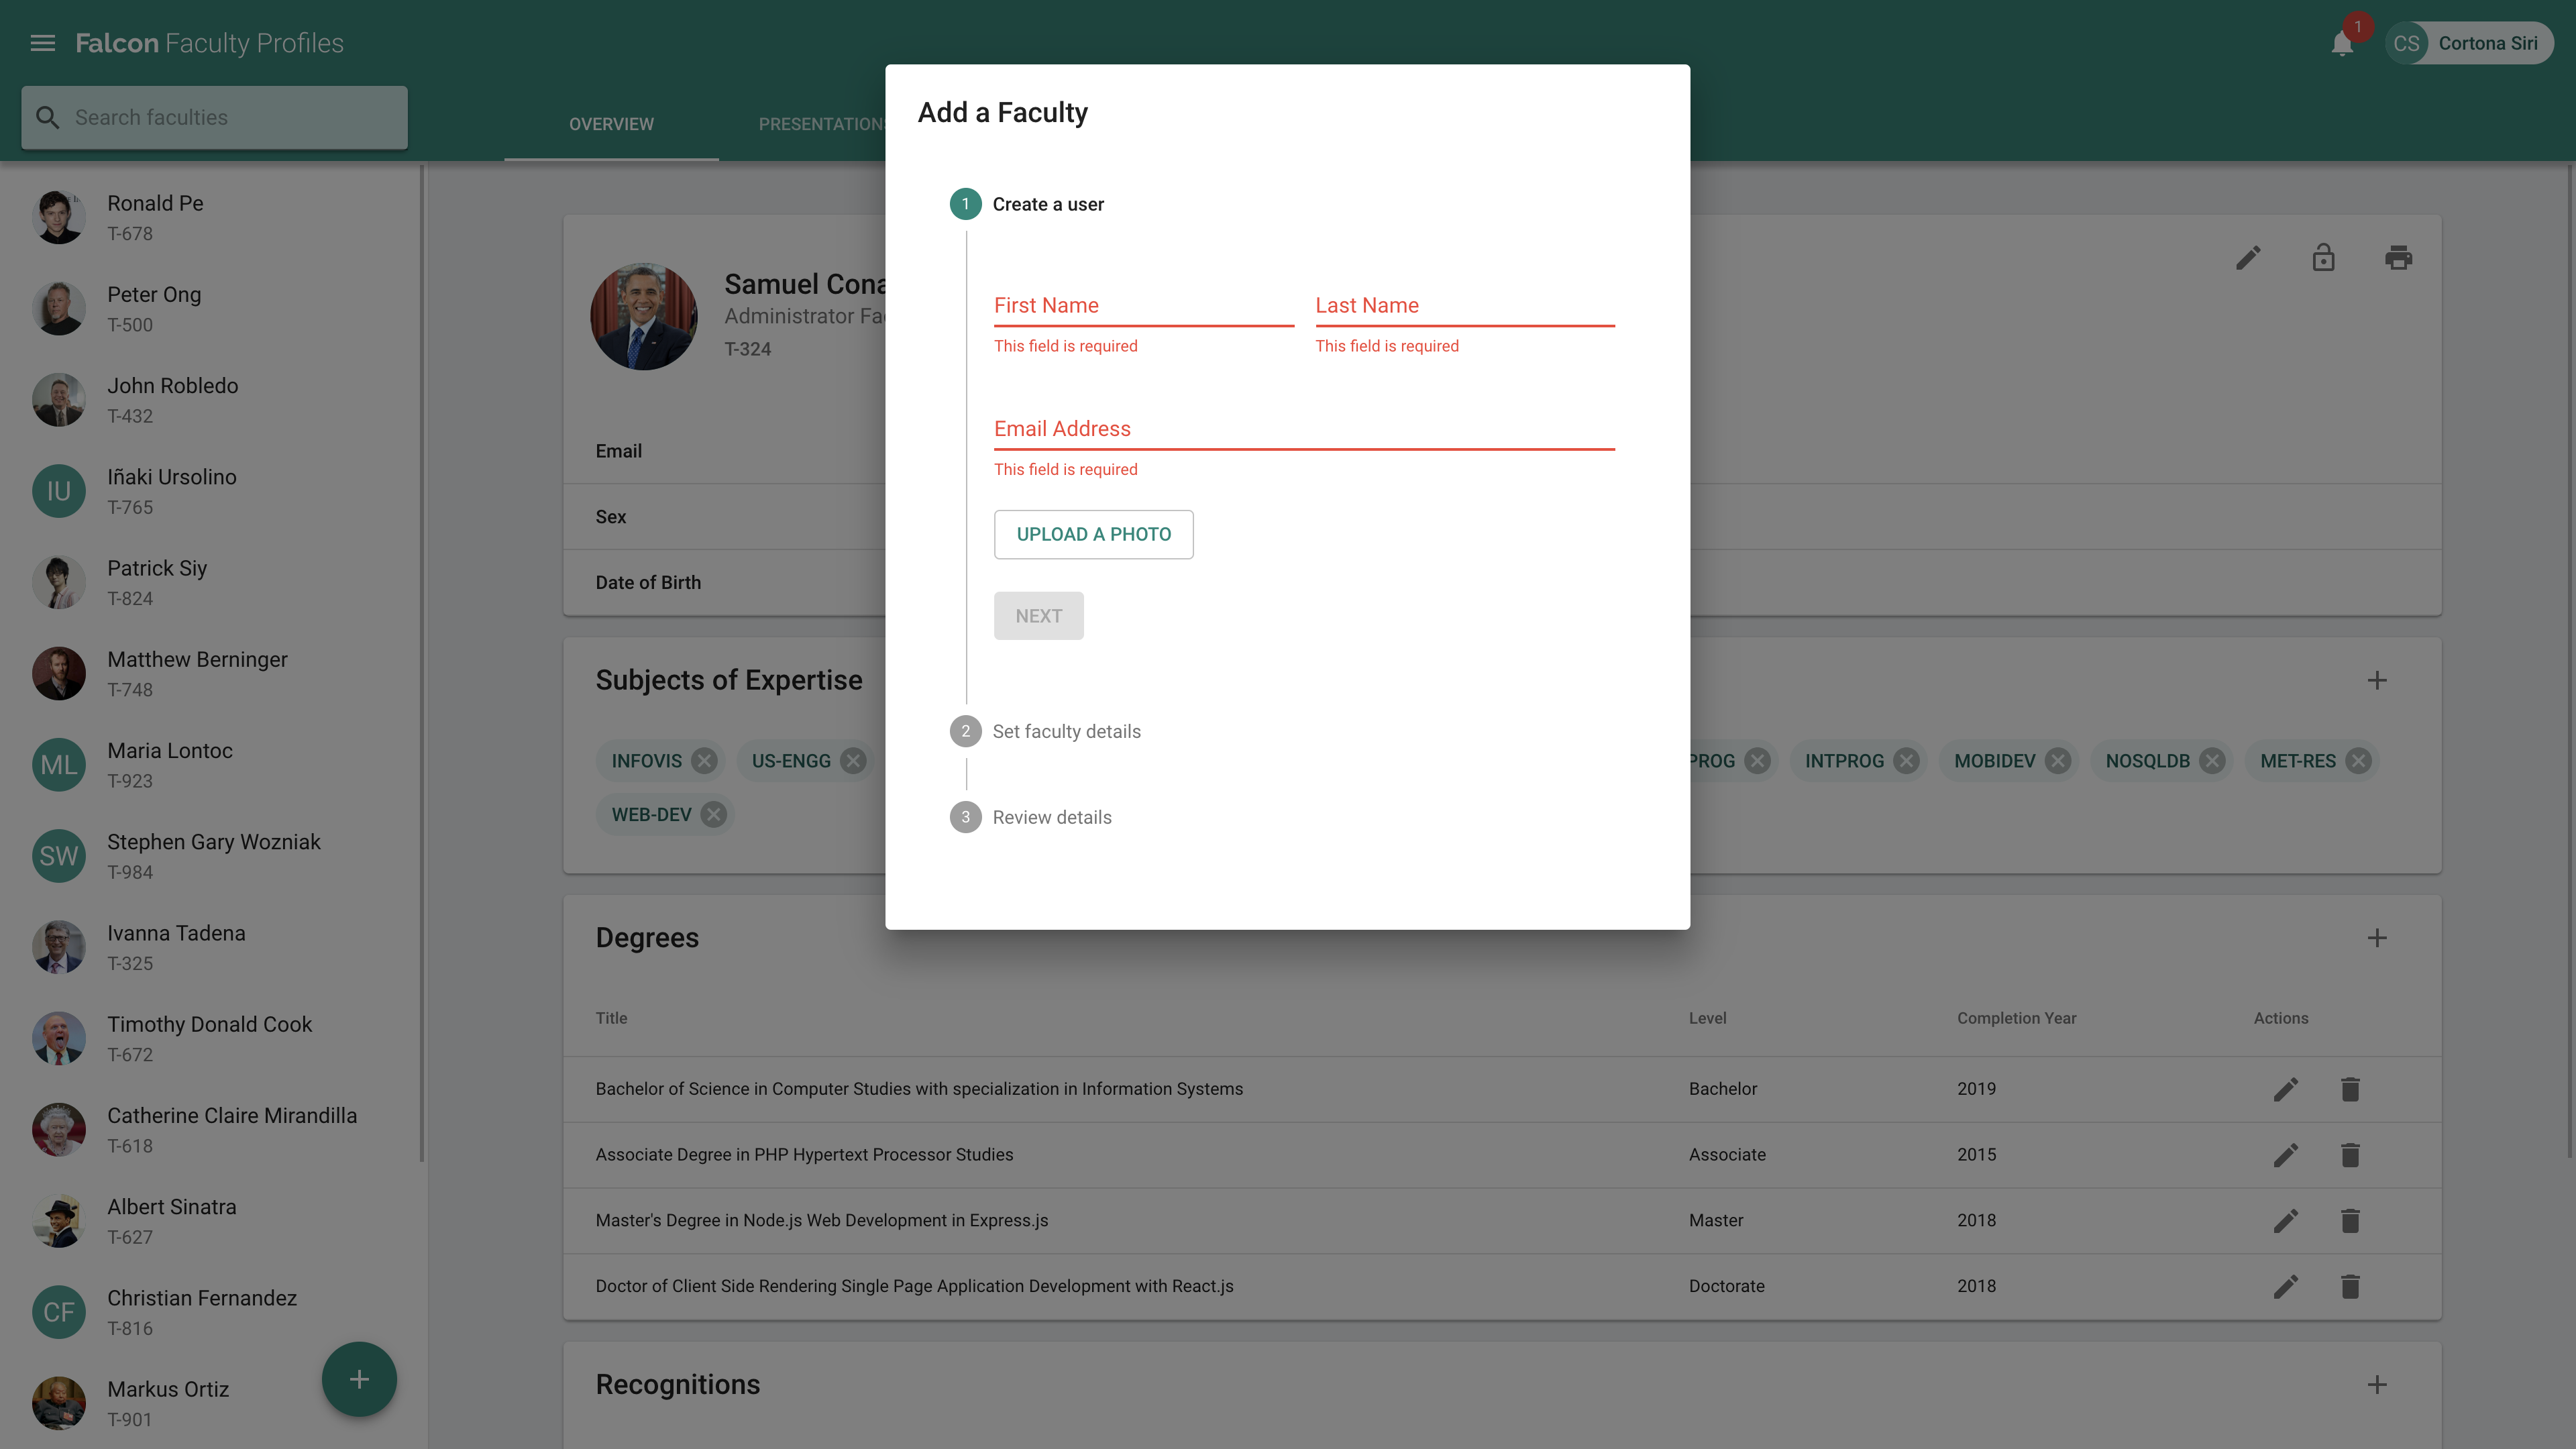
\includegraphics[width=\linewidth]{figures/form_specifications/create_user.png}
   \caption{Create User Screen}
}
    \pagebreak
    
    
    \subsubsection{Set Faculty}
    \field{Form Name} {Set Faculty}
    
    \field{Description}{For the faculty to input additional information into their profile.}
    
    \field{Prepared by} {Clerk}
    
    \field{Volume and Frequency}{Created when a new faculty joins FAL.}
    
    \field{Layout}{}
    
\makefigure{ht}{
   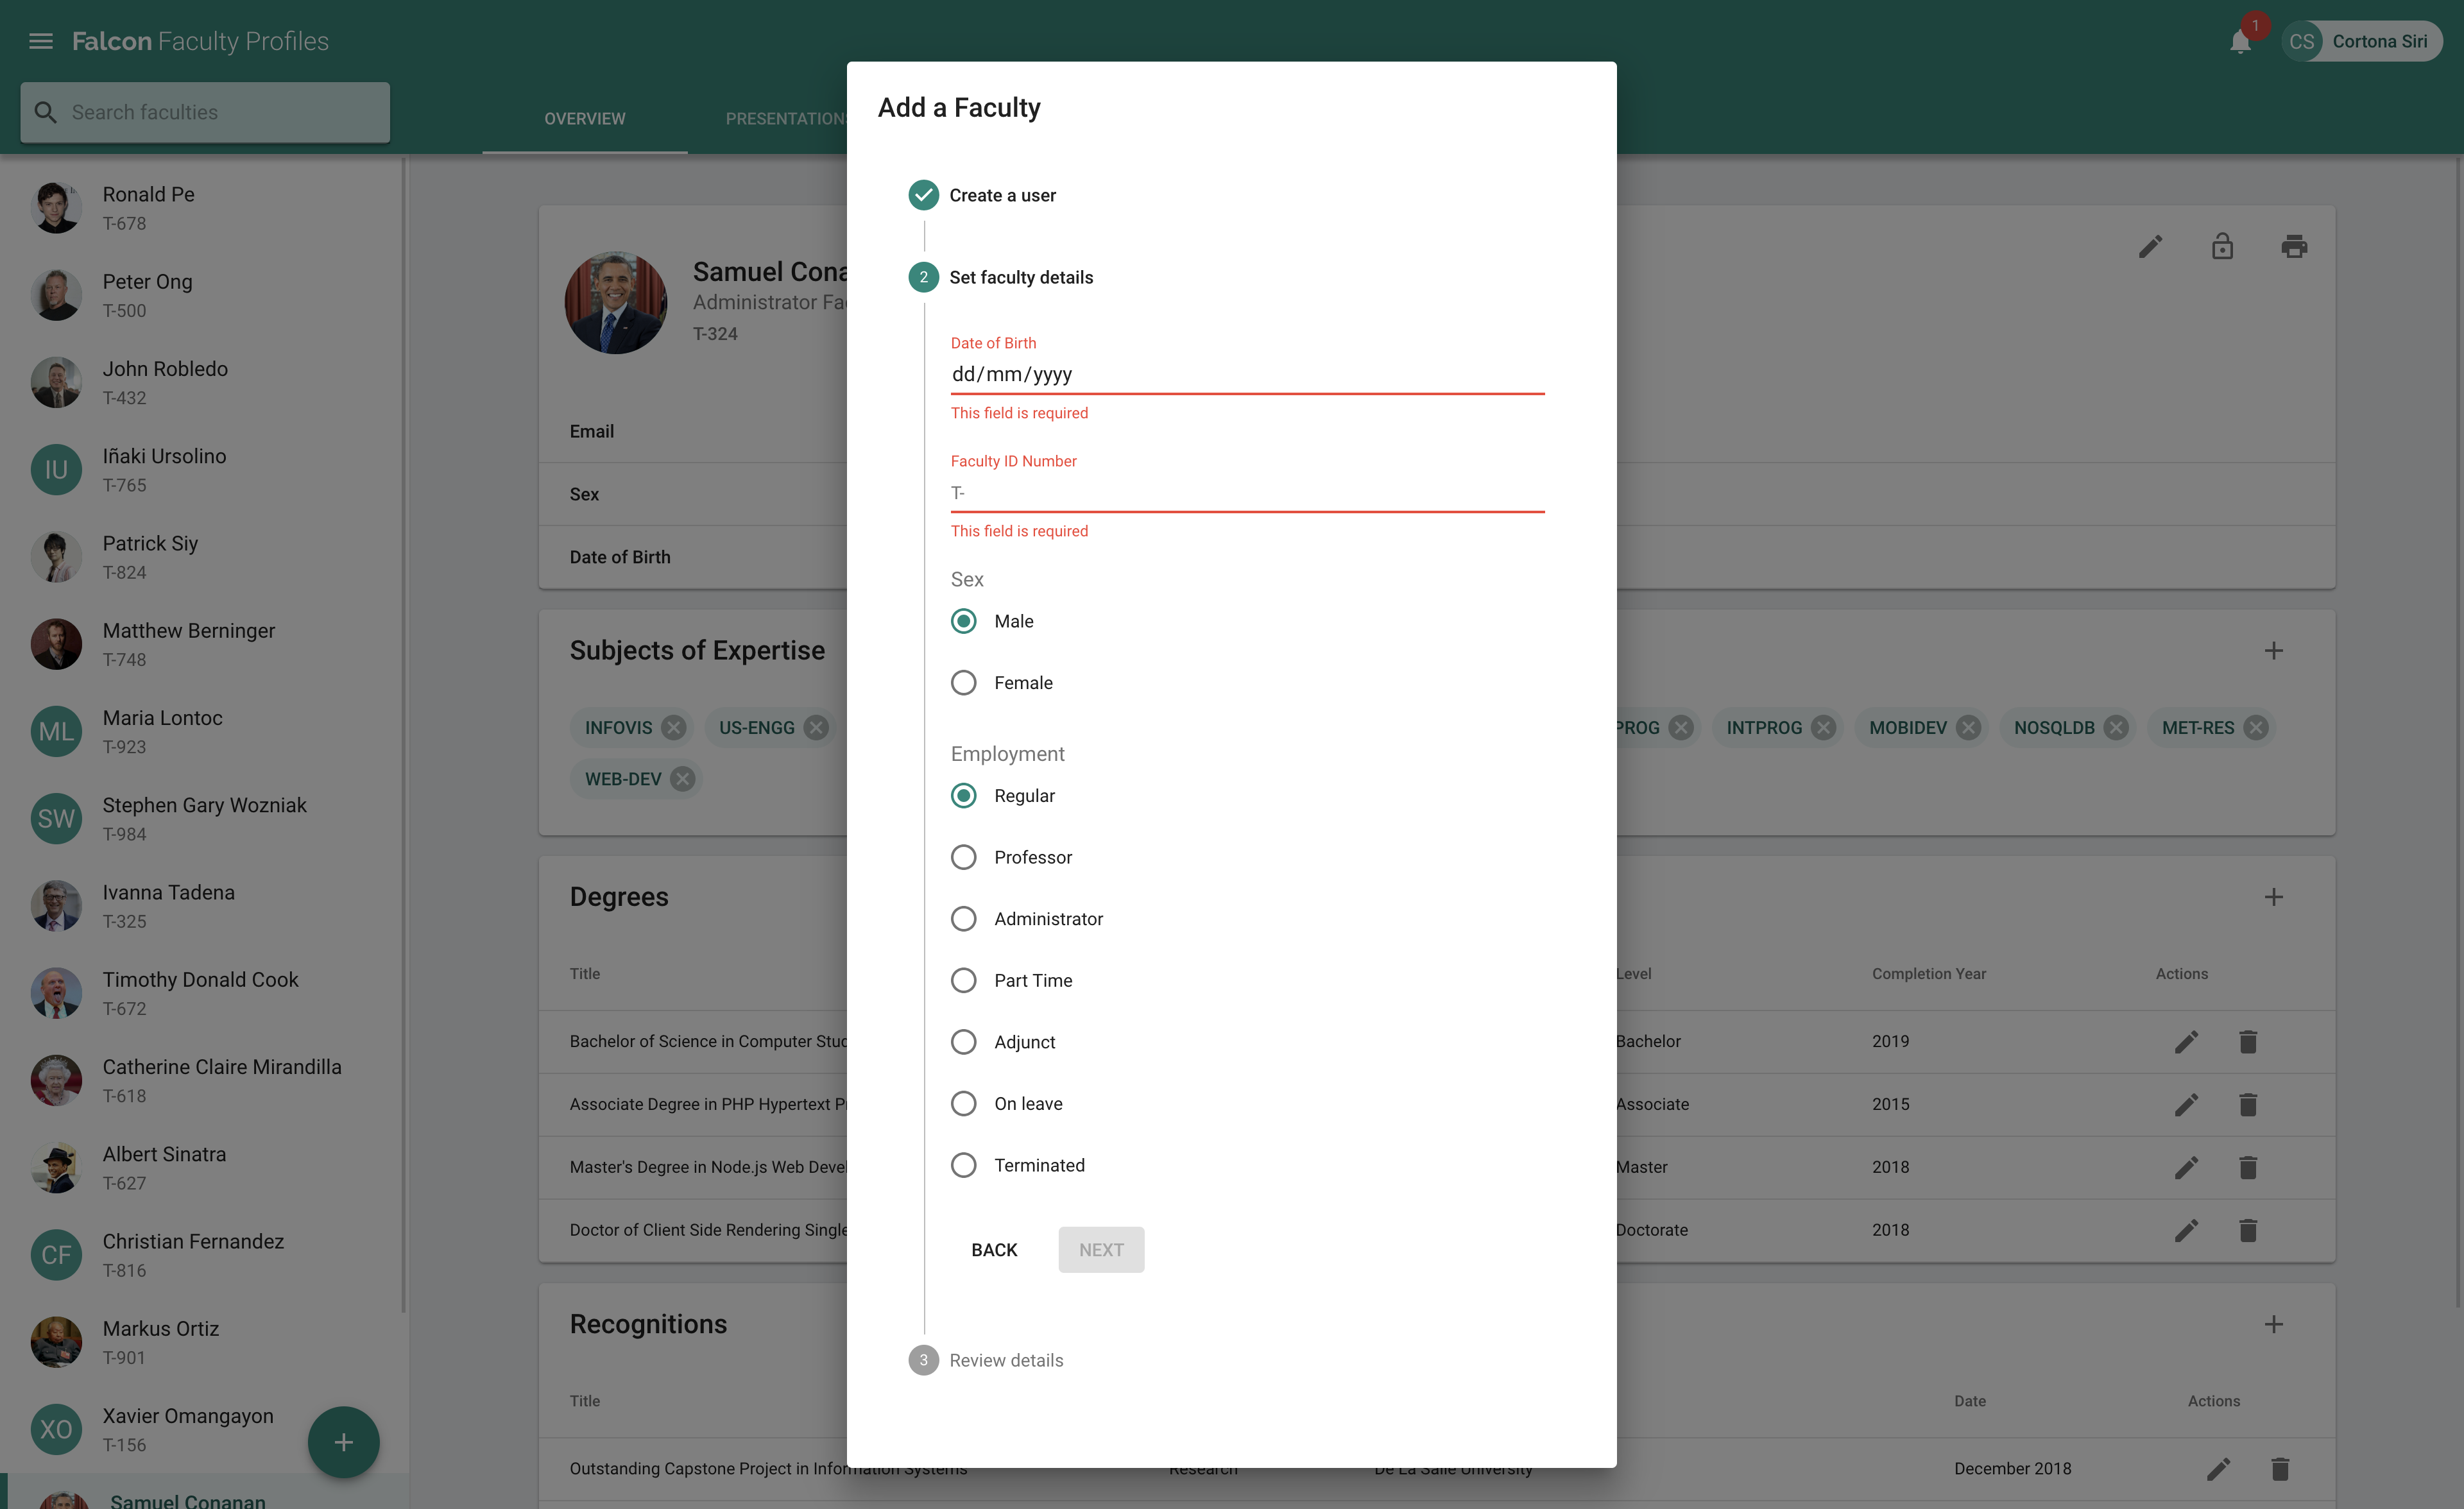
\includegraphics[width=\linewidth]{figures/form_specifications/set_faculty_details.png}
   \caption{Set Faculty Details Screen}
   }
   
   \pagebreak
    
    \subsubsection{Review Faculty}
    \field{Form Name}{Review Faculty}
    
    \field{Description}{For users review the information they inputted into the profile.}
    
    \field{Prepared by}{Clerk}
    
    \field{Volume and Frequency}{Created when a new faculty joins FAL.}
    
    \field{Layout}{}
    
\makefigure{!h}{
   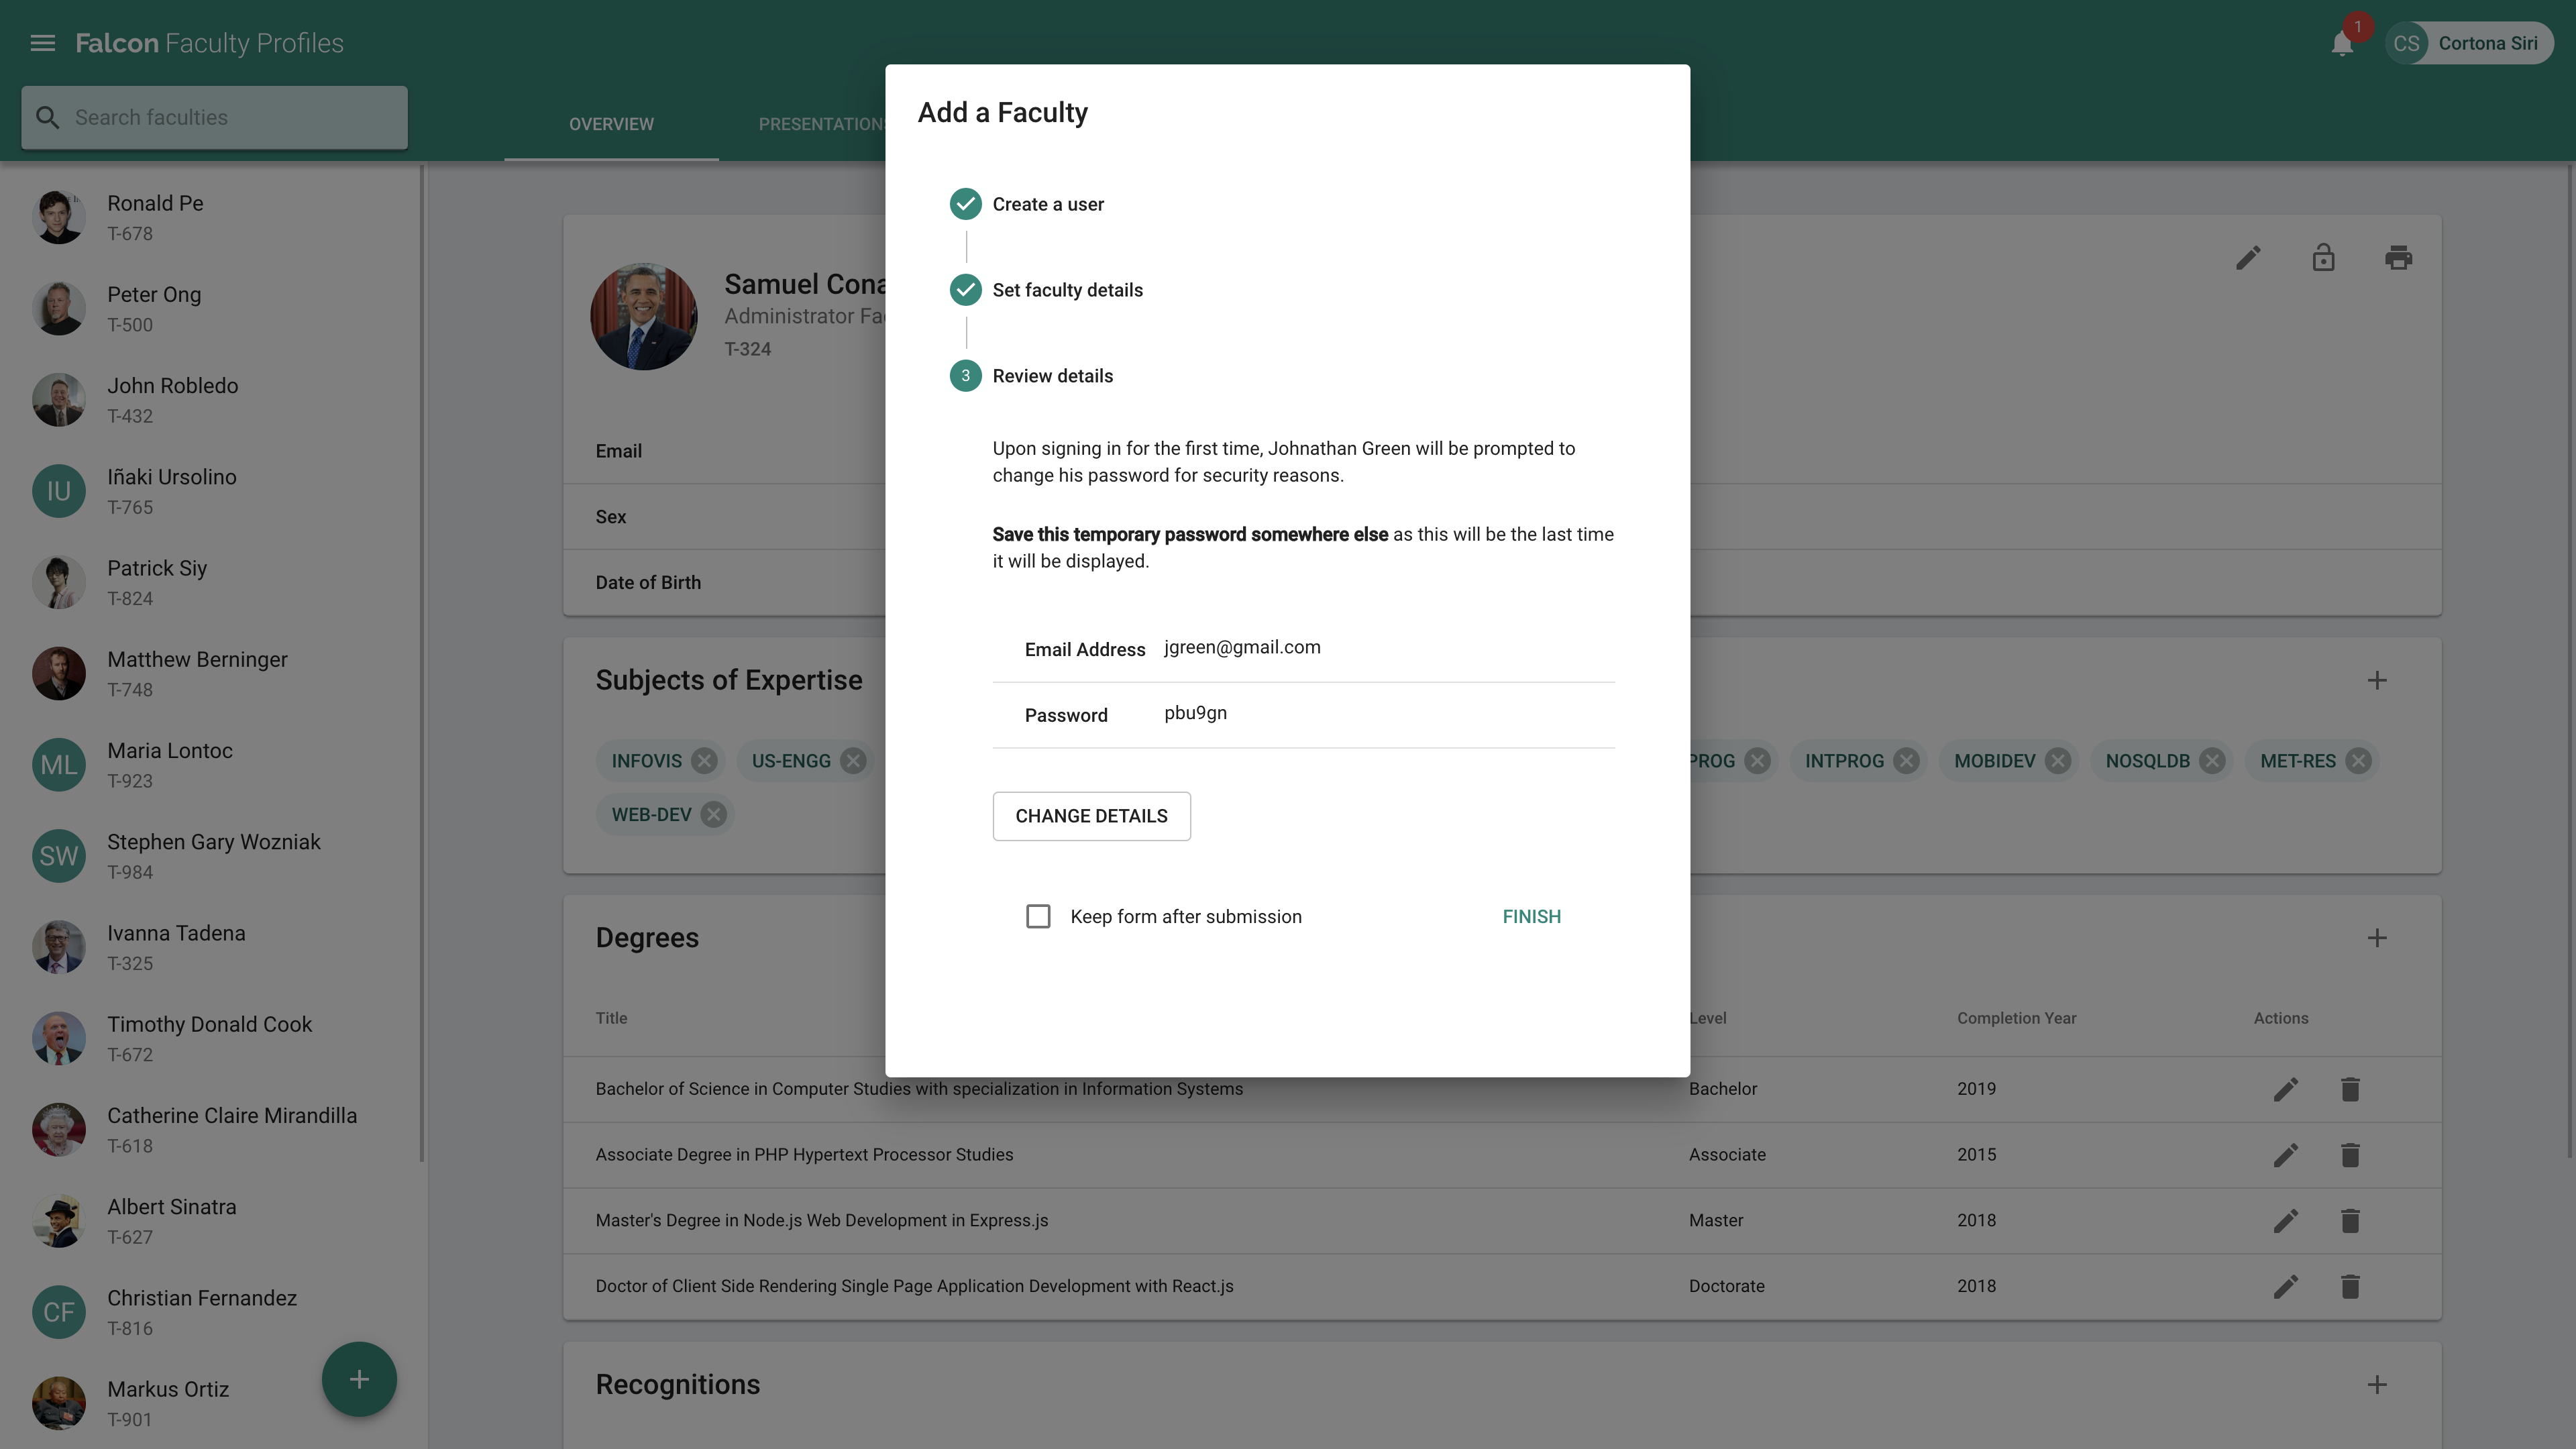
\includegraphics[width=\linewidth]{figures/form_specifications/review_details.png}
   \caption{Review Faculty Screen}
   }
   
   \pagebreak
    
    \subsubsection{Update Faculty}
    \field{Form Name}{Update Faculty}
    
    \field{Description}{For users to update the information in the faculty profile.}
    
    \field{Prepared by}{Clerk}
    
    \field{Volume and Frequency}{When information on the faculty profile needs to be updated}
    
    \field{Layout}{}
    
\makefigure{!h}{
   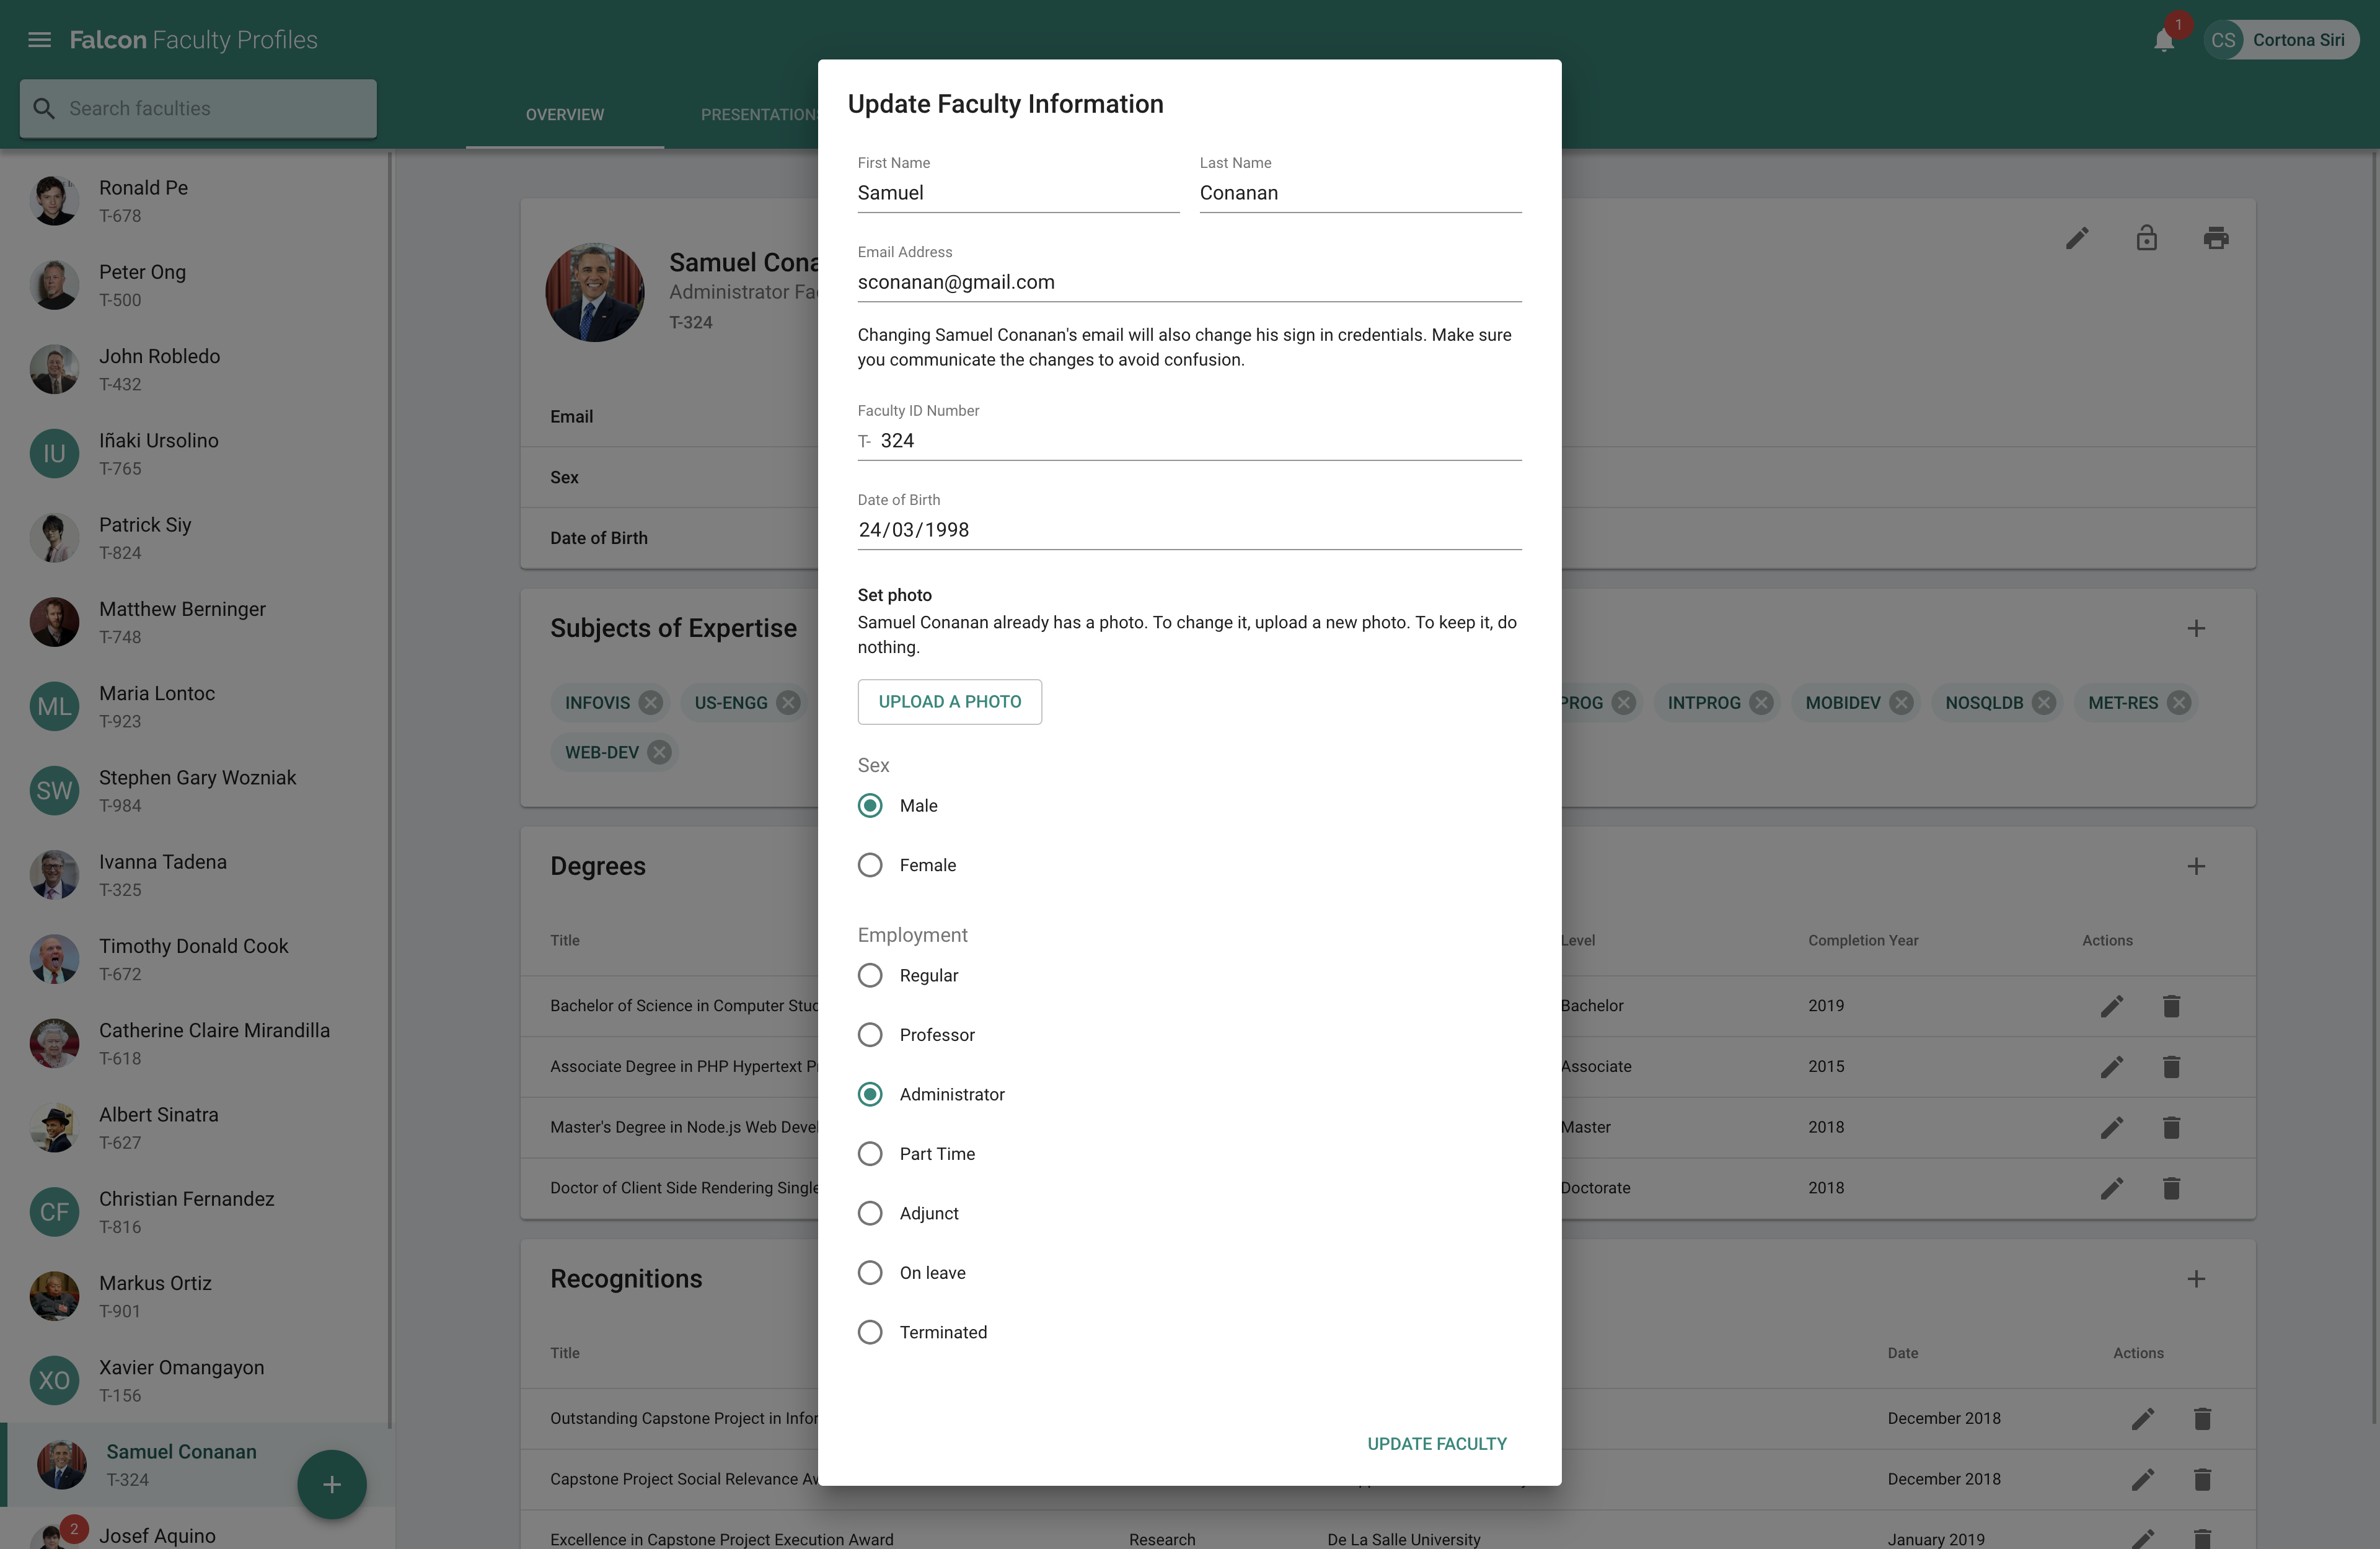
\includegraphics[width=\linewidth]{figures/form_specifications/update_faculty.png}
   \caption{Update Faculty Screen}
   }
   \pagebreak
    
    \subsubsection{Add/Update Degree}
    \field{Form Name}{Add/Update Degree}
    
    \field{Description}{For users to add a new degree or update the details of an existing degree.}
    
    \field{Prepared by}{Clerk}
    
    \field{Volume and Frequency}{Added when the faculty earns a new degree, or when faculty has requested to add or update their degree.}
    
    \field{Layout}{}
    
\makefigure{!h}{
   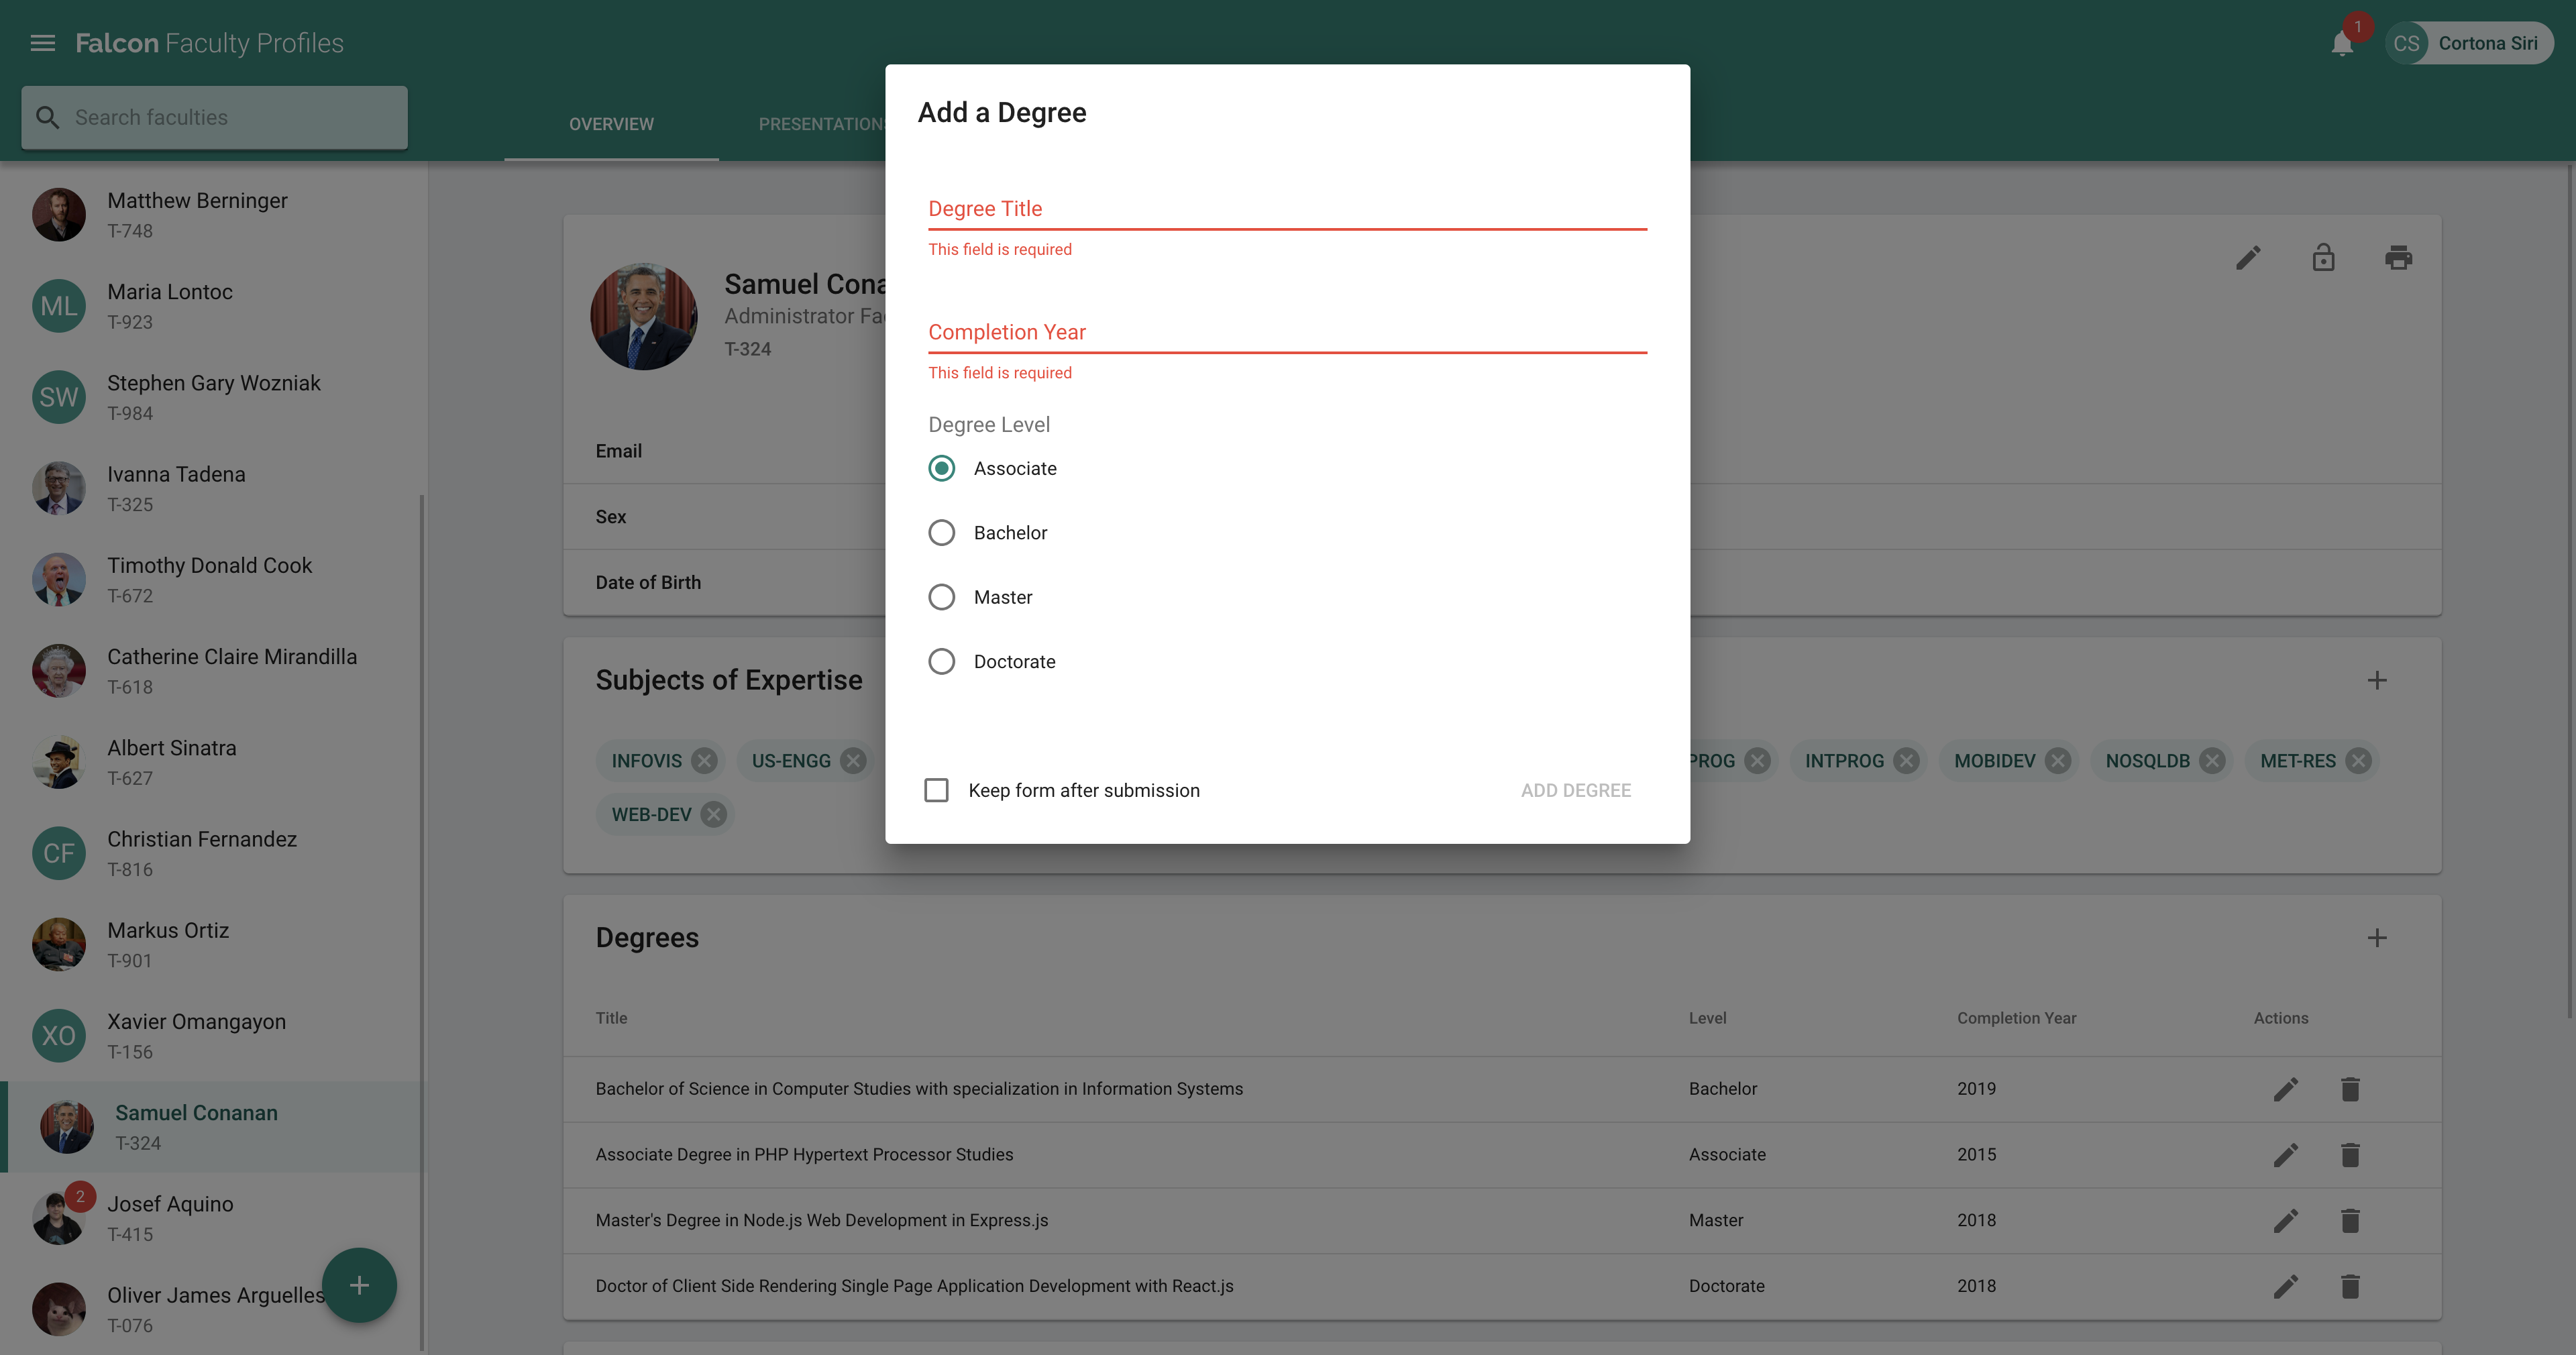
\includegraphics[width=\linewidth]{figures/form_specifications/add_degree.png}
   \caption{Add/Update Degree Screen}
   }
    
    \pagebreak
    
    \subsubsection{Add/Update Recognition}
    \field{Form Name}{Add/Update Recognition}
    
    \field{Description}{For the clerk to add a new degree or update the details of an existing degree.}
    
    \field{Prepared by}{Clerk}
    
    \field{Volume and Frequency}{Added when the faculty earns a new recognition, or when faculty has requested to add or update their recognitions.}
    
    \field{Layout}{}
    
\makefigure{!h}{
   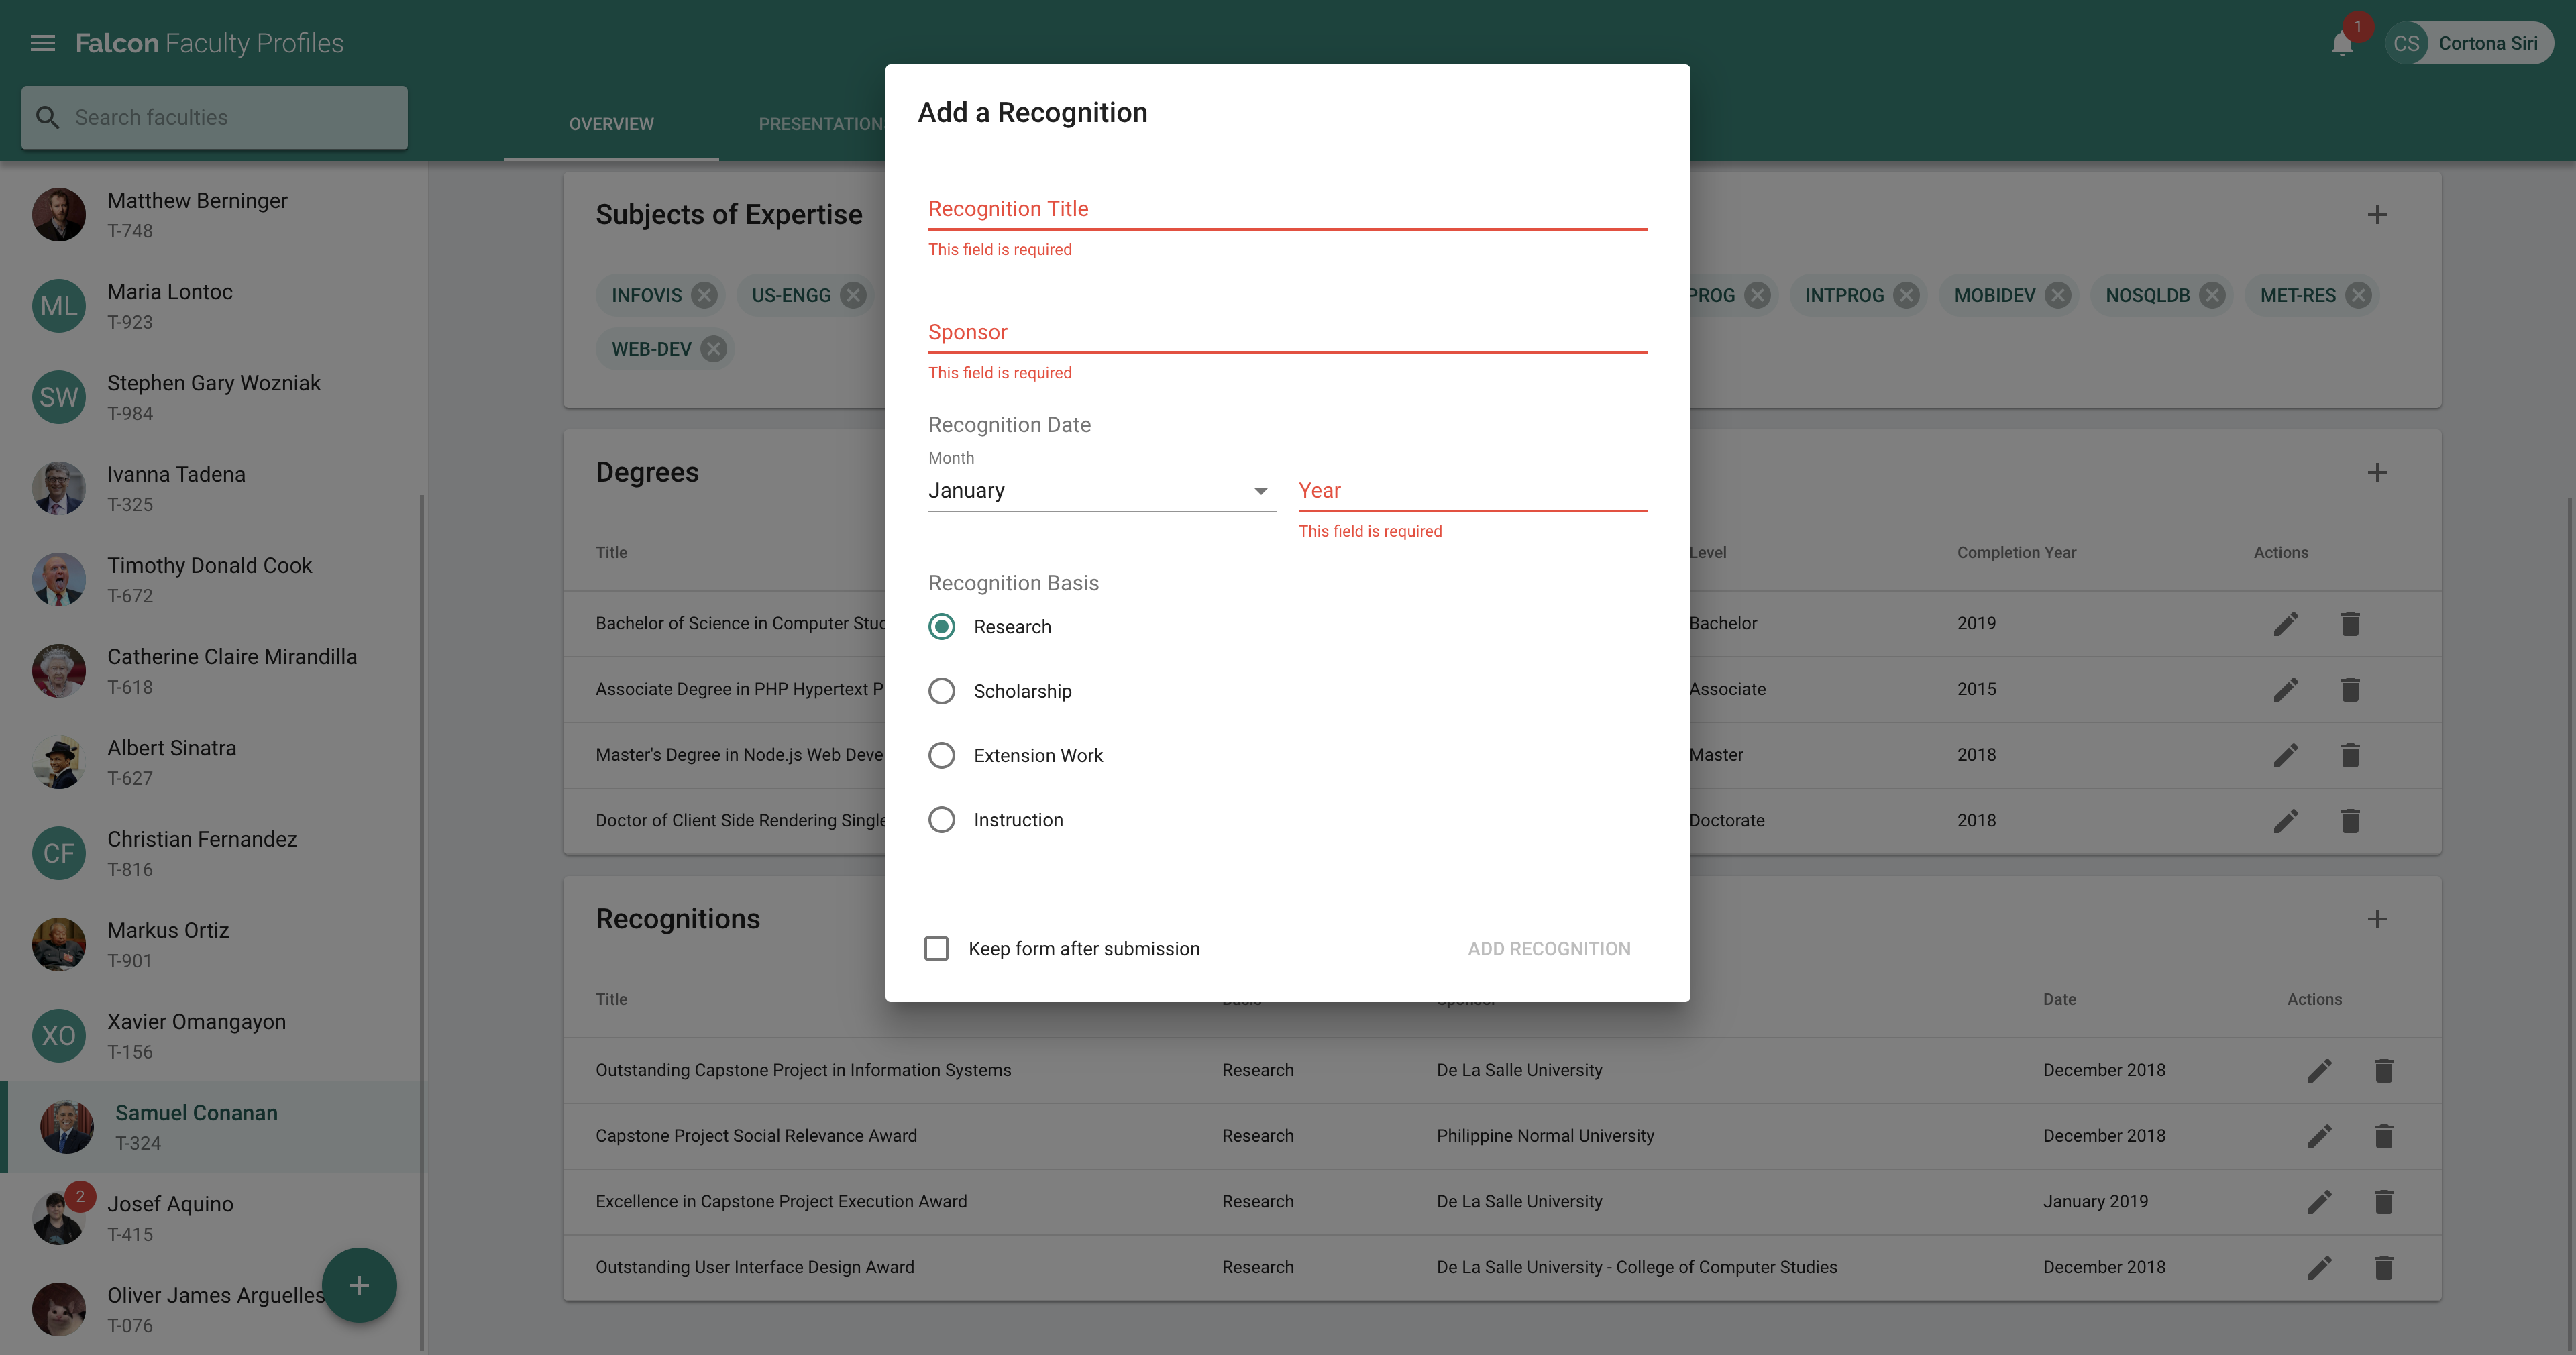
\includegraphics[width=\linewidth]{figures/form_specifications/add_recognition.png}
   \caption{Add/Update Recognition Screen}
   }
    
    \pagebreak
    
    \subsubsection{Set Expertise}
    \field{Form Name}{Set Subjects of Expertise}
    
    \field{Description}{For the clerk to set the subjects the faculty are experts in teaching.}
    
    \field{Prepared by}{Clerk}
    
    \field{Volume and Frequency}{Done when the faculty has earned a new expertise on a subject.}
    
    \field{Layout}{}
    
\makefigure{!h}{
   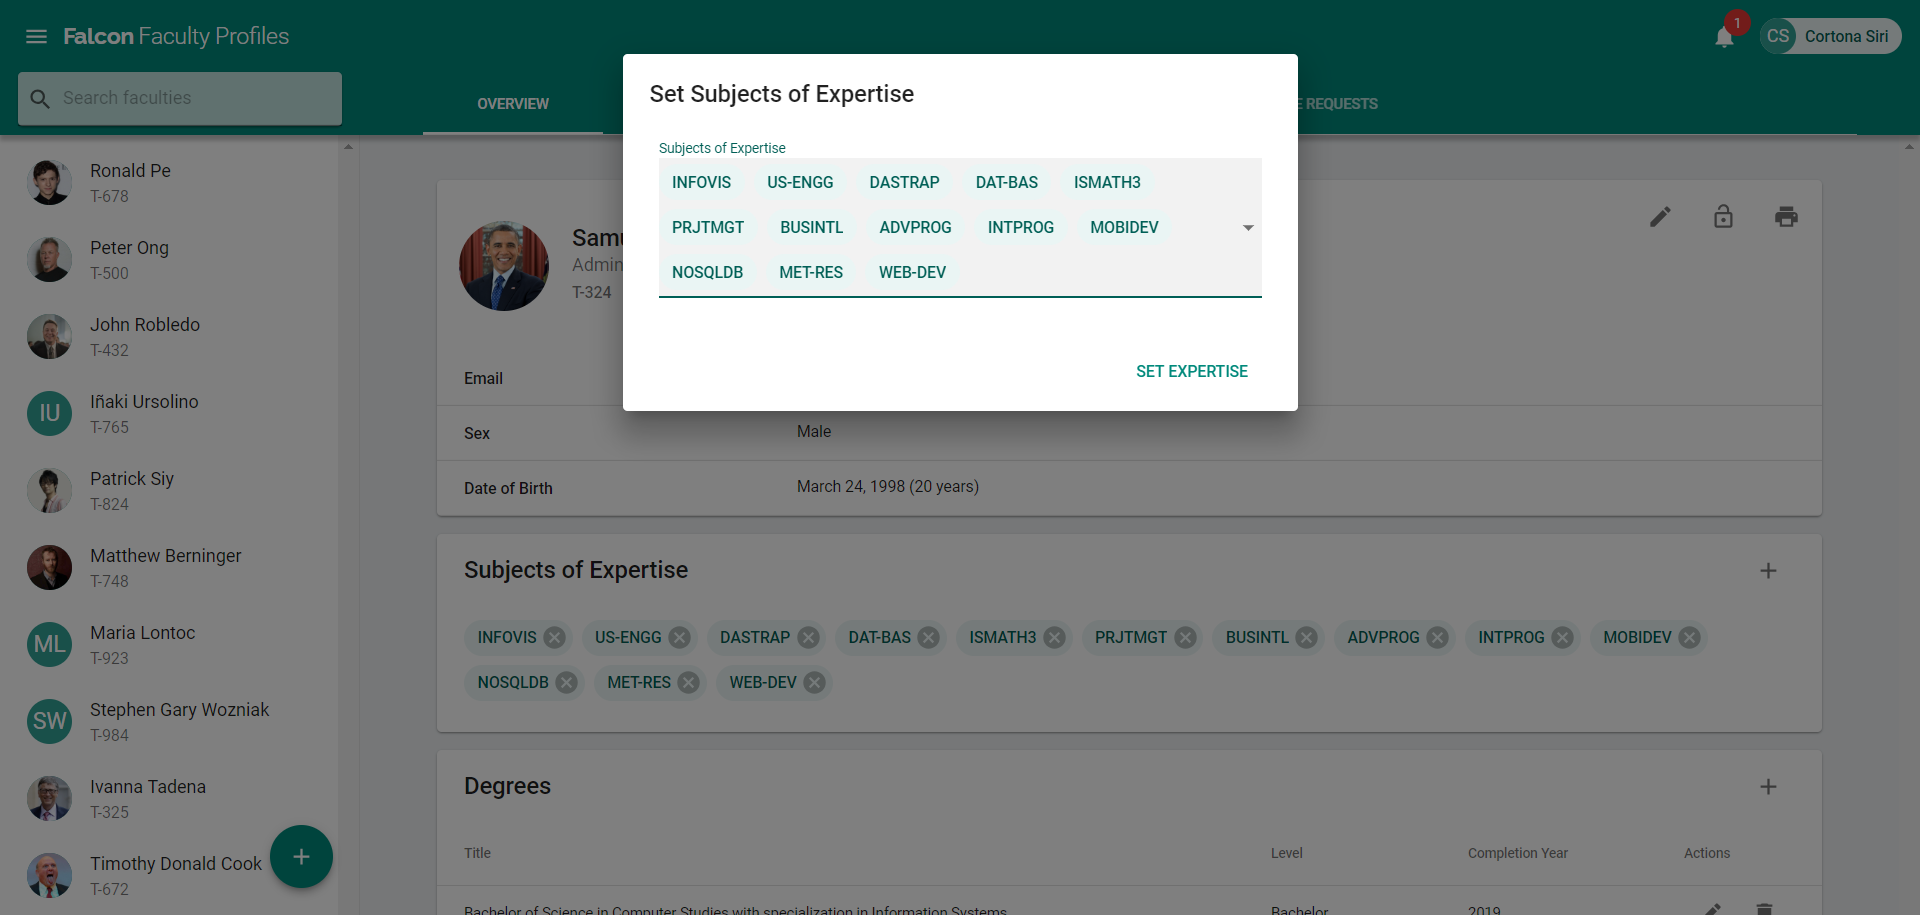
\includegraphics[width=\linewidth]{figures/form_specifications/set_expertise.png}
   \caption{Set Expertise}
   }
    
    \pagebreak
    

    
    \subsubsection{Add/Update Presentations}
    \field{Form Name}{Add/Update Presentations}
    
    \field{Description}{For users to add a new presentation to the faculty profile or update the details of an existing presentation.}
    
    \field{Prepared by}{Clerk}
    
    \field{Volume and Frequency:}{Added when the faculty accomplishes a new presentation, or when faculty has requested to add or update their presentations.}
    
    \field{Layout}{}
    
\makefigure{!h}{
   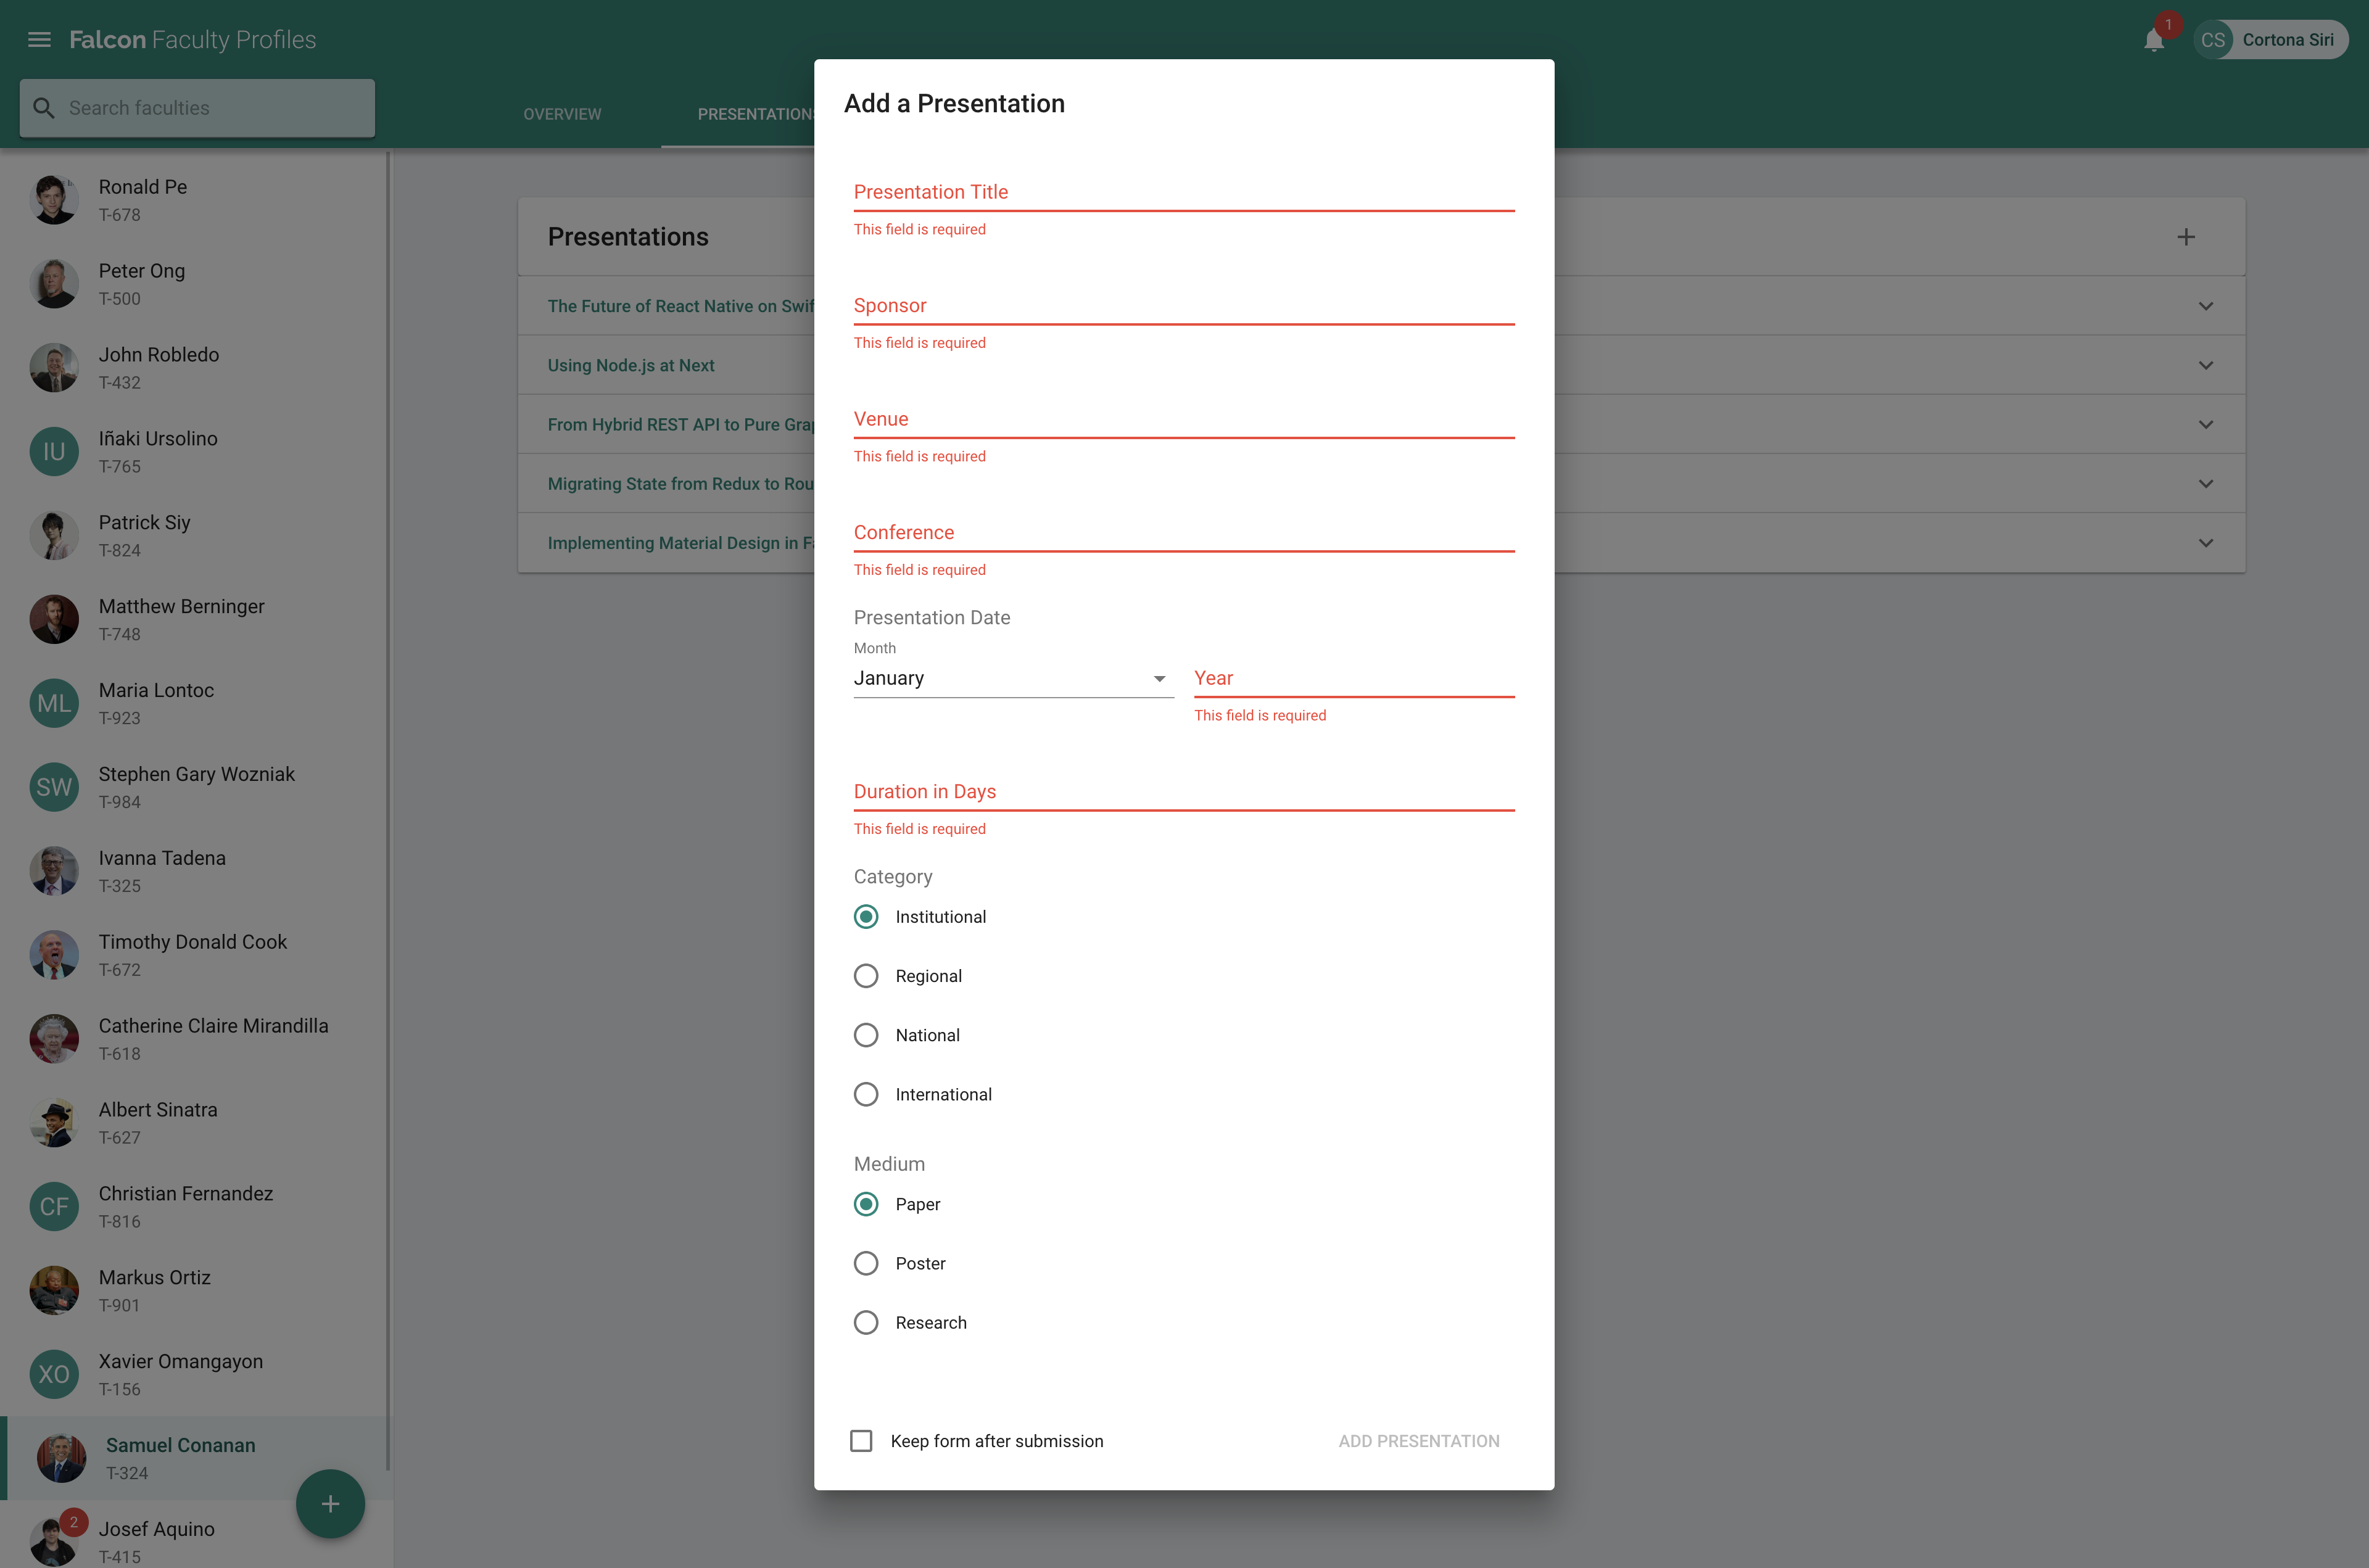
\includegraphics[width=\linewidth]{figures/form_specifications/add_presentation.png}
   \caption{Add/Update Presentation Screen}
}

    \pagebreak
    
    \subsubsection{Add/Update Instructional Materials}
    \field{Form Name}{Add/Update Instructional Materials}
    
    \field{Description}{For users to add a new instructional material or update the details of an existing instructional material.}
    
    \field{Prepared by}{Clerk}
    
    \field{Volume and Frequency}{Added when the faculty accomplishes a new presentation, or when faculty has requested to add or update their presentations.}
    
    \field{Layout}{}
    
\makefigure{!h}{
   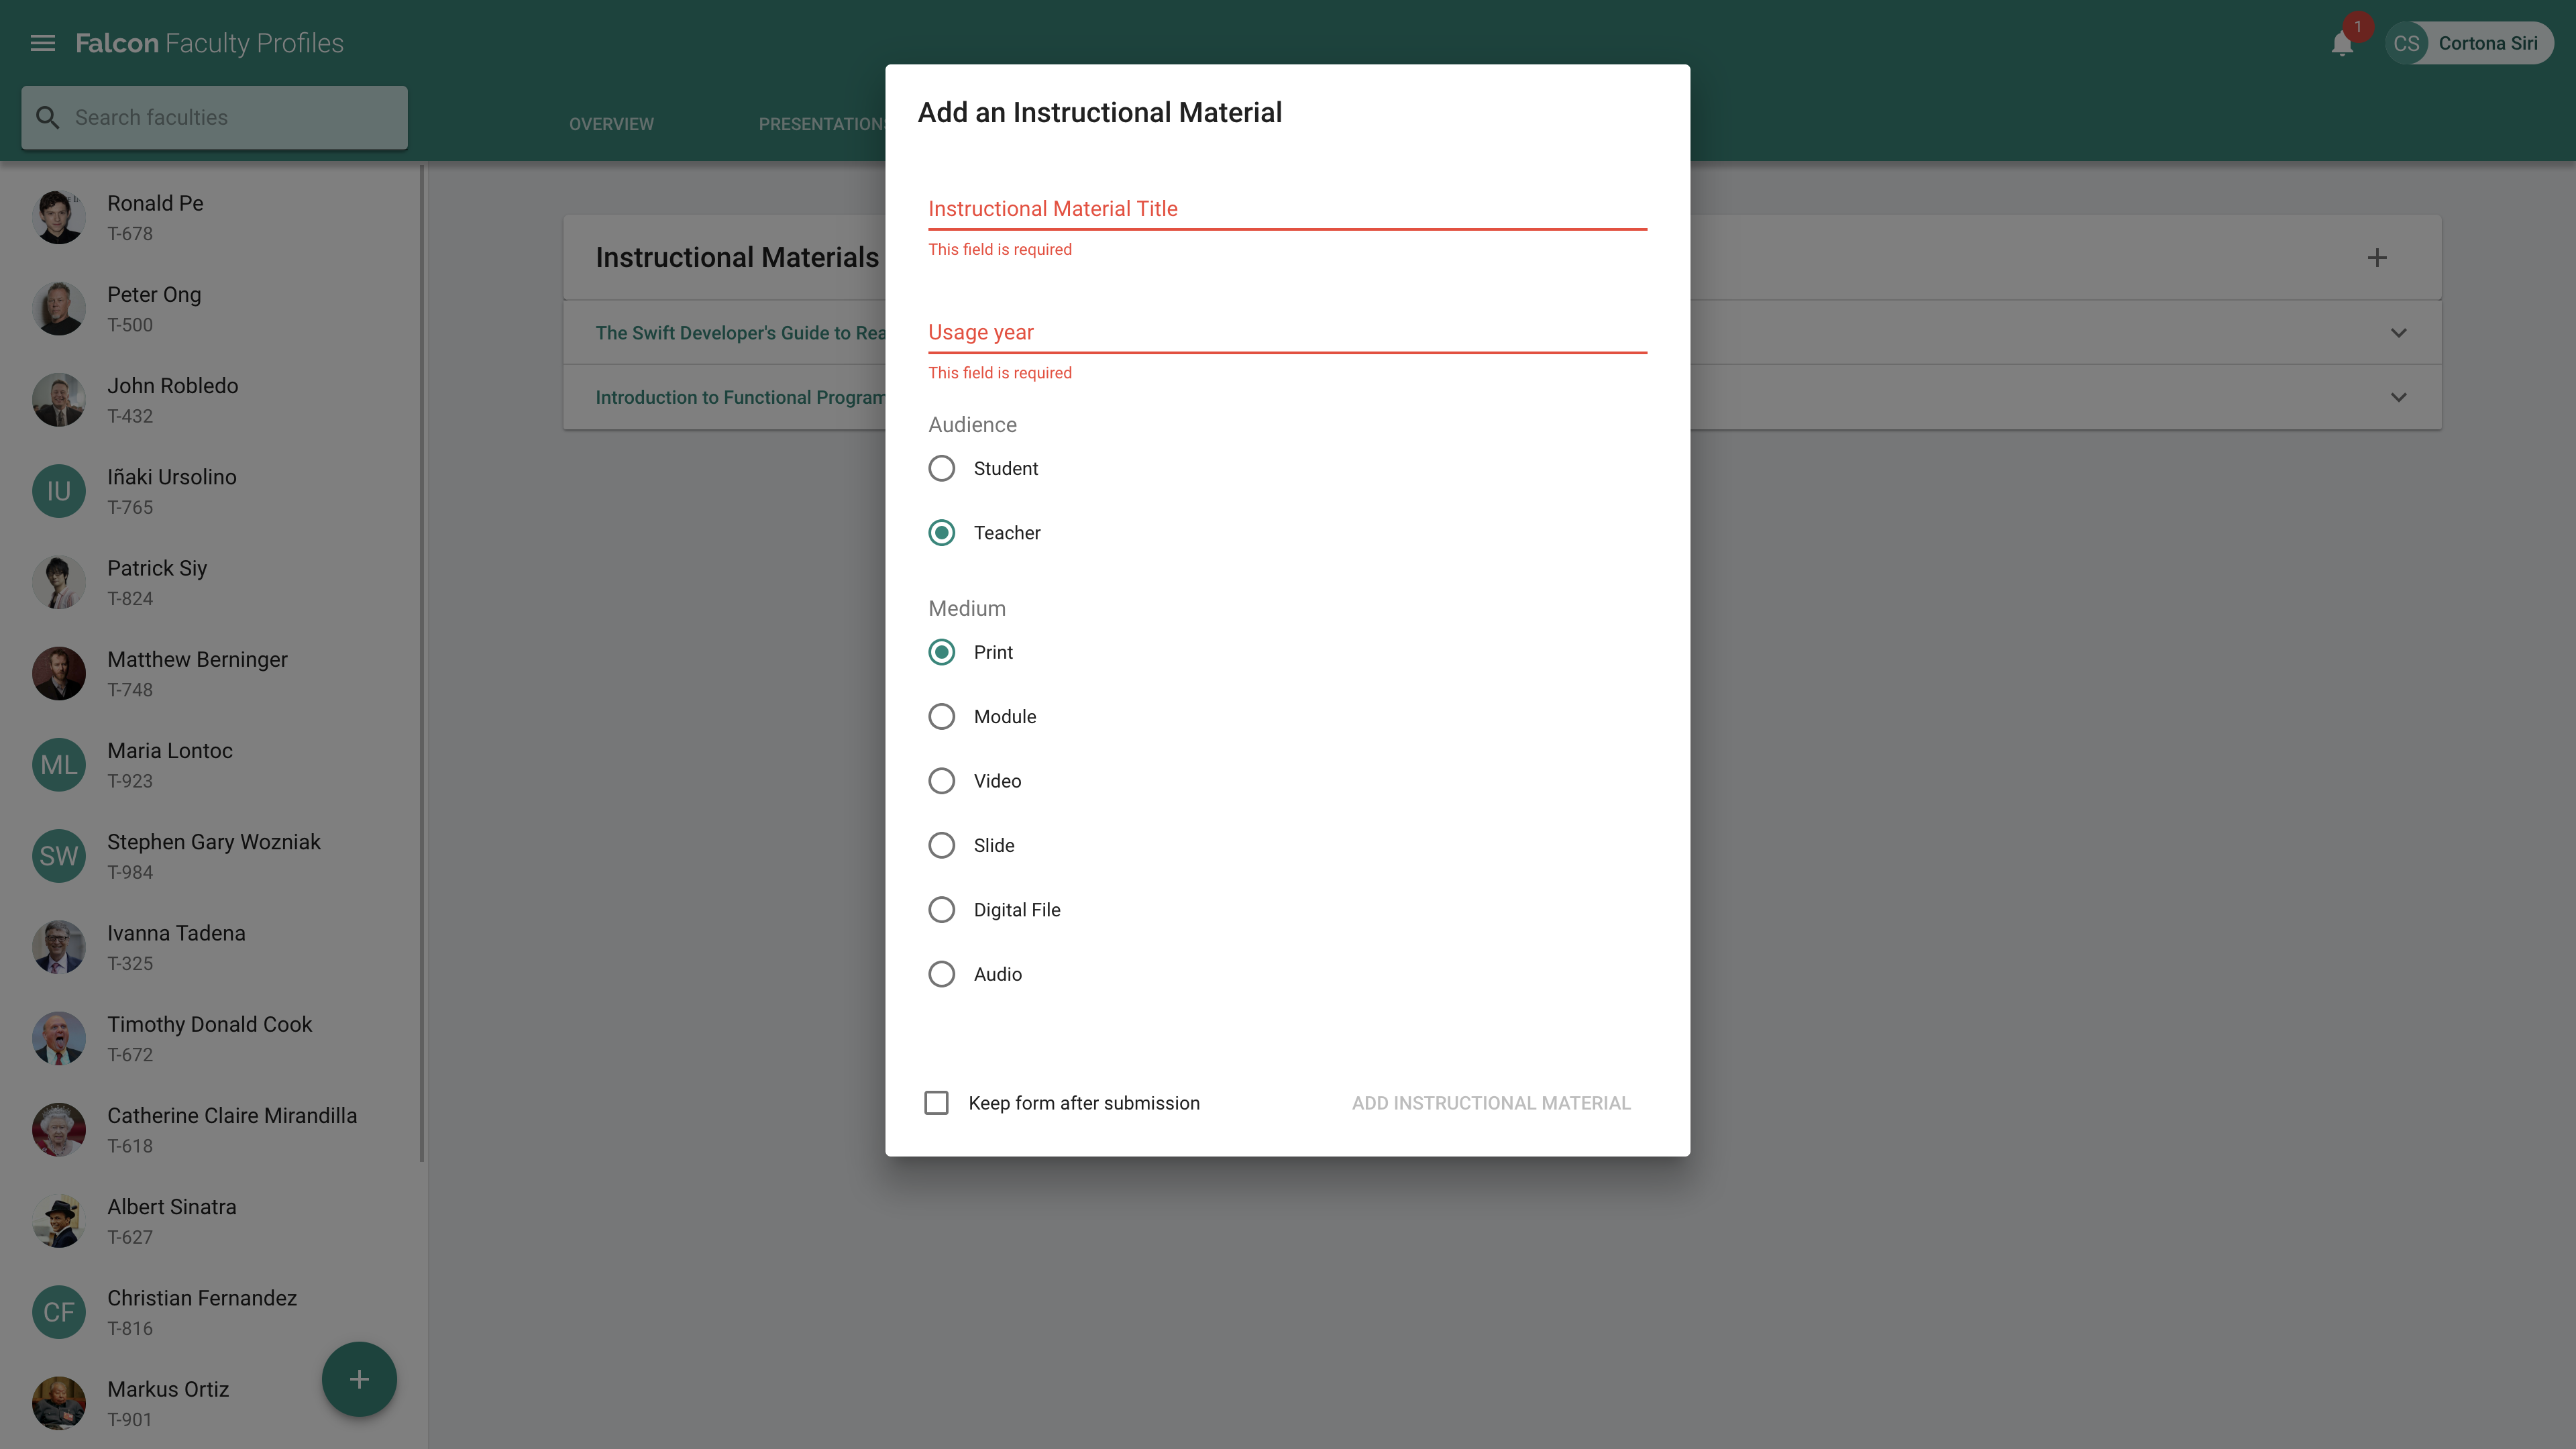
\includegraphics[width=\linewidth]{figures/form_specifications/add_instructional.png}
   \caption{Add/Update Instructional Material Screen}
   }
    \pagebreak
    
    \subsubsection{Add/Update Extension Works}
    \field{Form Name}{Add/Update Extension Work}
    
    \field{Description}{For the clerk to add a new extension work or update the details of an existing extension work.}
    
    \field{Prepared by}{Clerk}
    
    \field{Volume and Frequency}{Added when the faculty accomplishes a new extension work, or when faculty has requested to add or update their extension work.}
    
    \field{Layout}{} 
    
\makefigure{!h}{
   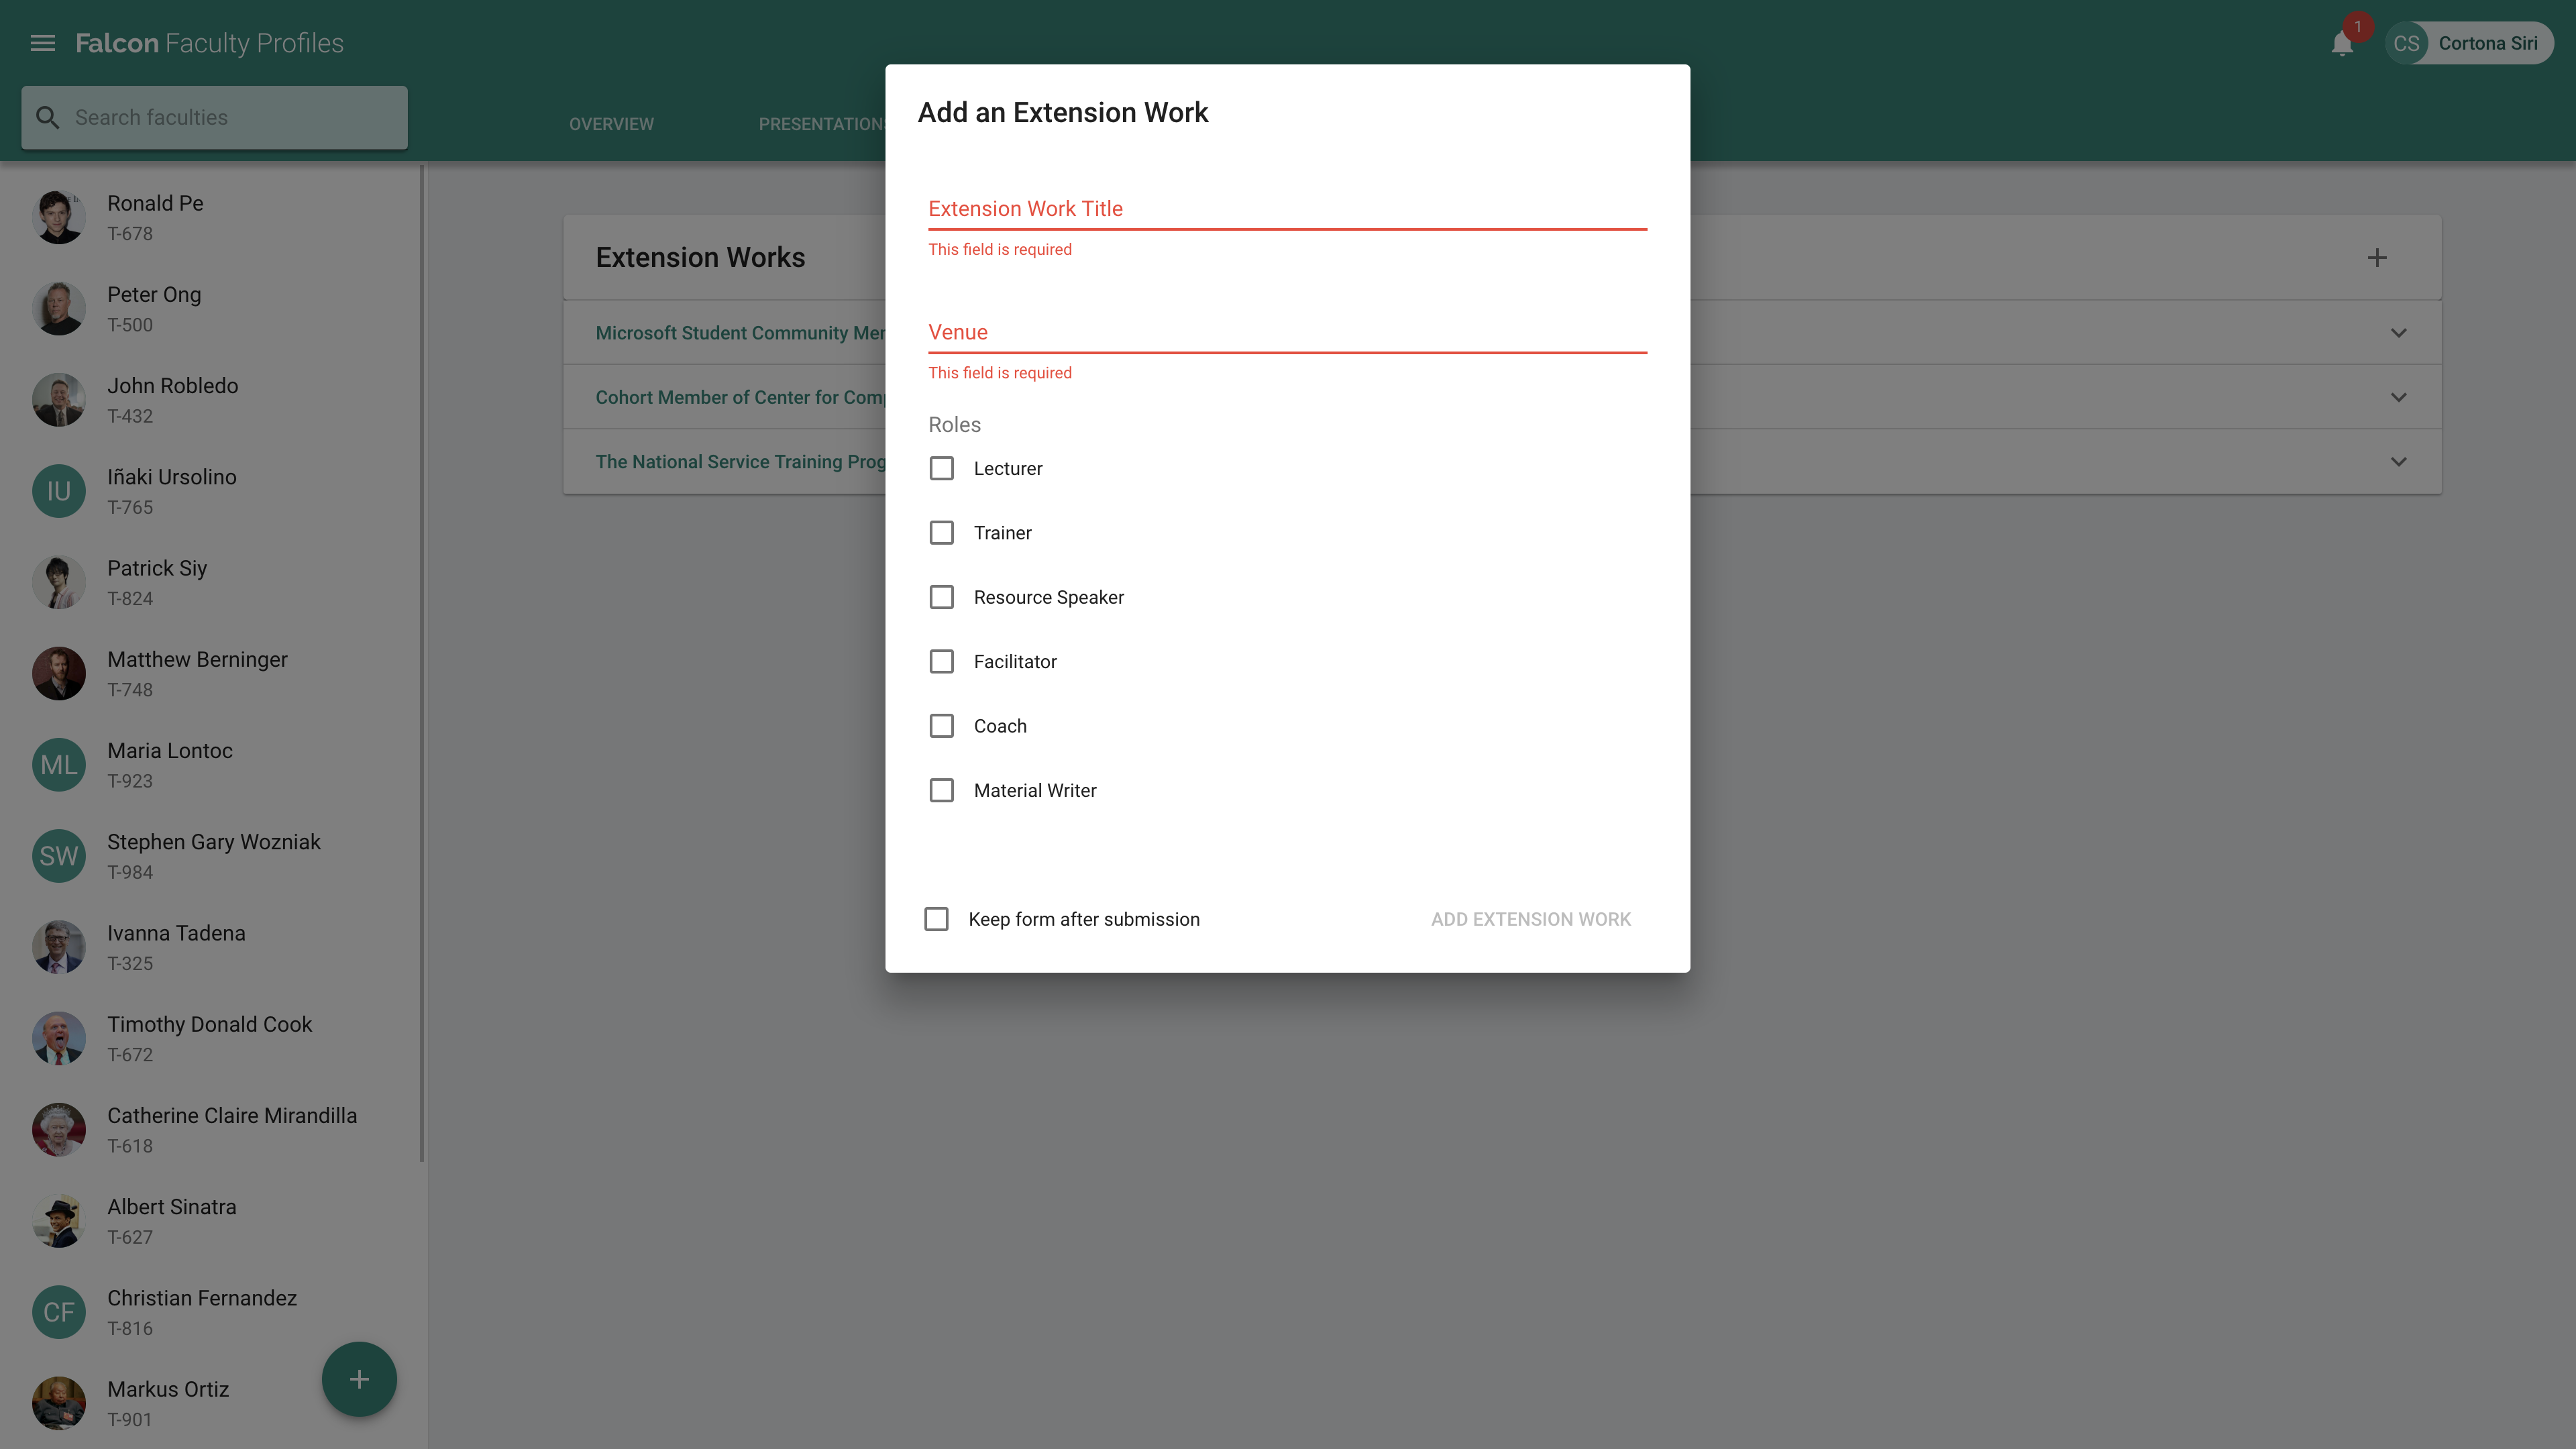
\includegraphics[width=\linewidth]{figures/form_specifications/add_extension.png}
   \caption{Add/Update Extension Work Screen}
   }
   
   \pagebreak
   
    \subsubsection{Rejection Reason}
    \field{Form Name}{Rejection Reason}
    
    \field{Description}{When rejecting a change request, the clerk inputs the reason behind the rejection through this form.}
    
    \field{Prepared by}{Clerk}
    
    \field{Volume and Frequency}{When a change request is rejected}
    
    \field{Layout}{} 
    
\makefigure{!h}{
   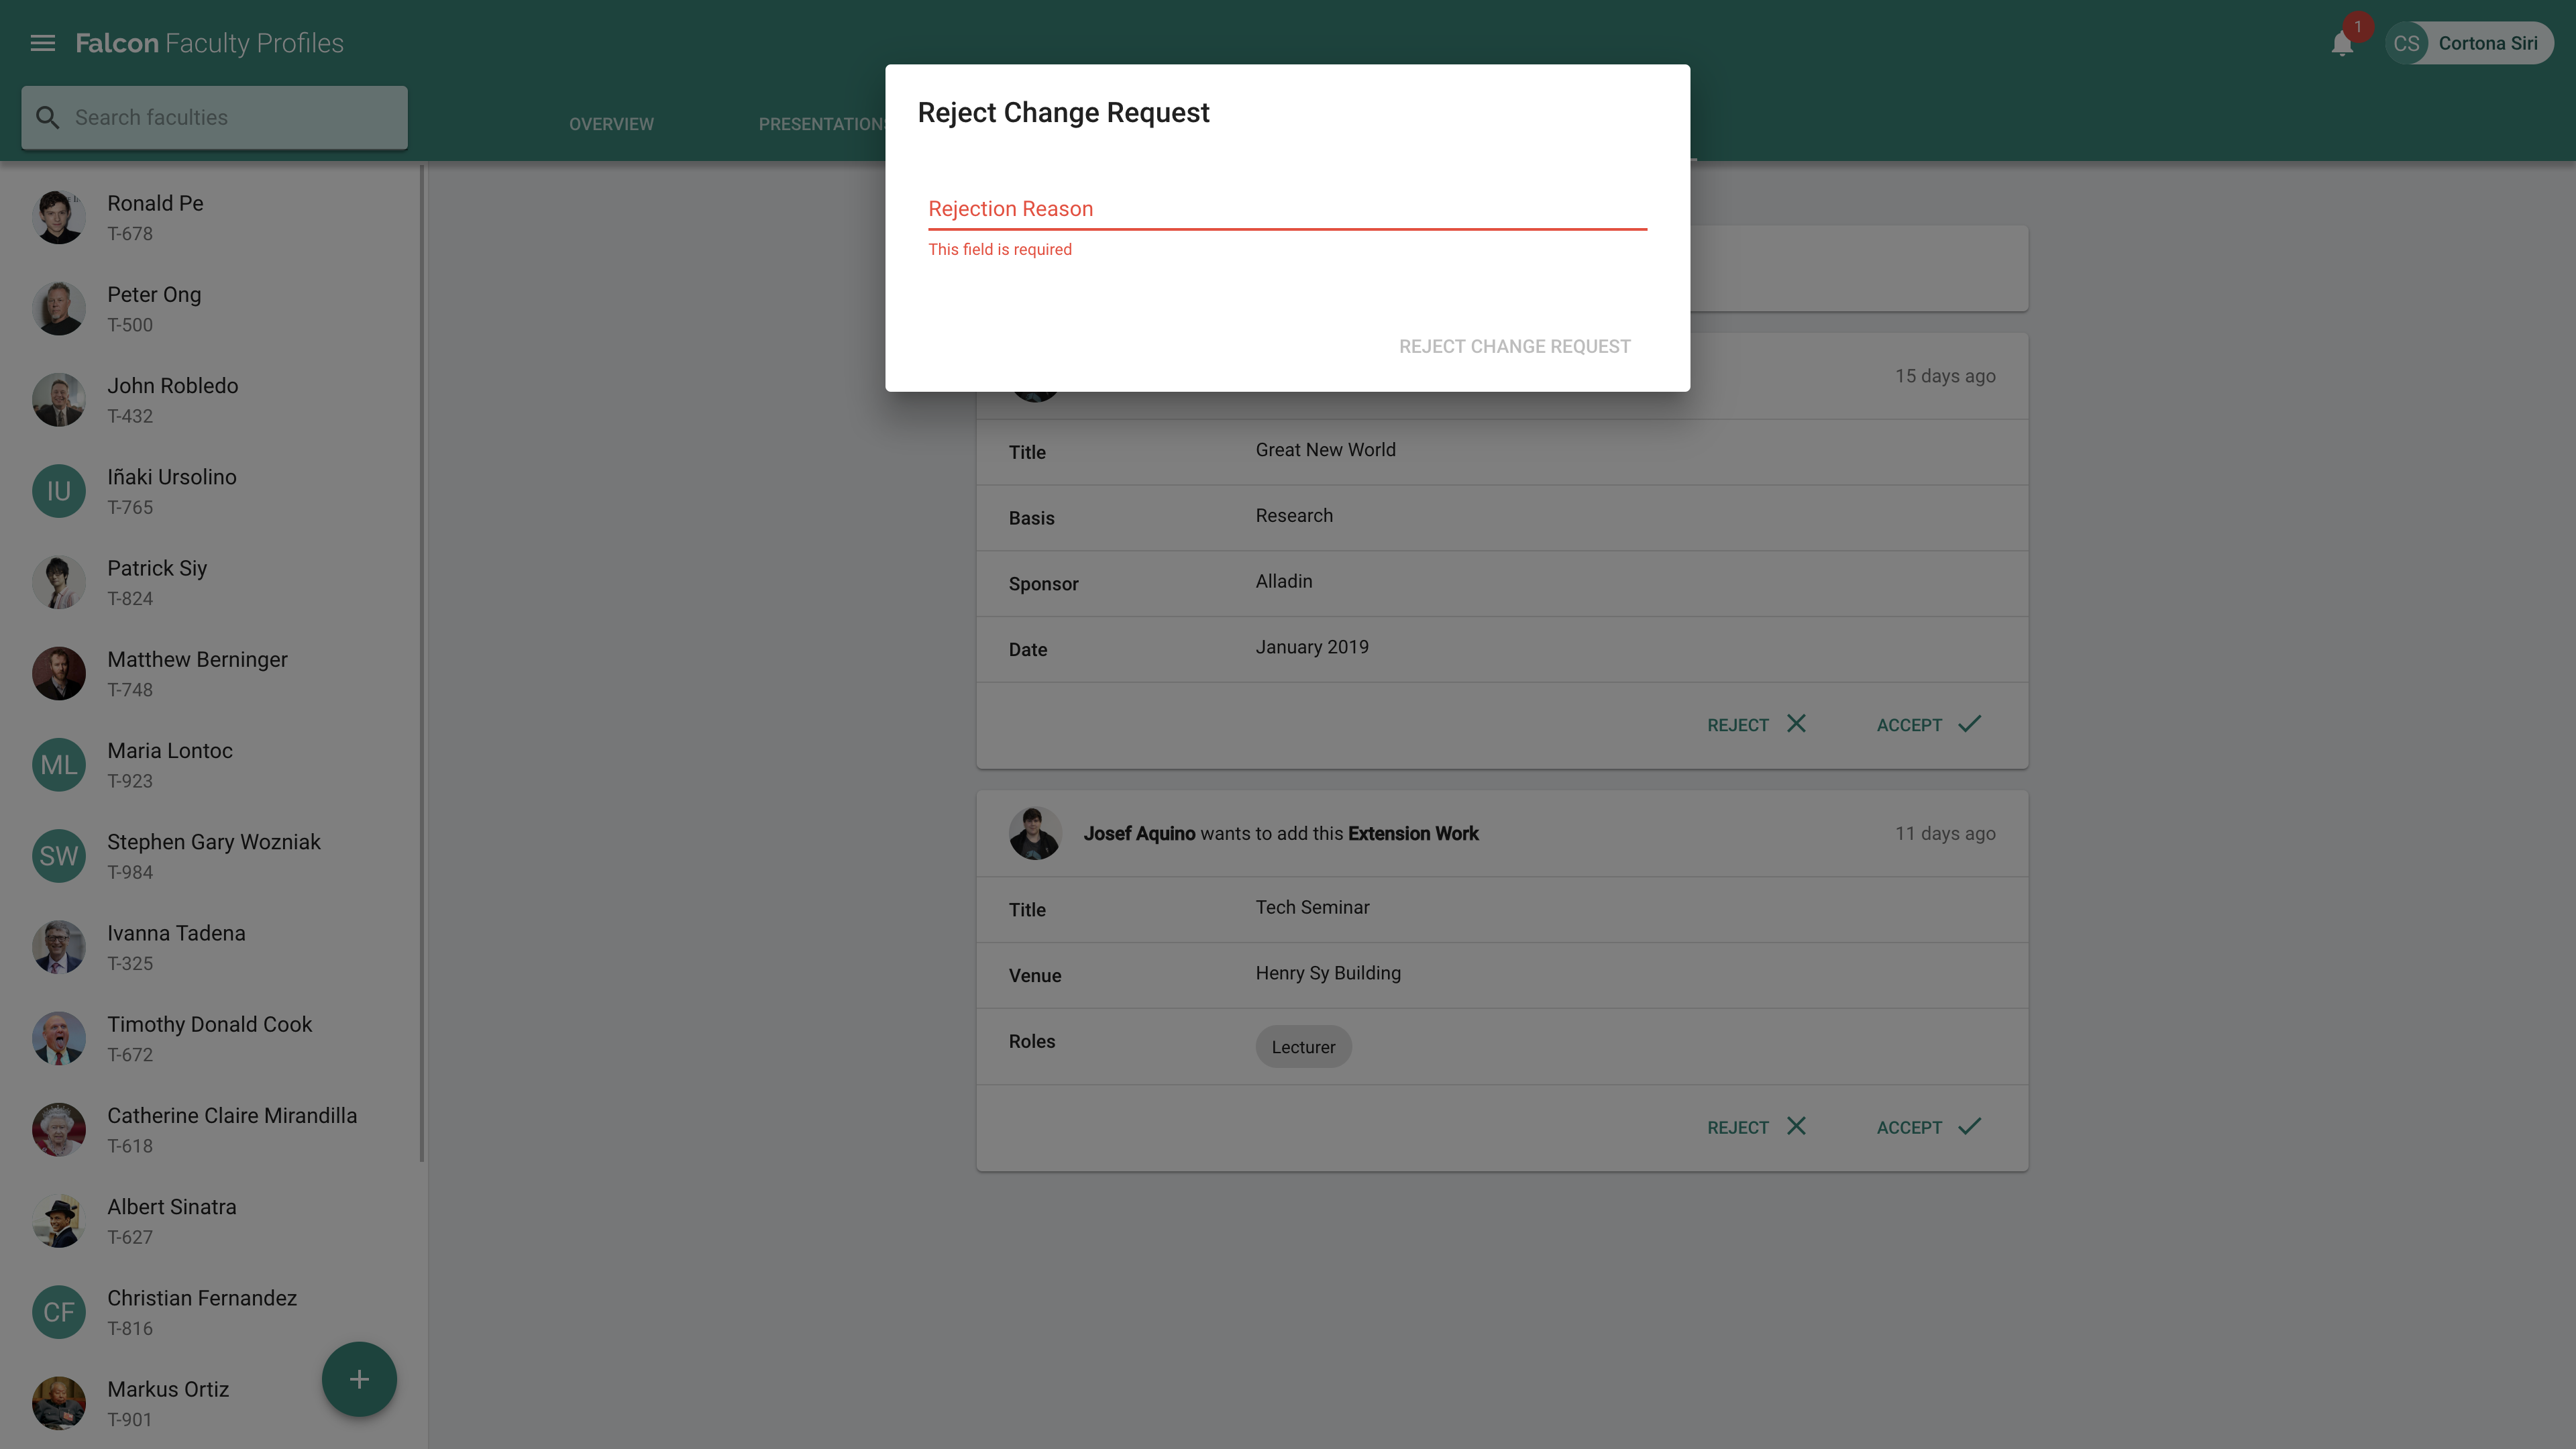
\includegraphics[width=\linewidth]{figures/form_specifications/rejection_reason.png}
   \caption{Rejection Reason Screen}
   }
   
   \pagebreak
   
   
   \subsection{My Profile}
    
    \subsubsection{Request Add/Update Degree}
    
    \field{Form Name}{Request Add Degree}
    
    \field{Description}{For the faculty member to request to add or update a degree to their faculty profile.}
    
    \field{Prepared by}{Faculty Member}
    
    \field{Volume and Frequency}{Added when the faculty member needs to add or update a degree.}
    
    \field{Layout}{}
    
\makefigure{!h}{
   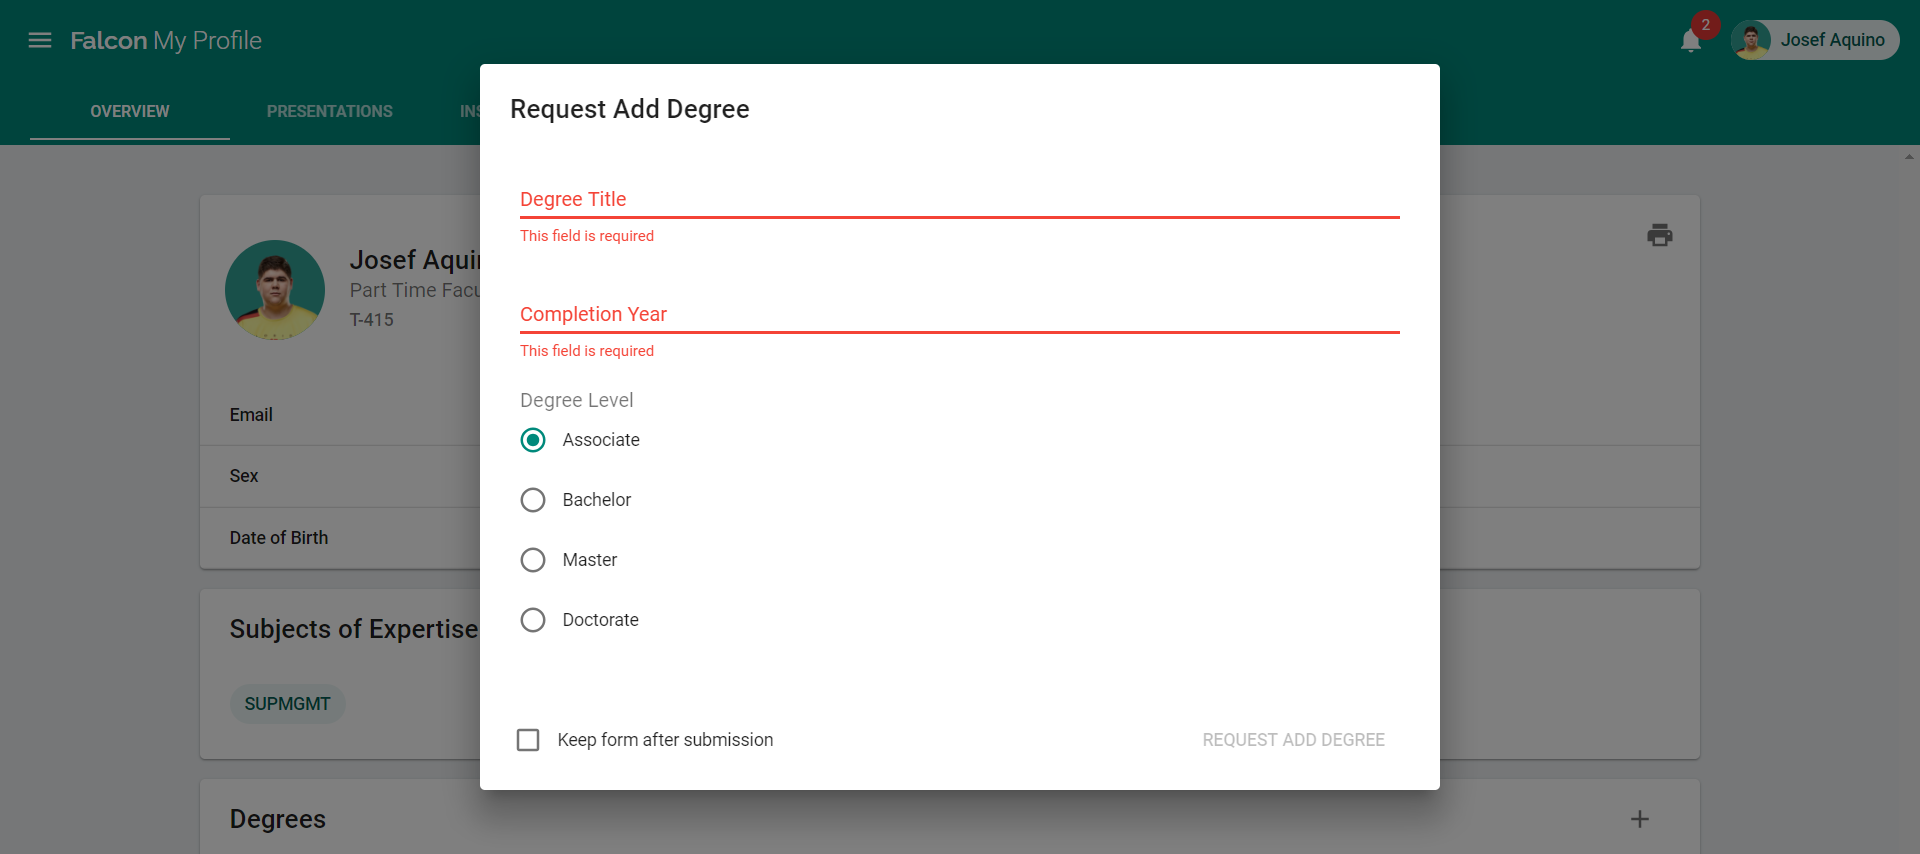
\includegraphics[width=\linewidth]{figures/form_specifications/myprofile_forms/my_profile_add_degree.png}
   \caption{Request Add Degree Screen}
}
\pagebreak

    \subsubsection{Request Add/Update Recognition}
    
    \field{Form Name}{Request Add Recognition}
    
    \field{Description}{For the faculty member to request to add or update a recognition to their faculty profile.}
    
    \field{Prepared by}{Faculty Member}
    
    \field{Volume and Frequency}{Added when the faculty member needs to add or update a recognition.}
    
    \field{Layout}{}
    
\makefigure{!h}{
   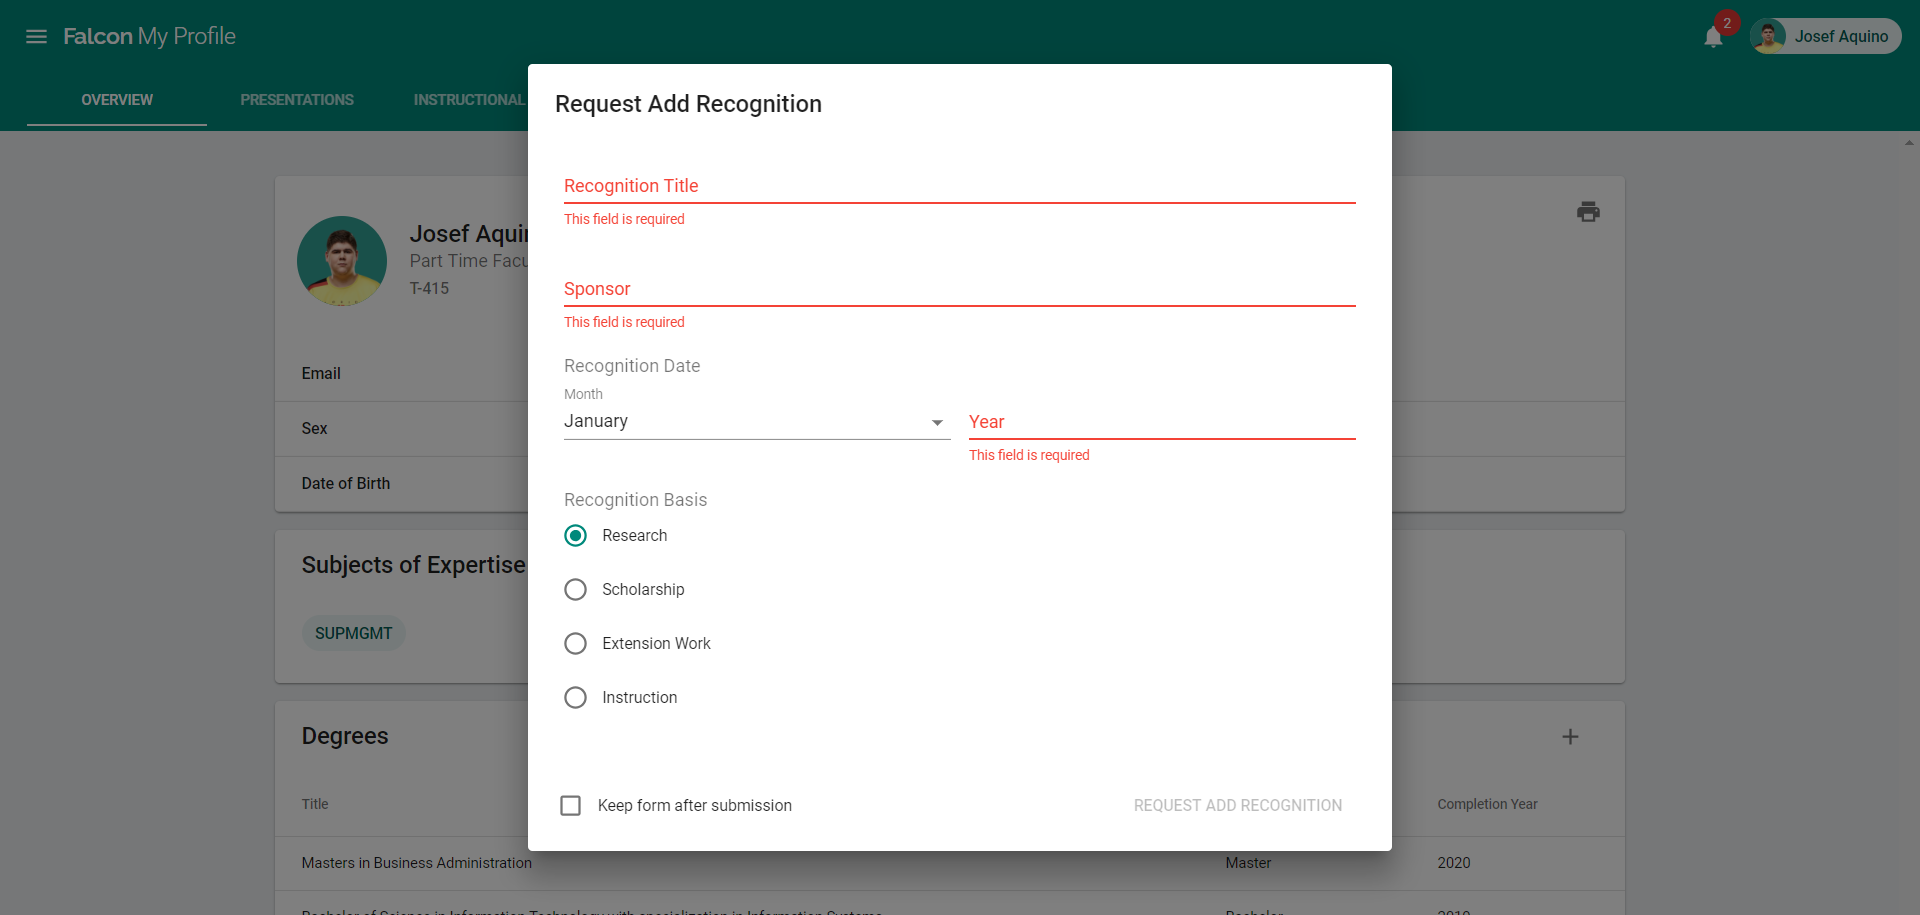
\includegraphics[width=\linewidth]{figures/form_specifications/myprofile_forms/my_profile_add_recognition.png}
   \caption{Request Add Recognition Screen}
}
\pagebreak

    \subsubsection{Request Add/Update Presentation}
    
    \field{Form Name}{Request Add Presentation}
    
    \field{Description}{For the faculty member to request to add or update a presentation to their faculty profile.}
    
    \field{Prepared by}{Faculty Member}
    
    \field{Volume and Frequency}{Added when the faculty member needs to add or update a presentation.}
    
    \field{Layout}{}
    
\makefigure{!h}{
   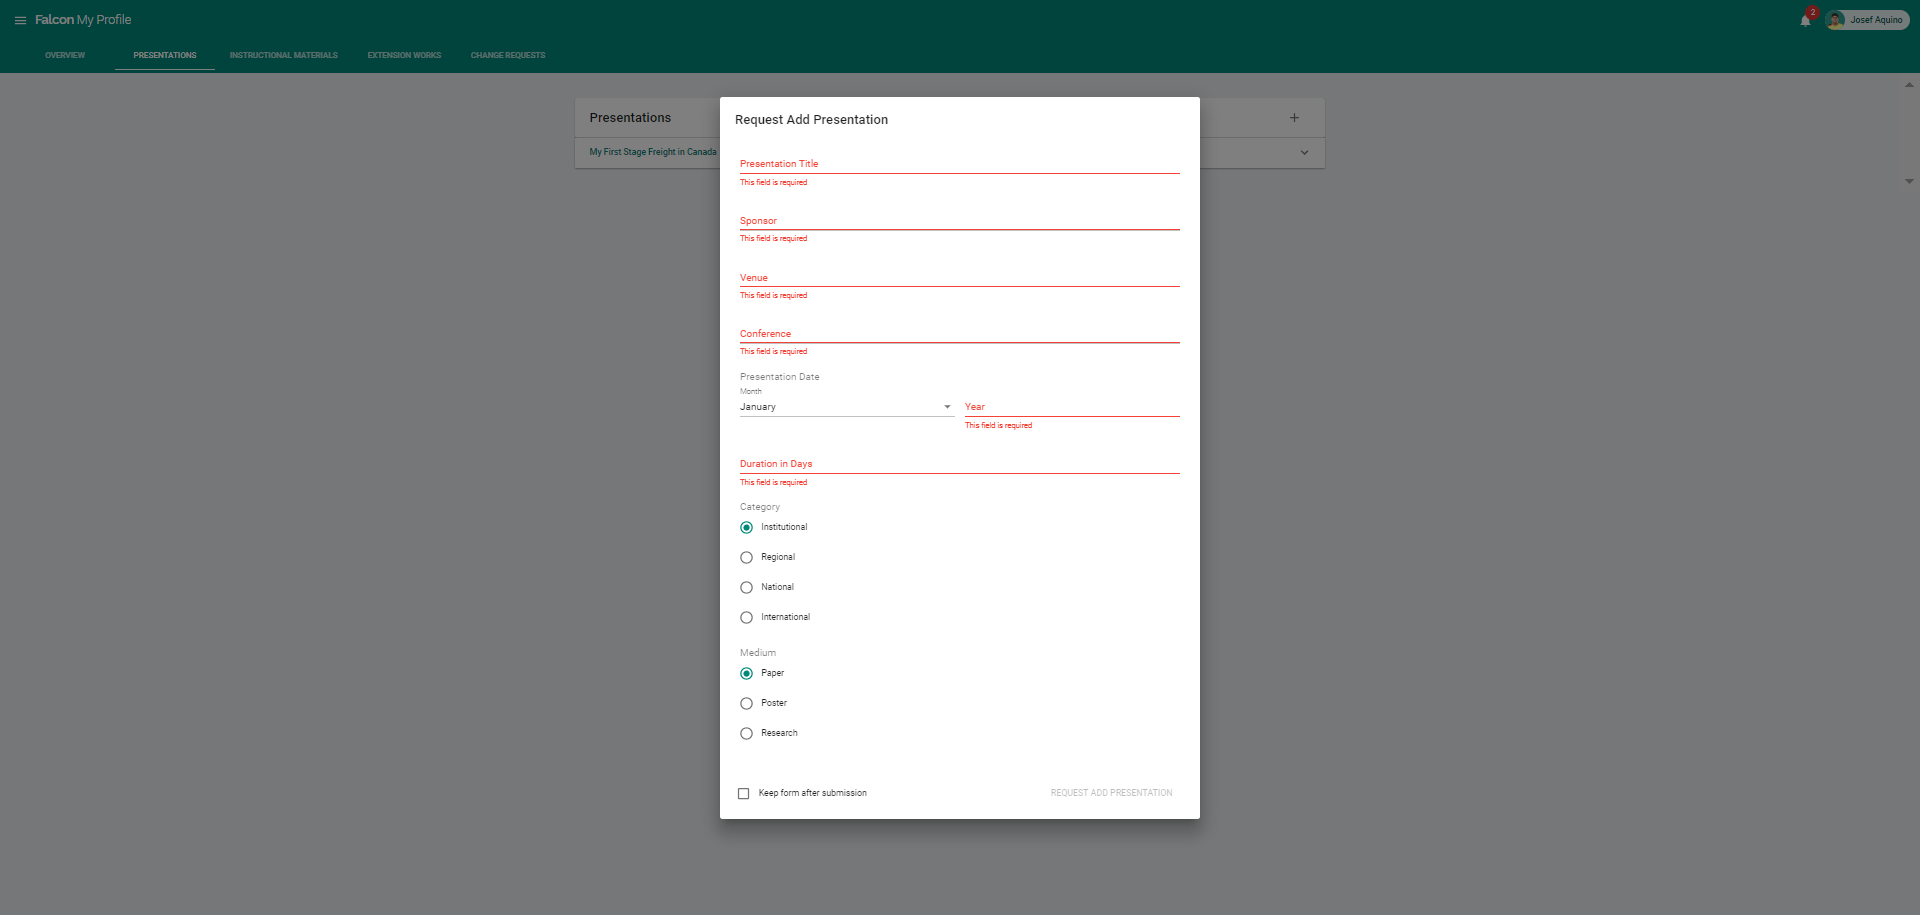
\includegraphics[width=\linewidth]{figures/form_specifications/myprofile_forms/my_profile_add_presentation.png}
   \caption{Request Add Presentation Screen}
}
\pagebreak

    \subsubsection{Request Add/Update Instructional Material}
    
    \field{Form Name}{Request Add Instructional Material}
    
    \field{Description}{For the faculty member to request to add an instructional material or update the details of an existing instructional material to their faculty profile.}
    
    \field{Prepared by}{Faculty Member}
    
    \field{Volume and Frequency}{}
    
    \field{Layout}{}
    
\makefigure{!h}{
   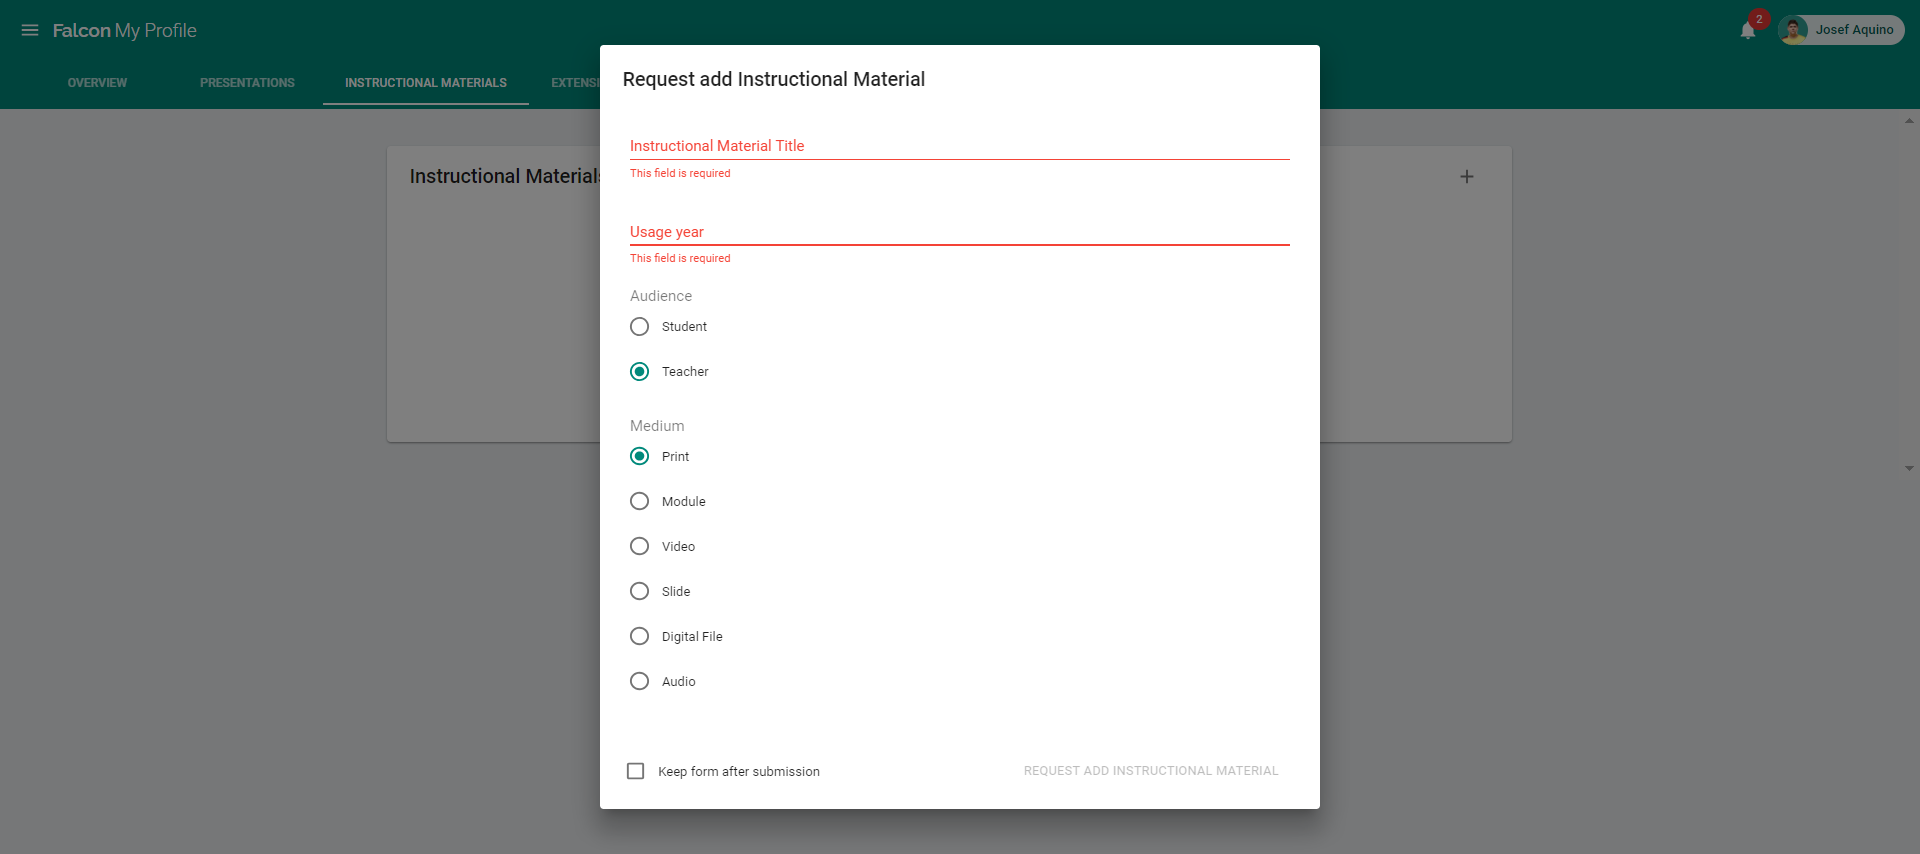
\includegraphics[width=\linewidth]{figures/form_specifications/myprofile_forms/my_profile_add_instructional.png}
   \caption{Request Add Instructional Material Screen}
}
\pagebreak

    \subsubsection{Request Add/Update Extension Work}
    
    \field{Form Name}{Request Add Extension Work}
    
    \field{Description}{For the faculty member to request to add an extension work or update the details of an existing extension work to their faculty profile.}
    
    \field{Prepared by}{Faculty Member}
    
    \field{Volume and Frequency}{Added when the faculty member needs to add or update an extension work.}
    
    \field{Layout}{}
    
\makefigure{!h}{
   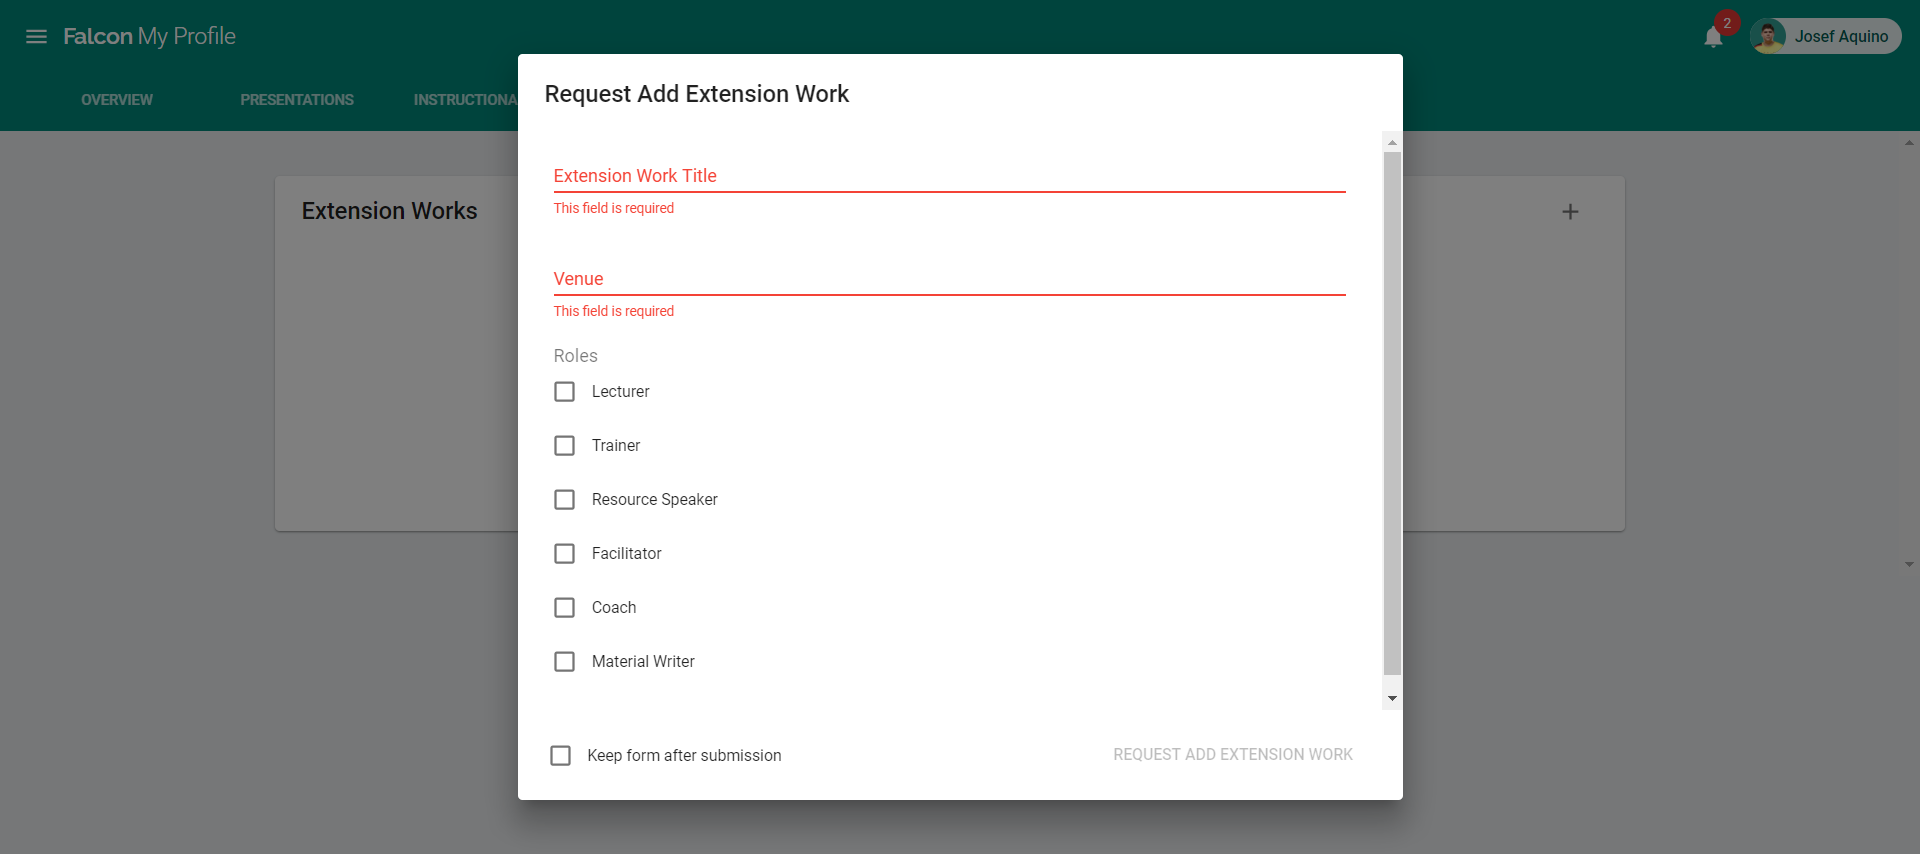
\includegraphics[width=\linewidth]{figures/form_specifications/myprofile_forms/my_profile_add_extension.png}
   \caption{Request Add Extension Work Screen}
}
\pagebreak

    \subsubsection{Change My Password}
    
    \field{Form Name}{Change My Password}
    
    \field{Description}{For faculty members to input and confirm their new password after it has been reset.}
    
    \field{Prepared by}{Faculty Member}
    
    \field{Volume and Frequency}{Filled whenever a faculty member has had their password reset.}
    
    \field{Layout}{}
    
\makefigure{!h}{
   \includegraphics[width=\linewidth]{figures/form_specifications/myprofile_forms/change_my_password.png}
   \caption{Change My Password Screen}
}
\pagebreak
    
\section{Report Specifications}

\subsubsection{Faculty Profile}
    
    \field{Report Name}{Faculty Profile Report}
    
    \field{Description}{For the clerk to generate a report of a faculty profile}
    
    \field{Prepared by}{Clerk}
    
    \field{Volume and Frequency}{Created when requested or when faculty members are have to submit it.}
    
    \field{Layout}{}
    
\makefigure{!h}{
   \includegraphics[width=\linewidth]{figures/report_specifications/faculty_profile_report1.png}
   \caption{Faculty Profile Report 1}
}

\makefigure{!h}{
   \includegraphics[width=\linewidth]{figures/report_specifications/faculty_profile_report2.png}
   \caption{Faculty Profile Report 2}
}

\makefigure{!h}{
   \includegraphics[width=\linewidth]{figures/report_specifications/faculty_profile_report3.png}
   \caption{Faculty Profile Report 3}
}

\makefigure{!h}{
   \includegraphics[width=\linewidth]{figures/report_specifications/faculty_profile_report4.png}
   \caption{Faculty Profile Report 4}
}

\makefigure{!h}{
   \includegraphics[width=\linewidth]{figures/report_specifications/faculty_profile_report5.png}
   \caption{Faculty Profile Report 5}
}
\pagebreak